%%%%%%%%%%%%%%%%%%%% book.tex %%%%%%%%%%%%%%%%%%%%%%%%%%%%%
%
% sample root file for the chapters of your "monograph"
%
% Use this file as a template for your own input.
%
%%%%%%%%%%%%%%%% Springer-Verlag %%%%%%%%%%%%%%%%%%%%%%%%%%


% RECOMMENDED %%%%%%%%%%%%%%%%%%%%%%%%%%%%%%%%%%%%%%%%%%%%%%%%%%%
\documentclass[graybox,envcountchap,sectrefs]{svmono}

% choose options for [] as required from the list
% in the Reference Guide

%\usepackage{mathptmx}
%\usepackage{helvet}
%\usepackage{courier}
%
\usepackage{type1cm}   
\usepackage{chapterbib}
\usepackage{cite}
\usepackage{subfigure}
\usepackage{makeidx}         % allows index generation
\usepackage{graphicx}        % standard LaTeX graphics tool
\usepackage{siunitx}         % when including figure files
\usepackage{multicol}        % used for the two-column index
\usepackage{multirow}
\usepackage[bottom]{footmisc}% places footnotes at page bottom
\usepackage{enumerate}
\usepackage{newtxtext}       % 
\usepackage{newtxmath}       % selects Times Roman as basic font
\usepackage{booktabs}
\usepackage{multirow}
\usepackage{tikz}
\usepackage[ruled,linesnumbered]{algorithm2e}

% see the list of further useful packages
% in the Reference Guide

\makeindex             % used for the subject index
                       % please use the style svind.ist with
                       % your makeindex program

%%%%%%%%%%%%%%%%%%%%%%%%%%%%%%%%%%%%%%%%%%%%%%%%%%%%%%%%%%%%%%%%%%%%%
% User defined commands
\newtheorem{exmp}{\bf Example\,}[section]

\graphicspath{{./}{images/}}

\newcommand*\circled[1]{\tikz[baseline=(char.base)]{
    \node[shape=circle,draw,inner sep=0.6pt,color=white, fill=black] (char) {#1};}}

\newcommand*\rectangle[1]{\tikz[baseline=(char.base)]{
    \node (rect) [draw,inner sep=1.8pt,color=white, fill=black,minimum width=2pt,minimum height = 2pt] (char) {#1};}}
\newcommand{\RNum}[1]{\uppercase\expandafter{\romannumeral #1\relax}}

\begin{document}

\author{Xiaowei Li, Guihai Yan, Cheng Liu}
\title{Built-In Fault-Tolerant Computing Paradigm for Resilient Large-Scale Chip Design}
%\subtitle{-- A Self-Test, Self-Diagnosis, and Self-Repair Approach}
\maketitle

\frontmatter%%%%%%%%%%%%%%%%%%%%%%%%%%%%%%%%%%%%%%%%%%%%%%%%%%%%%%


%%%%%%%%%%%%%%%%%%%%%%% dedic.tex %%%%%%%%%%%%%%%%%%%%%%%%%%%%%%%%%
%
% sample dedication
%
% Use this file as a template for your own input.
%
%%%%%%%%%%%%%%%%%%%%%%%% Springer %%%%%%%%%%%%%%%%%%%%%%%%%%

\begin{dedication}
To all the stundets and colleagues in Integrated Circuit Design Group in State Key Lab of Computer Architecture.
\end{dedication}





%%%%%%%%%%%%%%%%%%%%%%foreword.tex%%%%%%%%%%%%%%%%%%%%%%%%%%%%%%%%%
% sample foreword
%
% Use this file as a template for your own input.
%
%%%%%%%%%%%%%%%%%%%%%%%% Springer %%%%%%%%%%%%%%%%%%%%%%%%%%

\foreword

%% Please have the foreword written here
Use the template \textit{foreword.tex} together with the document class SVMono (monograph-type books) or SVMult (edited books) to style your foreword\index{foreword}. 

The foreword covers introductory remarks preceding the text of a book that are written by a \textit{person other than the author or editor} of the book. If applicable, the foreword precedes the preface which is written by the author or editor of the book.


\vspace{\baselineskip}
\begin{flushright}\noindent
Place, month year\hfill {\it Firstname  Surname}\\
\end{flushright}



%%%%%%%%%%%%%%%%%%%%%%preface.tex%%%%%%%%%%%%%%%%%%%%%%%%%%%%%%%%%%%%%%%%%
% sample preface
%
% Use this file as a template for your own input.
%
%%%%%%%%%%%%%%%%%%%%%%%% Springer %%%%%%%%%%%%%%%%%%%%%%%%%%

\preface

%% Please write your preface here
If your computer crashes, you can revive it by a reboot, an empirical solution that usually turns out to be effective. The rationale behind this solution is that transient faults, either in hardware or software, can be fixed by refreshing the machine state. Such a “silver bullet”, however, could be futile in the future because the faults, especially those existing in the hardware such as Integrated Circuit (IC) chips, cannot be eliminated by refreshing. What we need is a more sophisticated mechanism to steer the system back to the right track. The “magic cure” is the on-chip fault-tolerant mechanism, which relies on a suite of built-in design-for-reliability logic, including fault detection, fault diagnosis, and fault recovery, working in a unified manner. 

In the past decade, we have successfully applied the proposed fault-tolerant computing mechanism onto various chip designs including generic circuits, general purposed processors, network-on-chips, and deep learning processors and gradually formulate an systematic built-in on-chip fault-tolerant computing paradigm, which can be utilized to guide IC designs against faults caused by manufacture defects, radiation particles, or progressively aging. In addition to the basic fault detection, fault diagnosis, and fault recovery, the proposed on-chip fault-tolerant computing paradigm also provides attractive benefits, such as facilitating graceful performance degradation, mitigating the impact of verification blind spots, and improving the chip yield.

In this book, we mainly illustrate the built-in on-chip fault-tolerant computing paradigm with demonstrations on genetic circuits, general purposed processors, network-on-chips, and deep learning processors. The entire book consists of 6 chapters. Chapter 1 presents the background of fault-tolerant chip designs and overview of the fault-tolerant computing paradigm. Chapter 2, Chapter3, Chapter 4, and Chapter 5 demonstrate the use of the proposed fault-tolerant computing paradigm on specific areas of chips including generic circuits, general purposed processors, network-on-chips, and deep learning processors respectively. Chapter 6 concludes this book with a brief summary of this book and discussion of future directions.

The techniques involved in this book are collected from thesis of Guihai Yan, Lei Zhang, Songjun Pan, Cheng Liu, Wen Li supervised by Prof. Xiaowei Li. All the relevant materials are already published in the leading conferences and journals in VLSI design and EDA. Prof. Xiaowei Li organized this book in general, Prof. Cheng Liu finished Chapter 1, Chapter 4, Chapter 5, and Chapter 6, Prof. Guihai Yan mainly finished Chapter 2 and Chapter 3. Prof. XX and Prof. XXX reviewed this book and Prof. Tim Cheng wrote Foreword for this book. All the efforts are greatly appreciated.

The techniques presented in this book are partly selected from research founded by XXX, XXX, XXX, and XXX. 

\vspace{\baselineskip}
\begin{flushright}\noindent
\leftline{Institute of Computing Technology, Haidian, Beijing} \\
May 2022\hfill {\it Xiaowei Li}\\
\end{flushright}



%%%%%%%%%%%%%%%%%%%%%%acknow.tex%%%%%%%%%%%%%%%%%%%%%%%%%%%%%%%%%%%%%%%%%
% sample acknowledgement chapter
%
% Use this file as a template for your own input.
%
%%%%%%%%%%%%%%%%%%%%%%%% Springer %%%%%%%%%%%%%%%%%%%%%%%%%%

\extrachap{Acknowledgements}

Use the template \emph{acknow.tex} together with the document class SVMono (monograph-type books) or SVMult (edited books) if you prefer to set your acknowledgement section as a separate chapter instead of including it as last part of your preface.



\tableofcontents

%%%%%%%%%%%%%%%%%%%%%%acronym.tex%%%%%%%%%%%%%%%%%%%%%%%%%%%%%%%%%%%%%%%%%
% sample list of acronyms
%
% Use this file as a template for your own input.
%
%%%%%%%%%%%%%%%%%%%%%%%% Springer %%%%%%%%%%%%%%%%%%%%%%%%%%

\extrachap{Acronyms}

Use the template \emph{acronym.tex} together with the document class SVMono (monograph-type books) or SVMult (edited books) to style your list(s) of abbreviations or symbols.

Lists of abbreviations\index{acronyms, list of}, symbols\index{symbols, list of} and the like are easily formatted with the help of the Springer-enhanced \verb|description| environment.

\begin{description}[CABR]
\item[ABC]{Spelled-out abbreviation and definition}
\item[BABI]{Spelled-out abbreviation and definition}
\item[CABR]{Spelled-out abbreviation and definition}
\end{description}


\mainmatter%%%%%%%%%%%%%%%%%%%%%%%%%%%%%%%%%%%%%%%%%%%%%%%%%%%%%%%
%%%%%%%%%%%%%%%%%%%%%%part.tex%%%%%%%%%%%%%%%%%%%%%%%%%%%%%%%%%%
% 
% sample part title
%
% Use this file as a template for your own input.
%
%%%%%%%%%%%%%%%%%%%%%%%% Springer %%%%%%%%%%%%%%%%%%%%%%%%%%

\begin{partbacktext}
\part{Part Title}
\noindent Use the template \emph{part.tex} together with the document class SVMono (monograph-type books) or SVMult (edited books) to style your part title page and, if desired, a short introductory text (maximum one page) on its verso page.

\end{partbacktext}
%%%%%%%%%%%%%%%%%%%%% chapter.tex %%%%%%%%%%%%%%%%%%%%%%%%%%%%%%%%%
%
% sample chapter
%
% Use this file as a template for your own input.
%
%%%%%%%%%%%%%%%%%%%%%%%% Springer-Verlag %%%%%%%%%%%%%%%%%%%%%%%%%%
%\motto{Use the template \emph{chapter.tex} to style the various elements of your chapter content.}
\chapter{Introduction} \label{sec:intro}

\abstract{xxx}

\section{Typical On-Chip Faults} \label{sec:sec1.1}
To be added.

\subsection{Process Variation}
To be added.

\subsection{Manufacturing Defects}
To be added.

\subsection{Chip Aging}
The on-chip fault tolerance paradigm can help maintain the lifetime reliability of microprocessors suffering in-field degradation ascribed to both silicon devices and metal wires. The degraded silicon (including the devices and wires) is metaphorically called “Sick Silicon” \cite{yan2015corerank}. According to International Technology Roadmap For Semiconductors (ITRS) projection, silicon aging tops the impending (above 22 nm) reliability challenges. The industry and academic communities have performed significant work to understand the failure mechanisms of semiconductor devices, such as electromigration (EM), bias temperature instability (BTI) including negative and positive BTI (also known as NBTI and PBTI, respectively), time dependent dielectric breakdown (TDDB), hot carrier injection, and temperature cycling, etc. Both NBTI and TDDB draw the most attention concerning several transistor aging mechanisms. Both of them can gradually degrade performance over time. The researchers have evidence that circuit path delay can increase by 10\% during the five-year lifetime \cite{wang2007impact}. Even worse, with technology scaling to the nano-scale, the transistors tend to become more vulnerable and more prone to aging impacts \cite{wang2007impact}. 

The integrity of the wires is also degraded. The shrinking size leads to increased current density. Increased current density causes aggravated EM effects, which also contribute to the in-filed performance and reliability degradation. The effects of EM produce increased resistance of the wires and thereby result in increased RC delay. The increasing delay will eventually outgrow the timing margin and, even worse, the wires will eventually breakdown, causing break faults, bridge faults, or stuck-at faults in the chips. 

Since the whole chip is exposed to these aging mechanisms, some parts of the chip suffer faster aging than the others. The main reason can be attributed the following two aspects.

First, the “weak” chips, which are more sensitive to aging, mainly results from process variations \cite{borkar2003parameter}. As the feature size relentlessly shrinks generation-by-generation, the impacts of process variations become increasingly evident. Because of the wafer-to-wafer, die-to-die, and within-die variations, the proportion of the circuits with serious mismatches to the golden reference in the design print should be marked as weak silicon and removed from the production batch as yield loss. For example, the typical threshold voltage $V_{th}$ of transistors may exhibit obvious deviations from the standard settings because of width/length fluctuations caused by an unstable lithographic process. Those transistors with the elevated $V_{th}$ have smaller tolerances to withstand the aging induced $V_{th}$ increasing and are therefore prone to be more sensitive to it than those with larger tolerances.

Second, the aging rate of silicon devices (including the metal wires) depends not only on the intrinsic constitution of the devices themselves, but also on the stressing duty cycles [12]. From a microscopic perspective, the data patterns, which determine the BTI aging degree, are intrinsically non-uniform across the all bits. Consequently, some transistors are always positively or negatively-biased and therefore degrade much faster than those that are evenly-biased. The heavily-biased BTI aging has a slight chance to enjoy the recovery effect, which exacerbates the aging degree. From a microarchitectural perspective, for another example, the usage of some cores in a multicore processor could be always higher than the others because an oracle round-robin scheduling algorithm is not an option in modern operating system (OS) design. The jobs assigned to different cores can show very distinct stressing degrees. The computationally intensive jobs are usually more power-hungry and therefore generate more heat which can speed up the aging, while those computationally non-intensive jobs are the opposite.

\subsection{Soft Errors}
To be added.

\subsection{Intermittent Faults}
Intermittent hardware faults occur frequently and irregularly for a period of time, commonly due to manufacturing residuals, oxide degradation, process variations, and in-progress wear-out. Although intermittent faults and soft errors may manifest similar effects, there are several differences between them. First, from the spatial aspect, an intermittent fault occurs repeatedly at the same location, while a soft error rarely occurs in the same place. Second, from the temporal aspect, an intermittent fault will occur at burst, while a soft error is usually a single event upset or a single event transient. Third, if an affected structure has been replaced, intermittent faults will be eliminated; soft errors, however, can not be reduced by repair. There are also some differences between intermittent faults and hard faults. A hard fault exists during the lifetime of a chip and continually generates errors if the failing device is exercised, while an intermittent fault may be periodically activated and deactivated due to process and environmental variations. Intermittent faults also may turn to hard faults finally \cite{smolens2007detecting}.

An intermittent fault has three key parameters: burst length (BL), active time (AT), and inactive time (IAT) \cite{gracia2008analysis}. Burst length is the lifetime of an intermittent fault; active time is the positive pulse width of one activation, while inactive time is the time between two consecutive activations. The relationship among the three parameters can be expressed as $BL=N \times {AT} + (N - 1) \times IAT$ where represents the number of activations in an intermittent fault. These three parameters determine the characteristics of an intermittent fault, and their values can be dissimilar for different intermittent fault configurations. Fig. \ref{fig:intermittent-faults} shows the temporal feature of intermittent faults within a period of time. Intermittent faults have adverse impact on program execution only during their active time. The time interval between two consecutive bursts is called safe time which means no intermittent fault occurs during that time, and the safe time could be varied because the occurrence of an intermittent fault is uncertain.

\begin{figure}[t]
\centering
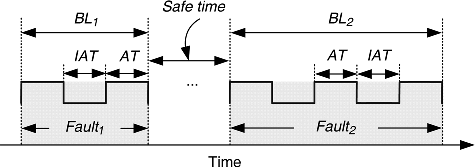
\includegraphics[scale=0.75]{IVF-fig1}
\caption{Key parameters of intermittent faults}
\label{fig:intermittent-faults} 
\end{figure}

In order to characterize the vulnerability of microprocessor structures to intermittent faults, it is important to establish appropriate logic fault models for them. The established logic fault models should represent physical intermittent abnormal phenomena that occur in real microprocessors. Based on the root causes and behaviors, intermittent faults can be classified into the following fault models \cite{gracia2008analysis} \cite{gil2003study}.

\begin{itemize}
    \item \textit{Intermittent stuck-at faults (including intermittent stuck-at-1 and stuck-at-0 faults):} Intermittent stuck-at faults are caused by residues in storage cells or solder joints during manufacturing. Unlike a soft error to upset a bit, an intermittent stuck-at fault transforms the correct value on the faulty signal line intermittently to be stuck at a constant value, either a logic value “1” or a logic value “0”. Structures most vulnerable to intermittent stuck-at faults are storage structures, such as memory and register file. In this work, we assume an intermittent stuck-at fault only causes one-bit of corruption.

    \item \textit{Intermittent open and short faults:} Intermittent open and short faults are usually caused by electro-migration, stress migration, or intermittent contacts. Intermittent open faults are breaks or imperfections in circuit interconnections such as wires, contacts, transistors and so forth. Intermittent short faults are shorts in wires or shorts in transistors. If an element being intermittently shorted to power or ground , it is equivalent to an intermittent stuck-at fault. If two signal wires are shorted together, an intermittent bridging fault occurs \cite{wang2006vlsi}. Fig. \ref{fig:open-short-faults} illustrates several examples of intermittent open and short faults. The circuit consists of a two-input NOR gate and a NOT gate. is an intermittent open fault in transistor , while is an intermittent open fault in wire C. is an intermittent short fault to in wire D and is an intermittent bridging fault. Intermittent open and short faults may turn to hard faults if existing for a long time. Elements most vulnerable to these faults are signal buses and I/O connections.

    \item \textit{Intermittent timing faults:} Intermittent timing faults are mainly caused by inductive noises, aging, crosstalk, or process, voltage, temperature (PVT) variations. Intermittent timing faults will result in timing violations and affect data propagation when they occur. They usually lead to write wrong data to storage cells (i.e., flip-flops miss to latch the newly computed value due to path-delay) and finally become reliability problems. Intermittent timing faults can be broadly classified into intermittent path-delay faults and intermittent transition faults. In this work, we  mainly focus on intermittent path-delay faults. Besides, an intermittent timing fault may affect multiple bits of the data captured by storage structures or just a single bit in a structure. For example, a crosstalk induced delay fault may either affect multiple data lines or only one data line. We only consider the former situation that an intermittent timing fault affects multiple data lines.
\end{itemize}

\begin{figure}[t]
\centering
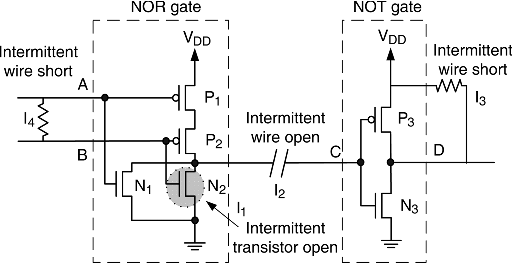
\includegraphics[scale=0.75]{IVF-fig2}
\caption{Examples of different intermittent open and short faults}
\label{fig:open-short-faults} 
\end{figure}

\begin{figure}[t]
\centering
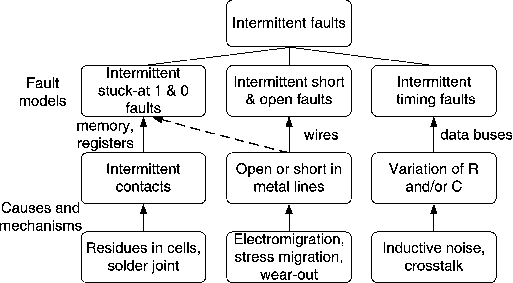
\includegraphics[scale=0.75]{IVF-fig3}
\caption{Physical causes, mechanisms, and fault models for intermittent faults}
\label{fig:fault-cause} 
\end{figure}


Fig. \ref{fig:fault-cause} summarizes the main physical causes, mechanisms, and fault models for intermittent faults. Each kind of fault model has different causes, behaviors, and its own representative analysis method. Although the causes of these fault models may be different, they may have some physical causes in common. For example, the situation that an open or short in metal lines also can lead to intermittent stuck-at faults, such as the fault in Fig. \ref{fig:open-short-faults}.

As we need to estimate the vulnerability of different microprocessor structures to intermittent faults, it is necessary to know the probability distribution of intermittent faults after establishing fault models. Srinivasan et al. \cite{srinivasan2005exploiting} show intermittent open and short faults obey log-normal distributions during the lifetime of microprocessors, which means the failure rate is low at the beginning of a microprocessor’s lifetime and it will grow as the microprocessor ages. Intermittent stuck-at faults and intermittent timing faults mainly obey uniform distribution and are highly dependent on the applications. To facilitate the analysis, we make the following assumption in this work: intermittent faults occur with high frequency and obey uniform distribution during program execution. The high intermittent fault rate is consistent with the public consideration of future industry technologies \cite{borkar2003parameter}. Although we only concentrate on the uniform distribution for intermittent faults, our evaluation methodology is also suitable to analyze other statistical distributions of intermittent faults.

\subsection{Emerging Technologies Induced Defects}
To be added.

\section{Conventional Wisdom for Fault-Tolerant Chip Design}
\subsection{Design for Test}
To be added.

\subsection{Design for Reliability}
To be added.

\section{On-Chip Fault-Tolerant Computing Paradigm}
Reliability is one of the mainstay merits of virtually any computing system. Beyond conventional fault tolerance computing \cite{borkar2005designing}, built-in on-chip fault tolerance faces several unique challenges: (1) Resource limited. On-chip fault tolerance is engaged during the duty time so that any dedicated automatic testing equipment (ATE) are unavailable. Therefore, the only viable strategy is to build all required test supports on the chip, which makes the on-chip fault tolerance mechanism operate in a self-supporting manner. (2) Overhead-sensitive. Even though silicon has become increasingly cheap thanks to the Moore's law, it is still unwise to extravagantly use the silicon for non-performance goals. For ordinary users, it is probably highly risky for the chip makers tout for customers with the probability of a system crash rather than the more appreciable performance.

Over the past decade, we have exploited the on-chip fault tolerance to build a holistic solution ranging from on-chip fault detection to error recovery mechanisms \cite{yan2011revivenet, fu2011abacus,  yan2015corerank, yan2010svfd, zhang2009topology, han2013revivepath, liu2021hyca}. We applied them to generic circuits, processing cores, Network-On-Chip
(NoC), deep learning processors. The on-chip fault tolerance framework usually consists of three key components: self-test, self-diagnosis, self-repair, or '3S framework' for short. Some prototypes have been built to demonstrate how on-chip fault tolerance responds to the in-filed silicon degradation. More interestingly, we find that the 3S framework is not only a powerful backbone guiding various on-chip fault tolerance designs and implementations, but also has more far-reaching implications such as maintaining graceful performance degradation, mitigating the impact of verification blind spots, and improving the chip yield. We believe that these design principles will be critical for the chip makers to maintain a competitive edge in the future.

As a fault tolerance mechanism, on-chip fault tolerance has the ingredients of generic fault tolerance mechanisms: fault detection, fault diagnosis, and fault recovery. Fault detection is used to judge whether the system suffers from erroneous executions, then fault diagnosis digs deeper to determine where and how such errors happen, which is followed by a recovery routine to correct the error to the expected outcomes. For the on-chip fault tolerance, the generic framework evolves with several new attributes which provide the essences of the self-supportive 3S approach.

\subsection{Self-Test}
The fault detection, which is virtually realized with dual-module redundancy either in spatial or temporal dimensions, is not viable due to its notoriously high overhead in terms of hardware or performance. For example, there are many fault detection schemes based on thread-level redundancy (TLR), core-level redundancy (CLR), and execution-level redundancy (ELR). Both TLR and CLR detect faults at the expense of computing throughput, a typical spatial dimension overhead. Furthermore, ELR virtually needs re-execution of the code and thereby dictates a large temporal overhead, even though such strict redundancy schemes promise perfect detection coverage.

To enable on-chip fault tolerance, we must resort to more thrift detection approaches. To achieve this, what we can compromise is the perfect detection coverage, given that the principal objective of on-chip fault tolerance is to isolate the Sick Silicon, rather than protect every instruction from fault contamination at all times. We design a highly cost-efficient self-test with respect to a probabilistic principle, rather than a deterministic principle. The detection routine should not take a significant number of processor cycles, and should be as transparent as possible to the kernel and user threads. Symptom-based fault detection which is built upon low-level circuit timing monitoring can fulfill this purpose \cite{yan2010svfd, wang2006restore}. 

\begin{figure}[t]
\centering
% Use the relevant command for your figure-insertion program
% to insert the figure file.
% For example, with the option graphics use
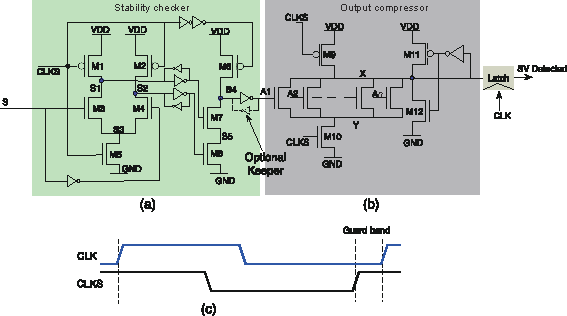
\includegraphics[scale=0.95]{fig1-2}
\caption{Timing sensor design. (a) stability checker; (b) output compressor; (c) clock timing.}
\label{fig:timing-sensor} 
\end{figure}


In symptom-based fault prediction, a symptom is defined as a signal stability violation. Basically, the stability violation of a signal is defined as at least one transition happens in the time interval during which the signal should be kept stable. A setup time violation, ascribed to progressive silicon aging for example, is a type of typical stability violation. As Fig. \ref{fig:timing-sensor}(c) shows, in a clock cycle, we should reserve a timing span, that is a safeguard band, to meet the minimal setup time requirement. For the degradation-free case, there should be no single transition during the safeguard band; By contrast, if the transistors involved on the relevant timing paths suffer sufficient aging, the transition-free condition can no longer hold. By detecting the transitions in the safeguard band, the impending faults can be detected. Of course, whether an aged circuit can result in a stability violation is determined not only by the “sickness” of the silicon, but also by the data patterns which can sensitize the corresponding timing paths. However, the timing paths of Sick Silicon will show a much higher probability than healthy silicon to trigger the stability violations. By detecting the distribution of the stability violation, we can discriminate the sick parts from the healthy parts. 

The key instruments to detect the stability violation is timing sensors, which are commonly based on dynamic circuits satisfying sub-nanosecond to even tens of picoseconds detection resolution. Fig. \ref{fig:timing-sensor} shows a sensor design. The basic stability checker (Fig. \ref{fig:timing-sensor}(a)) can be derived from a sensing circuit for on-line delay fault detection, in which the integrity of the signal (S) is verified by a pair of exclusive nodes (S1 and S2), a stability violation will discharge the charged node and thereby cause both nodes to be at the “0” state, which signifies a timing violation. The outputs are compacted with a dynamic NOR for reducing the number of output latches (Fig. \ref{fig:timing-sensor}(b)), where the M11 and M12 serve as a level restorer for node X. Multiple timing sensors are embedded in the host chip during fabrication. These sensors collectively form a monitoring system with fine-grained spatial detection resolution. The problematic component, such as an arithmetic logic unit (ALU), or a L1 cache bank, can be pinpointed. These faulty components can be masked from the other healthy parts, simply like a patient undergoes a surgery. These circuit-level adaptations can be automatically executed transparently on the host operation systems.

\subsection{Self-Diagnosis}
In on-chip fault tolerance, the diagnosis has two objectives: (1) pinpointing which components have been suffered permanent faults, and (2) estimating the level of performance degradation will be taxed due to the faults. Before delving into the details, we would like to first clarify the key differences between the built-in on-chip fault diagnosis and conventional chip diagnosis routines. The built-in on-chip fault diagnosis routine, called self-diagnosis, is very different from conventional diagnosis used in the yield learning phase, in terms of objective, techniques used, target granularity, and fault models.

\begin{itemize}
\item First, self-diagnosis is used to identify and locate the malfunctioning components, while the diagnosis in the production phase is mainly to help locate the defective physical or electrical contexts \cite{aitken2012yield}. The designers refine the physical designs to avoid these cases to ramp up the yield learning rate.

\item Second, the self-diagnosis intrinsically relies on built-in logic to locate the defective component, while the conventional diagnosis heavily relies on the silicon scan test and is conducted off-line by using sophisticated logical diagnosis tools.

\item Third, the granularity of self-diagnosis uses relatively coarse-grained components, such as core-level granularity, which have independent functionality and are usually loosely coupled with other parts, while the conventional diagnosis works at much finer-grained granularity at the logic gates or standard cells. In other words, self-diagnosis is based on functional testing and conventional diagnosis is based on structural testing.

\item Accordingly, the fault models of self-diagnosis describe the malfunction of components and therefore are more ad hoc, such as parity mismatch in the ALU components, while that of conventional diagnosis targets more silicon-level imperfections, such as bridge, open, abnormal leakage.
\end{itemize}

For on-chip fault tolerance, determining which parts of a chip get sick usually is trivial with the fine-grained self detection facility. If the corresponding timing sensors keep alerting stability violations, the faulty components can be switched off to avoid erroneous computations. In this case, the diagnosis and associated repairs are trivial. From Fig. \ref{fig:self-diagnosis-example}, for example, there are four homogeneous ALUs in the processor core, the diagnosis agent logs the number of alarms reported by the self-test procedure. Each logging period can be as long as days or weeks to improve the diagnosis confidence level. By analyzing the alarm distribution, the self-diagnosis agent can discriminate the faulty ALU. In this example, the alarm density ascribed to ALU2 is significantly higher than the others, so the diagnosis agent marks that ALU2 should no longer be available anymore. The computation is thereby offloaded to the remaining three health ALUs. Consequently, this core will continue to work at the degraded performance level. The similar diagnosis logic can be also applied in the core-level, especially for many-core processors.

\begin{figure}[t]
\centering
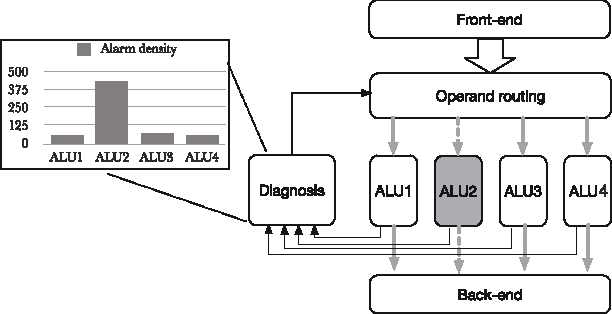
\includegraphics[scale=0.85]{fig1-3}
\caption{An self-diagnosis logic example for a 4-ALU processor.}
\label{fig:self-diagnosis-example} 
\end{figure}

It is more challenging to determine the performance impact given the faults detected, because the performance degradation depends on both the applications and the extent of the defects. For example, Fig. \ref{fig:performance-degradation} shows the performance responses of the cores under various types of degradation. The cores are salvaged from instruction window defects, or L1 instruction/data cache defects, or L2 cache defects, respectively \cite{powell2009architectural}. For simplicity, we do not show the more complicated compound defects. The degradation degree of “0” indicates defect-free, and 1/2 indicates half of the resource is unavailable, and so on. The results show that the performance response not only depends on the degree of degradation, but also exhibits to be highly application-specific. For example, the gobmk (a SPEC CPU2006 benchmark) in Fig \ref{fig:performance-degradation}(a) shows to be very resilient to the instruction window degradation; however, by contrast, the leslie3d and GemsFDTD are very sensitive to it. Such complexity is never unique for the instruction window only, but also to other resources, as exemplified in the other three sub-figures. Hence, even though the defect and associated defect level are accessible to the OS, we still have no ways to determine the level of performance impact such a degradation causes the running applications.

\begin{figure}[t]
\centering
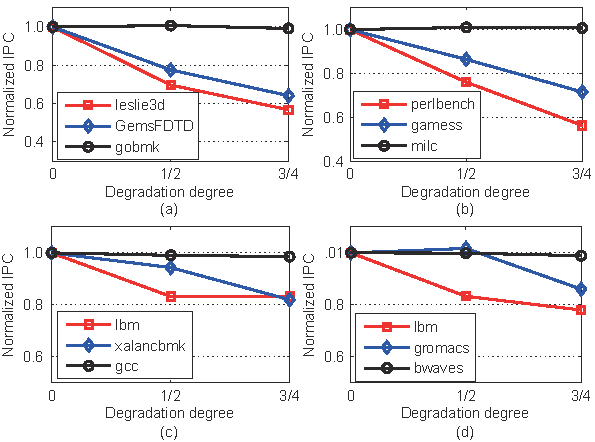
\includegraphics[scale=0.85]{fig1-4}
\caption{Performance degradation vs. defect degrees of (a) instruction window, (b) L1 instruction cache, (c) L1 data cache, (d) L2 cache, where the following SPEC CPU2006 benchmarks are used: leslie3d, GemsFDTD, gobmk, perlbench, gamess, milc, lbm, xalancbmk, gcc, gromacs, and bwaves.}
\label{fig:performance-degradation} 
\end{figure}


Yan et al. \cite{yan2015corerank} proposed the CoreRank approach to address this challenge. The CoreRank quantifies the core-level performance degradation towards more meta-program representations, called snippets, which are dynamic micro-operation streams and are oblivious to all the software level interference. The snippet can be readily characterized by built-in performance counters, without any instrumentation into the running workloads. The performance of core $C_i$ on the snippet $S_m$ is denoted as $P(C_{i}|S_{m})$, which can be obtained by reading the corresponding performance counters \cite{eyerman2007top}. If $P(C_{j}|S_{m})$ differs from $P(C_{i}|S_{m})$, the relative degradation can be easily extrapolated as the ratio of $P(C_{j}|S_{m})$ to $P(C_{i}|S_{m})$. Given any running program is composed of a sequence of various meta-programs (snippets), the program-level performance degradation can be estimated by aggregating the degradation on each individual snippet. Please refer to \cite{yan2015corerank} for more details.

For on-chip fault tolerance, the diagnosis is triggered only when the test procedure prompts the alarms. To minimize the overhead, one diagnosis agent can be shared by multiple timing sensors in a round-robin manner \cite{yan2011revivenet} controlled by a finite state machine. To minimize the penalty of power and performance in the fault-free scenarios, the diagnosis procedure is not always on, but is periodically invoked by abnormal states such as a machine crash.

\subsection{Self-Repair}
Generally there are two types of core-salvaging approaches: (1) Fault isolation. Decoupling the faulty components \cite{aitken2012yield} can avoid execution contamination and maintain a graceful degradation of performance. (2) Adaptive voltage-frequency setting and timing recycling \cite{tschanz201045nm}. For example, if the critical path delay increases due to aging, the functionality is maintained provided the working frequency is slowed down to accommodate the extra delay. The self-repair can be implemented at three abstract levels: circuit level, microarchitectural level, and architectural level. But we should note that such a classifying scheme is never strict, but only provides a roughly categorical image for easier understanding.

\subsubsection{Rejuvenation at the circuit level}
Fig. \ref{fig:circuit-repair} illustrates a circuit-level pipeline with a rejuvenation facility. Each stage is monitored by a set of periodically-invoked aging sensors used to detect the signal transitions in the safeguard band. The aging sensors are deployed to monitor the critical paths. In the fault-free scenarios, no transitions could happen in the safeguard band, but after suffering from aging, some transitions could be delayed into the safeguard band, represented as a stability violation \cite{yan2010svfd}, a type of faulty symptom. With the awareness of aging, we can accommodate the impending aging failures by adapting localized timings. The adaptation to each stage is implemented with a set of time-borrowing agents which are fed by not only the local stages aging sensors but also the next stages agents, thereby enabling bidirectional adaptation, namely backward timing adaptation (BTA) and forward timing adaptation (FTA). The BTA uses the $(K + 1)$st stages timing slack to accommodate the aging emergencies in the $K$th stage, while the FTA uses the $(K1)$st stages slack to accommodate the emergencies in the $K$th stage. When an aging sensor detects an alarm, the BTA, FTA, or BTA and FTA can be simultaneously enabled to tolerate this aging delay.

\begin{figure}[t]
\centering
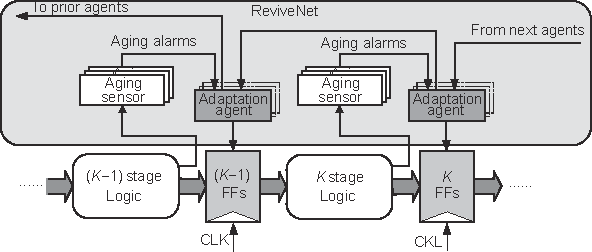
\includegraphics[scale=0.95]{fig1-5}
\caption{Circuit-level rejuvenation with timing adaptation.}
\label{fig:circuit-repair} 
\end{figure}


\subsubsection{Rejuvenation at the microarchitectural level}
The microarchitectural rejuvenation largely relies on decoupling the faulty components from the remaining healthy parts, or reconfiguring the microarchitectures \cite{powell2009architectural}. The components which can be readily modified to be reconfigurable include the ALU arrays, cache banks, and register files. They share the common feature of regularity with intrinsic spares. The repaired procedure is also similar: marking the faulty component as unavailable so it will never be allocated to dynamic instructions. With some more sophisticated circuit techniques, these components can even be totally decoupled from the power grid, thereby preventing them from leakage.

For example, as shown in Fig. \ref{fig:microarch-repair}, Core A and Core B suffered a pipeline defect and an L1 I-cache defect, respectively. The defect-affected partitions, marked as dark parts, are decoupled from the rest to make each core functionally correct, but in a degraded manner.

\begin{figure}[t]
\centering
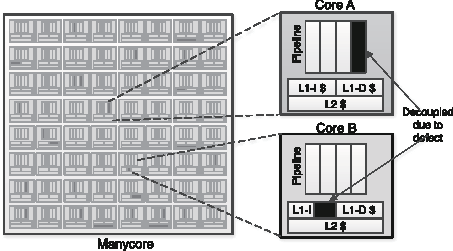
\includegraphics[scale=0.85]{fig1-6}
\caption{Microarchitectural rejuvenation.}
\label{fig:microarch-repair} 
\end{figure}

In fact, such microarchitectural approaches are more common in on-chip memory subsystems. A cache or scratchpad memory, always occupies a significant proportion of silicon real-estate. Using the last level cache for example as the failure mechanism in the SRAM cells, it suffers from different fault models, such as permanent read/write failures due to the SNR issue, retention fault or single-event upset (SEU). Regarding the granularity of the cache failures, it includes conventional bit failures and array or bank failures that occur in large-scale cache structures like distributed NUCA architectures. Fine-grained cache failures can be cured with conventional error correction or bit/row/column replacement. However, in modern large scale chip multi-processors, bank-level failures due to interconnection issue or isolation requirements are less discussed. For example, when a NoC-node is isolated from a resilient chip multiprocessor, it also creates inaccessible NUCA cache banks because of the connectivity issue, which should be tolerated to enable a degradable cache system. We propose a bank remapping method to cure the coarse-grained NUCA cache failure within the framework of self-test, self-diagnosis, self-fault-isolation. It utilizes the routing logic in Network-on-Chip to transparently remapping the physical space associated to failed banks to healthy cache banks, so that the system will not see the cache failure and maintain a wholesome physical memory space on-chip. 

Furthermore, to reduce the negative impacts imposed by the bank failures, our work uses a utility-driven remapping policy to match the failed cache banks to an under-utilized cache bank, so that the system receives the least performance penalties caused by the bank failures. The remapping method relies on a dynamic stack-distance analyzer to measure the space utility of different address spaces and keeps on remapping the failed banks to their favored compatible healthy banks. In this way, the bank sharing induced block conflict will be reduced and the conflict-induced eviction cache miss rate will be minimized. The whole framework guarantees that the bank failure will be tolerated with a very small performance cost. When future systems are built with unstable devices or an unstable environment, such an inexpensive fault tolerant mechanism is very useful.

\subsubsection{Rejuvenation at Architectural Level}
The architectural rejuvenation is usually conducted at the core-level. There are two major rejuvenation styles: topology-invariant and topology-reconfigurable approaches, where the topology refers to the NoC topology connection of tens even hundreds of cores. 

Using core level DVFS to tolerate a cores degradation is a typical topology-invariant approach. The cores initially have the same maximum frequency, Fmax, but with the in-field aging degradation, the Fmax of the cores can differ from each other. If a core ages with a prolonged critical path delay, we can scale down the cores frequency to maintain safe timing, at the expense of more sophisticated per-core DVFS. Meanwhile, the topology, that is the cores location related to other cores, remains intact. 

The topology-invariance can simplify the NoC implementation and traffic management. However, if a core suffers an irreparable failure, we must either map it out of the healthy region, or find a substitute. In either case, the topology must be changed and topology-reconfigurable approaches must be employed \cite{fu2011abacus} \cite{zhang2009topology}. One typical solution is called N +M paradigm, i.e., there are N normal cores, which are visible to the OS, and M spare cores, which only serve as substitutes for failed cores and are invisible to OS. The similar solution is adopted in the “Cell” processor (N=7, M=1), where an N-core processor is provided with M redundant cores and we always provide customers with N operational cores. The spare cores are viewed as overhead. However, as the number of on-chip cores increases, the overhead of leaving a few redundant cores on-chip unused is acceptable because a single core is inexpensive compared to the entire chip. 

In fact, the industry has started to employ core-level redundancy in their products. Even though the objective is mainly for yield or performance, a similar rationale should be also applied to enhance the lifetime reliability. In such a case, rejuvenation is about substituting the faulty cores with the spares. The topology determines the ideal performance whereas the routing algorithm and the flow control mechanism determine how much of this potential is realized. However, when the failure cores are replaced by spare cores, the topology of the target design can be different. For example, suppose we want to provide 9-core processors with a 3×3 2D-mesh topology, as shown in Fig. \ref{fig:topology-reconfig}(a). Also, suppose three redundant cores (1 column) are provided, as shown in Fig. \ref{fig:topology-reconfig}(b). If some cores (no more than three) are defective, we could still get 9-core processors. 
However, from Fig. \ref{fig:topology-reconfig}(c), if the faulty cores are replaced by the spare cores, not only are the topologies different from what we expect, but also the topologies of different chips can be very distinct. Consequently, there is a mismatch between the logical topology, 2D-mesh in this example, and the physical topology, namely the topology with the disabled cores. Clearly, there could be many ways to map the logical topology to the physical topology. So, the challenge in the N + M paradigm is to determine which topology is optimal. The problem has been proven to be NP-complete and can only be solved with a heuristic algorithm \cite{zhang2009topology}.

\begin{figure}[t]
\centering
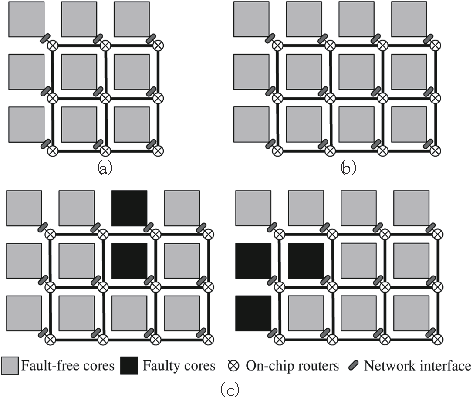
\includegraphics[scale=0.9]{fig1-7}
\caption{Topology reconfiguration-based architectural level rejuvenation for a manycore. (a) The topology demand;
(b) the topology with spare cores; (c) the topology with faulty cores.}
\label{fig:topology-reconfig} 
\end{figure}

\subsection{General Benefits}
The on-chip fault tolerance computing paradigm has great potential to critically complement the state-of-the-art IC designs. However, we should note that the specific techniques mentioned above should not be supposed to be comprehensive, but the concept of the 3S-based on-chip fault-tolerant design framework can be tailored for more purposes. We summarize three perspectives in the following section.

\subsubsection{Maintaining graceful degradation}
Faults could happen during the lifetime of a system. If the faults are transient, the system may be recovered by rebooting. However, if the faults are permanent, some resources of the system, such as cores in multi-core processor or interconnections of NOC will no longer be functionally correct. Without isolating the faults, the whole system may even turn off completely. However, by detecting, diagnosing, and isolating the faulty components, the system may still be able to work correctly using the remaining good components, though at a lower performance degree, i.e., Graceful Degradation. No redundant components are assumed, which means the components of the system have already satisfied the capability of reconfiguration for correct function. It is not surprising that these two design philosophies converge since they share the same objective. There are two key questions required to be answered for the on-chip fault tolerance computing paradigm based graceful degradation: (1) what is the granularity? (2) how to implement it? The on-chip fault tolerance computing paradigm sheds light on the answers.

The processor core and the NoC interconnection are two typical reconfigurable components used in graceful degradation. In multi-core processors, when one core is faulty, other cores can still function. In the NoC, when one interconnection node is faulty, other nodes may substitute its routing function. With on-chip fault tolerance, there are more redundant resources to keep the whole system working properly. More fine-grained components can also be considered. For example, a redundant arithmetic logic unit (ALU) can be added to a core, so when one ALU fails, the core can still work correctly.

Using more fine-grained components for fault tolerance and performance degradation can improve the lifetime of the system, but its disadvantage is the hardware cost, not only including the hardware for isolating the faulty components, but also including the hardware of detecting such fine-grained components. However, FPGA is an exception, since it is programmable. Hence detecting the faulty Look-Up tables (LUTs), interconnection boxes, or other fine-grained components of FPGA can be realized by specific circuits, and isolating the faulty resources can be achieved using placement and routing constraints while designing FPGA circuits. Hence, it is possible for FPGA to perform fine-grained analysis without any hardware overhead, but with a performance penalty.

Furthermore, on-chip fault tolerance computing paradigm provides more possibilities and opportunities for effective graceful degradation. The implementation of graceful degradation requires accurate diagnosis of the faulty components. For example, in NOC, it is necessary to diagnose the switch, the router, the link, and so on \cite{kohler2010fault}. With the knowledge of locating the faulty components, the routing for graceful degradation is an optimization process with the constraint that the faulty interconnections should not be used. With more faulty components, more constraints exist in the optimization problem, so its solution, i.e., the performance, will become progressively worse, until it reaches a limit that no available routing can be found, and then the whole system will fail. 
Moreover, on-chip fault tolerance computing paradigm can make the graceful degradation more simplified and effective. If an interconnection node has two routers, one of which is redundant, then when the working router fails, the node can simply switch to the redundant one. In this case, the routing delay remains similar, so the performance is maintained.

\subsubsection{Helping fix some verification blind spots}
Modern designs have become more complicated, which poses serious challenges for verification. The verification techniques cannot scale to the complexity of the modern designs, so some bugs could escape from verification and remain in the silicon. If the bugs really exist, they are like permanent faults. If these faults are not detected during testing, the products with bugs will enter the market. If the bugs are encountered by customers, it will be a large financial loss to recall the chips. In this situation, On-chip fault tolerance computing paradigm is an alternative method to fix the problem. On-chip fault tolerance computing paradigm has at least two benefits for verification: (1) locate the verification blind spots; and (2) fix the escaped bugs.

From the perspective of behavior, the escaped bugs are like permanent faults. Both cause the system to work incorrectly. In on-chip fault tolerance computing paradigm, the preliminary step for isolating faults is to detect and diagnose the faults. The same function is suitable for finding the escaped bugs. Learning how and why the bugs escaped from the adopted verification techniques is important for improving the verification process and avoiding the similar bugs remaining in silicon. A more fine-grained fault detection can provide more precise information about the escaped bugs. For example, it is easy for the designers to learn the escaped bugs by informing them just the ALU is faulty than informing them the whole processor core is faulty.

Therefore, the detection circuit for escaped bugs should be designed properly. For example, the detection circuits can be inserted in some critical points in the control flow \cite{gizopoulos2011architectures}. Within the on-chip fault tolerance computing paradigm, the faults are isolated to allow the whole system to work correctly. Some bugs can also be isolated. However, since the bugs may be repeated, isolating the bugs may not be effective. For example, in the multi-core processor, if all the cores have the same design, they will contain the same bugs as well, so it is meaningless to isolate faulty cores. 

Under this scenario, there are three ways to correct the bugs. First, heterogeneous cores can be designed so that even if one type of core contains bugs, other types of cores may still function correctly by isolating the faulty cores. But this method may result in a large performance losses, since a portion of the cores are unavailable. Second, during the design, combined with fine-grained bug detection circuits, some configurable components can be inserted into the critical locations \cite{alizadeh2010debugging}. If bugs are detected, specific configuration bits can be downloaded to the configurable components to correct the circuit behavior. Furthermore, in the CPU+FPGA SoC, if some bugs exist in the computing components, it is also possible to use the FPGA as a fault-tolerant component to perform the correct function. Third, for some bugs, it is also possible to use software-hardware cooperation to bypass the bugs \cite{chang2011constraint}. For example, if there is a bug in the subtraction computation hardware component, the OS can compile a subtraction operation into an add operation. In this way, the same function is performed by detouring the bugs. Therefore, using the above methods, with properly inserted bug detection and recovery design, some escaped bugs from the verification phase can still be fixed after the chips are manufactured and sold to the customers, though with some performance degradation.

\subsubsection{Improving gross yield}
Bugs may escape from verification, and defects may happen during manufacturing. There are mainly two types of defects: the permanent defect and the transient defect. The permanent defects such as stuck-at faults will permanently affect the behavior of the chip. More specifically, they destroy the Boolean relation within the chip. In certain situations, the chip or the corresponding component will definitely fail. The transient defects, such as small delay defects, are types of timing faults. The chip only fails under a certain condition. Different from bugs which may be repeated, e.g., in multi-core processors, the cores with the same design have the same bugs, the defects do not have such characteristics. Hence the on-chip fault tolerance computing paradigm can also tolerate some defects. The chips with defects are considered as faulty chips, but if the defects can be tolerated, then the chips can still work correctly and be considered as good chips. Hence, the yield can be improved, but the promised performance may be degraded.

\section{Summary}
The proposed on-chip fault tolerance computing paradigm is an incorporative framework to build synergy among many advanced fault tolerance-oriented techniques. In this paper, we placed self-test, self-diagnosis, and self-repair (self-recovery) into a unified framework, namely the “3S” framework, and clarified the difference from their conventional counterparts whenever possible. We use the manycore undergoing various degrees of aging faults as the baseline to show the efficacy of on-chip fault tolerance, and discuss three far-reaching implications in terms of graceful degradation, verification, and yield. Although we have made some initial attempts to solidify this framework, the potential has never been fully exploited. We believe on-chip fault tolerance can help deliver more reliable SoC systems suffering in-field degradation in the future.

\bibliographystyle{plain}
\bibliography{refs}



%%%%%%%%%%%%%%%%%%%%% chapter.tex %%%%%%%%%%%%%%%%%%%%%%%%%%%%%%%%%
%
% sample chapter
%
% Use this file as a template for your own input.
%
%%%%%%%%%%%%%%%%%%%%%%%% Springer-Verlag %%%%%%%%%%%%%%%%%%%%%%%%%%
%\motto{Use the template \emph{chapter.tex} to style the various elements of your chapter content.}
\chapter{Fault-Tolerant Circuits}

\abstract{
The aggressive technology scaling poses serious challenges to lifetime reliability. A parament challenge comes from a variety of aging mechanisms that can cause gradual performance degradation of circuits. Prior work shows that such progressive degradation can be reliably detected by dedicated aging sensors, which provides a good foundation for proposing a new scheme to improve lifetime reliability. In this paper, we propose ReviveNet, a hardware-implemented aging-aware and self-adaptive architecture. Aging awareness is realized by deploying dedicated aging sensors, and self-adaptation is achieved by employing a group of synergistic agents. Each agent implements a localized timing adaptation mechanism to tolerate aging-induced delay on critical paths. On the evaluation, a reliability model based on widely used weibull distribution is presented. Experimental results show that, without compromising with any nominal architectural performance, ReviveNet can improve the Mean-Time-To-Failure by up to 48.7 percent, at the expense of 9.5 percent area overhead and small power increase.}

\section{On-line Fault Detection}
In ultra-deep submicrometer technology, soft errors and device aging are two of the paramount reliability concerns. Although many studies have been done to tackle the two challenges, most take them separately so far, thereby failing to reach better performance-cost trade-offs. To support a more efficient design trade-off, we propose a unified fault detection scheme—stability violation-based fault detection (SVFD), by which the soft errors (both single event upset and single event transient), aging delay, and delay faults can be uniformly dealt with. SVFD grounds on a new fault model, stability violation, derived from analysis of signal behavior. SVFD has been validated by conducting a set of intensive Hspice simulations targeting the next-generation 32-nm CMOS technology. An application of SVFD to a floating-point unit (FPU) is also evaluated. Experimental results show that SVFD has more versatile fault detection capability for fault detection than several schemes recently proposed at comparable overhead in terms of area, power, and performance. 

\subsection{Challenges for On-line Fault Detection}

The advancement of the semiconductor technology in the following decade will bring a broad set of reliability challenges at a dramatic fast pace \cite{sematech03}. Two of the paramount challenges are soft errors and aging-driven lifetime reliability. Many researchers focused on soft error modeling and mitigation within a wide design spectrum: device level, circuit level \cite{Mitra_C05}\cite{Han_DT05}\cite{Zhang_TVLSI06}, microarchitecture level \cite{Vijaykumar_ISCA02}, and software level \cite{Oh_TR02}. In addition, the industry and academic communities have done much work on understanding the semiconductor device reliability failure mechanisms and models, such as Electromigration \cite{Electromigration_69}, negative bias temperature instability (NBTI) \cite{NBTI_Impact05}\cite{Modeling-and-minimization_06}\cite{wang2007impact}, time dependent dielectric breakdown (TDDB), hot carrier injection (HCI), temperature cycling \cite{failure_models_00} etc.

Aging failure prediction \cite{agarwal2007circuit} \cite{failure_prediction2_08} is a promising approach to cope with aging effects. Unlike soft errors, device aging is a gradual process, which makes the prediction of aging degree achievable. Before the devices totally breakdown and thereby loss their functionalities, they always tend to exhibit performance degradation, e.g. increased threshold voltage instability, soaring leakage power, worse heat characteristics etc. Most of these negative effects can result in the degradation of switch performance of the transistors\cite{degradation_05}, and eventually excessive path delay. In other words, most of the aging failures can be predicted by sensing the gradually increased aging delay. Agarwal et al. designed an aging sensor for this purpose \cite{agarwal2007circuit}.

On the other hand, semiconductor devices are becoming increasingly prone to soft errors (SEUs and SETs) as feature size decreases \cite{Shivakumar_DSN02}. Abundant redundancy design solutions have been proposed to combat the soaring soft error rate, such as spatial redundancy by duplicating the flip-flops \cite{Mitra_C05} \cite{lowcost_date07}, or temporal redundancy by multiple-sampling \cite{Nicolaidis_VTS99}. Even if the overhead imposed by these redundancy can be kept in check, these "redundancy" resources, however, help little in mitigating aging effects, and in contrast even speed up the aging process due to the extra heat generated by those redundancy resources. This dilemma makes the goal of providing a not only aging-resistant but also soft error-tolerant scheme hard to achieve, unless a cumbersome combination of the previous aging-sensor and redundancy-based approaches is conducted.

Rather than attempting to exploit such a cumbersome combination, in this paper, we propose a unified mechanism to face the two challenges. Based on signal behavior analysis, we find that the soft errors and aging delay can converge into the same signal behavior: \emph{Stability Violation} to the target circuits. Even the conventional delay faults, which could result from such as transition hazard, crosstalk, can be represented as stability violations. Hence, it is promising to propose a unified fault model and associated detection mechanism, thereby creating the chance of reaching a more optimum trade-off between detection capability, design complexity, and implementation overhead. To our knowledge, this is the first work to handle the soft errors, aging delay, and delay faults under a unified fault detection mechanism.

\subsection{Stability Violation Based Fault Detection}

The stability violation of a signal is defined as at least one transition happens in the time interval during which the signal should be kept stable. Setup time violation, which the progressive aging delay tends to contribute to, is a typical example of stability violation. Apparently, only coping with setup time violation is far from sufficient to handle soft errors and delay faults. In the rest of this Section, we will present how to comprehensively describe the rationale behind stability violation, and meanwhile how to generalize it to propose a unified fault model.

First, we specify the target fault types, and then move to the unified stability violation model and associated SVFD mechanism.

\subsubsection{Target Fault Types}
{\bf Soft Error:} \emph{Single Event Upset} (SEU) and \emph{Single Event Transient} (SET) \cite{Nicolaidis_TDMR05}. If some high energy radioactive particles induce a storage cell to be flipped, this unintentional bit-flip is called SEU. If the particles cause a node of combinational logic to collect enough charge, a transient current pulse could be generated. This pulse can transform into a voltage pulse and propagate along logic paths  \cite{Shivakumar_DSN02}. This type of soft error is called SET. A soft error might not be captured by flip-flops due to three masking effects \cite{Shivakumar_DSN02}: Logic Masking, Electrical Masking, and Latching-window Masking.

{\bf Aging Delay:} The aging effects, such as NBTI, can cause aging delay which can be used for aging-failure prediction\cite{agarwal2007circuit}. Usually, the aging delay increasing is a gradual process over time, though the abrupt delay increasing is possible when the devices suffer from breakdown induced by mechanical stresses. This type of "abrupt" aging delay will not be covered in this paper.

{\bf Delay Fault:} This type of faults refers to the conventional delay faults \cite{favalli1996sensing} which is caused by device defect, signal crosstalk, etc. This
paper handles the delay faults with size less than the width of the Detection Slack.

\subsubsection{Modeling Faulty Signals}
Mathematically, a signal $S$ can be expressed as a function of time $t$, expressed as $S = f(t)$. Given the time interval of $(t_i, t_t)$ in which $S$ gets into a stable state before $t_t$, this interval can be divided into two periods: \emph{variable period} denoted by $T_{vp}^S=(t_i,\;t_{s})$, and \emph{stable period} by $T_{sp}^S=(t_{s},\;t_{t})$, where $t_{s}$ is the complete time of the last transition of $S$ within the specified interval. In addition, the initial value and the terminal value of the signal are expressed as $F_i^S = f(t_i)$ and $F_t^S=f(t_t)$, respectively.

According to the above definition, we define a faulty signal, $S_f$, that commits at least one of the three violations:
\begin{itemize}
  \item Initial Value Violation (IVV): The obtained value of $F_i^{S_f}$ at time $t_i$ differs with
   $f(t_i)$.
  \item Terminal Value Violation (TVV): The obtained value of $F_t^{S_f}$ at time $t_t$ differs with
   $f(t_t)$.
  \item Stability Violation (SV): One or multiple transitions happen in the stable period.
\end{itemize}


The above violation behaviors, strictly speaking, can not precisely capture all details of signal mismatch between a fault-free signal and its faulty counterpart; However, the above violation definitions are actually robust enough to guide high efficient on-line fault detection, as the following presents. In fact, given the target fault types including soft errors, aging delay, and delay faults, only the stability violation of a signal is needed to be verified. The following explains how to use this model in a practical way.

First, the variable period $T_{vp}$ and stable period $T_{sp}$ for a specified signal need to be established. Figure \ref{comb} models a general logic circuit. The input signal $S_i$ comes from the upstream flip-flop, and the output $S_o$ is captured by the downstream flip-flop. Both flip-flops are synchronized by the same clock $clk$ with cycle period of $T$. Several timing parameters are summarized below:
\begin{itemize}
    \item $t_{pd}$:  the  propagation delay of the combinational logic;

    \item $t_{cd}$:  the  contamination delay (a.k.a. short-path delay) of the combinational logic;

    \item $t_{cq}$: the flip-flop's  clock-to-q time.
\end{itemize}

\begin{figure}[t]
\centering
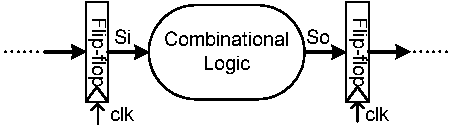
\includegraphics[width=0.4\textwidth]{fig2-1}
  \vspace{-0.5em} 
  \caption{Generic logic circuit}
  \label{comb}
\end{figure}

The $S_i$ gets updated only at every effective clock transition and is held for the whole cycle period, which means almost no variable period exists. Thus the variable period, and the stable period of $S_i$ in the $n^{th}$ clock cycle $((n-1)T, nT)$ can be expressed as:
\begin{align}
%F_{s}^{S_i}&=f_{s_i}((n-1)T+t_{cq}) \label{Sivs}\\
T_{vp}^{S_i}&=((n-1)T, \;(n-1)T+t_{cq}), \\
T_{sp}^{S_i}&=((n-1)T +t_{cq}, \;nT).
\end{align}

The variable period of $S_o$, unlike that of $S_i$, is much more prominent; the $S_o$'s  variable period and stable period in the $n^{th}$ clock cycle can be expressed as:
 \begin{align}
%F_{s}^{S_o}&=f_{s_o}((n-1)T+t_{cq}+t_{pd})\\
T_{vp}^{S_o}&=((n-1)T+t_{cq}+t_{cd},\; (n-1)T+t_{cq}+t_{pd}) \\
T_{sp}^{S_o}&=((n-1)T+t_{cq}+t_{pd},\; nT+t_{cq}+t_{cd}) \label{SoSP}
\end{align}

Figure \ref{tvts} illustrates the time periods of both $S_i$ and $S_o$ in the $n^{th}$ cycle, where $t_{1}=(n-1)T+t_{cq}+t_{cd}$, $t_{2}=(n-1)T+t_{cq}+t_{pd}$.

\begin{figure}[ht]
\centering
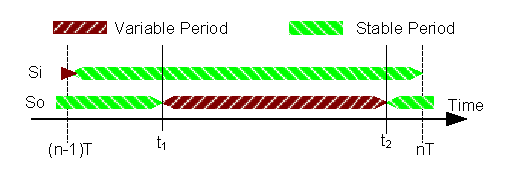
\includegraphics[width=0.5\textwidth]{fig2-2}
   \vspace{-0.5em}
   \caption{Variable Period VS. Stable Period}
   \label{tvts}
\end{figure}

With the defined time periods, we can explain how the target faults commit the above violations and, what's more, how these IVV and TVV converge to SV.

1) Suppose that a delay fault occurs, the delayed $S_o$ will cause SV in Detection Slack ($T_{DS}$) during which the $S_o$ should keep stable. Equivalently, the delay fault will result in $S_o$'s TVV since at the end of the cycle, $S_o$ can not reach the expected value. This TVV then causes the IVV of the signal in the next stage of logic. Hence, SV, TVV, and IVV are equivalent to each other for the delay fault.

2) Suppose that an aging delay occurs, the delayed $S_o$ will cause SV in Guard Band ($T_{GB}$). Unlike the delay fault, the progressive aging delay will not cause TVV and IVV; therefore, an aging delay just represents as SV. Here the aging induced SV actually is quite similar to setup time violation.

3) Suppose that an unmasked SEU strikes the upstream flip-flop. Clearly, the $S_i$'s SV is committed because, after transient clock-to-q time, $S_i$ is supposed to keep stable during the whole cycle period. This SV could also potentially cause the downstream flip-flop to capture faulty data, and thereby results in $S_o$'s TVV, then IVV of input signals in the next stage logic. So, the SEU will represents as SV, and possible IVV and TVV.

4) Suppose that an unmasked SET happens in the combinational logic. If the duration of the SET is less than $T_{DS}+T_{GB}$, the behavior of the SET fault is similar with the commonly referred delay faults: unexpected signal transitions within the $S_o$'s stable period. Therefore, the analysis result for the delay faults also holds for SET faults. That is SV, TVV, and IVV are equivalently to each other for the SET.

From the above analysis we conclude that, from the signal behavior perspective, the target faults either induce equivalent SV, IVV, and TVV (for delay fault and SET), or only represent as SV (for aging delay), or SV and possible equivalent IVV and TVV (for SEU). In other words, the target faults can be uniformly modeled as SV. The implication is that we can employ a unified stability checker to handle the detection for all of the target faults. This unification can potentially support a more efficient implementation of the online fault detection scheme than the traditional redundancy-based approaches such as \cite{Mitra_C05}\cite{Han_DT05}. In addition, the capability for aging failure prediction \cite{agarwal2007circuit}\cite{failure_prediction2_08} can be exploited in place with the same scheme; thereby greatly facilitating the aging-aware designs.

\subsection{Timing Constrains Exploration}
The object of SVFD in essence is to distinguish those transitions violating the signals' stability specification from normal signal transitions, thereby achieving the goal of fault detection. The detection of SV can be accomplished with some kind of stability checkers.

\subsubsection{Propagation of Stability Violation}
The stability checkers are usually implemented with dynamic circuit style. So, the first concern is how to schedule the precharge period. Neither the traditional cycle-begin precharge (using the first half cycle period to precharge) nor cycle-end precharge (using the second half cycle period to precharge) styles are applicable in our detection mechanism. As Section III.B explained, during the \emph{Guard Band} and \emph{Detection Slack}, the checker should be on duty, instead of staying in precharge state. Given $S_o$ with prominent variable period, the precharge can be scheduled in the variable period. However, the same schedule strategy is unallowable for $S_i$ because there is almost no any variable period can be exploited for precharge. If we "brutally" borrow some time from $S_i$'s stable period for precharging the checker, the fault coverage has to be sacrificed.

To address this problem, we find if the precharge stage is scheduled according to some specific timing requirements, the fault coverage will not be compromised. The discussion about timing manipulations can be started with describing a key observation, called {\bf Propagation of Stability Violation}.

Suppose that an unmasked SEU occurs in an upstream flip-flop at time $t$ in the $n^{th}$ cycle, then the effects of the SV of $S_i$ should be propagated to $S_o$ within the time interval of $(t+t_{cd},\;t+t_{pd})$.  If the effects of $S_i$'s SV can propagate into $S_o$'s stable period, that is

\begin{equation}\label{precharge}
(t+t_{cd},\;t+t_{pd}) \subset (nT-T_{GB}, nT+T_{DS}), 
\end{equation} 

Then the SEU induced $S_i$'s SV can be represented as $S_o$'s SV since the $S_o$ should keep stable during the \emph{Guard Band} and \emph{Detection Slack}. Hence, the checker deployed to detect $S_o$'s SV can indirectly handle a part of $S_i$'s SV within a particular time interval, referred to {\bf Propagation Detectable Period (PDP)}. From (\ref{precharge}), we have

\[
\left\{
\begin{array}{ll}
 t+t_{cd} > nT-T_{GB}, \\
 t+t_{pd} < nT+T_{DS}.
 \end{array} \right.
\]

Then, the PDP can be expressed as

\begin{equation} \label{eq2}
\{t\,|\, nT-T_{GB}-t_{cd} < t <nT+T_{DS}-t_{pd}\}.
\end{equation}

\subsubsection{XOR Protection}

Not all unmasked SEUs occurring in the upstream flip-flop can translate into the $S_o$'s SV; for example, if a  $S_i$'s SV happened during the $((n-1)T,\; t_1)$ (Figure \ref{tvts}), then it could not be detected by $S_o$'s checker  because (\ref{precharge}) dose not hold in such case.

To cover this period, one way is to set another stability checker for $S_i$, at the expense of almost doubled area and power overhead. In contrast, we propose a simple but far more efficient way to cover this period, referred to \emph{XOR Protection}, as Figure \ref{xor} shows. The effectiveness of this scheme is based on the observation: the $S_o^{(K-1)}$ is consistent with the $S_i^K$ within the period of $((n-1)T,\; (n-1)T+t_{cq}+t_{cd})$; therefore, one XOR (or NXOR) gate is capable of capturing any $S_i^K$ stability violation during this span of time. The overhead imposed by an XOR gate is much less than that imposed by another stability checker or other traditional redundant flip-flop based schemes \cite{Mitra_C05}. How to efficiently handle the output of XOR will be presented in next Section.

\begin{figure}[t]
\centering
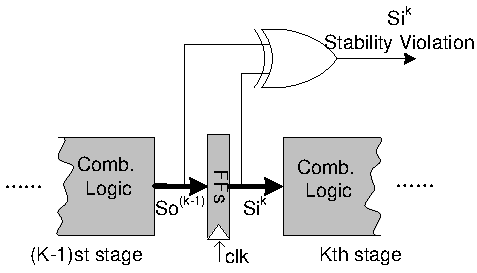
\includegraphics[width=0.45\textwidth]{fig2-3}
\vspace{-0.5em}  
\caption{XOR Protection}\label{xor}
\end{figure}

\subsubsection{SEU Detection "Blind Zone"}

The above timing constrains are still not comprehensive without taking another time interval called "blind zone" into account.  Considering the propagation delay of a SEU, we can claim that the SEU must be benign if

\begin{equation}\label{benign}
t>nT-t_{cd}.
\end{equation}

\begin{figure}[ht]
\centering
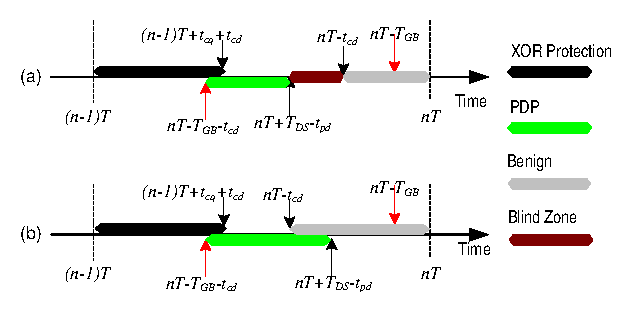
\includegraphics[width=0.6\textwidth]{fig2-4}
  \caption{Variety of timing period for $S_i$}\label{zones}
\end{figure}

To protect $S_i$ (from SEUs), besides the XOR protection period, the PDP, and the benign period, there might be the fourth region that has not be covered so far. Figure \ref{zones} shows that the whole Stable Period of $S_i$ could be divided into four or three zones, depending on different timing parameters. Specifically, Figure \ref{zones}(a) shows if $nT+T_{DS}-t_{pd}<nT-t_{cd}$, then a SEU occurring in the interval of ($nT+T_{DS}-t_{pd},\;nT-t_{cd}$)  may fail to propagate into the detectable period, thereby resulting in detection "Blind Zone". Unlike the XOR protection period, this trouble can not be eliminated unless another dedicated stability checker is set for $S_i$, at considerable expense of implementation overhead. Fortunately, we propose a new approaches: Contamination Delay Optimization, by which the ``Blind Zone" can be eliminated by some timing manipulations.

\noindent{\bf Contamination Delay Optimization:} Clearly, the "Blind Zone" can be naturally
eliminated if

\begin{equation}\label{ebz}
nT-t_{cd} < nT+T_{DS}-t_{pd}
\end{equation}

is satisfied, as Figure \ref{zones}(b) illustrates. The SEU happening in $(nT-T_{GB}-t_{cd}, \; nT+T_{DS}-t_{pd})$ is either propagated into a Stability Violation detectable zone of corresponding $S_o$, or has nothing detrimental effect due to residing in benign period. From (\ref{ebz}), we derive the contamination delay should meet 

\begin{eqnarray}\label{eq80}
 t_{cd} > t_{pd} - T_{DS}
\end{eqnarray}

In addition, given that the terminal time of XOR protection zone should meet

\begin{equation}
  nT-T_{GB}-t_{cd} < (n-1)T + t_{cd} + t_{cq}; \nonumber
\end{equation}

otherwise another "blind zone" would emerge; thus, we have

\begin{equation}\label{eq81}
  t_{cd} > \frac{1}{2}(T-T_{GB}-t_{cq}).
\end{equation}

Lastly, considering  $T_{DS}<t_{cq}+t_{cd}$ should always holds, that is
\begin{equation}\label{111}
  t_{cd}>T_{DS}-t_{cq}.
\end{equation}

From (\ref{eq80}), (\ref{eq81}), and(\ref{111}), we derive that $t_{cd}$ should meet the requirement:

\begin{eqnarray}\label{eq82}
  t_{cd} >  \max \{t_{pd} - T_{DS},\; \frac{1}{2}(T-T_{GB}-t_{cq}),\; T_{DS}-t_{cq}\}
\end{eqnarray}

Generally, (\ref{eq82}) requires the contamination delay of the combinational logic reaches up to about a half cycle period. The same requirement is needed to be satisfied in some previous studies \cite{lowcost_date07} to address "short path effects" \cite{Nicolaidis_ITC07}. Actually, It is consistent with the goal of many timing optimization strategies \cite{Delay_Insertion_06}\cite{Padding_93}, and therefore not a substantial limitation.

\subsubsection{Available Precharge Period}
Figure \ref{zones}(b) sheds light on when the precharge can be scheduled: within $(nT-T_{GB}-t_{cd},\; nT-T_{GB})$ the precharge can be conducted without sacrificing fault coverage. Additionally, to avoid the precharge intruding Detection Slack, the actual available start point of the precharge stage should be

\begin{eqnarray}\label{eq5}
\max\{nT-T_{GB}-t_{cd},\;(n-1)T+T_{DS} \};
\end{eqnarray}

therefore, the available precharge period is

\begin{equation}\label{prechargeperiod}
(\max\{nT-T_{GB}-t_{cd},\;(n-1)T+T_{DS} \},\; nT-T_{GB}).
\end{equation}

From (\ref{prechargeperiod}), the available precharge duration $\tau$ can be calculated by

\[\label{tao}
\tau = \left\{
\begin{array}{ll}
 t_{cd} & \mbox{if } t_{cd}<T-T_{GB}-T_{DS}, \\
 T-T_{DS}-T_{GB} & \mbox{otherwise}.
 \end{array} \right.
\]

To sustain normal operations, there is a minimum precharge duration $\tau_0$, which is determined by the intrinsic $RC$ constant. Clearly, $\tau > \tau_0$ needs to be satisfied. It is not difficult to meet this requirement. Experimental results show that for 65nm CMOS, 1GHz, $\tau_0$ is merely 40ps, while $\tau$ is at the magnitude of hundreds of picoseconds. More detail can be found in next Section.

To sum up, we can use only one stability checker, with the assistant XOR protection, for soft errors, aging delay, and delay faults detection for $S_i$ and $S_o$. All we have to do is to ensure (\ref{eq82}) and (\ref{prechargeperiod}).

As the end of this section, the following exemplifies an empirical analysis of the above constrains.

\vspace{0.3cm} {\bf Example.} Generally, $T_{DS}$ is determined by the maximum width of SET pulses, commonly conservatively being set to a half cycle period, that is $T_{DS}=0.5\times T$. $T_{GB}$ originally is determined by the aging detection interval---the time interval between two aging detection action (the aging sensor does not need to be always on).  $T_{GB}$ is much larger than 5\% of cycle period, as suggested by \cite{agarwal2007circuit}, but should be less (or not much larger) than the reserved timing margin. Since commonly 10\% timing margin is reserved to combat PVT variations, the cycle period dose not need to be increased to reserve extra time margin for $T_{GB}$. The propagation delay $t_{pd}$ hence is $T\times(1-10\%)=0.9T$. We omit the term of $t_{cq}$ because comparing with other timing parameters, $t_{cq}$ is marginal. Then, based on (\ref{eq82}) we need to figure out the minimal $t_{cd}$ since smaller $t_{cd}$ implies that smaller compensation effort and associated area overhead to pay. We suggest use the results: $t_{cd}=0.45T$, $T_{DS} = 0.45T$, $T_{GB}=0.09T$ because this configuration is competent enough in detecting SET faults, delay faults, and aging delays with modest compensation effort.

\subsection{On-line Fault Detection Architecture}
Figure \ref{imple}(a) shows the top view  of the whole fault detection scheme. Note that the XOR (NXOR actually) output needs to be gated outside of the XOR protection period where an XOR-flagged alarm can unintentionally discharge the detection unit if leave un-gated. The detailed timing relations and associate clock configurations is shown in Figure \ref{imple}(b), where CLKS is used to control precharge-evaluation, and CLKG is the gating clock for XOR output.

\begin{figure}[t]
\centering 
\subfigure[Top view of SVFD scheme]
{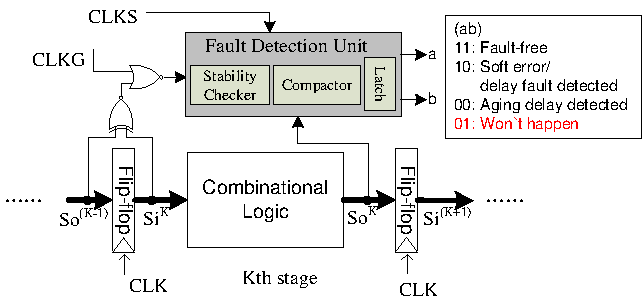
\includegraphics[width=0.6\textwidth]{fig2-5a}} 
\subfigure[Timing of precharge clock and XOR-protection gating clock]
{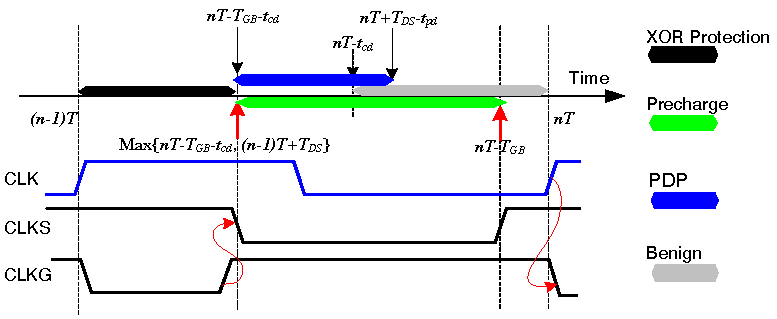
\includegraphics[width=0.7\textwidth]{fig2-5b}}  \caption{Top view of implementation}
\label{imple}
\end{figure}
\subsubsection{Circuit Design}
Figure \ref{circuit} shows the transistor level design of SVFD scheme. A detection unit consists of two key components: a stability checker (Figure \ref{circuit}(b)) and an output compactor (Figure \ref{circuit}(c)).

\begin{figure}[t]
\centering
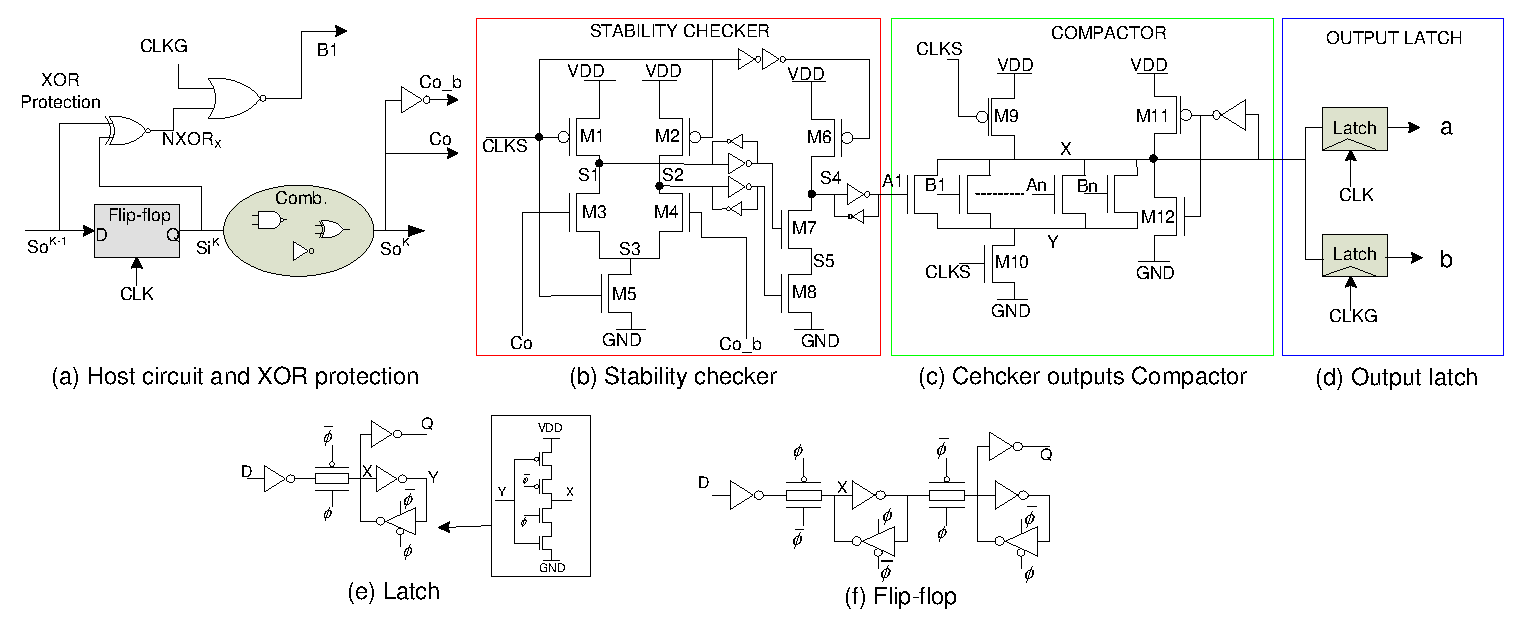
\includegraphics[width=0.95\textwidth]{fig2-6}
\vspace{-0.5em}  
\caption{SVFD Implementation} \label{circuit}
\end{figure}

The basic stability checker can be derived from a sensing circuit for on-line delay fault detection \cite{favalli1996sensing}, in which the signal integrity is verified by a pair of consistent charge/discharge nodes, a delay fault will trigger one of the nodes to be discharged/chargeed and thereby causes states inconsistent between them. The same fundamental detection principle is employed to design a sensor dedicated for aging prediction, referred as Aging Resistant Stability Checker (ARSC) \cite{agarwal2007circuit}. Based on the same principle, we design a new stability checker. Compared with ARSC, the checker has several new features which can improve the robustness and reduce the overhead. The following explains how does the circuit work and then presents the new features.

During precharge period, both nodes $S1$ and $S2$ in the stability checker are charged up to HIGH. Then, the circuit starts evaluation, one of the two nodes is pulled down, while the other one floats at HIGH because the gate signal of M3 is always complemented with that of M4 (a weak keeper can help the floated node stick to HIGH). Hence, the node $S1$ and $S2$ are always exclusive during fault-free time, which will make the node $S4$ stick to HIGH because the high-impedance path between S4 and GND always exists. When a Stability Violation is committed by $S_i$ (out of the XOR protection period) or $S_o$, the violation will trigger the discharge of the node that has charged up to HIGH. Eventually both nodes are discharged, and thereby the node S4 is pull down to LOW. Then, the node X in output compactor will be discharged, which flags a fault being detected. The compacted result X needs to be latched twice: CLK-latched for indicating aging delay and CLKG-latched for indicating soft error or delay fault (Figure \ref{circuit}(d)). The reason will be explained in Section VIII.

\begin{figure}[t]
\centering \subfigure[XOR Tree] {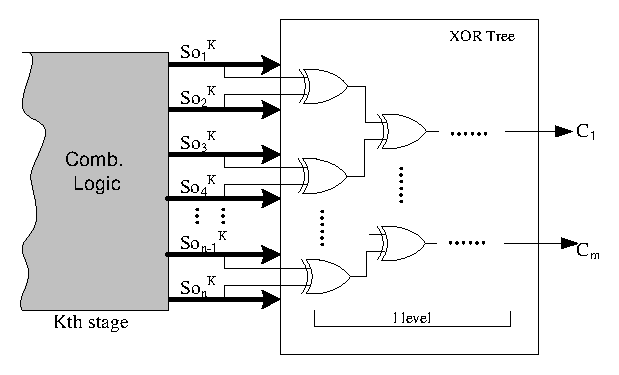
\includegraphics[width=0.55\textwidth, height=0.33\textwidth]{fig2-7a}}
\hspace{1cm} \subfigure[AND Tree]
{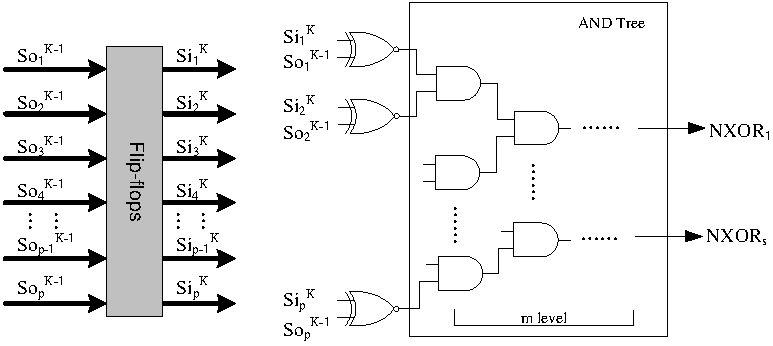
\includegraphics[width=0.7\textwidth,height=0.35\textwidth]{fig2-7b}}  \caption{Compacting the
output signals and XOR-protection signals} \label{compactor}
\end{figure}


There are two new features in the detection unit:

1) The NOR logic for combining the states of S1 and S2 is realized with a dynamic
logic (M6, M7, and M8), which can improve the robustness of the checker and reduce
the area overhead and switch power dissipation. Unlike the stability checker in ARSC
\cite{agarwal2007circuit}, where the checker output, a static NOR gate, is
directly driven by a floated HIGH node during fault-free time, our checker's output
is generated by a dynamic NAND gate. This change is based on that both the node S1
and S2 are pulled up to HIGH during precharge, and consequently both M7 and M8 are
turned off; thereby no short path existing when precharge. So the foot transistor
for the dynamic NAND is eliminated. Note that due to the precharge RC delay of S1
and S2, the M6's precharge clock should be delayed by a precharge delay constant to
avoid transient shot current in the NAND gate.

2) The outputs are compacted with a dynamic NOR for reducing the number of output
latches. Usually, it is not necessary to identify which signals commits the SV for
most aging-aware and fault tolerant designs. So the distributed detection results
can be ``compacted" to reduce the number of output latches. We use a wide dynamic
NOR to implement the compactor, in which the M11 and M12 serve as a level restorer
for node X.

%The fault detection is for providing fail-stop support or some on-line adjustments. While, so far,
%the fault detection can detected the fault at fine-grained: signal. This grained of fault
%detection is unnecessary, especial in the situation where the chips have been shipped to the
%customers.

%In addition,
%%this detection unit can be easily disabled by pulling up the CLKS to HIGH. The PMOS
%%transistor's aging process induced by NBTI effects is greatly slow down in disable
%%mode.
%unlink ARSC where the Guard Band is confined by a clock and its delayed counterpart
%\cite{agarwal2007circuit}, SVFD unit provides Guard Band by the  CLK and CLKS. So
%the clock skew needs to be controlled well. This issue is beyond the scope of this
%paper.


\subsubsection{Low-Overhead Deployment}
Given a target circuit, each output signal $S_o$ needs to be monitored by a
stability checker whose output is fed to a compactor, as Figure \ref{imple}(a)
shows. In addition, each XOR-protected signal gated by CLKG is also fed to a
compactor.   We present two deploying techniques to reduce the overhead coming from
the checkers, compactors, and latches.

\textbf{Compacting $S_o$ using XOR-Trees:} With XOR-Trees, we can enable checker-sharing mechanism among multiple output
signals, as Figure \ref{compactor}(a) shows, thereby reducing the number of
checkers. The rationale behind the XOR-Trees based compactor is the fact that for a XOR gate the non-simultaneous transitions of inputs can result in output transitions. This can be explained with the following example:

Suppose there are two signals $S_a$ and $S_b$, and signal $C = S_a \mbox{XOR} S_b$;
clearly, one or two non-simultaneous transitions of $S_a$ and $S_b$ can be exactly represented as or or two transitions of $C$. This fact implies that if $S_a$ or $S_b$ imposes stability violations, then $C$ must commit stability violations, too.

One side effect of XOR-Trees is that the compactor may hide some faults that happen to induce simultaneous transitions on the primary inputs of a XOR-Tree. For example, if $S_a$ happens to switch from HIGH to LOW, while at the same time $S_b$ from LOW to HIGH, then  $C$ may keep staying at HIGH. Fortunately, the possibility of such negative cancelation effect can be minimized by separating the $S_o$ from the same logic cone to different XOR-Trees, since it is rare for multiple faults happen in the same spot at the same time, especially for soft errors.

Figure \ref{compactor}(a) illustrates an application of a set of XOR-Trees which compacts $n$ output signals $So_1^K, So_2^K,\ldots, So_n^K$ into $m$ checker-monitored signals $C_1, C_2, \ldots, C_m$. We have 

\begin{equation}
m=\frac{n}{2^{\,l}}.
\end{equation}

The number of required XOR-gate used to implement an XOR-Tree can be easily calculated by

\begin{equation}\label{nxor}
  N_{xor}=n\times (1-(1/2)^{\,l}).
\end{equation}

%\begin{figure}[t]
%\centering
%\includegraphics[width=0.4\textwidth]{xortree.eps}
% \caption{XOR Tree}\label{xortree}
%\end{figure}

\textbf{Compacting $S_i$  using AND-Trees:} The similar strategy can be used to compact the XOR-protection results with AND-Trees. If one or more SEUs strike the set of flip-flops, then corresponding inputs of the set of AND-Trees will be pulled down to LOW, and then pull down the outputs of corresponding AND-Trees, denoted by NXORx in Figure \ref{compactor}(b).

Unlike XOR-Trees for compacting output signals, AND-Trees won't suffer form the cancelation effect because one or more SEUs yield the same effect: pulling down the corresponding AND-Tree's output to LOW.

With the two deployment optimizations, we can derive the number of required checkers $N_{checker}$, compactors $N_{compactor}$, and output latches $N_{latch}$. Suppose for a circuit with $n$ flip-flops, $l$-level XOR-Trees and $m$-level AND-Trees are employed, then we have

\begin{equation}\label{nchecker}
  N_{checker} = \frac{n}{2^{\,l}};
\end{equation}

\begin{equation}\label{ncompactor}
  N_{compactor} = \frac{n}{BW}( \frac{1} {2^{\,m}}+\frac{1}{2^{\,l}}),
\end{equation}

where $BW$ (bandwidth) is the number of input signals of a compactor;

\begin{equation}\label{nlatch}
  N_{latch} = 2 N_{compactor}.
\end{equation}

\textbf{Timing implication of XOR-Trees and AND-Trees:} The delay implication of the AND-Tree and XOR-Tree should be considered. The CLKG has to be postponed to accommodate the delay of the AND-Tree, denoted by $t_{and}$. The CLKS should also be postponed by the delay of $\mbox{min}\{t_{and}, t_{xor}\}$, where $t_{xor}$ denotes the delay of the XOR-Tree. The impact of the two delays is the increased detection latency. In the worst-case, the detection unit needs extra $\mbox{max}\{t_{and}, t_{xor}\}$ time to complete, but this increase in latency will not substantially impair the effectiveness of the fault detection as long as output latch time is also postponed accordingly. Specifically, the first latch's clock CLK (Note, not the main flip-flop clock) is delayed by $\mbox{max}\{t_{and}, t_{xor}\}$ and the second latch's clock CLKG by $t_{and}$.

Of course, one should also keep the delay of the AND-Trees and XOR-Trees from being the new critical paths in the target circuit. The empirical analysis of delay can be achieved based on classical logic effort theory \cite{Logic_effort}. Empirically, given a $m$-level AND-tree (each logic gate is two-input), the path logic effort is $(4/3)^m$; the path electric effort is $5/4$ because the load of the output signal is only a NOR gate. Then the path effort is $(4/3)^m\times 5/4$. The path parasitic delay is $2m$.  Hence, the minimum delay $D_{and\_min}$ can be given by

\begin{equation}\label{anddelay}
  D_{and\_min}=m\times ((4/3)^m\times 5/4)^{1/m} + 2m
\end{equation}

Based on  (\ref{anddelay}), we find the optimized AND-Tree delay is a quasi-linear function of $m$. For a 3-level AND-Tree, the delay is about 2 Fo4, even for a up to 10-level AND-Tree, the delay does not exceed 7 Fo4.

For an XOR-Tree with the same levels, the minimum delay $D_{xor\_min}$ is about $3 D_{and\_min}$ because the logic effort for an XOR gate is three times larger than that of an XOR gate \cite{Logic_effort}. Therefore, the delay constraint on the XOR-Trees will be much stringent than that on the AND-Trees. Given the 10$\backsim$18 Fo4 clock period of today's pipelined processors \cite{Victor_TC04}, for example, the maximum level of each XOR-Tree should be no more than four levels.


A major drawback to adopting such AND-Trees and XOR-Trees is the degraded detection resolution---when a checker flag an alarm, we can not precisely identity the fault spot in the target circuit because  the AND-Trees and XOR-Trees can exponentially expend the "region-under-control" of a specified fault detection unit. However, this issue is trivial since we only focus on efficient fault detection---which serves as the primary step for most backward error recovery schemes. 

\subsubsection{Clock Variation Consideration}
The delayed clocks can be generated from locally delaying the system clock CLK, as prior work \cite{agarwal2007circuit} did, or obtained from a DLL. To ease the implementation worry, the following cites some industry data to show that generating the clocks with well-defined intentional skew should not be a substantial problem. DLLs have been widely used to reduce the clock skew across clock domains \cite{clock_01}\cite{DLL_00}\cite{DLL2_04}. The detailed design of a DLL is beyond the scope of this paper. Many industry practices have shown that implementing clocks with only 10-picosecond skew is practical. For example, even in conventional tree-based clock networks across $500mm^2$ processor die with frequency up to 2.5GHz , the unintended clock skew can be efficiently limited to less than 10ps \cite{Itanium_clock05}. While previous study \cite{agarwal2007circuit} shows that a reasonable $T_{GB}$ is usually around 100ps for a 1GHz system. Therefore, generating the CLK, CLKS, and CLKG with well-defined intentional skew should not be a substantial problem. The sophisticated variation-resilient clocking scheme is beyond the scope of this paper.

Another practice, Razor II \cite{Razor2_ISSCC08}, can also back up the feasibility of clocks used in SVFD.  Razor II also relies on strict clocks. An auxiliary clock, called DC, is employed. The deployment of CLKG in our SVFD scheme is not harder than that of DC in Razor II scheme. Hence, we believe that implementing the supportive clocks is practical.


\begin{figure}
\centering
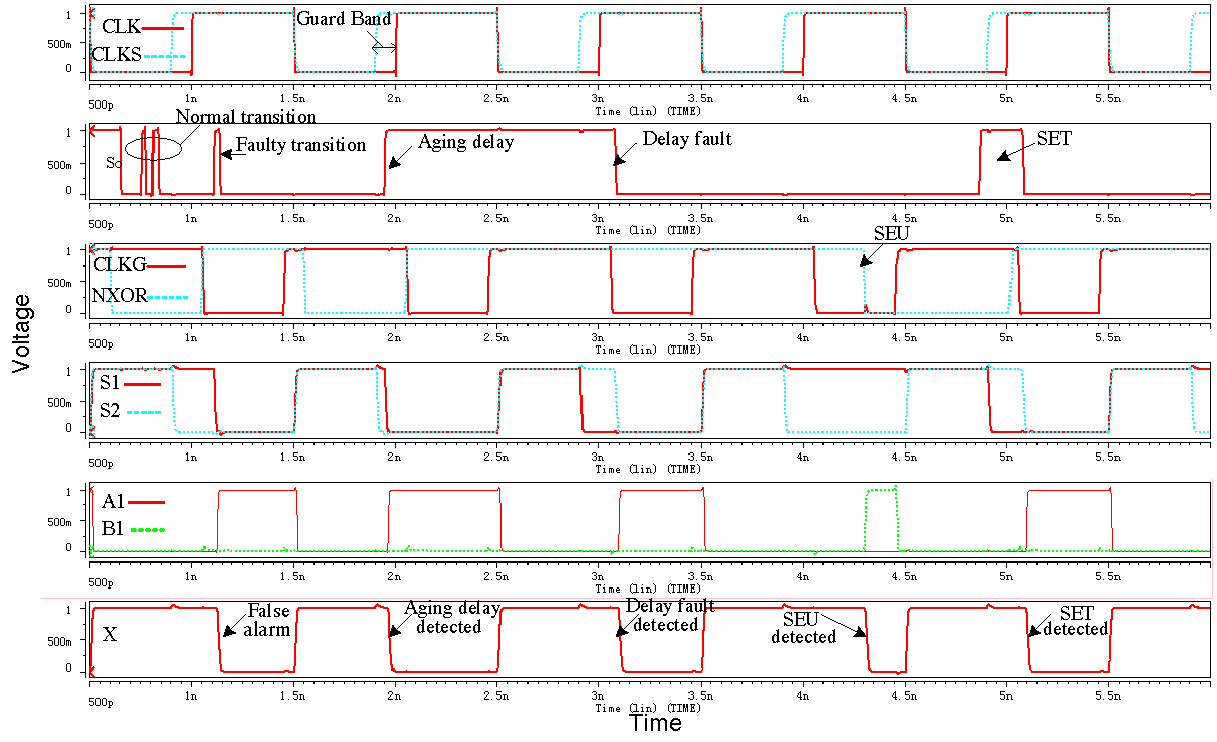
\includegraphics[width=0.99\textwidth, height=0.6\textwidth]{fig2-8}
\caption{Hspice simulated signal state transitions}\label{spice}
\end{figure}


\subsection{Experiment Result Analysis}
The experiments consist of two parts. The first is dedicated for evaluating a basic fault detection unit in terms of detailed timing verification, area overhead, power, and performance. The results are obtained by using the Hspice targeting the next-generation 32nm Predictive Technology Model \cite{PTM_06} for High-performance applications.  The second shows an application to a fully pipelined FPU, with emphasis on analysis of chip-level area and power overhead and comparisons with other solutions.

\begin{table}[t]
\begin{center}
  \setlength{\tabcolsep}{2mm}
\caption{Comparing Tradeoffs with other schemes}
\label{comparison1}
\begin{tabular}{@{}lccccc}
\toprule
 {\bf Overhead}     &  SEFF\cite{Mitra_C05}  &  LOWCOST\cite{lowcost_date07} &  ARSC\cite{agarwal2007circuit}  &  CWSPFF\cite{CWSP_DATE08}    &  SVFD \\
 \midrule  
Transistor          & 14     & 36       & 24     & 46       &  36   \\
Power               & 1.00      & $>$1.00        & $>$0.10$^\triangleleft$   &  N/A     &  1.16  \\
performance         & 0      & N/A      & $<$1\% & $<$1\%   &  $<$1\%\\
Clock               & 1      &  2       &  2     & 2        &  3    \\
\hline
  {\bf Applicability}     & Limited$^\diamond$ & Limited &  General & General & General \\
\bottomrule 
 \multicolumn{6}{l}{N/A:  Not applicable.}\\
\multicolumn{6}{l}{$\diamond$  The scheme needs support from a specific scannable flip-flop.}\\
\multicolumn{6}{l}{$\triangleleft$  ARSC uses a different metric of power overhead.} \\

\end{tabular}
\end{center}
\end{table}


\subsubsection{Evaluating SVFD Unit}
Figure \ref{spice} shows the detail timing of a SVFD unit in consecutive five cycles. The topmost shows the system clock CLK, the precharge-evaluation clock CLKS, with which the guard-band defined. The second shows the monitored signals $S_o$. The third illustrates the XOR-protection signal and corresponding gating clock. The fourth shows the state transitions of the two most important internal node S1 and S2. The fifth shows the signals A1---the output of the stability checker, and B1---the gated output of XOR protection unit. Both are feeded to the same compactor.The bottom most shows the detection result generated by the compactor.

During the first cycle (0---1ns), $S_o$ presents some normal transitions. In the first half of the second cycle (1---1.5ns), an unexpected glitch, which is supposed to simulate a benign SET fault, occurs; then in the guard band of the second cycle, an aging delay is simulated. A delay fault is simulated in the third cycle. In the fourth cycle, a SEU fault is simulated by pulling down the NXOR signal.

From the bottom figure, we can see that all the SV shown in the second and third waveforms are successfully detected, represented by LOW state of node X.

We zoom in the figure to extract some useful timing information (the zoomed figures are omitted due to space limitation): 1)the critical precharge time $\tau_0$ is about 40ps, while the available precharge time is about 400ps---one order of magnitude larger than $\tau_0$. Hence, the precharge time will not be a limitation when we manipulate the related timings. 2)The detection delay is just about 40ps which is merely 2 Fo4 delay in 32nm technology. 3)The maximum undetectable glitch width is about 18ps, which is even less than most soft error induce glitch width in 32nm technology, so the robustness of SET detection should not be in question.

Table \ref{comparison1} shows the tradeoff comparisons between SEFF \cite{Mitra_C05}, LOWCOST \cite{lowcost_date07}, ARSC \cite{agarwal2007circuit}, CSWPFF \cite{CWSP_DATE08}, and SVFD. we use the number of transistors as the area overhead metric, as many circuit-level studies adopted.

To conduct comparisons between variety schemes, a baseline latch and flip-flop design needs to be determined. Figure \ref{circuit}(e) and (f) show the adopted baseline design. The similar latch design is used by Intel as a standard datapath latch \cite{Latch_01}. The flip-flops is used in PowerPC603 processor \cite{Flipflop_94}. In addition, an XOR gate consumes at least 12 transistors when computing the number of transistors (eight transistors for the core XOR logic and another four for generating the inverter versions of input signals). For fairness, only the checker and its input generating logics are considered; the subcomponents that can be shared among checkers (i.e. output compactor, and output latches) are not taken into account though such amortization will make the area overhead of SVFD more attractive.

{\bf Area:} As Table \ref{comparison1} indicates, SEFF is most economic scheme in term of area overhead; however, this benefit has to be based on a dedicated scannable flip-flop design in which each functional flip-flop has a replica, called shadow flip-flop,  to support scan test. This heavy reliance on the specific scannable flip-flop, though greatly facilitate an area-efficient design, limits the applicability of SEFF, since not all designs use the same design-for-test techniques and implementation. LOWCOST can be regarded as a mutation of SEFF, but with a delay between the functional flip-flops and its' shadow counterpart. Thus, LOWCOST face the same issue of limited applicability. Clearly, if the shadow flip-flops are treated as overhead transistors, then the total transistors overhead must be much higher than that shown in Table \ref{comparison1}.

{\bf Power:} We use a relative power penalty $R_p$ to evaluate the power:

\begin{equation}
  R_p=\frac{\mbox{Power of a detection unit}}{\mbox{Power of a flip-flop}}.
\end{equation}

We compare the power of the detection unit against that of a standard flip-flop, respectively, with the same input signal and frequency. The input signal changes value every cycle. The Hspice results show that the stability checker is relatively power-hungry---16\% higher than the power of a flip-flop.  This is mainly because the checker is implemented with dynamic circuit style. The Compactor logic, however, is much power-saving---a 8-input compactor only consumes 40\% power of a flip-flop; this because when fault-free, all input signals fed to a compactor won't discharge it. The power of output latches even drop to only 10\% of a flip-flop because there no state transition happens to the latch during fault-free state, thus no dynamic power consumed.

As for other solutions,  SEFF's power is doubled ($R_p=1$), as \cite{Mitra_C05} shows, since a redundancy flip-flop is enabled. Similar modification is conducted in LOWCOST, and moreover an extra lath is employed; hence the power of LOWCOST must be slightly larger than that of SEFF ($R_p>1$).

Note that our checker seems much more power-hungry than ARSC. That is because the power overhead metric in \cite{agarwal2007circuit} is different with ours. In ARSC, the power overhead is calculated as the whole logic (include both the flip-flop and combinational logic) power increase. Because the combinational logic's power is relatively constant, so the actual sensor power consumption compared with a flip-flop should be much higher.

{\bf Performance:} The performance mainly depends on the flip-flops time overhead and the critical path delay. In SVFD, there is no modification to the flip-flops and the critical path is not changed as well. The only timing penalty results from several extra gate capacitances drived by the $S_i$ and $S_o$. Our experiment result shows this penalty is less than 1\% for a special combinational logic: 8-inverter chain.  In fact, the other SEFF, LOWCOST, ARSC, and CWSPFF face the same situation, but no one get hurt from it.

{\bf Clock:} We compare the number of clock (phase) used by these schemes. For example, SEFF dose not need any extra clock; LOWCOST, ARSC, CWSPFF, need one extra clock skewed with respect to the system clock. while SVFD needs two extra clocks: CLKS and CLKG. This is a negative attribute of SVFD since the extra clocks could potentially increase the complexity; as a tradeoff, however, the SVFD's detection capability is the most versatile over the other four schemes.

{\bf Applicability:} The SEFF and LOWCOST need the support from a particular type of scannable flip-flop, but the other three schemes do not suffer from this limit.

\subsubsection{Case Study---An application of SVFD}

We use a case study to demonstrate the main considerations when deploying SVFD, with emphasizing on area and power implications.

The pipelined FPU adopted by OpenSPARC T1 \cite{OpenSPARC_06} is used as our target circuit which implements the SPARC V9 floating-point instructions and supports all IEEE 754 floating-point data types. The FPU comprises three independent pipelines: Multiplier pipeline (MUL), Adder pipeline (ADD) and Divider pipeline (DIV). More design details can be found in \cite{OpenSPARC_06}.

The FPU was synthesized using Synopsys Design Compiler with UMC 0.18um technology, with performance as the synthesizing priority.

\vspace{0.3cm} \noindent{\bf Experimental Setup}

First, several timing parameters are determined. Specifically,
\begin{itemize}
  \item The cycle period $T$ is defined according to $t_{pd}$; given 10\% margin reserved,   $T={10}/{9}\times t_{pd}$. The critical path delay ($t_{pd}$) reported by PrimeTime is $1.7ns$, so $T=1.87$ns.

  \item The clock-to-q time $t_{cq}$ depends heavily on a specific flip-flop design and technology. Given 180nm technology for the design in Figure \ref{circuit}(f),  $t_{cq}$ is about 110 ps; Thus, we get $t_{cq} = 0.06T$.

  \item  Next, $t_{cd}$, $T_DS$, and $T_{GB}$ needs to be determined. We prefer minimize $t_{cd}$ since larger $t_{cd}$ implies more path compensation area needed to pay, while check whether $T_{DS}$ and $T_{GB}$ meets the common requirement, for example, $T_{DS}\approx0.5T$ and $T_{GB}>0.05T$ \cite{lowcost_date07} \cite{agarwal2007circuit}. From (\ref{eq82}), we figure out the minimal $t_{cd}$ is 0.79ns ($0.43T$), at which $T_{GB}=0.095T$, $T_{DS}=0.48T$. Then, we check out that $T_{GB}$ indeed meets the requirement: larger than $0.05T$ while less than timing margin ($0.1T$). $T_{DS}$, however, is slightly smaller than $0.5T$; considering such minor mismatch won't impose any substantial problem for delay fault and SET detection, we prefer to keep $T_{DS}=0.48$ while paying the minimal path compensation overhead.
\end{itemize}

Second, at register transfer level (RTL), we integrated parts of the SVFD infrastructure---the XOR-Protection, XOR-Trees, AND-Trees---into the target FPU. It is difficult to integrate corresponding stability checkers and compactors because these logic are highly custom dynamic logic at transistor-level; however, since we focus on overhead evaluation, so this difficulty can also be resolved in an "indirect" way. The area overhead imposed by these dynamic logic is estimated based on the data in Table \ref{comparison1}. The short-path compensation is realized by imposing a timing constraints when conducting RTL synthesis. After the compensation process, we conduct the post-simulation to verify pipelines functionality and timing.

Third, we use PrimePower (a gate-level power simulation and analysis tool provided by Synopsys for power evaluation. The modified FPU are exercised with random input operands for 100,000 cycle, at the same time, dump the according VCD (Value Change Dump) format data for power evaluation. The power of checkers and compactors are still evaluated with Hspice. We wrote a C++ program to convert the output of the XOR-Trees and AND-Trees (VCD format) into PWL voltage sources which are recognizable for Hspice version checker and compactor to conduct a transistor-level power evaluation. Then, the Hspice-reported power is scaled to fit PrimePower-reported power based on $R_p$, thereby obtaining the overall power consumption.

\begin{figure}
\centering 
\subfigure[Area overhead and associated overhead breakdown] {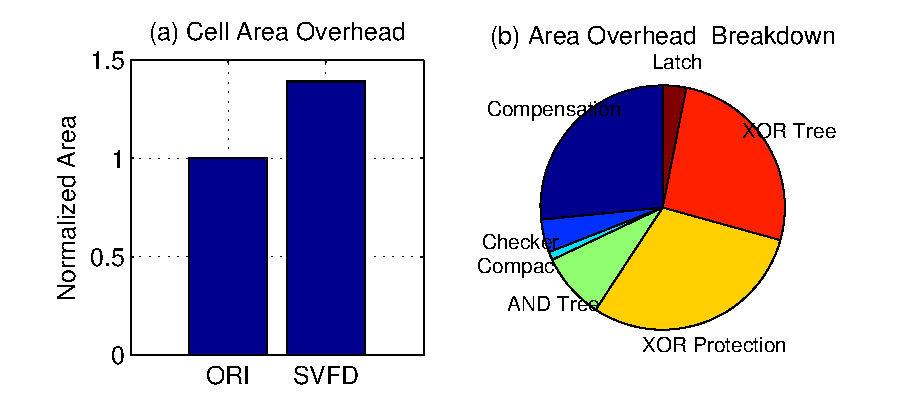
\includegraphics[width=0.6\textwidth]{fig2-9a}} 
\subfigure[Power overhead and associated overhead breakdown] {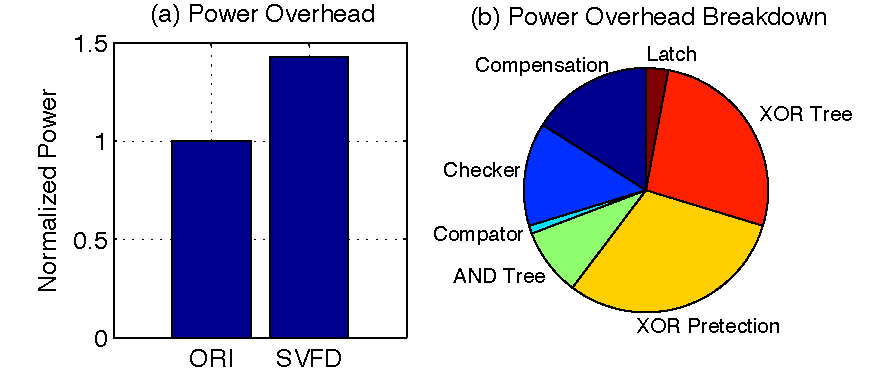
\includegraphics[width=0.6\textwidth]{fig2-9b}}
\caption{Area and power with configuration: $L_{xor}=3$, $L_{and}=3$, $BW=8$.} \label{area_power}
\end{figure}

\begin{figure}
\centering \subfigure[Implication of $L_{xor}$ and $L_{and}$ on area overhead]
{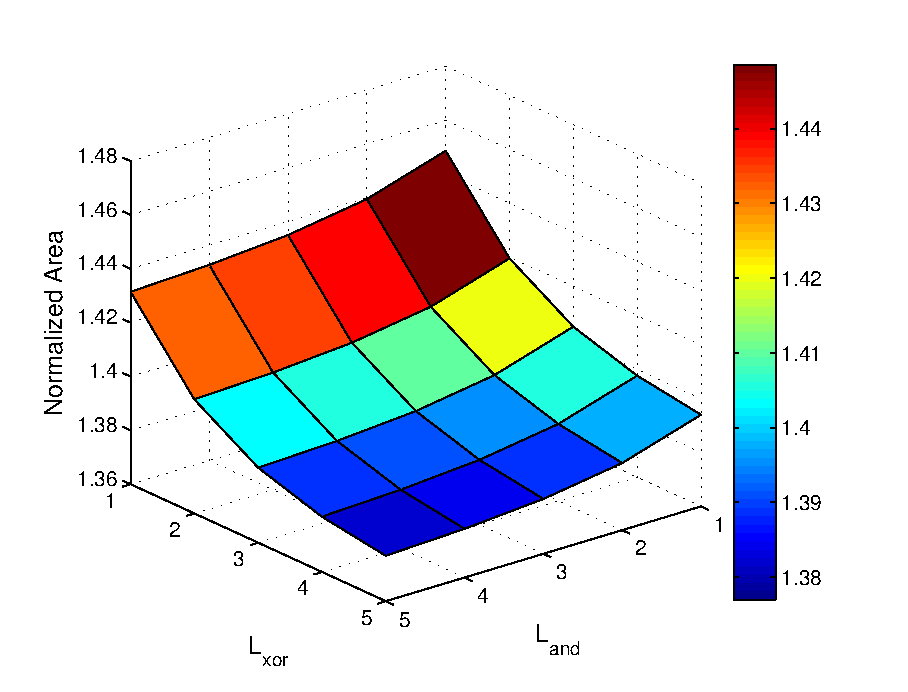
\includegraphics[width=0.48\textwidth]{fig2-10a}}  \subfigure[Implication of
$L_{xor}$ and $L_{and}$ on power overhead]
{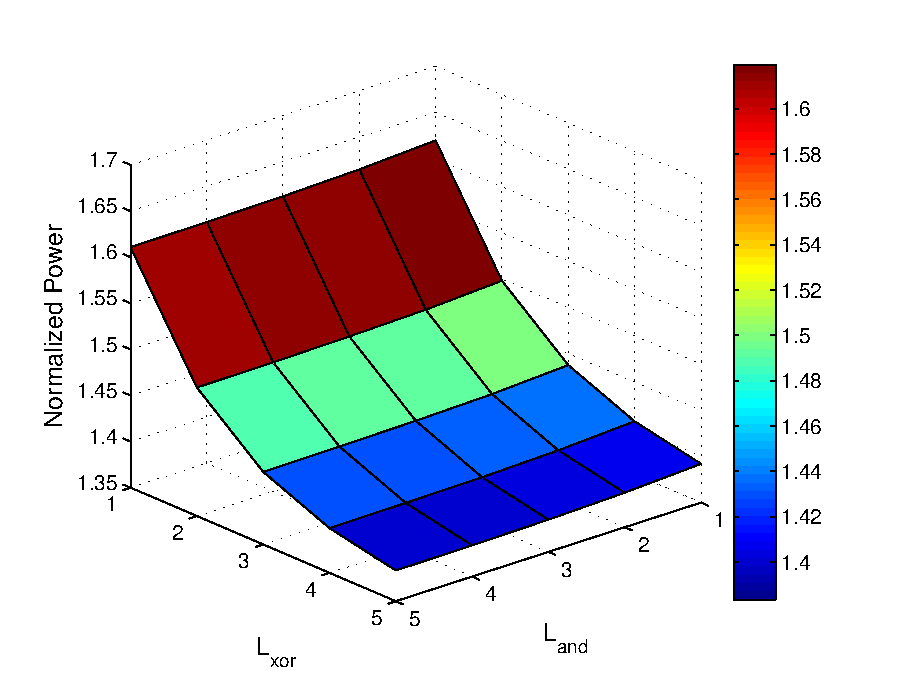
\includegraphics[width=0.48\textwidth]{fig2-10b}} \caption{Implication of
$L_{xor}$ and $L_{and}$ on area and power, $BW=8$.} \label{lxor_land}
\end{figure}

\vspace{0.3cm}\noindent{\bf Experimental Results}
The configurable parameters are 1) the level of XOR-Tree ($L_{xor}$), 2) the level of AND-Tree ($L_{and}$), and 3) the bandwidth of the compactor ($BW$). We first study the overhead at the tentative configuration: $L_{xor}=3$, $L_{and}=3$, $BW=8$, and then seek to optimize it. Figure \ref{area_power} shows the corresponding experimental results.

Figure \ref{area_power}(a) compares the SVFD's area, denoted by SVFD, against that of the original FPU, denoted by ORI. The total cell area overhead is about 40\%. This overhead comes from 1) compensating the short path to meet the $t_{cd}$ requirement, 2) the stability checkers and associated compactors  and latches, 3) the AND-Trees and XOR-Trees, and 4) the XOR-gates for XOR protection. Among these breakdowns of area overhead, “ompensation" and ”XOR Protection" are constant for a given target circuit because the former is determined by the minimal contamination delay and the later by the number of flip-flops; however, the other portions are configuration-specific. The corresponding power implication is shown in Figure \ref{area_power}(b). The overall power overhead is 43\%. In addition, two significant implications, which can guide to a more efficient configuration, can be drawn from these results:
\begin{enumerate}
  \item  The checker's area and power are unproportionate:  4\% area overhead   contributing to 14\% power penalty. Hence, reducing the number of checkers should   be an effective way to optimize the  overall power penalty.

  \item  Increasing the $BW$ of compactors has very marginal benefit to reducing the overall area and power since the area and power of the compactors and associated output latches together take only 4\% and 3\%, respectively.
\end{enumerate}

One way to reduce the number of checkers is to adopt the XOR-Trees with higher levels. The same strategy can be considered to optimize the overhead imposed by AND-Trees. Figure \ref{lxor_land} shows the overhead trends with different $L_{xor}$ and $L_{and}$ configurations.

The first perception gained from this figure is the power issue is much more crucial than the area issue: the worst-case power penalty can reach up to 1.62$\times$ while the area is only 1.45$\times$. In addition, the headroom for area optimization is limited comparing with that of power optimization. Hence, prioritizing the power optimization should be much effective for reaching an optimum design tradeoff. In SVFD scheme, power optimization actually does not conflict with area optimization.

Second, both the area and power trends are more sensitive to $L_{xor}$ than to $L_{and}$. In particular, as Figure \ref{lxor_land}(b) shows, the impact of $L_{and}$ to the power is almost negligible. Note that although increasing $L_{xor}$ and $L_{and}$ seems facilitate more area- and power-efficient deployment, we should keep the delay implication of the XOR-Tree and AND-Tree in mind. For the pipelined FPU implemented with 180nm technology, the $T$ is about 17 Fo4 ($\approx 1.9ns/110ps$). We suggest configuring the XOR-Tree with fours levels, and the AND-Tree with five levels. With this configuration, the following will compare SVFD with several recently proposed solutions from cell area and power aspects.

\begin{figure*}[!t]
\centering \subfigure[] {
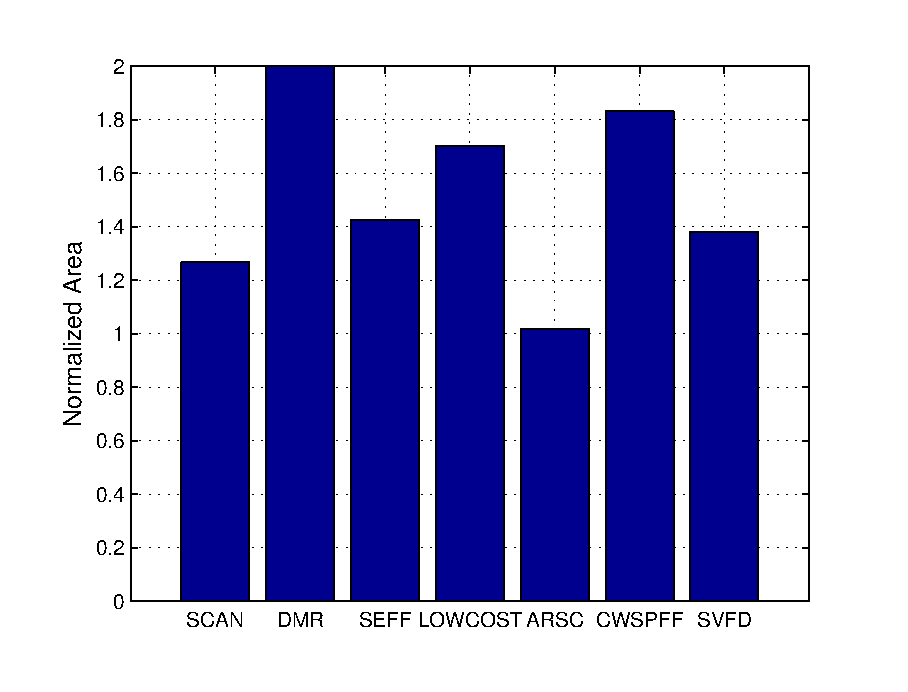
\includegraphics[width=0.47\textwidth]{fig2-11a}}\subfigure[] {
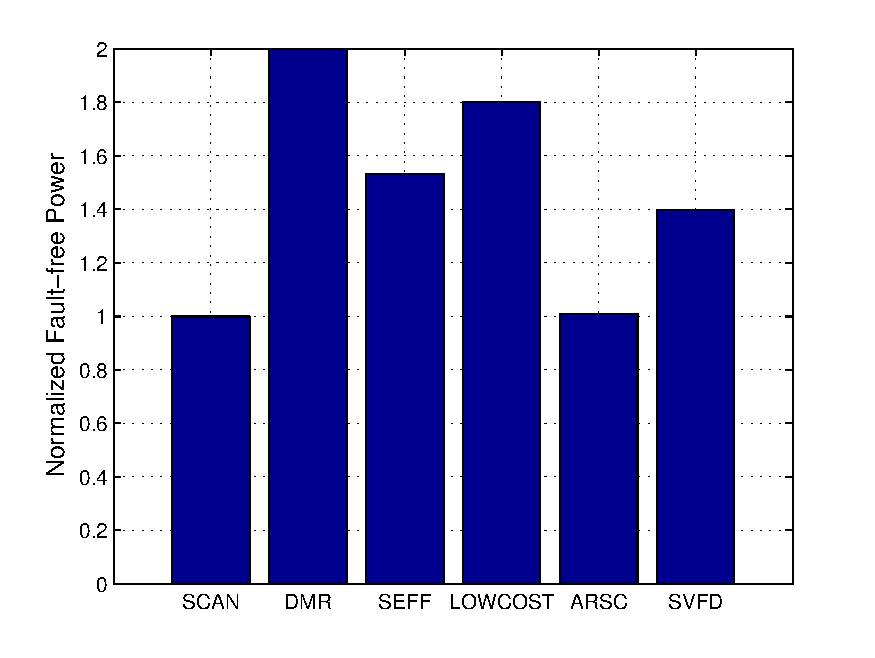
\includegraphics[width=0.47\textwidth]{fig2-11b}}
\caption{Comparison with other solutions in terms of cell area and power,
$L_{xor}=4$, $L_{and}=5$, $BW=8$.} \label{APcomparison}
\end{figure*}

\subsubsection{Comparison with other schemes}
Figure \ref{APcomparison} gives the comparison results. SCAN denotes the scannable version of the original pipeline. In SCAN, all pipeline flip-flops are substituted by a scannable flip-flops in \cite{Mitra_C05}. DMR represents the traditional dual-module-redundancy (we simply double the original area and power to show DMR's overhead implication. In fact, for any meaningful DMR, other synchronous overhead such as output comparison should be also imposed). SEFF is implemented by substituting the scannable flip-flops for a self-checking flip-flops \cite{Mitra_C05}. LOWCOST is substitute the scannable flip-flops with another modified flip-flops in which the clock of shadow flip-flop is skewed from that of the functional flip-flops; in addition, an output latch is also inserted \cite{lowcost_date07}. CWSPFF is also based on a slightly modified DFF and additional Equivalence checker, another shared logic whose overhead can be amortized by the other logics \cite{CWSP_DATE08}, but even we neglect the amortizable logics, we believe that this solution is also not overhead-economic, given the results indicated in Table \ref{comparison1}. ARSC is dedicated for only aging delay detection \cite{agarwal2007circuit}.

Figure \ref{APcomparison} (a) shows different total cell area required to deploy these solutions. In which, ARSC presets to be the most area-economic, this mainly because the ARSC logic only need to be deployed in the timing critical portions in terms of aging delay detection. The same reason, combined with the fact that the ARSC logic does not need to be always-on, makes the chip-level power overhead of ARSC negligible \cite{agarwal2007circuit}, as "ARSC" bar in Figure \ref{APcomparison} (b) shows.

We bar SCAN in Figure \ref{APcomparison} is not because it can facilitate some fault detection or recovery (actually it incapable for any fault detection), but it can be viewed as the foundation of SEFF and LOWCOST.

Figure \ref{APcomparison} shows that the overhead imposed by SVFD is very comparable with that of other schemes: the area overhead is 39\%, and the power penalty is 40\%---both are superior to that of SEFF scheme, while SEFF can only handle SEU faults. Given that SVFD can cope with SEUs, SETs, delay faults, aging delays; therefore, we conclude that the versatile SVFD is more promising.

Note that we omit the CWSPFF's power implication in Figure \ref{APcomparison} is because re-implement this scheme in our target pipeline is very labor-intensive and time-consuming. But considering the complexity of the CWSPFF logic and associated deployment, the power overhead should not superior than that of SEFF. In addition, compared with SVFD's versatile capability, CWSPFF can only handle SET faults.

%All of the above analysis is with respect to the ORI circuit. If we switch to with
%respect to the SCAN, the area overhead of SVFD will decrease and the power
%effectiveness of SVFD differs little.

\begin{table}[t]
\begin{center}
  \setlength{\tabcolsep}{2mm}
\caption{Comparison of detection capability }\label{comparison}
%\begin{tabular}{l|p{0.8cm}p{1.5cm}p{1cm}p{1.2cm}p{0.6cm}}
%\extrarowheight=1pt \tabcolsep=2pt
\begin{tabular}{@{}lccccc}
  \toprule
    &  SEFF\cite{Mitra_C05}  &  LOWCOST\cite{lowcost_date07} &  ARSC\cite{agarwal2007circuit}  &  CWSPFF\cite{CWSP_DATE08}    &  SVFD \\
\midrule
%\multicolumn{6}{c}{}\\

            SEU        &  Yes   & Yes    & No     & No     & Yes  \\
            SET        &  No    & Yes    & No     & No     & Yes  \\
            Aging delay&  No    & No     & Yes    & No     & Yes  \\
            Delay fault&  No    & Yes    &  No    & Yes    & Yes  \\
\bottomrule %\multicolumn{6}{l}{'---' :  Aging delay does not need any recovery routine.}\\
 %\multicolumn{6}{l}{'90\%':  fault coverage for SEU is $(1-0.095T/T)\approx 90\%$.}\\
\end{tabular}
\end{center}
\end{table}

\subsection{Discussion}
\subsubsection{On SVFD Application}
With the increasing impacts of soft errors and transistor aging under the relentless CMOS scaling, we believe SVFD will be increasingly promising. In part is because SVFD is far more area efficient than traditional DMR based schemes, in part for its versatile capability for fault detection. But SVFD does not suppose to totally take the place of existing approaches, especially ECC based schemes.  The following will discuss how to apply SVFD efficiently and why SVFD is a significant complement to existing schemes.

Modern processor includes two types of structures: logic-dominated structures such as execution units and memory-dominated structures such as register file, caches \cite{Revival_08}. Using  SVFD for logic-dominated structures, as the FPU in our experimental study, are cost-efficient. Since such type of structures usually are so non-regular that engineers mostly have to resort to coarse-grained DMR, thereby imposing more area and power overhead. Moreover, the SVFD can also indicate the aging process, which is an essential benefit that the traditional DMR can hardly achieve.

As for protecting the regular memory-dominated structures from in particular soft errors, ECC has been proven to be a highly cost-effective approach. SVFD can not beat ECC in terms power and area overhead, though SVFD can also detected soft errors in memory-dominated structures since soft errors induced perturbations can also results in stability violation in primary outputs. The prior research shows that, with extensive architectural hits such as register lifetime prediction \cite{Using_Register_Lifetime_dsn07}, selective placement \cite{Exploiting_selective_placement_taco08}, ECC-based approach commonly dictates about 30\% area overhead. This overhead is comparable with that of SVFD. While one ECC's benefit that SVFD does not possess is error correction---the commonly used ECC is able to correct single-bit fault and detect two-bit fault. Hence, we think ECC is still the preferred option for memory-dominated structures in a microprocessor.

But SVFD scheme offers aging prediction that ECC-based doesn't. The aging process of SRAM cells exhibits by increased read-out and write-into delay. The read delay is more critical than write delay because the read path usually serves as the critical path \cite{Mitigating_Parameter_Variation_micro07}. While for the SVFD sensors the degraded read operations behave the same with the degrade critical delay in logics, and hence can also be handled by a simplified SVFD sensors that are only for aging prediction---as Agarwal et al. proposed previously \cite{agarwal2007circuit}.

Hence, we conclude that SVFD is a cost-efficient application for protection logic-dominated structures; combined with ECC based approaches which can already handle soft errors, SVFD can also provided additional capability for aging prediction for memory-dominated structures.

\subsubsection{Variation and Aging Considerations}
Just as DMR cannot be free from false positive, SVFD face the same situation. The systematic variation hurts little to SVFD unit as well as other fault detection infrastructures because it statistically exhibits distinct spatial locality and correlation. If the SVFD suffers from the systematic variation, so does the host circuits in the same silicon spots. But random variation in some corner cases can invalid the SVFD unit. As shown in Figure \ref{circuit}, for example, if the leakage of M3 is overly large due to random variation, and at the same time the keeper for S1 happens to be too weak to compensate the escaped charge through M3, then a false alarm will be flagged. In other words, if S1's keeper does not happen to be that weak, the SVFD unit is highly probable to work. The same situation comes to M4. Therefore, on one hand, these keepers can help cancel out part of negative effects of random variation; on the other hand, we can properly size the transistors on the discharge paths to obtain more robustness against random process variation.

As the transistors in host circuits, the transistors in the SVFD unit also wear out over time. While the other hardware-based fault detection schemes such as LOWCOST and DMR suffer from the same situation. But the core logics, i.e. stability checker (Figure \ref{circuit}(b)) and compactor (Figure \ref{circuit}(c)) are relatively resistant to NBTI---one of the major aging mechanisms, because all of the PMOS transistors in the two logics are timing non-critical, while all the timing critical transistors are NMOS transistors which intrinsically are free from NBTI. Hence, we believe SVFD units have good chance to stand longer than the host circuits due to the better NBTI resilient characteristics.



\subsubsection{Distinguish Detection Results}
It is useful to  distinguish the aging delay caused detection positive from the rest of detection results,  because the detected aging delay rate is used as the input for some aging-aware designs.

SVFD implicitly apply a rule for distinguish the detected results. That is: If a stability violation is detected in Guard Band, then this violation is viewed as aging delay induced; the stability violation detected in other region is viewed as soft error or delay fault induced. Figure \ref{circuit}(d) is used to implement this rule. However, this might degrade the confidence level of detected aging delay rate since if a stability violation takes place within the Guard Band, SVFD can not determine whether this violation is caused by a soft error or an aging delay.

Fortunately, this confidence degradation incurred by this implementation is negligible. To quantitatively evaluate the miss rate, we define the miss as: a soft error induced stability violation is misjudged as an aging-fault stability violation.

Suppose that the raw soft error rate (SER), $R_{soft error}$, is uniformly distributed over time. The detectable SER is $\alpha R_{softerror}$, where the $\alpha$ is a constant ($0<\alpha<1$) related to the three masking effects \cite{Shivakumar_DSN02}. The aging fault rate is denoted as $R_{aging}$.

The misjudgment rate $R_{miss}$ can be expressed as
\begin{eqnarray}\nonumber
R_{miss}&=&1-\frac{R_{aging}}{R_{aging} + \alpha R_{soft error}\times\frac{T_{GB}}{T_{DS}+T_{GB}}}
\end{eqnarray}

Practically, the Guard Band should not be larger than the timing margin to avoid extra timing penalty. A typical timing margin is 10\%. Assume that $\alpha=0.5$, and $R_{soft error} =0.1\times R_{aging}$ (actually, after some detectable aging effects of devices begin emerging, the assumptions of $\alpha$ and raw SER are heavily conservative ), $T_{GB}/T_{DS}=0.2$ then $R_{miss}$ is not large than 1\%. Therefore, we can safely conclude that the imperfect distinguishing capability will not impose any substantial problem.

\section{On-Chip Path Delay Measurement}
In this paper, we present a novel on-chip path delay measurement architecture for efficiently detecting and debugging of delay faults in the fabricated integrated circuits. Several delay stages are employed in the proposed on-chip path delay measurement (OCDM) circuit, whose delay ranges are increased by a factor of two gradually from the last to the first delay stage. Thus, the proposed OCDM circuit can achieve a large delaymeasurement range with a small quantity of delay stages. A calibration circuit is incorporated into the proposed on-chip path delay measurement technique to calibrate the delay range of the delay stage under process variations. In addition, delay calibration for import lines is conducted to improve the precision of path delaymeasurement. Experimental results are presented to validate the proposed path delay measurement architecture.

\subsection{Path Delay Measurement and Fault Tolerance}
    With the scaling of semiconductor process technology, the performance of modern VLSI chips improves significantly. We have seen operating frequencies of integrated circuits reach multi-gigahertz, resulting in more rigorous timing requirements \cite{ITRS09} \cite{zeitzoff2002mosfet}. Timing related defects originated from manufacturing process-related problems, such as resistive opens and shorts, metal mouse bites, via voids, etc., will become more common \cite{hawkins2003view}. Consequently, delay faults caused by these physical defects, which prevent the circuit from meeting the timing requirements, are of growing concern in nanometer technologies \cite{krstic1998delay}. Moreover, it should be noted that the manufacturing process is becoming more difficult to be controlled with the increasing complexity of modern VLSI chips. Therefore, electrical parameters, such as saturation current, gate capacitance, threshold voltage, etc., may vary from one device to another. As a result, the delay of gates and timing-critical paths will have large variations and can hardly be predicted during the design stage due to the imprecision of verification models \cite{blaauw2008statistical} \cite{agarwal2003statistical}. Furthermore, the circuit timing would also be impacted by the application environment conditions such as temperature, supply voltage noise, etc. In order to improve the quality of shippable products, there is an urgent need to conduct effective delay testing for ascertaining the correct operation of chips at the rated frequency \cite{mak2004new} \cite{krstic1998delay}.

\subsubsection{Challenges for Path Delay Measurement}
Traditionally, at-speed delay testing is implemented to check the satisfiability of circuit timing by only considering whether the circuit under test (CUT) passes delay testing under the applied test vector pairs or not. However, under the process and environment variations, it requires to test the chip at different worst case timing scenarios to ensure the circuit’s timing correctness \cite{krstic2001delay} \cite{zhang2008multiple} \cite{fu2008robust}. For example, for a circuit path with a very small slack, even though it passes a test under the at-speed test clock frequency, it possibly fails another test that induces larger capacitive coupling or power supply noise.

The small delay defect (SDD), which introduces only a small extra delay over its normal value, may fail to be detected by at-speed delay testing due to the observability limitation for a large timing slack. However, the detection for SDDs is increasingly important to ensure the chip’s quality and reliability \cite{menon2009output} \cite{ahmed2006novel}. The first important reason is that a timing failure can be occurred in the circuit during functional application caused by the increment of small delay on paths with small timing slacks \cite{kruseman2004hazard}. The second important reason is that the SDDs hidden in the circuit may become one of the major reliability limiters \cite{nigh2000test} \cite{tayade2008small}. In addition to the imperative requirement for SDD detection, it is well known that in order to improve the yield and reduce the time-to-market of chips, design-related failures and performance limiters need to be identified and rectified as early as possible during first silicon debug \cite{balachandran2002facilitating}. However, it is very expensive to use external high-speed automatic test equipment (ATE) for post-silicon debug of modern high-performance chips. Moreover, the frequency of test clock generated by external ATE would be affected by factors such as parasitic capacitance, resistance of probe and tester skew, etc. \cite{sunter1998bist}. In addition, for a complex SoC, the internal circuit modules are limited to be accessed by the external ATE to conduct silicon debug.

The on-chip path delay measurement techniques have been gained many attentions for researchers in recent years, for it can provide a cost-effective alternative way to perform delay defect detection and silicon debug in modern VLSI chips. Rather than testing the chip with all possible worst-case test vectors and process corners, it is better to measure the delays of paths and to check if the slacks are large enough to tolerate all the possible delay variations. Therefore, high complexity for finding the worst case test vectors considering different sources of variations can be avoided and high test confidence can be obtained. Moreover, by on-chip measuring the delays of selected paths in the actual silicon, precise path timing information can then be obtained for circuit under actual operating conditions. As a result, whether there are SDDs on a path can be analyzed based on the measured path delay. Further, the amount of timing violations in the failing paths can be obtained under certain environment conditions \cite{datta2004delay} \cite{ datta2006scheme}. Valuable information, which points the performance limiter and source to circuit failure, can hence be obtained by the on-chip path delay measurement technique with a much higher confidence.

\subsubsection{Prior Path Delay Measurements}
Several on-chip architectures have already been proposed for delay testing and silicon debug in literatures. Ghosh et al. \cite{ghosh2006novel} presented a built-in delay-sensing circuit to improve the delay fault coverage of the CUT. The delay of the path under test is converted to a certain voltage height by using a saw-tooth waveform generated from the reference clock signal. By comparing the converted voltage with the reference voltage, delay fault of the target path can then be detected. The same technique is also used in \cite{raychowdhury2005novel} for speed binning of the high performance chips based on the delay measurement results for circuit’s critical paths. Hsiao et al. \cite{tayade2008chip} proposed a built-in parametric measurement circuit for time-interval measurement based on the dual-slop technique. The capacitor is first charged by the input voltage with a high slope, and then the capacitor is discharged with a known lower slope. Therefore, the time-interval can be derived from the discharging time based on the proportional relationship between the discharging time and input voltage. Wang et al. \cite{wang2008path} proposed a ring oscillator based scheme for path delay measurement. By configuring the path under measurement (PUM) and the returning loop into a ring oscillator, delay of the target path can be translated into oscillation period. Tayade et al. \cite{tayade2008chip} utilize a programmable capture generator to obtain a fast capture signal to conduct faster-than-at-speed testing. Small delay defects can then be efficiently detected by this approach. Moreover, delays of the selected paths in circuit can also be measured by sweeping the capture clock frequency. Datta et al. \cite{datta2006scheme} proposed an on-chip timing characterization scheme based on the skewed inverter delay line. First a pulse is generated by the triggered transitions of the start and end points of the PUM using the test vector, and then the width of pulse is recorded into the latching circuits by using pulse shaping technique. Datta et al. \cite{datta2004chip} proposed a modified vernier delay line (VDL) technique for path delay measurement. By using a balanced delay line, high-resolution capability for delay measurement can be provided. Based on the same principle of VDL technique, the delay scan chain is proposed in \cite{datta2004delay} to reuse the existing scan chain for path delay measurement. Tsai et al. \cite{tsai2008all} proposed a built-in delay measurement circuit consisting of coarse and fine blocks, which is an extension of the modified VDL technique. However, the above VDL based techniques require lots of delay stages to achieve a large measurement range \cite{pei2009low}. Moreover, the delays of the import lines, which connect the chosen PUM into the path delay measurement unit, are not considered, thereby posing a significant influence on the precision of path delay measurement.

\subsection{Path Delay Measurement Circuits}
In this section, we present the design of OCDM for path delay testing and silicon debug. As mentioned above, the previous VDL based delay measurement techniques need lots of stages to achieve a large delay measurement range under the pre-determined delay measurement resolution. Consequently, the goal of the proposed OCDM circuit is to reduce the number of delay stages in the VDL, thus to achieve a significantly less hardware overhead as well as less delay measurement time.

\subsubsection{Basic Structure and Operation}
The basic structure of the proposed OCDM circuit is shown in Figure \ref{fig:OCDM-fig1}, which can convert the path delay of the PUM into a series of digital values that can be stored in the flip-flops of the VDL chain. Each delay stage consisted in the VDL chain is constructed by a positive edge triggered D-type flip-flop, four multiplexes, and several buffers. In the proposed OCDM circuit, we assumed that the input $x$ is fed by the output of the PUM, while the input $y$ is fed by the input of the PUM. So $y$ always switches earlier than $x$ does during the delaymeasurement period. In order to explain the operation of the OCDM circuit, let’s consider the case that both the input and output signals of the PUM are rising transitions.

\begin{figure}[t]
\centering
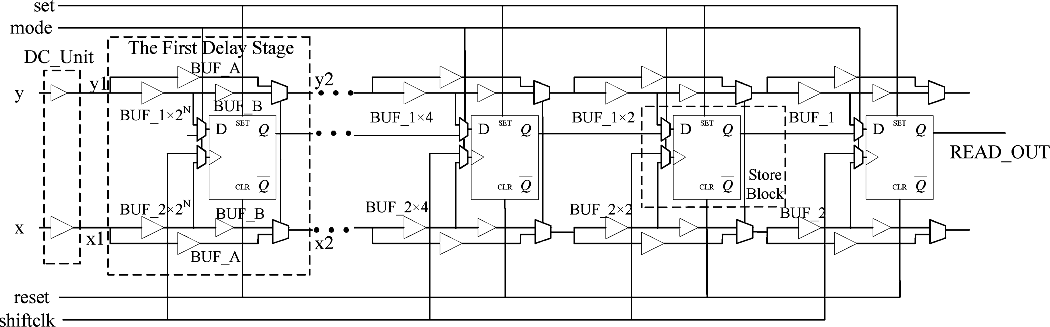
\includegraphics[width=0.95\textwidth]{OCDM-fig1}
   \caption{Proposed On-Chip Delay Measurement Circuit}
    \label{fig:OCDM-fig1}
\end{figure}


The upper delay unit (UDU) refers to the buffer chain that starts at the input of the delay stage at which the transition signal is propagated from node $y$, and ends at the input of the multiplexer whose output is connected to the data input of the flip-flop in each delay stage of the OCDM circuit. The lower delay unit (LDU) is similar to UDU, except that it starts at the input of the delay stage at which the transition signal is propagated from node $x$, and ends at the input of another multiplexer whose output is connected to the clock input of the flip-flop in each delay stage.

The delay range is defined as the delay difference between the two delay units in each delay stage of the OCDM circuit. For example, in the last stage of the OCDM circuit, the delay of UDU (named BUF\_1), $D_{buf\_1}$, is designed larger than that of LDU (named BUF\_2), $D_{buf\_2}$. Thus, the delay range of the last stage, $R_{last}$, is the delay difference between $D_{buf\_1}$ and $D_{buf\_2}$, i.e.,

\begin{equation} \label{eq:rlast}
    R_{last} = D_{buf\_1} - D_{buf\_2}.
\end{equation}

From the last stage to the first stage of the OCDM circuit, the delay range of each stage is increased by a factor of two. The DC\_Unit cell, as shown in Figure \ref{fig:OCDM-fig1}, is used for delay compensation, and will be explained in detail later. Two rising input transitions from the PUM pass through the DC\_Unit firstly, and then go into the inputs of the first delay stage of the OCDM circuit, respectively.

Let us explain the function of each delay stage by considering the operation of the first delay stage for the sake of clarity for illustration without loss of generality. Suppose the input and output signals of the upper delay chain in the first delay stage are $y1$ and $y2$, respectively, accordingly, $x1$ and $x2$ are assumed for the lower delay chain. All flip-flops of the OCDM circuit are initialized to logic ZERO values by asserting the reset signal. The delay measurementmode is activated by asserting the mode signal. As $x1$ and $y1$ signals propagate through their respective delay units, the time difference between the two signals will be reduced. As shown in Figure \ref{fig:OCDM-fig2}(a), assuming that $x1$ signal lags the $y1$ signal by enough time (i.e., $y1$ switches much earlier), and hence a logic-high value will be hold in the flip-flop. As a result, $y2$ will be the signal that passes through the UDU and the buffer BUF\_B in the upper delay chain from $y1$, while $x2$ will be the signal that passes through the LDU and the buffer BUF\_B in the lower delay chain from $x1$. The delay of BUF\_B is large enough to ensure that a stable logic high value can be stored in the flip-flop before the two transition signals arrive at the inputs of the multiplexers whose outputs are connected to the inputs of the next delay stage. Clearly, the time difference between $x2$ and $y2$ is reduced by an amount which equals the delay range of this delay stage.
\begin{figure}[t]
\centering
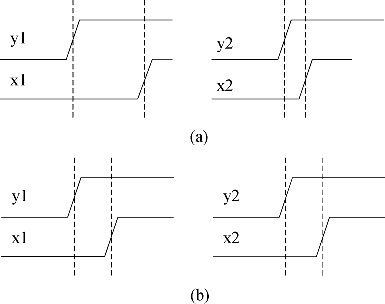
\includegraphics[width=0.45\textwidth]{OCDM-fig2}
    \caption{Relation between time difference of two input signals($x1$, $y1$) and that of two output signals ($x2$, $y2$) in the first delay stage. (a) Logic ONE in the flip-flop. (b) Logic ZERO in the flip-flop.}
    \label{fig:OCDM-fig2}
\end{figure}


The buffer named BUF\_A in each delay stage has a delay value that is larger than the cumulative delay of the path that contains LDU and BUF\_B of the same delay stage. Likewise, if the time difference of $y1$ and $x1$ is smaller than the delay range, the flip-flop will hold a logic ZERO value. Therefore, the signals propagating through BUF\_A are then selected by the multiplexers. As a result, the time difference between $y2$ and $x2$ will be equal to that of $y1$ and $x1$, as shown in Figure \ref{fig:OCDM-fig2}(b).

Consequently, the principle of the OCDM circuit is that if the time difference between the two inputs of each delay stage is lager than the delay range of the same stage, a logic ONE value will be stored in the flip-flop of the delay stage. The time difference between the two output signals will be updated by simply subtracting the delay range from that between the input signals of the delay stage. Otherwise, the flip-flop of the delay stage will hold a logic ZERO value, and the time difference between the output signals will keep the same as that between the input signals of the delay stage.


Note that there exists a setup time in the store block of each delay stage as shown in Figure \ref{fig:OCDM-fig2}, which consists of a D flip-flop and two multiplexers. If the time difference between the two inputs of the store block is smaller than the setup time (about 33ps in the experiment of this paper), an error logic value may be hold in the flip-flop. Therefore, in order to provide better delay measurement precision, the DC\_Unit cell constructed by two buffer lines is proposed for delay compensation, which means that the upper and lower delay units of DC\_Unit are designed such that the delay difference between them is approximately equal to the setup time. Meanwhile, if half of the delay range in the last delay stage is also compensated in the delay difference of the upper and lower delay units of DC\_Unit cell, the OCDM circuit can improve the delay measurement resolution by 50\%. The values stored in the delay line can be shifted out serially using the clock signal shiftclk in the shift mode by de-asserting the mode signal. The delay of the PUM can then be obtained.

\subsection{Delay Range Calibration}
The delay range of each delay stage in the OCDM circuit would be varied due to the prominent process variations. It is thus necessary to calibrate the delay ranges to assure the precision of path delay measurement result before using the OCDM circuit \cite{blaauw2008statistical} \cite{agarwal2003statistical} \cite{tsai2008all} \cite{datta2006scheme}. Figure \ref{fig:OCDM-fig3} shows the basic structure of the calibration circuit \cite{tsai2008all} \cite{datta2006scheme}, which can be embedded into the OCDM circuit for delay range calibration. The outputs of the calibration circuit, denoted as $y$ and $x$, are directly connected to the inputs with the same notations of the OCDM circuit, respectively.

\begin{figure}[t]
\centering
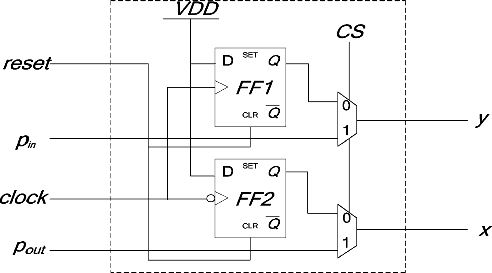
\includegraphics[width=0.45\textwidth]{OCDM-fig3}
   \caption{Calibration Circuit}
    \label{fig:OCDM-fig3}
\end{figure}


Two inputs of the calibration circuit, denoted as $P_{in}$ and $P_{out}$, are fed by the input and output of the PUM, respectively. Clearly, when the CS signal is set to 1, the generated transitions at the $P_{in}$ and $P_{out}$ can be sent into the OCDM circuit for delay measurement. When the CS signal is set to 0, the delay range calibration process is conducted.

The simplified timing waveform for the delay range calibration is shown in Figure \ref{fig:OCDM-fig4}. The FF1 and FF2 are rising and falling edge triggered flip-flops respectively. First, the flip-flops of FF1 and FF2 are initiated with logic ZERO by the reset signal. Then, logic ONE will be loaded into the FF1 and FF2 by the rising and falling edges of the clock signal respectively. Clearly, the time difference between the generated rising transitions at $y$ and $x$ is equal to the width of the positive half cycle of the clock signal. The time period of the clock signal can be programmed deterministically with high resolution using the on-chip clock generator from \cite{kaeriyama20071}.

\begin{figure}[t]
\centering
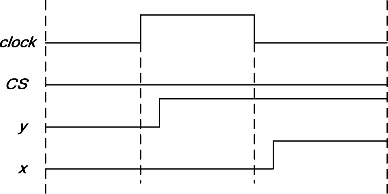
\includegraphics[width=0.45\textwidth]{OCDM-fig4}
   \caption{Simplified timing waveform for calibration circuit.}
    \label{fig:OCDM-fig4}
\end{figure}


Assuming the number of delay stages in the OCDM circuit is $m$. The following presents the calculation method for obtaining the delay range of each delay stage, which is described by Equation \ref{eq:eq-array}:
\begin{equation} \label{eq:eq-array}
    \begin{cases}
        a_{11}x_{1} + a_{12}x_{2} + ... +a_{1m}x_{m}=b_{1} \\
        a_{21}x_{1} + a_{22}x_{2} + ... +a_{2m}x_{m}=b_{2} \\
        ... \\
        a_{m1}x_{1} + a_{m2}x_{2} + ... +a_{mm}x_{m}=b_{m} \\
    \end{cases}
\end{equation}

Let

\begin{equation}
    A=
    \left[
    \begin{array}
        {cccc}
        a_{11} & a_{12} & ... & a_{1m}\\
        a_{21} & a_{22} & ... & a_{2m}\\
        ... & & & \\
        a_{m1} & a_{m2} & ... & a_{mm}\\
    \end{array}
    \right]
\end{equation}

\begin{equation}
    X=
    \left[
    \begin{array}
        {c}
        x_{1} \\
        x_{2} \\
        ... \\
        x_{m} \\
    \end{array}
    \right]
\end{equation}

\begin{equation}
    B=
    \left[
    \begin{array}
        {c}
        b_{1} \\
        b_{2} \\
        ... \\
        b_{m} \\
    \end{array}
    \right]
\end{equation}


The we can get Equation \ref{eq:array-abbr}.
\begin{equation} \label{eq:array-abbr}
    AX=B
\end{equation}

where $x_{j} \in (1 \leq j \leq m)$ in vector X represents the delay range of the $j$th delay stage to be calculated, $b_{i} \in (1 \leq i \leq m)$ in vector $B$ represents the width of the positive half cycle of signal clock for the $i$th calibration process, $a_{ij}$ in  matrix $A$ represents the measured value (0 or 1) for the $j$th delay stage during the $i$th calibration. Clearly, by selecting appropriate values for vector $B$ in each calibration process, it is easy to conclude the delay range for each stage by solving Equation \ref{eq:array-abbr}.

For example, assuming there are four delay stages in the OCDM circuit and we know their nominal designed delay ranges. After we choose 70, 55, 40, and 25 for $b_{i}$ in four calibration processes respectively, the obtained values for matrix A is listed as follows:

\begin{equation}
    A=\left[
        \begin{array}
            {cccc}
            1 & 1 & 1 & 0 \\
            1 & 0 & 1 & 1 \\
            1 & 0 & 0 & 0 \\
            0 & 1 & 0 & 1 \\
        \end{array}
        \right]
\end{equation}

Hence, after solving Equation \ref{eq:array-abbr}, the delay ranges are found to be 40, 20, 10, and 5 from the first to the last stage, respectively.

Note that the value of $b_{i}$ in the vector $B$, which is the width of the positive half cycle of the clock signal, may not be exactly equal to the expected value because of the clock jitter, and hence may induce error delay ranges for the delay stages. However, this can be compensated by multiple calibrations under each value because the clock jitter is a zero-mean random variable \cite{jan2003digital}. 

For example, if for the second calibration process is set to 55, the values in the second row of matrix $A$ are then expected to be equal to (1, 0, 1, 1) respectively. This can be represented by Equation \ref{eq:sum}.

\begin{equation} \label{eq:sum}
    55 = x_{1} + x_{3} + x_{4}
\end{equation}

However, if the width of the positive half cycle of the clock signal is varied from the expected value and is 50 or 60 due to the clock jitter, then the second row of matrix will get (1, 0, 1, 0) or (1, 1, 0, 0), respectively. Hence, the second row of matrix is replaced to Equation \ref{eq:sum13} or Equation \ref{eq:sum12} as follows:

\begin{equation} \label{eq:sum13}
    55 = x_{1} + x_{3}
\end{equation}

\begin{equation} \label{eq:sum12}
    55 = x_{1} + x_{2}
\end{equation}


Therefore, error values would be calculated for the delay ranges of the delay stages by using Equation \ref{eq:sum13} or Equation \ref{eq:sum12}. However, since the clock jitter is a zero-mean random variable \cite{jan2003digital}, we can calibrate the delay ranges using the same expected $b_{i}$ value for multiple calibration times. Though neither Equation \ref{eq:sum13} nor Equation \ref{eq:sum12} can be used to obtain the delay ranges correctly, the sum of the expressions obtained by multiple calibrations would be qualified. For example, by summing up Equation \ref{eq:sum}, Equation \ref{eq:sum13}, and Equation \ref{eq:sum12}, we can conclude Equation \ref{eq:sumall}.

\begin{equation} \label{eq:sumall}
    165=3x_{1} + x_{2} + 2x_{3} + x_{4}
\end{equation}

As mentioned above, the delay ranges are 40, 20, 10, and 5 from the first to the last stage, respectively, and can verify the correction of Equation \ref{eq:sumall}. Hence, the delay range of each delay stage can be calibrated by the process mentioned above. The calibration errors caused by the clock tuning resolution and measurement resolution are small and can be ignored. They can also be compensated by multiple calibrations using multiple number of $b_{i}$ values.

\subsection{Path Delay Measurement Architecture}
The architecture of the proposed path delay measurement scheme using the OCDM circuit is shown in Figure \ref{fig:OCDM-fig5}. The paths selected for delay measurement can be timing-critical pathswhose delays exceed the specified timing threshold under static timing analysis (STA) or statistical STA \cite{he2010fast} \cite{fu2010testable}. Based on the selected timing-critical paths, the method proposed in \cite{lesser1980experimental} provides an effective way to further find an optimal path set for measurement, while the delays of all the selected timing-critical paths can be obtained either by direct measurement or by calculation from the measured delays. In this paper, we mainly focus on the design of the path delay measurement architecture. Two M-to-1 multiplexers are included aiming to select a particular path into the OCDM circuit for delay measurement.

\begin{figure}[t]
\centering
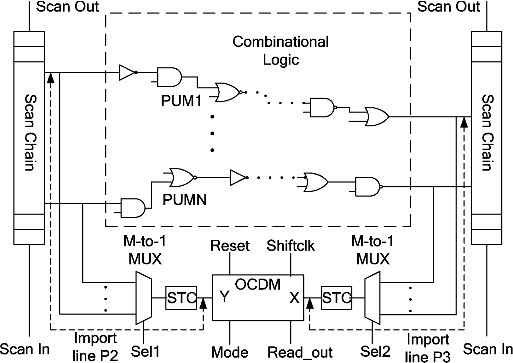
\includegraphics[width=0.56\textwidth]{OCDM-fig5}
   \caption{Path delay measurement architecture.}
    \label{fig:OCDM-fig5}
\end{figure}


\subsubsection{Signal Transition Conversion (STC)}
As mentioned in the previous section, the OCDM circuit works well only when the input and output of the PUM are rising transitions. However, there are other three additional cases possibly to activate the worst case delay of a circuit path, such as a path in which the input is a rising transition and the output is a falling transition. It is thus better to transfer the output signal into the signal with rising transition for facilitating path delay measurement regardless of the transition direction of the original signal.

The STC block shown in Figure \ref{fig:OCDM-fig5} is used to handle this problem. Therefore, rising transitions which are derived from the start and end points of PUM can be fed into the inputs and of the OCDM circuit, respectively. Figure \ref{fig:OCDM-fig6} shows the basic structure of the STC block, which is previously designed for signal stability violation detection in \cite{favalli1996sensing} \cite{agarwal2007circuit} \cite{SVFD_09}. The simplified timing waveform for the STC block is shown in Figure \ref{fig:OCDM-fig7}(a) and (b), respectively. When the pre-charge signal is low, denoted as the pre-charge period, both the nodes and are charged up to logic high values. Hence the OUT signal keeps a logic low value.

\begin{figure}[t]
\centering
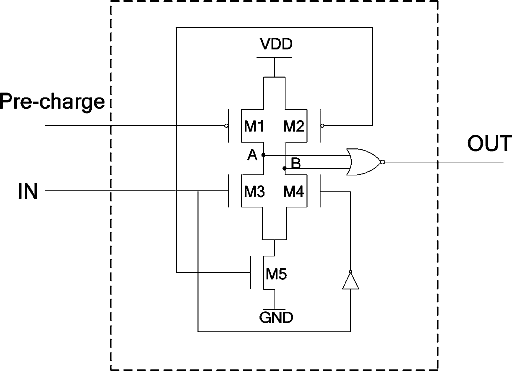
\includegraphics[width=0.46\textwidth]{OCDM-fig6}
    \caption{Signal Transition Conversion (STC).}
    \label{fig:OCDM-fig6}
\end{figure}

\begin{figure}[t]
\centering
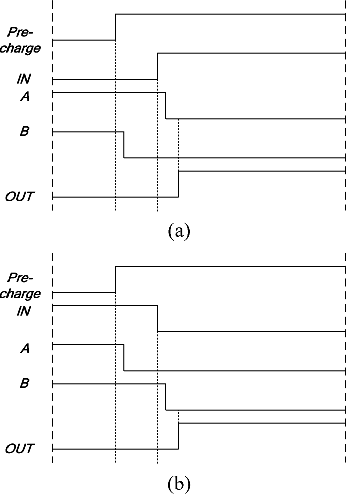
\includegraphics[width=0.48\textwidth]{OCDM-fig7}
    \caption{Simplified timing waveform for signal transition converter. (a) A rising transition at IN. (b) A failing transition at IN.}
    \label{fig:OCDM-fig7}
\end{figure}


Clearly, as shown in Figure \ref{fig:OCDM-fig7}(a), if a rising transition is generated at the IN signal when the pre-charge signal is high, both the node $A$ and node $B$ are discharged to logic low values after the arrival of the rising transition of IN. Therefore, a rising transition is generated at the OUT signal. Likewise, as shown in Figure \ref{fig:OCDM-fig7}(b), a rising transition would also be generated at the OUT signal after the arrival of a falling transition of the IN signal. Hence, by using the STC block, the input signal with arbitrary transition direction can be converted into a rising transition signal for facilitating path delay measurement.

\subsubsection{Delay Measurement}
The proposed on-chip delay measurement flow can be divided into eight steps as follows:
\begin{enumerate}[{1)}]
    \item Select the paths for delay measurement;
    \item For each PUM, the input and output transition signals of the PUM can be fed into the OCDM circuit for delay measurement by using the two M-to-1 multiplexes;
    \item The first vector of the test vector pair for the PUM is applied to initialize the internal logic of the circuit to a stable state; 
    \item All flip-flops of the OCDM circuit are initialized to logic ZERO values by asserting the reset signal; 
    \item The delay measurement mode is activated by asserting the mode signal; 
    \item The second vector of the test vector pair is applied to the circuit, and hence a transition signal can be launched at the input of the PUM, and propagated to the output of the PUM; consequently, the delay difference of the two transition signals is measured by the OCDM and recorded into the delay line; 
    \item After the completion of delaymeasurement, the OCDM circuit is configured into shift mode by de-asserting the mode signal. Therefore, the values stored in the delay line can be shifted out serially using clock signal shiftclk. Consequently, the path delay of the PUM can be calculated from the values read out.
\end{enumerate}

All paths can be selected for delay measurement by repeating the above steps 2–7.

After the values stored in the delay line have been read out, the delay of the PUM can then be obtained. Suppose the total number of delay stages in the OCDM circuit is $N$, the delay measurement resolution of the OCMD circuit is $M_{res}$, which is half of the delay range in the last delay stage $D_{las}$, and the values stored in the flip-flop from the first delay stage to the last delay stage of the OCDM circuit are $D_{N}$ to $D_{1}$, respectively. Then the path delay can be calculated as follows:


Delay of Measurement = $\sum_{i=1}^{i=N}D_{i} \times 2^{i-1}\times D_{las}$

The range of the path delay is then given as
$\sum_{i=1}^{i=N}D_{i} \times 2^{i-1} \times D_{las} - M_{res} <$ Path Delay $\sum_{i=1}^{i=N} \times D_{i} \times 2^{i-1} \times D_{las} + M_{res}$

The calculated path delay value of the PUM is then compared with the expected delay value for timing validation and silicon debug. The maximum delay measurement range of the OCDM circuit can also be obtained as follows.

Maximum measurement range = $\sum_{i=1}^{i=N} \times 2^{i-1} \times D_{las}$

\subsubsection{Delay Calibration for Import Lines}
In order to obtain the delay of the PUM with high precision, the delay of import lines $P_{2}$ and $P_{3}$ for feeding the start and end transitions of the PUM into the OCDM circuit, as shown in the Figure \ref{fig:OCDM-fig5}, should be taken into account. The reason is that it is difficult to mutually cancel the delays of the import lines $P_{2}$ and $P_{3}$ during physical design. Even though a careful custom layout can be conducted to balance the import lines $P_{2}$ and $P_{3}$ serving for one PUM, it can be hardly to satisfy this restriction for the import lines for all the PUMs. Moreover, the delays of import lines $P_{2}$ and $P_{3}$ would also be affected by the process variations and hence would bring a precision loss of the delay measurement. In order to address this problem, a 2-to-1 multiplexer is added for the flip-flop which is the end point of the PUM.


Figure \ref{fig:OCDM-fig8} redraws the architecture of the path delay measurement scheme shown in the Figure \ref{fig:OCDM-fig5}, which includes a 2-to-1 multiplexer with data inputs, respectively, connected to the data-input and data-output of the flip-flop at the end point of the PUM to calibrate the delay difference of import lines. 
\begin{figure}[t]
\centering
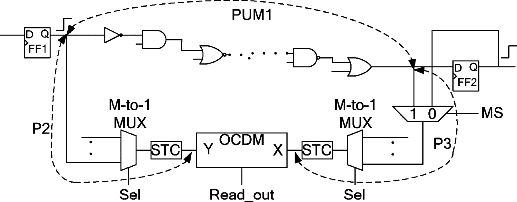
\includegraphics[width=0.6\textwidth]{OCDM-fig8}
    \caption{Delay calibration for improt lines}
    \label{fig:OCDM-fig8}
\end{figure}


When the MS signal is set to 1, the path delay measurement architecture is configured into the delay measurement mode. Hence the input and output of PUM1 are selected into the OCDM for delay measurement. The delay measurement result of PUM1 without considering the delay difference of import lines and can be represented as follows: 

Delay measurement result $= D_{1} + D_{3} - D_{2}$

where the $D_{1}$, $D_{2}$, and $D_{3}$ represent the delays of $PUM1$, $P_{2}$, and $P_{3}$, respectively. However, in order to obtain the delay of the PUM with high precision, the delay value of $D_{3} - D_{2}$ should be obtained firstly. The delay of $P_{3}$ is typically larger than that of $P_{2}$ for the insertion of a multiplexer. When the MS signal is set to 0, the import line’s delay difference calibration mode is configured.

For the first case, if the PUM is started at one flip-flop and ended at another flip-flop, then either rising or falling transition can be simultaneously generated at the outputs of the start and the end flip-flops by shifting the test vector with specific values into them. Hence the transitions generated at the outputs of the start and end flip-flops will pass through and into the OCDM circuit, respectively. Therefore, the delay difference of $P_{3}$ and $P_{2}$ can be obtained by the OCDM circuit under the import line’s delay difference calibration mode. For the second case, if the PUM is started and ended at the same flip-flop, then this scenario is even simpler. Either a rising or a falling transition generated at the output of the flip-flop can simultaneously pass through $P_{2}$ and $P_{3}$ into the OCDM circuit, respectively.

Consequently, by calibration the delay difference of the import lines for feeding the start and end transitions of the PUM into the OCDM circuit first, a high precision of path delay measurement can then be obtained.

\subsection{Experiment Result Analysis}
For validation, we implemented the proposed on-chip path delay measurement scheme using SMIC \SI{0.18}{\micro\metre} CMOS technology. The experimental results consist of the following five main parts: 1) simulated delay range for each delay stage of the OCDM circuit; 2) simulated results for measuring the delays of circuit paths using the proposed scheme; 3) validation of the effectiveness of the proposed scheme under process variations; 4) the hardware and timing overheads of the proposed scheme; and 5) comparisons with previous works.

\subsubsection{Experiment I}
In this experiment, six delay stages were designed in the OCDM circuit, making the maximum path delay measurement range of the OCDM achieves about 800 ps, while the delay range of the last stage is about 13 ps. The number of delay ranges in the OCDM circuit can be easily extended to achieve a much larger delay measurement range if required. 

The experimental result of the nominal delay range for each delay stage is reported in Table \ref{tab:delay-range}, which is obtained using HSPICE simulation. The delay range of each delay stage is approximately increased by a factor of two from the last to the first delay stage within a small margin of error. This ignorable error of delay range may be caused by the unbalanced load of each delay stage and the precision of HSPICE simulator. However, due to the fact that the delay measurement range of the OCDM circuit can be expanded exponentially by increasing the number of delay stages, thus we only need a small quantity of delay stages to achieve the required delay measurement range. Therefore, this error induced in the path delay measurement can be acceptable.

\begin{table}[h]
\begin{center}
  \setlength{\tabcolsep}{3mm}
    \caption{Delay Range of Each Delay Stage} \label{tab:delay-range}
    \begin{tabular}{@{}lcccccc}
        \toprule
         Delay Stage & 1 & 2 & 3 & 4 & 5 & 6 \\ 
         \midrule
         Delay Range (ps) & 409.7 & 205.1 & 102.84 & 51.59 & 25.91 & 13.23 \\ 
         \bottomrule
    \end{tabular}
\end{center}
\end{table}

\subsubsection{Experiment II}
In the second experiment, two different lengths of paths are chosen from ISCAS85 C880 benchmark to verify the effectiveness of the proposed on-chip path delay measurement scheme under the typical process corner.

The delay difference of the import lines can be obtained by the proposed on-chip delay measurement technique under the import line’s delay difference calibrationmode. In order to measure the delays of PUMs, path delay test vector pairs should be generated for the corresponding paths firstly. A transition is then launched at the input of the particular path which has been chosen for delay measurement using the generated test vector pair. The test vector generation method is beyond the scope of this paper.


Figure \ref{fig:OCDM-fig9} and Figure \ref{fig:OCDM-fig10} show the delay measurement results for the two paths obtained using HSPICE simulation, respectively. As shown in Figure \ref{fig:OCDM-fig9}(a), the delay of Path1 is 149.24 ps from HSPICE simulation. Figure \ref{fig:OCDM-fig9}(b) shows the simulated delay difference of the import lines, which are used to feed the start and end transitions of Path1 into the OCDM circuit. Every delay stage holds the initial logic ZERO value except for stage 2, stage 4, and stage 6 when the delay measurement is completed. Thus, the measured delay difference of the import lines is the sum of delay ranges in stage 2, stage 4, and stage 6, which can be calculated from Table \ref{tab:delay-range}, i.e., 270 ps in this case. Figure \ref{fig:OCDM-fig9}(c) shows the delay measurement result of Path1 for not considering the delay difference of import lines. Likewise, this delay measurement result can be obtained by summing the delay ranges of stage 1 and stage 6. Hence, the actual delay of Path1 can be obtained by subtracting the delay difference of import lines as obtained in Figure \ref{fig:OCDM-fig9}(b) from the path delay measurement result as obtained in Figure \ref{fig:OCDM-fig9}(c). As a result, the actual path delay of Path1 obtained by the proposed on-chip path delay measurement technique is 153 ps.

It can be observed from Figure \ref{fig:OCDM-fig10}(a) that the simulation delay of Path2 is 454.11 ps using HSPICE simulation. Under the import line’s delay difference calibration mode, the delay difference of the import lines which feed the start and end transition of Path2 into the OCDM circuit can be measured. The delay stage 3, stage 4, and stage 6 hold final stable logic ONE values after the import line’s delay difference calibration as shown in Figure \ref{fig:OCDM-fig10}(b). Hence the delay difference for the import lines is 167 ps. Likewise, the delay measurement result of Path 2, in which the delay difference of import lines is not taken into account, can be obtained by summing the delay ranges of stage 1, stage 2, and stage 6 as shown in Figure \ref{fig:OCDM-fig10}(c). Hence, the actual path delay measurement result for Path2 can be obtained and is 460 ps. Through the aforementioned results, we have shown that the proposed on-chip path delay measurement scheme works well. It is worthy of note that the errors between the delay measurements and simulation values for the two paths are only 3.76 and 5.89 ps, respectively, and can be ignored.
\begin{figure}[t]
\centering
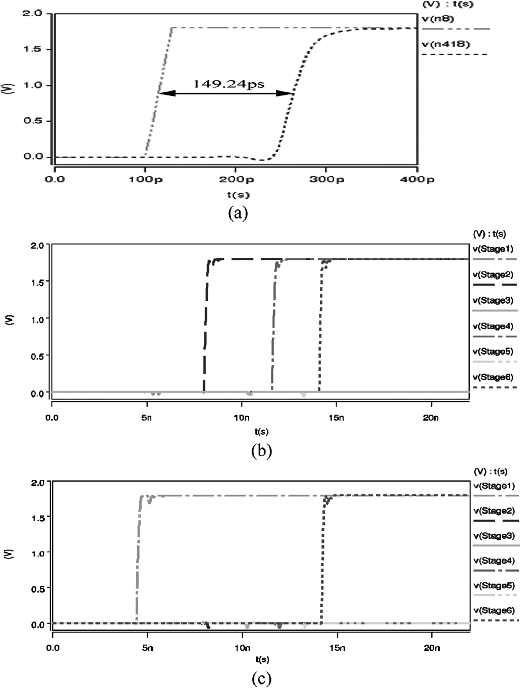
\includegraphics[width=0.75\textwidth]{OCDM-fig9}
    \caption{Simulated waveform for delay measurement of Path 1. (a) Delay from HSPICE simulation. (b) Delay difference of the import lines. (c) Delay measurement result of PUM.}
    \label{fig:OCDM-fig9}
\end{figure}

\begin{figure}[t]
\centering
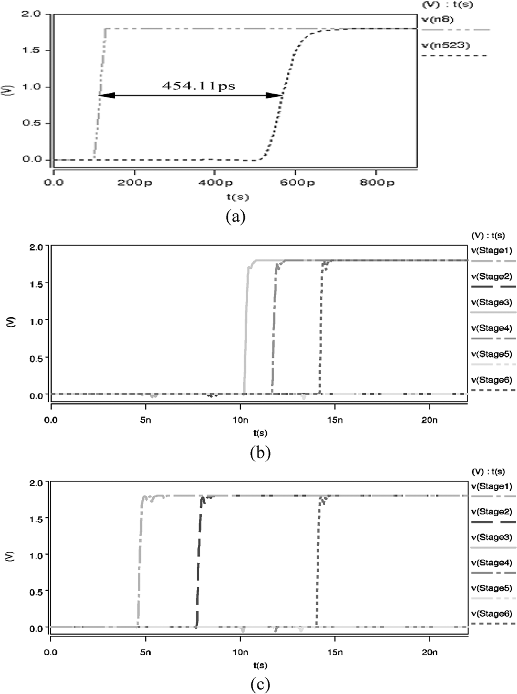
\includegraphics[width=0.75\textwidth]{OCDM-fig10}
    \caption{Simulated waveform for delay measurement of Path 2. (a) Delay from HSPICE simulation. (b) Delay difference of the import lines. (c) Delay measurement result of PUM.}
    \label{fig:OCDM-fig10}
\end{figure}

\subsubsection{Experiment III}
The circuit parameters are apparently prone to fluctuations caused by the significant process variations in sub-micro technologies. Hence the delays of circuit paths, import lines, and the delay ranges of the delay stages in OCDM circuit are thus unavoidable to suffer from undesirable variations. In this experiment, HSPICE Monte Carlo simulations are conducted to analyze the effectiveness of the proposed on-chip path delay measurement method in the presence of process variations. It is well known that the gate length variation poses a dominant impact on the gate delay \cite{nassif2000delay} \cite{agarwal2003statisticalc}. In our analysis, the inter-die and intra-die gate length variations are considered to have Gaussian distributions, $N(\mu_{L}, \delta_{1})$ and $N(\mu_{L}, \delta_{2})$, respectively \cite{wang2008path} \cite{tayade2008small}. The $\delta_{1}$ and $\delta_{2}$ represent the standard deviations of gate length for inter-die and intra-die variations respectively, while $\mu_{L}$ represents the transistor channel length obtained from the typical technology library.

Figure \ref{fig:OCDM-fig11}(a) and Figure \ref{fig:OCDM-fig11}(b) show the waveform of delay measurement results for Path1 and Path2, which are obtained from 50 Monte Carlo iterations considering both intra-die and inter-die variations. The variations considered in theMonte Carlo simulations are $3\delta_{1}=0.05\mu_{L}$ and $3\delta_{2}=0.05\mu_{L}$.

\begin{figure}[t]
\centering
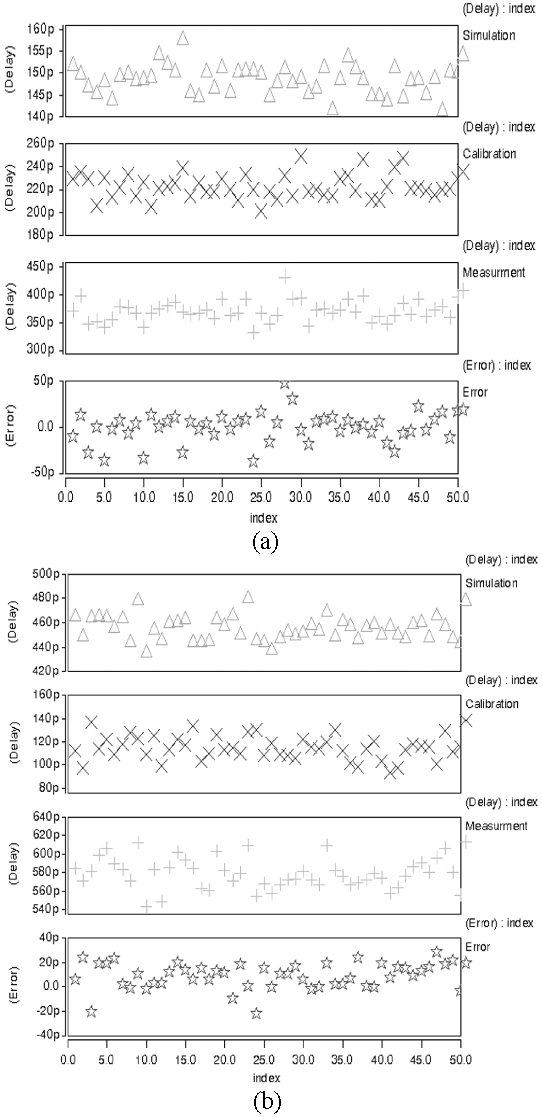
\includegraphics[width=0.6\textwidth]{OCDM-fig11}
    \caption{Simulated waveform for delay measurement obtained from 50 Monte Carlo iteration with $3\delta_{1}=0.05\mu_{L}$ and $3\delta_{2}=0.05\mu_{L}$ (a) for Path1 (b) for Path2.}
    \label{fig:OCDM-fig11}
\end{figure}


The panel indicated as Simulation in Figure \ref{fig:OCDM-fig11}(a) shows the simulation delay results of Path1 using HSPICE Monte Carlo method. Note that the delay of Path1 without considering process variations is 149.24 ps as shown in Figure \ref{fig:OCDM-fig9}. The delays of the import lines for feeding the start and end transitions of Path1 into the OCDM circuit would also be impacted by process variations. The panel indicated as Calibration in Figure \ref{fig:OCDM-fig11}(a) shows the delay measurement results of the delay difference between the corresponding import lines. The panel indicated as Measurement in Figure \ref{fig:OCDM-fig11}(a) shows the delay measurement results of Path1 without considering the delay difference of import lines $P_{2}$ and $P_{3}$. The panel indicated as Error in Figure \ref{fig:OCDM-fig11}(a) shows the errors between the delay measurement and simulation results for Path1 in the 50 Monte Carlo iterations, respectively. Likewise, the corresponding experimental results for Path2 are shown in Figure \ref{fig:OCDM-fig11}(b). Clearly, as shown in Figure \ref{fig:OCDM-fig11}, the error of path delay measurement conducted by the proposed scheme is very small, which demonstrates the effectiveness of the proposed path delay measurement scheme under process variations.


Figure \ref{fig:OCDM-fig12}(a) and Figure \ref{fig:OCDM-fig12}(b) show the Monte Carlo simulation results of delay measurement for Path1 and Path2 considering $3\delta_{1}=0.1\mu_{L}$ and $3\delta_{2}=0.1\mu_{L}$. It is clearly shown from Figure \ref{fig:OCDM-fig12} that although much larger delay variations are occurred as compared to the case in Figure \ref{fig:OCDM-fig11}, the error of path delaymeasurement results conducted by the proposed scheme is still very small, all within
the range of 50 ps.

\begin{figure}[t]
\centering
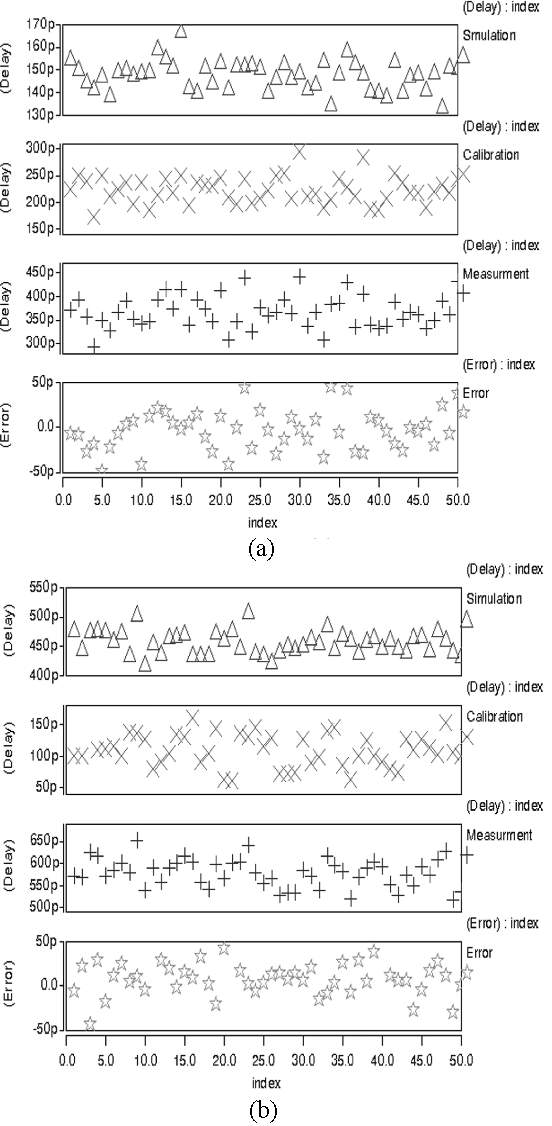
\includegraphics[width=0.6\textwidth]{OCDM-fig12}
    \caption{Simulated waveform for delay measurement obtained from 50 Monte Carlo iteration with $3\delta_{1}=0.1\mu_{L}$ and $3\delta_{2}=0.1\mu_{L}$, (a) for Path1 (b) for Path2.}
    \label{fig:OCDM-fig12}
\end{figure}


\subsubsection{Area and Timing Overhead}
In this experiment, the proposed path delay measurement architecture was incorporated into several IWLS 2005 full-scanbased benchmark circuits to evaluate its hardware and timing overheads. The area overheads reported in this paper are obtained by using a commercial synthesis tool targeting the SMIC \SI{0.18}{\micro\metre} CMOS technology. The benchmark circuits’ profiles and the area overhead of the proposed approach incorporated into the benchmark are presented in Table \ref{tab:area-overhead}. The circuit’s name of the benchmarks and the numbers of the flip-flops are given in column 1 and column 2, respectively. The column under “Circuit Area (\SI{}{\micro\metre^{2}})” reports the area of the benchmark circuits without implementing the proposed delay measurement architecture, while the sub-columns “Total”, “NoComb”, “Comb” represent the corresponding total, sequential, and combinational part’s area, respectively. Due to the different delaymeasurement requirements pursued by test experts, various path sets with totally different sizes and path delays may be selected for delay measurement. In this paper, we only focus on the delay measurement architecture rather than how to select the circuit paths targeting for delay measurement. Hence, we evaluate the area overheads of the proposed delay measurement architecture considering different numbers of path endpoints, even in the worst case where all the flip-flops are acted as the endpoints of paths for delay measurements. The columns “20\%M”, “60\%M”, and “100\%M” represent three cases in which 20\%, 60\%, and 100\% of the flip-flops are the endpoints of paths under measurements. For each of these flip-flops, a multiplexer is added to calibrate the delay difference of import lines. The sub-columns “Area ( \SI{}{\micro\metre^2} )” and “Area (\%)” under the three cases report the area overhead of the proposed delay measurement architecture and its percentage against that of the original benchmark circuit. 

\begin{table}[]
  \scriptsize
  \caption{Area Overhead of The Proposed Delay Measurement Architecture} \label{tab:area-overhead}
      \begin{tabular}{@{}l|c|ccccccccc}
          \hline
          \multirow{3}{*}{Circuit} & \multirow{3}{*}{\# of FFs} & \multicolumn{3}{c|}{Circuit Area (\SI{}{\micro\metre^2})}                                                            & \multicolumn{6}{c}{Area Overhead of the Proposed Scheme}                                                                                                                                                                         \\ \cline{3-11} 
                                   &                            & \multicolumn{1}{c}{\multirow{2}{*}{Total}} & \multicolumn{1}{c}{\multirow{2}{*}{NoComb.}} & \multicolumn{1}{c|}{\multirow{2}{*}{Comb.}} & \multicolumn{2}{c|}{20\%M}                                                       & \multicolumn{2}{c|}{60\%M}                                                       & \multicolumn{2}{c}{100\%M}                                 \\ \cline{6-11} 
                                                            &                            &                         &                          &  \multicolumn{1}{c|}{}                      & \multicolumn{1}{c}{Area(\SI{}{\micro\metre^2})} & \multicolumn{1}{c|}{Area(\%)} & \multicolumn{1}{c}{Area(\SI{}{\micro\metre^2})} & \multicolumn{1}{c|}{Area(\%)} & \multicolumn{1}{c}{Area(\SI{}{\micro\metre^2})} & Area(\%) \\ 
          \hline
                                                            des\_perf                & 8808                       & \multicolumn{1}{c}{1196203}                & \multicolumn{1}{c}{585978}                   & \multicolumn{1}{c|}{610225}                 & \multicolumn{1}{c}{57037}                       & \multicolumn{1}{c|}{4.77\%}   & \multicolumn{1}{c}{150794}                      & \multicolumn{1}{c|}{12.61\%}  & \multicolumn{1}{c}{244550}                      & 20.44\%  \\ 
                                                            wb\_conmax               & 578                        & \multicolumn{1}{c}{230776}                 & \multicolumn{1}{c}{48243}                    & \multicolumn{1}{c|}{182533}                & \multicolumn{1}{c}{13235}                       & \multicolumn{1}{c|}{5,74\%}   & \multicolumn{1}{c}{19388}                       & \multicolumn{1}{c|}{8.40\%}   & \multicolumn{1}{c}{25540}                       & 11.07\%  \\ 
                                                            aes\_core                & 530                        & \multicolumn{1}{c}{202325}                 & \multicolumn{1}{c}{38699}                    & \multicolumn{1}{c|}{163626}                 & \multicolumn{1}{c}{12980}                       & \multicolumn{1}{c|}{6.42\%}   & \multicolumn{1}{c}{18621}                       & \multicolumn{1}{c|}{9.20\%}   & \multicolumn{1}{c}{24263}                       & 11.99\%  \\ 
                                                            pci\_bridge32            & 3313                       & \multicolumn{1}{c}{396500}                 & \multicolumn{1}{c}{264226}                   & \multicolumn{1}{c|}{132274}                 & \multicolumn{1}{c}{27792}                       & \multicolumn{1}{c|}{7.01\%}   & \multicolumn{1}{c}{63057}                       & \multicolumn{1}{c|}{15.90\%}  & \multicolumn{1}{c}{98322}                       & 24.80\%  \\ 
                                                            ac97\_ctrl               & 2229                       & \multicolumn{1}{c}{237119}                 & \multicolumn{1}{c}{174892}                   & \multicolumn{1}{c|}{62227}                  & \multicolumn{1}{c}{22022}                       & \multicolumn{1}{c|}{9.29\%}   & \multicolumn{1}{c}{45749}                       & \multicolumn{1}{c|}{19.29\%}  & \multicolumn{1}{c}{69475}                       & 29.30\%  \\ 
                                                            mem\_ctrl                & 1126                       & \multicolumn{1}{c}{158606}                 & \multicolumn{1}{c}{92866}                    & \multicolumn{1}{c|}{65740}                  & \multicolumn{1}{c}{16152}                       & \multicolumn{1}{c|}{10.18\%}  & \multicolumn{1}{c}{28138}                       & \multicolumn{1}{c|}{17.74\%}  & \multicolumn{1}{c}{40123}                       & 25.30\%  \\ 
                                                            usb\_funct               & 1741                       & \multicolumn{1}{c}{242305}                 & \multicolumn{1}{c}{127228}                   & \multicolumn{1}{c|}{115077}                 & \multicolumn{1}{c}{1945}                        & \multicolumn{1}{c|}{8.02\%}   & \multicolumn{1}{c}{37957}                       & \multicolumn{1}{c|}{15.66\%}  & \multicolumn{1}{c}{56489}                       & 23.31\%  \\ 
                                                            systemcaes               & 670                        & \multicolumn{1}{c}{139789}                 & \multicolumn{1}{c}{55894}                    & \multicolumn{1}{c|}{83895}                  & \multicolumn{1}{c}{13725}                       & \multicolumn{1}{c|}{9.82\%}   & \multicolumn{1}{c}{20857}                       & \multicolumn{1}{c|}{14.92\%}  & \multicolumn{1}{c}{27989}                       & 20.02\%  \\ 
          \hline
      \end{tabular}
  \end{table}


As is clearly shown in the Table \ref{tab:area-overhead}, even in the worst case, the hardware overhead of the proposed delay measurement architecture can be acceptable. In practice, this scenario may be much more optimistic. For instance, Table \ref{tab:des-perf} reports the hardware overhead of the proposed architecture for des perf benchmark circuit, where all the critical paths that can be single-path sensitized are selected for delay measurement. As shown in Table \ref{tab:des-perf}, the clock period of the des perf circuit is synthesized to 2.6 ns by using a commercial synthesis tool, which guarantees a slack of 10\% the clock period for the longest path of the circuit under static timing analysis. The number of the selected critical internal paths is 1164, which is obtained by using a commercial timing analysis tool by specifying the path slack of which is less than 20\% of the clock period. For the selected critical internal paths, the number of paths that can be detected under the single path sensitization criterion is 779, which is obtained by using a commercial test generation tool and can then be sensitized for delay measurement. Clearly, multiple critical paths may be ended at the same endpoint. The number of endpoints for these paths suitable for delay measurement is 253. Therefore, only 253 endpoints should be inserted with the multiplexers to support the proposed delay measurement architecture. The area overhead of the whole proposed delay measurement architecture is \SI{116892}{\micro\metre^2}, and its percentage against that of the original benchmark circuit is only 1.41\%.

\begin{table}[]
  \begin{center}
    \setlength{\tabcolsep}{4mm}
    \scriptsize
    \caption{Experiment Results of DES\_Perf Circuit} \label{tab:des-perf}
    \begin{tabular}{@{}lc}
        \toprule
        Benchmark                       &  \ Des\_perf \  \\ 
        \midrule
        \# of FFs                       & 8808      \\ 
        Clock Period(ns)                & 2.6       \\ 
        \# of circuit critical paths    & 1164      \\ 
        \# of single path sensitization & 779       \\ 
        \# of critical endpoint         & 253       \\ 
        Area Overhead(\SI{}{\micro\metre^2})              & 16892     \\ 
        Area Overhead (\%)              & 1.41\%    \\ 
        \bottomrule
    \end{tabular}
  \end{center}
\end{table}


Due to the application of the proposed delay measurement architecture, the delay of circuit paths may be impacted. Hence, the timing overhead of the delay measurement architecture to the critical path, which impacts the circuit performance, should be evaluated. Table \ref{tab:timing-overhead} evaluates the timing impact of the proposed delay measurement architecture to the delay of the longest circuit internal path in each benchmark circuit. The experimental circuit’s names and clock domains are listed in the column 1 and column 2, respectively. The columns under “Longest internal path delay (before)”and “Longest internal path delay (after)” represent the delays of the longest internal path before and after the incorporation of the delay measurement architecture for the considered clock domain. The column under “Delay increase” represents the delay increase of the longest path caused by incorporation of the proposed architecture. The column under “Timing overhead” represents the percentage of delay increase against the delay of the longest internal path before incorporation of the delay measurement architecture. As shown in Table \ref{tab:timing-overhead}, the timing impact of the proposed delay measurement architecture to the sample circuit is less than 0.7\% of the longest internal delay and can be negligible.

\begin{table}[]
  \begin{center}
    \setlength{\tabcolsep}{1mm}
    \scriptsize
    \caption{Timing Overhead}\label{tab:timing-overhead}
    \begin{tabular}{@{}llcccc}
        \toprule
        Circuit       &  \ clock domain \      & \begin{tabular}[c]{@{}c@{}}Longest circuit internal \\ path delay (before) (ns)\end{tabular} & \begin{tabular}[c]{@{}c@{}}Longest circuit internal \\ path delay (after) (ns)\end{tabular} & \begin{tabular}[c]{@{}c@{}}Delay \\ increase (ps)\end{tabular} & \begin{tabular}[c]{@{}c@{}}Timing \\ Overhead(\%)\end{tabular} \\ 
        \midrule
            des\_perf     & clk              & 2.0280                                                                                       & 2.0377                                                                                      & 9.7                                                            & 0.48\%                                                         \\ 
            wb\_conmax    & clk\_i           & 1.9256                                                                                       & 1.9644                                                                                      & 11.8                                                           & 0.60\%                                                         \\ 
            aes\_core     & clk              & 2.7504                                                                                       & 2.7588                                                                                      & 8.4                                                            & 0.31\%                                                         \\ 
            pci\_bridge32 & pci\_clk\_i      & 1.7575                                                                                       & 1.7656                                                                                      & 8.1                                                            & 0.46\%                                                         \\ 
            ac97\_ctrl    & clk\_i           & 2.0684                                                                                       & 2.0790                                                                                      & 10.6                                                           & 0.51\%                                                         \\ 
            mem\_ctrl     & clk\_i           & 2.0788                                                                                       & 2.0931                                                                                      & 14.3                                                           & 0.69\%                                                         \\ 
            usb\_funct    & phy\_clk\_pad\_i & 1.8180                                                                                       & 1.8261                                                                                      & 8.1                                                            & 0.44\%                                                         \\ 
            systemcaes    & clk              & 3.0745                                                                                       & 3.0813                                                                                      & 6.8                                                            & 0.22\%                                                     \\ 
            \bottomrule
    \end{tabular}
  \end{center}
\end{table}

\subsubsection{Comparison A}
To compare with previous works, the delay measurement circuits using the proposed OCDM method and the method from \cite{datta2004chip} which employed a modified VDL with equal delay range value in each stage are implemented respectively. Table V compares the experimental results of the two methods. Note that the proposed OCDM circuit needs only 3.3\% of the delay stages to achieve even larger maximum delay measurement range compared to the delay measurement circuit using the method from \cite{datta2004chip}, while the delay measurement resolution of the proposed OCDM circuit is only 49\% of that for the delay measurement circuit using the method from \cite{datta2004chip}. As mentioned earlier, when the delay measurement is completed, the values stored in the flip-flops of the OCDM circuit should be shifted out serially using slow shift clock. If we assume the frequency of shift clock is 1GHz, then the time for scanning out themeasurement values is only 8ns for the proposed OCDM circuit, but is up to 245ns for the delay measurement circuit using the method from \cite{datta2004chip}.


\begin{table}[]
  \begin{center}
    \setlength{\tabcolsep}{1mm}
    \scriptsize
    \caption{Measurement Circuit Comparison}\label{tab:cmp}
    \begin{tabular}{lccc|ccc}
        \hline
        \multirow{2}{*}{Circuit} & \multirow{2}{*}{\begin{tabular}[c]{@{}c@{}}Stage \\ Numbers\end{tabular}} & \multirow{2}{*}{ \ Resolution \ } & \multirow{2}{*}{\begin{tabular}[c]{@{}c@{}}Maximum \\ Measurement Range\end{tabular}} & \multicolumn{3}{c}{Area (um2)}                                                    \\  \cline{5-7}
                                     &                                                                           &                             &                                                                                       & \multicolumn{1}{c}{Combinational} & \multicolumn{1}{c}{No Combinational} & Total \\ 
                                  \hline
                                     Proposed OCDM            & 8                                                                         & 6.62ps                      & 3295ps                                                                                & \multicolumn{1}{c}{9547}          & \multicolumn{1}{c}{612}              & 10159 \\ 
                                     {\cite{datta2004chip}}                 & 245                                                                       & 13.45ps                     & 3295ps                                                                                & \multicolumn{1}{c}{26894}         & \multicolumn{1}{c}{18744}            & 45638 \\ 
                                     \hline
    \end{tabular}
  \end{center}
\end{table}

The area overheads of the two delay measurement circuits are obtained using a commercial synthesis tool. It can be seen that the combinational, non-combinational, and the total area overheads of the proposed OCDM circuit are only 35.5\%, 3.3\%, and 22.3\% of that for the delay measurement circuit using the method from \cite{datta2004chip} respectively. It seems unfair to compare only the hardware overhead of the OCDM circuit of the proposed delay measurement architecture with the delay measurement circuit using themethod from \cite{datta2004chip} without considering the hardware overhead of the insertion of multiplexers at the endpoints of the PUMs. However, it should be noted that the OCDM circuit provides the same path delay measurement ability with that of the method from \cite{datta2004chip}, while the purpose of the insertion for 2-to-1 multiplexers to the end points of the PUMs is to calibrate the delay difference of import lines. Thereby, a higher precision of delay measurement results for the PUMs can be obtained by the proposed method as compared to the method from \cite{datta2004chip}.

\subsubsection{Comparison B}
By considering the delay difference of the import lines in the proposed scheme, and considering the returning loop delay in the Path-RO scheme \cite{wang2008path}, both the proposed scheme and the Path-RO scheme can provide a high precision for path delay measurement. However, as compared to the Path-RO technique, the proposed technique provides a more effective way to measure the delay of a path. This is mainly due to the following reasons.

1) A multiplexer is required to be inserted into the critical PUM in the Path-RO technique, which reduces the speed of high performance circuit. Clearly, in the proposed path delay measurement architecture, no extra cell has to be inserted in the PUM, while only a small overload from one input of the multiplexer is added in the PUM. Hence, the proposed technique has a weak impact to the delay of a critical path as compared to the Path-RO technique.

2) The Path-RO technique can only measure either the delays of paths that begin at a clocked flip-flop or the delays of paths that end at this clocked flip-flop. The reason is that the flip-flop which is the start point of the PUM has to be modified to a calibration launch flip-flop (CLFF), while the flip-flop which is the end point of the PUM has to be modified to a calibration capture flip-flop (CCFF) with a different circuit structure. However, the delay of each circuit path chosen for delay measurement can be obtained by the proposed on-chip path delay measurement technique.

3) In order to measure the delay of a path by using the Path-RO technique, one and two extra multiplexers are required to be added in the flip-flops which are stood at the input and output of the PUM, respectively. However, only one extra multiplexer is required to be added for the flip-flop which is the endpoint of the PUM in the proposed path delay measurement technique. Hence, the proposed method suffers from a significant lower hardware overhead as compared to the Path-RO technique.

4) By using the Path-RO technique, only the delay of a path on which the number of inverting logics is odd can be measured due to the use of the oscillation technique. Otherwise, one inverter is required to be added to the PUM, which will further increase the design complexity to the path delay measurement architecture. Moreover, the delay of the returning loop might not be calibrated to a clock period because the first requirement of the calibration process is to assure that the PUM is configured to be able to oscillate. Hence, the precision of the path delay measurement would be influenced. Clearly, no such extra restrictions are posed into the proposed on-chip path delay measurement technique when measuring the delay of a chosen circuit path.

\subsection{Discussion}
In this paper, we have presented a novel on-chip path delay measurement technique for timing characterization and silicon debug. In the proposed OCDM circuit, the delay range of each delay stage is set to increase by a factor of two gradually from the last to the first delay stage. In addition, by conducting delay compensation, both improved delay measurement resolution and measurement precision can be provided when compared to the previous VDL based delay measurement schemes. The delay difference of the import lines for feeding the start and end transitions of the PUM into the OCDM circuit is also considered in the proposed technique, which can further provide a high precision for path delay measurement. Experimental results show that the proposed on-chip path delay measurement scheme works well. A small quantity of delay stages in OCDM circuit can obtain a large delay measurement range, and hence can provide a significant reduction in delay measurement time. Moreover, the area overhead of the proposed method is also significantly reduced as compared to previous works.

\section{Lifetime Fault-Tolerant Circuit Design}
In the past decades, the device and reliability communities have devoted much efforts to lifetime projection \cite{Sony}\cite{Atmel}, but less to design for lifetime reliability. This situation would be changed because the lifetime reliability is seriously challenged by the aggressive technology scaling \cite{degradation_05}\cite{ITRS_PIDS07}. One of the major impending (above 22nm) challenges comes from MOS transistor wearout \cite{ITRS_PIDS07}; NBTI (negative bias temperature instability) and TDDB (time dependent dielectric breakdown) draw the most attentions over a wide variety of transistor aging mechanisms \cite{ITRS_PIDS07}. Both aging mechanisms can gradually degrade the performance of transistors over time \cite{agarwal2007circuit}\cite{Self-calibrating_07} due to elevated threshold voltage \cite{NBTI_Impact05}\cite{wang2007impact} or degraded integrity of gate oxide \cite{OB_Invert_03}\cite{Impact_BD_04}\cite{Gate-oxide-breakdown-07}.

To guarantee the chips' lifetime reliability, a common practice is reserving conservative timing margin---just like that for process variations \cite{ParameterVariations_DAC03}. However, the effectiveness of such approaches is diminishing, given that up to 10-20\% guardband has to be reserved to safely accommodate the aging-induced performance degradation---which can even offset the performance benefit from one-generation of technology advancement.

Many researches have been conducted at different levels: device level \cite{DynamicNBTI_03}\cite{Modeling-and-minimization_06}, circuit level \cite{Compact-Modeling_07}\cite{wang2007impact}, and (micro)architecture level \cite{Reliability-Aware_04}\cite{Penelope_07}\cite{Framework_DSN07}. Particularly, Blome et al. proposed an online wearout detection approach through sensing the aging-induced delay \cite{Self-calibrating_07}. Agarwal et al., based on the same observation, proposed a sensor design dedicated for aging failure prediction \cite{agarwal2007circuit}. Yan et al. presented a more versatile and cost efficient sensor design \cite{SVFD_09} which can also be used for aging detection.

Although the prior sensor designs prepare a ground for aging-aware designs, few researches are conducted so far to study how to effectively use them; this work aims to serve this purpose. The lifetime of a chip is governed by the "weakest-link principle"---usually only a minority of transistors suffer large aging degradation reflected in excessive path delay. The aging sensors can capture this change; however, previous solutions such as turning voltage and/or frequency \cite{Reliability-Aware_04}, reducing individual core utilization \cite{Facelift_08}, and duplicating hardware resources \cite{srinivasan2005exploiting}\cite{WearoutRecovery_08} do not use such fine-grained detection capability sufficiently. Although those architecture- and application-level approaches are somewhat effective to remedy the aged chips, these coarse-grained solutions trading either performance or hardware resources for lifetime may be far from efficient due to the blindness to the minority of fine-grained "weakest links" which can be identified by the aging sensors.


Above analysis motivates us to propose a new approach to exploiting fine-grained aging adaptability. Unlike those coarse-grained approaches, the fine-grained approach can cope with the "weakest-links" more locally and efficiently, thereby making it possible to improve lifetime reliability while without compromising with the architectural performance and coarse-grained hardware resources. In particular, we make three contributions:
\begin{enumerate}
\item We propose ReviveNet, a hardware-implemented aging-aware and self-adaptive architecture, to improve lifetime reliability. Aging-awareness is realized by deploying dedicated aging sensors, and "self-adaptive" is achieved by employing a group of synergistic adaptation agents.

\item To support ReviveNet, we present a localized timing adaptation mechanism, with which the aged critical paths can be locally coped with. The fine-grained adaptability results from timing imbalance between consecutive timing paths. The lifetime can be extended significantly through exploiting such "path-grained" adaptability.

\item We propose an evaluation model to quantitatively study the ReviveNet-enhanced reliability.
\end{enumerate}

The effectiveness of ReviveNet has been evaluated through incorporating it into an industrial pipelined floating-point co-processor. Experimental results show that ReviveNet can improve the MTTF by 48.7\% without compromising with architectural performance, only at about 9.5\% area and small power overhead.


\subsection{Aging Symptoms and Aging Sensors}
The aging-induced delay is a suitable symptom candidate \cite{Self-calibrating_07} \cite{agarwal2007circuit} \cite{failure_prediction2_08}. For example, Blome et al. took the TDDB induced delay as the symptom for wearout detection \cite{Self-calibrating_07}. Agarwal. et al, took the NBTI induced delay as the symptom for aging failure prediction \cite{agarwal2007circuit}\cite{failure_prediction2_08}. We also take aging delay as the symptom in this work.

Aging-awareness can be realized by employing some dedicated aging sensors. The fundamental working principle of sensors is on-line delay fault detection. The only difference between the aging sensing and traditional delay fault detection is that the former takes place in a safe timing interval called "Guard band" \cite{agarwal2007circuit}, while the latter takes place in the interval after the effective clock edge called "Detection slack" \cite{SVFD_09}. As Figure \ref{agingdelay} shows, initially, in fresh state, no signal transitions occur in guard band, but after suffering form aging, some transitions could be delayed into guard band. Since the signal should have been stabilized before entering the guard band, we call the event of such a ``faulty" transition in guard band as a Stability Violation \cite{SVFD_09}. It is worthy to note that the detected aging delay, unlike conventional delay faults, won't cause any timing fault (a.k.a. Timing violation).

\begin{figure}[t]
\centering
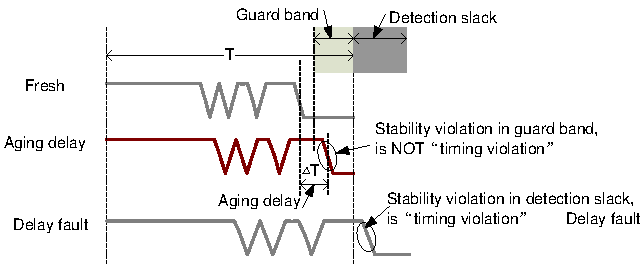
\includegraphics[width=0.6\textwidth]{fig2-12}%{agingdelay.eps}
   \caption{The timing of Aging delay and delay fault}\label{agingdelay}
\end{figure}

\begin{figure}[t]
\centering
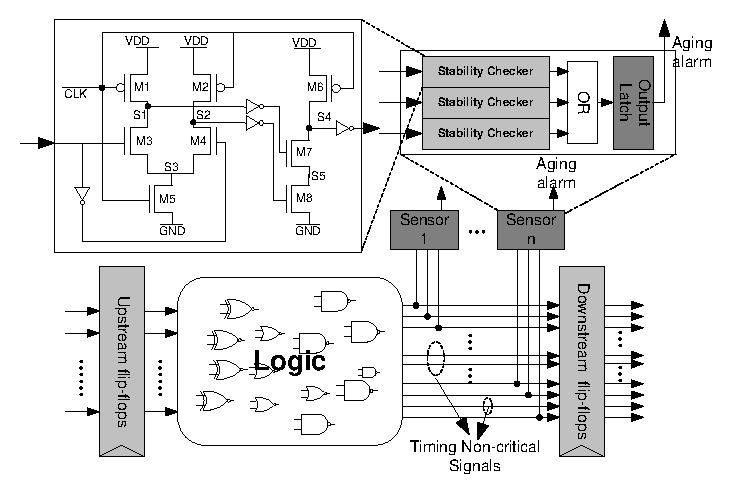
\includegraphics[width=0.65\textwidth]{fig2-13}%{sensorsetup.eps}
\vspace{-0.5cm}
   \caption{Sensor setup}\label{setupsonsor}
\end{figure}

The detection for aging delay is actually to detect the stability violations in guard band. We can use stability checker---the key component in aging sensor---to fulfill this purpose. The basic stability checker can be derived from a sensing circuit for on-line delay fault detection, in which the signal integrity is verified by a pair of consistent charge/discharge nodes, the delay transitions will trigger one of the charged nodes to be discharged and thereby causes state inconsistence between them. More specifically, as shown in Fig \ref{setupsonsor}, during precharge period, both nodes $S1$ and $S2$ in the stability checker are charged up to HIGH. The circuit starts evaluation when entering the guard band; one of the two nodes is pulled down, while the other one floats at HIGH because the gate signal of M3 is always complemented with that of M4. Hence, the node $S1$ and $S2$ are always exclusive during fault-free time, which will make the node $S4$ stick to HIGH because the high-impedance path between S4 and GND always exists. When aging delay happens, the stability violation will trigger the discharge of the node that has charged up to HIGH. Eventually both nodes are discharged, and thereby the node S4 is pull down to LOW---which flags aging delay being detected. Please refer to \cite{SVFD_09} for more details.

One sensor consists of multiple stability checkers, one wide dynamic OR gate, and one output latch \cite{SVFD_09}. To reduced overhead, multiple stability checkers share one output latch through a wide dynamic OR gate, as shown in Figure \ref{setupsonsor}.

The aging sensors are deployed to monitor critical paths. As an example, Figure \ref{setupsonsor} shows a setup for a stage of logic, where each sensor handles three signals. If some aged transistors in the logic or upstream flip-flops result in stability violations in the guard band---aging delay, the corresponding sensors can tell that an aging failure is impending.

With the "awareness" of aging, the next essential problem is how to accommodate the impending aging failures indicated by these alarms. The ReviveNet aims to address this problem.

\subsection{Lifetime Fault-tolerant Architecture}

Figure \ref{syntop} illustrates the ReviveNet architecture. Each stage is monitored by a set of periodically-invoked aging sensors. The adaptation to each stage is implemented with a set of adaptation agents which are fed by not only the local stage's aging sensors but also the next stage's agents, thereby enabling bidirectional adaptation\,---\,\emph{backward timing adaptation} (BTA) and \emph{forward timing adaptation} (FTA).  BTA is using the $(K+1)$st stage's timing slack to accommodate the aging emergencies in the $K$th stage, while FTA is using the $(K-1)$st stage's slack to accommodate the emergencies in the $K$th stage.  With the bidirectional adaptation mechanism, ReviveNet offers more adaptation freedom and performs more effectively.


\begin{figure}[t]
\centering
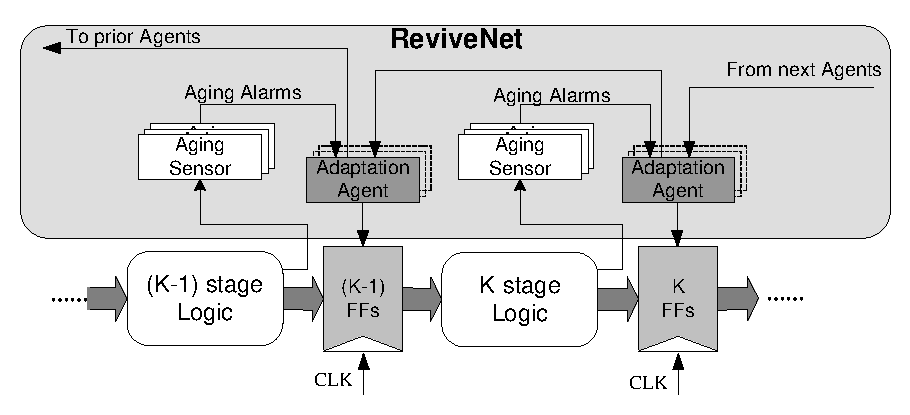
\includegraphics[width=0.65\textwidth]{fig2-14}%{revivenet.eps}
   \caption{ReviveNet architecture}\label{syntop}
\end{figure}

\begin{figure}[h]
 \centering
  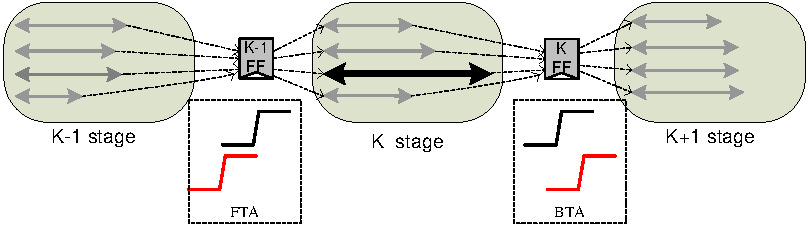
\includegraphics[width=0.7\textwidth]{fig2-15}%{ba_fa.eps}
  \caption{Example of adaptation}\label{ba_fa}
\end{figure}

Let's explain the basic idea of ReviveNet with a simple example. Figure \ref{ba_fa} shows a part of a pipeline, where each arrow denotes a timing path and the length of it represents corresponding delay; in particular, the critical path in the middle stage is denoted by a bold arrow. After experiencing some aging, suppose that the delay of the critical path is going to exceed the clock period---an impending aging failure, an aging sensor monitoring this path detects the impending failure \cite{agarwal2007circuit}\cite{SVFD_09} and flags an aging alarm; then, three local adaptation options can be enabled to tolerate this aging delay: 1) backward skew the clock of $K$th flip-flop---BTA, 2) forward skew the clock of $(K-1)$st flip-flop---FTA, or 3) both FTA and BTA. The specific adaptations are governed by a finite state machine, referred to agent.

The above conceptual example can just convey a very basic idea of ReviveNet; we can gain more insights into the ReviveNet's operations and underling design tradeoffs by answering the following questions:

{\bf 1) Why are BTA and FTA feasible?}

Clearly, BTA or FTA can help tolerate the aging delay of the target critical path only if there is timing imbalance between the corresponding paths, i.e. all upstream paths of $(K-1)$st flip-flop, or all downstream paths of $K$th flip-flop are non-critical. We call such imbalance as path-grained (or, localized) adaptability. We will use a case study (Section \ref{sec:investigation} investigation) to show that the potential of such localized adaptability, which ReviveNet aims to exploit, is quite attractive.

{\bf 2) Where the sensors and agents should be deployed?}

This problem is trivial if both the critical paths and aging impacts can be well-predicted: every critical path that is prone to suffer aging impacts should be monitored by a sensor. Unfortunately, though the critical paths can be somewhat distinguished from non-critical paths with some sophisticated SSTA (statistical static timing analysis) approaches, many researches have been evident that the aging degree of individual transistor highly depends on the physical geometries, defect density and the stress states during working mode. In other words, the aging degree of individual transistor is highly unpredictable; hence it seems hopeless to identify the aging-prone critical paths. We take an engineering way to tackle this problem: conservatively put all critical paths under monitor. Thought it is not an theoretically optimum option, the experimental results show that such engineering way is still cost-efficient (Section \ref{section_casestudy} Case Study).

Deploying agents is based on the sensors deployment and specific circuit topology. The detail can be found in (Section \ref{deploy_agentsensor} Deploy Agents and Sensors).

{\bf 3) What's the adaptation logic of agents?}

Usually, one sensor is able to monitor multiple critical paths to reduce the implementation overhead. The side-effect is decreased "resolution"---when a sensor flags an aging alarm, the agent actually cannot immediately recognize that which path (or paths) causes this alarm; hence the agent needs to follow a policy to efficiently identify the root of the alarm. Given that the aging is a progressive process and thus does not need to be in realtime accommodated, we propose a round-robin trial adaptation mechanism---the agent travels across a set of prioritized adaptation states to track back the source of the alarm and then tries the best to accommodate it (Section \ref{section_rrta} RRTA).


{\bf 4) How to implement the intentional clock skew?}

The intentional skew is used to enable BTA and FTA.  One way to obtain the intentional skew is by inserting delay buffers \cite{Recycle_07}. However, the drawback of such delay-buffer based design is poor controllability. For example, suppose that during the early years of service life almost no adaptation is required, but these buffers still suffer from aging, contribute to leakage power, and so on. We propose a new implementing scheme to obtain the skewed clocks in a highly controllable way, while minimizing the side effects to the adaptation-free period (Section \ref{section_clcokgen} Clcok Gen, \ref{section_clockgate} Clock Gate).


{\bf 5) What if the infrastructure of ReviveNet, sensors and agents, fail to work due to aging?}

ReviveNet is relatively aging resistant because it does not need to be always-on; most of lifetime it is power-off. Thus, the transistors' aging rate in sensors and agents, statistically, is much slower than that in host logics. We shall give more detailed discussion in Next Section.


{\bf 6) How much extended lifetime can be achieved?}

This question is hard to answer due to lack of accurate models that capture the relationship between a variety of aging mechanisms and aging delay. To quantitatively study the MTTF (Mean-Time-To-Failure) improvement, we propose a ReviveNet-enhanced  reliability model in which the relationship is condensed to a hypothetical function $\delta$ (Section \ref{section_model} Model). Then, we instantiate the function based on the well-studied NBTI mechanism (Section \ref{section_casestudy} Case Study) to show the effect of ReviveNet, though the reliability model can also be applied to other aging mechanisms that need more intensive studies in the future. Experimental results show that up to 48.7\% MTTF improvement can be achieved.


Figure \ref{curve} qualitatively shows the ReviveNet-enhanced lifetime. When ReviveNet is too exhausted to make any effective adaptation---if any of the agents fails to accommodate an impending aging failure, the chip is judged reaching the end of lifetime. ReviveNet can also readily indicate the "incurable" failure; then, one can proactively take actions, such as replacing the aged chips, degrading the architectural performance, to minimize the impacts of failure.


\begin{figure}[t]
\centering
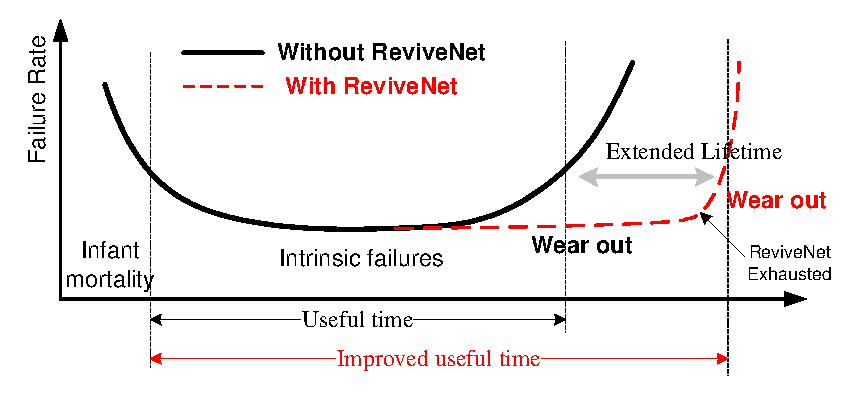
\includegraphics[width=0.55\textwidth]{fig2-16}%{curve.eps}
   \caption{Anticipated effect of ReviveNet}\label{curve}
\end{figure}

\subsection{Self-Adaptive Fault-Tolerant Pipeline}
\subsubsection{Timing Imbalance}
We describe the timing imbalance that can be exploited to tolerate the aging delay through characterizing pipeline flip-flops. A pipeline flip-flop can be categorized according to the slack values of related upstream and downstream paths. Specifically, suppose a flip-flop $FF$ serves as the end point of $m$ paths with slack values $e_1$, $e_2$, $\ldots$, $e_m$, and the start point of $n$ paths with slack values $s_1$, $s_2$, $\ldots$, $s_n$. Given a threshold, $TH$, which distinguishes the (potential) critical paths ($slack \leq TH$) from others ($slack > TH$), the flip-flop must fall into one of the four classes:

$\bullet$ Generous Flip-flop (GFF):  $\forall e_i\in$ \{$e_1$, $e_2$, $\ldots$,
$e_m$\}, s.t. $e_i>TH$, and $\forall s_j\in$ \{$s_1$, $s_2$, $\ldots$, $s_n$\}, s.t. $s_j>TH$ (say, ``Generous" with timing margin).

$\bullet$ Backward Adaptable Flip-flop (BAFF):  $\exists e_i\in$ \{$e_1$, $e_2$, $\ldots$,
$e_m$\}, s.t. $e_i\leq TH$, but $\forall s_j\in$ \{$s_1$, $s_2$, $\ldots$, $s_n$\}, s.t. $s_j>TH$.

$\bullet$ Forward Adaptable Flip-flop (FAFF):  $\forall e_i \in$ \{$e_1$, $e_2$, $\ldots$,
$e_m$\}, s.t. $e_i>TH$, but $\exists s_j\in$ \{$s_1$, $s_2$, $\ldots$, $s_n$\}, s.t. $s_j\leq TH$.

%FAFFs and BAFFs can also serve as margin providers, although in a ``unidirectional" manner.

$\bullet$ Unadaptable Flip-flop (UAFF):  $\exists e_i\in$ \{$e_1$, $e_2$, $\ldots$,
$e_m$\}, s.t. $e_i\leq TH$, and $\exists s_j\in$ \{$s_1$, $s_2$, $\ldots$, $s_n$\}, s.t. $s_j\leq TH$.


In the following cases can yield critical paths:
\begin{enumerate}
\item  start with a FAFF and end with a BAFF, or
\item  start with a FAFF and end with a UAFF, or
\item  start with a UAFF and end with a BAFF, or
\item  start with a UAFF and end with a UAFF.
\end{enumerate}

A critical path in case 2) and 3) can gain extra $TH/2$ slack (note that we let the slack-providing paths still hold at least $TH/2$ slack); that in case 1) can gain extra $TH/2+TH/2$ slack; while that in case 4) cannot gain any extra slack.


Threshold $TH$ is a key factor affecting the design tradeoffs. On one hand, the larger $TH$, the higher percentage of UAFFs, thus more critical paths will be rendered unadaptable; on the other, the larger $TH$ can facilitate more aggressive time stealing on adaptable paths. In (Section \ref{section_casestudy} Case Study), we will show that neither over-large nor over-small $TH$ can lead to an optimum design tradeoff.

\subsubsection{Self-Adaptive Design Example}\label{sec:investigation}
As a case study, the following investigates the intrinsic timing imbalance in a industry design.

\begin{figure}[t]
\centering
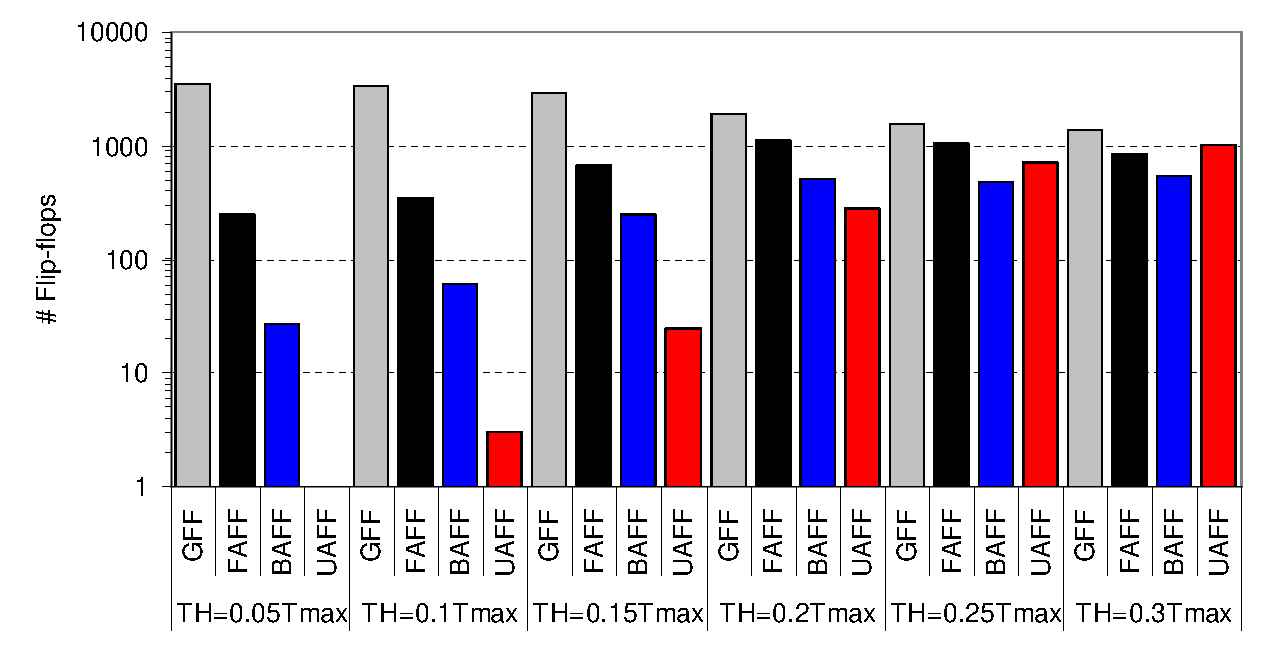
\includegraphics[width=0.75\textwidth]{fig2-17}
    \caption{Distribution of flip-flops at different $TH$}\label{ff_type}
\end{figure}

We took a pipelined FPU adopted by OpenSPARC T1 \cite{OpenSPARC_06} processor as our target circuit. This FPU is synthesized using Synopsys Design Compiler with UMC 0.18um technology, and its' path timing is analyzed with PrimeTime. We set the performance as the synthesizing priority to smooth the distribution of path delay as much as possible. The timing analysis results are shown in Figure \ref{ff_type}.

Figure \ref{ff_type} shows the breakdowns of flip-flops with different type of adaptability, under six $TH$ configurations: 0.05 ($T_{max}$), 0.1, 0.15, 0.2, 0.25, and 0.3, where $T_{max}$ represents the most critical path delay. When $TH$=0.05, all of the critical paths are adaptable due to no  UAFF appears. With $TH$ increasing, some GFFs fall into the groups of BAFFs or FAFFs, even UAFFs, but GFFs, BAFFs and FAFFs always take considerable percentage---that is the ``potential" (localized adaptability) which ReviveNet can exploit.

\subsection{Self-adaptive Agent} \label{agentdesign}
The agents are responsible for controlling the localized adaptations. Before delving into the implementation details, let's first suppose that such localized adaptations can be realized by selecting a clock from multiple available clocks skewed from each other, as Figure \ref{affs} shows. The adaptability of each flip-flop has been identified beforehand with a static timing analysis tool. The GFFs' and UAFFs' clocks are kept intact, and each FAFF's, BAFF's clock is individually controllable. Dealing with UAFFs in this way is because no favorable time margins can be exploited without hurting the timing of other critical paths, so we would rather keep them intact than take tentative adaptations which cannot guarantee any reliability benefits. A FAFF is clocked by either original clock (CLK) or forward skewed clock (FCLK) to enable FTA; a BAFF is clocked by either CLK or backward skewed clock (BCLK) to enable BTA.

\begin{figure}[t]
\centering
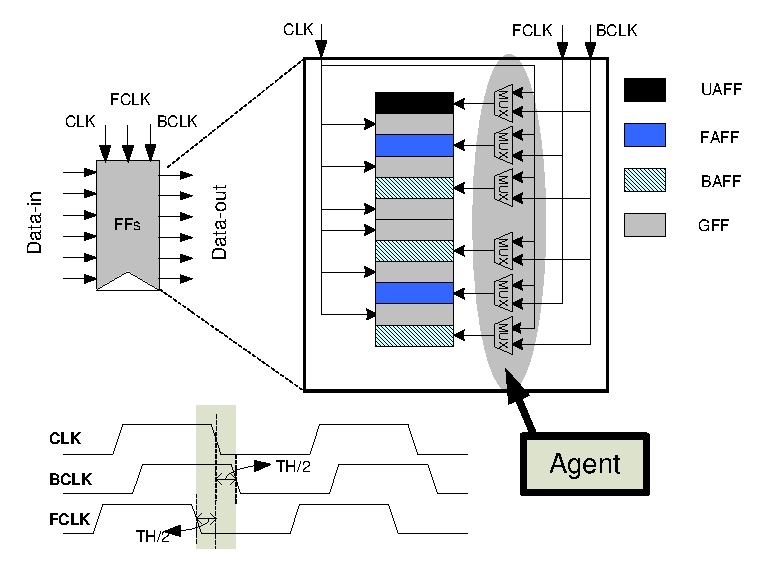
\includegraphics[width=0.7\textwidth]{fig2-18}
   \caption{Example of adaptive clock assignment (agent is responsible for
   generating the clock-steering signals)}\label{affs}
\end{figure}

In Figure \ref{affs}, suppose that a sensor is deployed to monitor all of UAFFs and BAFFs, when the sensor flags an aging alarm, how does the corresponding agent perform the clock steering? One way is to enable all of the BAFFs (the FAFFs are enabled by the next stage's agent and discussed later); however, such "brutal" way may significantly sacrifice the timing margins of the innocent paths, thus not complying with the principle of "localized adaptation". The following presents a trial-based approach to address this problem.

\subsubsection{Round-Robin Trial Adaptation (RRTA)}\label{section_rrta}

When a sensor raises an aging alarm, it could be traced back to single or multiple critical paths. Fortunately, given that circuit aging usually is a gradual process, the response of an intended adaptation does not need to be in realtime. This allowable adaptation latency can justify the proposed RRTA approach below.

RRTA performs in an "identify-then-adapt" manner. Each trial represents an adaptation state---the value of clock-steering signals of related flip-flops. Algorithm \ref{alg:rr} presents the procedure of RRTA.

%\begin{figure}[h]
%\centering
%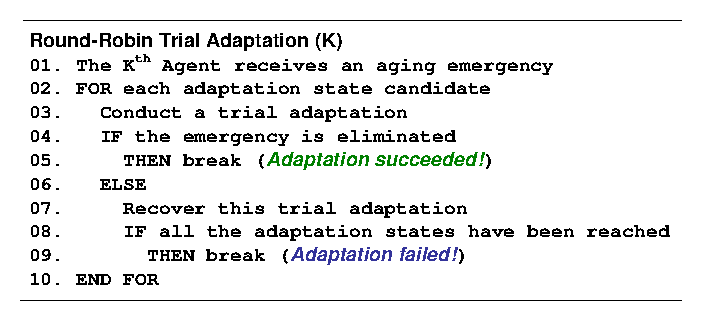
\includegraphics[width=0.7\textwidth]{fig2-19}%{rrta.eps}
%   \caption{Round-Robin Trial Adaptation}\label{rradp}
%\end{figure}

\begin{algorithm}\label{alg:rr}
  \caption{Round-Robin Trial Adaptation (K)}
  \KwData{The $K^{th}$ Agent recieves an aging emergency;}
  \For{each adaptation state candidates}{
      conduct a trial adaptation\;
      \eIf{the emergency is eliminated}
      {
        break\;\tcp*[h]{Adaptation succeeded!}
      }
      {
       Recover this trial adaptation\;
       \lIf{all the adaptation states have been reached}{break\;\tcp*[h]{Adaptation failed!}}
      }
  }
\end{algorithm}



The following clarifies how to define the set of adaptation states (related to line 1 in Algorithm \ref{alg:rr}). Generally, each agent is fed by an aging alarm and a request from another agent (as shown in Figure \ref{syntop}). For agent $A_K$ and a set of flip-flops $FF$, the aging alarms only trigger the backward adaptations to BAFFs, and the requests triggers the forward adaptations to FAFFs. The adaptation states are described with the following example.

\exmp\label{rrtaexample}  For the $K$th stage with downstream flip-flops $FF_k$=\{$f_1^k$, \ldots, $b_1^k$, $b_2^k$, $b_3^k$, $u_1^k$\} and upstream flip-flops $FF_{k-1}$=\{$f_1^{k-1}$, $f_2^{k-1}$, $f_3^{k-1}$, $f_4^{k-1}$, $b_1^{k-1}$, \ldots, $u_1^{k-1}$, \ldots\}, where $f$, $b$, and $u$ denote FAFF, BAFF, and UAFF, respectively. Agent $A_K$ and  $A_{K-1}$ handles $FF_k$ and $FF_{k-1}$, respectively. Clearly, only \{$b_1^k$, $b_2^k$, $b_3^k$\} and \{$f_1^{k-1}$, $f_2^{k-1}$, $f_3^{k-1}$, $f_4^{k-1}$\} can contribute to the $K$th stage's adaptations. Furthermore, suppose that only $f_1^{k-1}$, $f_2^{k-1}$, $f_3^{k-1}$, $f_4^{k-1}$ are related inputs to $b_1^k$, $b_2^k$, $b_3^k$. The correspondence of related FAFFs and BAFFs is easy to identify with logic core generation algorithms which has been well-studied and widely used on ATPG (Automatic Test Patten Generation) \cite{POIROT_00}.

The candidates of backward adaptation states (BAS) are denoted by $BAS$=$BAS_0$ $\cup$ $BAS_1$ $\cup$ $BAS_2$ $\cup$ $BAS_3$ where each term is a set of states corresponding to $b_1^k$, $b_2^k$, and $b_3^k$, as follows: 
{\small\begin{align}
BAS_0=\;&\{000\};            \nonumber \\
BAS_1=\;&\{001, 010, 100\};    \nonumber\\
BAS_2=\;&\{011, 101, 110\};  \nonumber \\
BAS_3=\;&\{111\}          . \nonumber
\end{align}}

$BAS_0$ is an initial state representing no adaption conducted. $BAS_1$, $BAS_2$, and $BAS_3$ represent 1-bit, 2-bit, and 3-bit backward adaptations conducting on $b_1^k$, $b_2^k$, and $b_3^k$, respectively. The agent, for example, conducts a "001" adaptation, means that BCLK for $b_3^k$ is enabled, while keeping the $b_1^k$, $b_2^k$ intact. Clearly, the perturbation level to the circuit is elevated from $BAS_1$ to $BAS_3$ because more bits adapted implies more perturbations introduced.

On the other hand, if $A_K$ receives an aging alarm, there should be another option: forward adapting the FAFFs in $FF_{k-1}$. To do so, $A_K$ needs to cooperate with $A_{K-1}$. The corresponding candidates of forward adaptation states (FAS), similarly to $BAS$, can be defined as $FAS$=$FAS_0$ $\cup$ $FAS_1$ $\cup$ $FAS_2$ $\cup$ $FAS_3$ $\cup$ $FAS_4$, where

{\small\begin{align}
FAS_0=\;&\{0000\}; \nonumber \\
FAS_1=\;&\{0001, 0010, 0100, 1000\}; \nonumber \\
FAS_2=\;&\{0011, 0101, 1001, 0110, 1010, 1100\}; \nonumber \\
FAS_3=\;&\{0111, 1011, 1101, 1110 \}; \nonumber \\
FAS_4=\;&\{1111\}. \nonumber
\end{align}}

{\bf Priority of Adaptation States.} These adaptation states have to be prioritized to make the adaptations agree with "perturbation-least" principle. We have explained that the priority of states in $BAS$ is $BAS_1$ $>$ $BAS_2$ $>$ $BAS_3$. Clearly, for the same reason, the $FAS$ should meet: $FAS_1$ $>$ $FAS_2$ $>$ $FAS_3$ $>$ $FAS_4$. It is preferred to enable one or multiple BAFFs in $FF_k$ since this is the most direct and effective way to accommodate an aging emergency. So $BAS_1$ to $BAS_3$ are given the top priority. And the states in $FAS_1$ to $FAS_4$ are given lower priority since these states involve FAFFs which just can indirectly contribute to the aging delay tolerance. Then the overall priority over these states can be presented as: $BAS_1$ $>$ $BAS_2$ $>$ $BAS_3$ $>$ $FAS_1$ $>$ $FAS_2$ $>$ $FAS_3$ $>$ $FAS_4$.

{\bf Adaptation Latency.} The worst case adaptation latency  in number of trials for the above example is 22 (sum of adaptation states). In fact, in the early period of aging, the number of trials will be much smaller than the worst case since most aging alarms would be easily accommodated with high priority states. The situation cannot become much worse with the gradually exacerbated aging process because many high-priority states have been used in the early stage, thereby gradually shrinking the set of available states. In addition, the worst case will not exponentially increase with the increasing number of flip-flops because in the same stage, there can be multiple independent agents and each of them works under limited complexity. Furthermore, in Section \ref{section_complexity}, we present two optimizing approaches to further reduce the hardware overhead.


\subsubsection {Agent Implementation}
\begin{figure}[t]
\centering
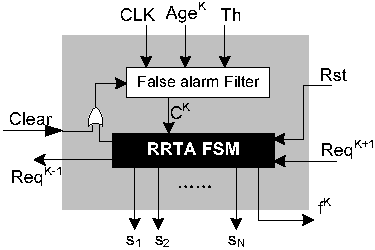
\includegraphics[width=0.36\textwidth]{fig2-20}%{agent.eps}
   \caption{Adaptation agent}\label{agent}
\end{figure}

Figure \ref{agent} shows the top view of an agent architecture. The agent can send a request $Req^{K-1}$ to an agent in the $(K-1)$st stage to enable forward adaptation for the $K$th stage logics, and can also receive $Req^{K+1}$ coming from an agent in the $(K+1)$st stage to enable forward adaptation for the $(K+1)$st stage logics. A failure signal ($f^K$) is asserted if an aging alarm still appears after the agent has traveled the all adaptation states.

Each agent consists of a RRTA unit and a False Alarm Filter; the RRTA is a finite state machine (FSM), and the filter is a counter. Signal $Age^K$, which is an aging alarm signal coming from an aging sensor, is cycle-updated. The adaptation process, however, should not be triggered at the same pace, otherwise it could incur useless adaptations due to the presence of \emph{false alarms}.

\subsubsection{False Alarm Filter}
The false alarms are caused by subtle dynamic variations \cite{degradation_05} such as power noise, temperature fluctuation. But aging can still be reliably detected even in the presence of these dynamic variations. The main reason is that the locations of aged paths generally won't change over time. This is very different from the power noise which mainly results from the time-varying current demand and exhibits much randomness in both spatial and temporary dimensions. Hence, the aging alarms traced back to the same spots are more "repetitive", by contrast to the more random dynamic variations. By exploiting the repetitiveness, we can filter the most, if not all, false alarms.

Identifying the ``repetitiveness" can be realized with a counter, which records the number of alarms in a specified span of time.  A confident aging alarm ($C^K$) is asserted only when corresponding counter reaches a threshold ($Th$) that has been calibrated according to some alarm statistics. To eliminate the aggregate effect of these false alarms, after each period of trial adaptation, the counter should be cleared.

Figure \ref{synadp} exemplifies the change of a filter counter over time. The normal perturbations (false alarms) have little chance to trigger adaptations; two adaption trials are conducted: the first fails, thus the counter still keeps growing after the invalid adaptation, while the second succeeds and the counter does not increase any more.

\begin{figure}[t]
\centering
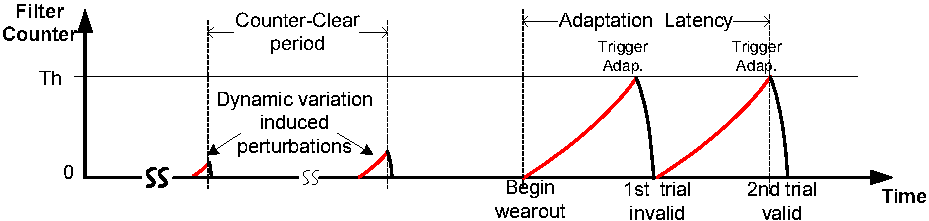
\includegraphics[width=0.8\textwidth]{fig2-21}%{cnt.eps}
   \caption{Example of filter counter change}\label{synadp}
\end{figure}


\subsubsection{Complexity Analysis and Two Critical Optimizations}\label{section_complexity} In Example \ref{rrtaexample}, for agent $A_K$ handling 7-bit clock-steering signals (3 bit for BAFFs and 4 bit for FAFFs), there are up to 22 ($2^3-1+2^4-1$) candidate states. Furthermore, each agent owns a private filter, which could incur non-negligible area overhead. Fortunately, with the following two optimizations the potential complexity can be decreased significantly.

Many adaptation state candidates can be removed with little loss of adaptability. The following shows how to use "logic cones" analysis to

1) remove those low-effective states for loose-couple logic cones, or

2) merge them for tight-couple logic cones.

\exmp Figure \ref{logiccone} exemplifies a stage of logic covered in two logic cones without overlap---loose-couple, referred to case (a) and with some overlap---tight-couple , referred to case (b). Suppose that flip-flop F1, F2, F3, and F4 are FAFFs and F5, F6 are BAFFs.

For case (a), the basic adaption states for F5 and F6 are \{01, 10, 11\}. Clearly, the state "11" is effective only in the case: (at least) one aged path in each logic cone causes aging alarm at the same time. Such ``coincidence", however, hardly happens; thus, we can safely remove the "11" from the adaptation state candidates. Similarly, the forward adaption states (for F1, F2, F3, F4) can be simplified from \{0001, 0010, $\ldots$, 1111\} to \{0001, 0010, 0100, 1000, 0011, 1100\}.

For case (b), the overlap can reduce some efficiency of such optimization. Removing state "11" for F5 and F6 may be problematic since an aging alarm could be raised at F5 and F6 simultaneously if aging happens in the overlap zone. For the same reason, the forward adaptation states should not be removed. However, since these two logic cones is tightly coupled, using 1-bit state for F5 and F6 should be reasonable. Then the backward adaptation states can be reduced from \{01, 10, 11\} to \{1\} . Similarly, the forward adaptation states can be simplified to \{001, 010, 100, 011, 110, 111\} (for F1, $<$F2,\,F3$>$, F4).


\begin{figure}[t]
\centering
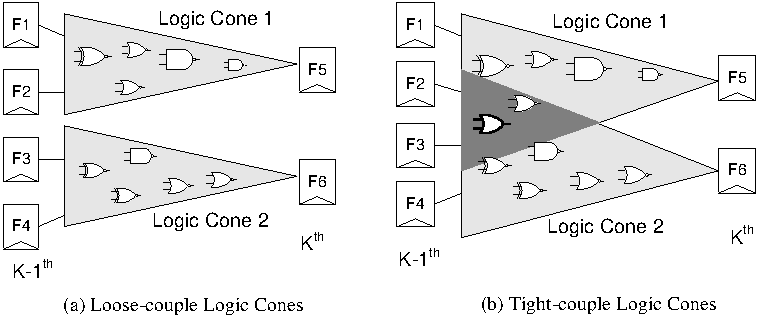
\includegraphics[width=0.7\textwidth]{fig2-22}%{logiccone2.eps}
   \caption{Logic cones}\label{logiccone}
\end{figure}

Each agent owning a private false-alarm filter is cost-inefficient, since such private filter is only necessary in such case: all the agents are active at the same time---that is a quite small probability event. Enabling filter sharing  can be readily implemented by appending selection-indicating bits $S$ to original filter. Figure \ref{agent_share} shows an example of two agents sharing one filter.

\begin{figure}[t]
\centering
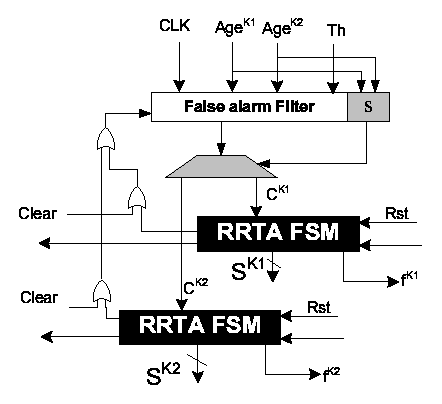
\includegraphics[width=0.45\textwidth]{fig2-23}%{agent_share.eps}
   \caption{Two agents share one false alarm filter}\label{agent_share}
\end{figure}


The above have described the individual agent design and functionality; the following will detail how to deploy the agents and corresponding sensors with respect to the correspondence of BAFFs, FAFFs, and UAFFs.

\subsubsection{Deploy Agents and Sensors}\label{deploy_agentsensor}
\begin{figure}[t]
\centering
\includegraphics[width=0.8\textwidth]{fig2-24}%{deploy2.eps}
   \caption{Deploying sensors and agents}\label{delpoy}
\end{figure}

Suppose that the $K$th stage with downstream flip-flops $$FF_{k}=\{f_1^{k}, \ldots,\; b_1^{k}, \ldots, b_s^{k}, \;u_1^{k}, \ldots, u_t^{k}, \;g_1^k, \ldots \}, $$ and upstream flip-flops $$FF_{k-1}=\{f_1^{k-1}, \ldots,  f_r^{k-1},\; b_1^{k-1}, \ldots, \;u_1^{k-1}, \ldots, \;g_1^{k-1}, \ldots \}.$$ Among these flip-flops, only $\{b_1^{k}$, $\ldots$, $b_s^{k}\}$ and $\{f_1^{k-1}$, $\ldots$, $f_r^{k-1}\}$ can contribute to the adaptation in the $K$th stage. We explain the policy of
deployment with the following example:

Figure \ref{delpoy} shows the $K$th stage's upstream and downstream flip-flops that can contribute to adaptation, and each sensor is assumed to handle eight signals at the most. Sensor $S_1$, $\ldots$, $S_n$ are assigned to $b_1$, $\ldots$, $b_s$, and $S_{n+1}$, $\ldots$, $S_m$ to $u_1,\ldots, u_t$. Furthermore, suppose that the upstream flip-flops can be divided into three loose-couple groups: $f_1,\ldots, f_p$ are relevant inputs to $b_9, \ldots, b_{16}$, $f_{p+1},\ldots, f_q$ to $b_{17}, \ldots, b_s$, and $f_{q+1},\ldots, f_r$ to $b_1, \ldots, b_8$. Three polices can be used to guide the deployment:

1) The agents are not required for the UAFFs, e.g. $u_1, \ldots, u_t$; but sensors is required,
i.e. $S_{n+1}$, $\ldots$, $S_m$.

2) The agents assigned to FAFFs, unlike that assigned to BAFFs, are triggered by the downstream agents, rather than by any sensors (so false alarm filters are not necessary for the FAFFs' agents).

3) The connecting relations between upstream agents and downstream agents is determined by the target circuit topology which can be obtained by conducting logic cones analysis (the ultimate goal of using logic cones analysis for ReviveNet is to extract all loose-couple logic cones, and merging all tight-coupling logic cones).

The number of required sensors $N_{sensor}$ for the $K$th stage is
\begin{equation}\label{numsensor}
N_{sensor}=\frac{s}{BW_{sensor}},
\end{equation}
where $BW_{sensor}$ denotes the maximum number of nodes that each sensor can handle.

The number of required agents $N_{agent}$ is
\begin{equation}\label{numagent}
N_{agent}=N_{agent}^{dn}+N_{agent}^{up},
\end{equation}
where $N_{agent}^{dn}$ denotes the number of downstream agents and $N_{agent}^{up}$ denotes that of upstream agents. Generally, each downstream agent is assigned a sensor and has the same bandwidth with the associated sensor, so \begin{equation}N_{agent}^{dn}=N_{sensor}\end{equation}. The number of upstream agents and its' bandwidth, however, is circuit topology-specific; thus the area of each upstream agents are not constant. For instance, the upstream A1, A2, and A3 in Figure \ref{delpoy} may handle different number of FAFFs (different bandwidth).

\begin{figure*}[t]
\centering
\includegraphics[width=0.95\textwidth]{fig2-25}%{agent_set.eps}
\vspace{-0.2cm}
   \caption{A group of synergistic agents for a n-stage pipeline}\label{sac}
\end{figure*}


Base on the above analysis, we present a typical organization of agents for a N-stage pipeline in Figure \ref{sac} (no filter sharing illustrated for simplicity), where $Age^K$ is a set of aging alarm signals from the $K^{th}$ stage and $S^K$ is a set of clock-steering signals to enable localized adaptations.

\subsection{Architecture Implementation}\label{imple_issue}

\subsubsection{Clock Generation and Overhead Analysis}\label{section_clcokgen}

ReviveNet needs two extra clocks, FCLK and BCLK, with intentional skew from CLK. These clocks can be generated by using a DLL(delay-locked loop). DLLs are widely used to reduce the clock skew across clock domains \cite{clock_01} \cite{DLL_00} \cite{DLL2_04}. The detailed design of a DLL is beyond the scope of this paper. A major concern is whether those PVT (process, voltage, and temperature) variations can spoil the intentional skew. Fortunately, many industry practices have shown that implementing clocks with only picoseconds of skew is very practical. For example, even in conventional tree-based clock networks across 500$mm^2$ processor die with frequency up to 2.5GHz , the unintended clock skew can be efficiently limited less than 10ps \cite{Itanium_clock05}. Thus, it can be extrapolated that for relatively spatial concentrated pipeline logics with less die area, the unintentional skew can be further optimized. In fact, even "10ps" is generally one order of magnitude smaller than the intentional skew. Moreover, the power consumption of a processor's DLLs, commonly, is less than 2\% \cite{clockpower_02}, and the hardware overhead is very limited. Hence, with the state-of-the-art clocking techniques, we believe that generating the adaptation clocks won't be a major obstacle.

In our scheme, we point out that although ReviveNet needs two extra clocks, our evaluation results show that on average the load of each of them is only about 20\% of CLK's. This is because only BAFFs and FAFFs need to be deployed with extra clocks, while the proportion of the two types of flip-flops takes only about 19\%. That means more than 80\% clock distributions are kept intact. This implies that 1) the clock power will not be tripled  but far less than that (section \ref{section_results}), and 2) the routing complexity will not be significantly increased. So, the overall design complexity should be in check.

\subsubsection{ReviveNet-supported Clock Gating}\label{section_clockgate}
\begin{figure}[t]
\centering
\includegraphics[width=0.7\textwidth]{fig2-26}%{clkgate.eps}
   \caption{ReviveNet-supported clock gating}\label{clkgate}
\end{figure}

Since aging adaptations usually are conducted on minority aging-prominent logics, so for the rest logics, It's better to keep the associated standby clocks off.

ReviveNet can readily support a high-efficient clock gating to further reduce the extra power consumed by the additional FCLK and BCLK. Figure \ref{clkgate} shows ReviveNet's clock network. The basic clock routing for CLK can be found in \cite{clockpower_02}. Usually, the pipeline will not suffer from aging in the early phase of lifetime, so FCLK and BCLK do not need to be enabled during that period. Two "root" clock gates, A and B, are employed to totally cut FLCK and BCLK off the DLL; thereby no power is consumed on the extra clock networks. If some parts of the pipeline need to be adapted, the corresponding root gate and branch gate can be switched on on-demand, while the unrelated clock branches are still kept off.

\subsubsection{Implication of Multi-cycle Paths}
Since a multi-cycle path usually consist more logic gates, the timing margin that a single-cycle path is able to share is likely to be inadequate. For example, suppose the cycle period is 1ns, for a 5-cycle path with fresh path delay 4.7ns. Then 10\% degradation yields 5.17ns ($4.7+4.7\times10\%$), which must violate the 5-cycle path timing requirement. But a single-cycle path can only contribute 0.075ns (1$\times$15\%/2) slack (suppose $TH$=0.15). Hence, although this slack, if exploited, can partially alleviate the aging delay, we had better not rely on single-cycle paths to salvage multi-cycle paths.

For multi-cycle paths, especially for "many-cycle" paths, we think a more effective way is to resort to some logic optimizations. For example, re-organize the 5-cycle paths into 6-cycle paths, to naturally gain more aging tolerability, though this approach usually needs to interact with some microarchitecture implications (which are supposed to beyond the scope of this paper).

\subsubsection{Impact of ReviveNet Wearout}\label{section_impactwearout}
Aging can indeed affect all logics on the chip, including aging sensors, adaptation agents, and even clocks networks.
	
Among them, the adaptation agents are relatively timing-non-critical; the latency of each adaptation, for example, increase from 1 cycle to 2 cycles should not be critical for an effective adaptation. This implies that, to protect these agents from the impact of aging, we can "over-design" the agents; that is to reserve conservative timing margins for these agents. For the clock networks, aging may results skew drift. Since skew-controlling actually is one of the primary objectives in many traditional clock optimizations, and we suppose that is beyond the scope of this paper. The sensor degradation, however, can impair the effectiveness of the proposed ReviveNet; after all, we cannot count on the adaptations triggered by unreliable sensors.
	
Fortunately, because the sensors' area and power overhead are small ($<$5\% and 1\%, respectively), so we can also over-design those sensors by using such as transistor-sizing techniques \cite{Temporal-Performance-Degradation-date06}. Usually, transistor-sizing impose about 9\% area overhead \cite{Temporal-Performance-Degradation-date06}, the overall extra overhead, therefore, should be very small.


\subsection {Modele Based Reliability Analysis}\label{section_model}

\subsubsection{Reliability Model}
Commonly, the reliability of semiconductor is modeled with Weibull distribution \cite{Handbook}. Given a circuit, the reliability at  time $t$ is given by
\begin{equation}\label{weibull}
  R(t)=\mbox{exp}[-(\frac{t}{\alpha})^\beta]
\end{equation}
where $\alpha$ is the characteristic time-to-failure and $\beta$ is the shape parameter \cite{Handbook}. The MTTF is calculated by
\begin{equation}
MTTF=\int^\infty_0 R(t)\,\mbox{d}t.
\end{equation}

Suppose that there are $n$ critical paths in the target circuits. The reliability of the $i$th path at time $t$ can be expressed as
\begin{equation}
  R_i(t)=P(T_i(t)<T)
\end{equation}

where, $T_i(t)$ denotes the delay of the $i$th path at time $t$; $T$ is the clock cycle period. Let's further assume that these paths are independent to each other, as Bowman et al. assumed in \cite{variation_jssc02}. Then, $R(t)$ can be put in another way:

\begin{equation}\label{anotherway}
  R(t)=\prod^n_{i=1} R_i(t)=\prod^n_{i=1} P(T_i(t)<T).
\end{equation}

Moreover, we treat each critical path as a "mini-component", then $R_i(t)$ can be expressed as
\begin{equation}
  R_i(t)=P(T_i(t)<T)=\mbox{exp}[-(\frac{t}{\alpha_i})^{\beta_i}],
\end{equation}
then we have
\begin{equation}
  R(t)=\prod^n_{i=1}
  \mbox{exp}[-(\frac{t}{\alpha_i})^{\beta_i}]=\mbox{exp}[-\sum^n_{i=1}(\frac{t}{\alpha_i})^{\beta_i}].
\end{equation}
The corresponding MTTF can be calculated by
\begin{equation}\label{mttf}
  MTTF=\int^{\infty}_{0} \mbox{exp}[-\sum^n_{i=1}(\frac{t}{\alpha_i})^{\beta_i}]\,\mbox{d}t.
\end{equation}

The above general analysis has not taken the effect of ReviveNet into account yet, and the following will involve it. When considering ReviveNet, the group of $\mathcal{R}=\{$$R_1(t)$, $R_2(t)$,$\ldots$, $R_n(t)\}$ can be divided into three groups according to the adaptability of each critical path:
\begin{itemize}
  \item Group 1: the set of critical paths in case 2) and 3) (Section 3.1) which can only be backward or forward adapted by $TH/2$;
  \item Group 2: the set of critical paths in case 1) which can not only be backward, but also forward adapted by $(TH/2+TH/2)=TH$;
  \item Group 3: the set of critical paths in case 4) which are unadaptable.
\end{itemize}

 Suppose that there are $l$ paths in Group 1, $m$ paths in Group 2, and the other $(n-l-m)$ in Group 3. Without  loss of generality, denote the first group as $\mathcal{R}_{u}=\{R_1(t), R_2(t),\ldots, R_l(t)\}$, the second group as $\mathcal{R}_{b}=\{R_{l+1}(t), \ldots, R_{l+m}(t)\}$, and the third group as $\mathcal{R}_{n}=\{R_{l+m+1}(t), \ldots, R_{n}(t)\}$. Then we have the ReviveNet-involved reliability term $\widetilde{R}_i(t)$, as follows:

\begin{equation}\label{new_term}
{\small
 \widetilde{R}_i(t)=\left\{
\begin{array}{ll}
P(T_i(t)<T+{TH}/{2}) & \mbox{if $i=1, 2, \ldots, l$,} \\
P(T_i(t)<T+ TH) & \mbox{if $i=l+1, \ldots, l+m$,} \\
P(T_i(t)<T) & \mbox{if $i=l+m+1, \ldots, n$.}
\end{array} \right.}
\end{equation}

The enhanced MTTF can be obtained:
\begin{equation}\label{mttfr}
MTTF_R = \int^\infty_0  \prod^n_{i=1} \widetilde{R}_i(t) \,\mbox{d}t.
\end{equation}

We define a relative MTTF improvement, $EX$ (short for "EXtension of lifetime"),  denoted by
\begin{equation}
  EX=\frac{MTTF_R}{MTTF}
\end{equation}
to evaluate the effect of ReviveNet.

To calculate $EX$ we have to figure out the relations: $\alpha_i=\alpha_i(T)$, and $\beta_i=\beta_i(T)$. Figure \ref{weibull} shows the qualitative relations; the following describes how to figure out the two relations.

In weibull distribution,
\begin{equation}\label{ab}
\beta=\frac{1.38}{\mbox{ln}(t_{50}/t_{16})},\;\mbox{ and }\; \alpha =
\frac{t_{50}}{ln(2)^{1/\beta}}\approx t_{63}
\end{equation}
where $t_x$ means the lifetime at the failure rate $x\%$ \cite{Handbook}, as shown in Figure \ref{weibull}. Intuitively, given a critical path, if more margin is reserved for it, then the wearout should be also postponed, as curve I and II show. ReviveNet can provide margin for some critical paths, thereby postponing the onset of wearout. In the following, relying on the assumption: the curve I and II are same in "shape", can greatly simplify the discussion, although the actual failure rate in the wearout region for I and II may slightly differ from each other.

Figure \ref{weibull} also reveals the effect of ReviveNet for a specific critical path can be reflected by the parameter $\alpha$ and $\beta$. Let $t_{50}= t_{16}+\Delta$, and commonly, $\Delta
\ll t_{16}$ then
\begin{equation}
  \beta=\frac{1.38}{\mbox{ln}(1+\Delta/t_{16})} \approx \frac{1.38}{\Delta/t_{16}}
\end{equation}

For the both curves, because $\Delta_I=\Delta_{II}$, so
\begin{equation}\label{frac}
\frac{\beta_I}{\beta_{II}}=
\frac{t_{16,I}}{t_{16,II}},\;\;\frac{\alpha_I}{\alpha_{II}}=\frac{t_{63,I}}{t_{63,II}}
\end{equation}


\begin{figure}[t]
\centering
\includegraphics[width=0.6\textwidth]{fig2-27}%{weibull2.eps}
\vspace{-0.2cm}
   \caption{Weibull failure rate in wearout period}\label{weibull}
\end{figure}

Furthermore, let
\begin{equation}\label{newab}
t_{16,II}=t_{16,I}+g(\delta) \mbox{ and }  t_{63,II}=t_{63,I}+g(\delta)
\end{equation}

where $g(\delta)$ denotes the lifetime extension contributed by tolerating $\delta$ aging delay; $\delta$ can be $0$, $TH/2$, or $TH$, determined by the specific adaptability of paths. Clearly, function $g(\delta)$ is highly dependent to specific aging mechanisms. Unfortunately, no such function proposed so far that can accurately reflect the performance degradation over time under a variety of aging mechanisms (some of them such as dielectric breakdown even have not been well-understood by the community \cite{Reliability_limits_IBM02}). In the following case study, we just use the relatively well-studied NBTI, one of the major reliability challenge, as target aging mechanism to evaluate the ReviveNet. We expect the physical community to contribute a much more versatile $g(\delta)$ in the near future.

Paul. et al. proposed a NBTI circuit delay model that capture the relation ship between the threshold voltage change and resultant delay degradation \cite{NBTI_Impact05}: the NBTI degradation is much fast at the early years, and then slowed down later, as the trend shown in Figure \ref{nbti}. Moreover, Figure \ref{nbti} also shows the relation between $\delta$ and $g$; we obtain $g(\delta)$ by regressing the results in \cite{wang2007impact}. More details are presented in Section 7.2.


\subsubsection{Implication of $TH$}\label{sec:th}
Eq. (\ref{new_term}) implies an essential tradeoff behind ReviveNet. Note that the critical paths in Group 3 is free from ReviveNet; only the Group 1 and Group 2 can contribute to the lifetime improvement. However, given a target circuits, the sizes of the three groups are depends on the $TH$: on one hand, larger $TH$ can result higher percentage of of UAFFs, and thereby more critical paths in Group 3, and thus leads to fewer adaptable critical paths; on the other, the larger $TH$ implies that more aggressive tolerability to aging delay on those adaptable critical paths. Hence, given a circuit, there should be an optimum $TH$ that can maximize the $EX$.


\begin{figure}[t]
\centering
\includegraphics[width=0.45\textwidth]{fig2-28}%{nbti2.eps}
\vspace{-0.3cm}
   \caption{NBTI degradation}\label{nbti}
\end{figure}

\subsection{Case Study and Discussion}\label{section_casestudy}
\subsubsection{Experiment Setups}
We took a fully pipelined FPU \cite{OpenSPARC_06} as our target circuit which implements the SPARC V9 floating-point instructions and supports all IEEE 754 floating-point data types. The FPU comprises three independent pipelines: Multiplier pipeline (MUL), Adder pipeline (ADD) and Divider pipeline (DIV). In this paper, we used the largest MUL, which takes up to 50\% area of the FPU, as the target pipeline. More design details can be found in \cite{OpenSPARC_06}.

The FPU was synthesized using Design Compiler with UMC
0.18um technology. We set the performance as the synthesizing priority to smooth the distribution
of path delay as much as possible. Then, the path delay was analyzed with PrimeTime.

First, we identify the adaptability of each pipeline flip-flop, based on the STA results. Then, the
deployment of sensors and agents can be determined as follows: for each flip-flops $i$, find the
upstream flip-flops that in the same logic cone; this can be done by matching the start points of
paths ended with the flip-flop $i$. The number of required sensors and agents can be figured out by
using Eq.(\ref{numsensor}) and Eq.(\ref{numagent}).
Then, we evaluate the MTTF improvement ($EX$) by using the proposed reliability model.
Finally, we present the overhead in terms of area, power, and performance.

\subsubsection{Results and Discussions}\label{section_results}

\begin{figure*}[t]
\centering \subfigure[\small{Skew variation: 1\%}]
%{\includegraphics[width=0.34\textwidth]{EX2_1percent.eps}} \hspace{-0.5cm}
{\includegraphics[width=0.34\textwidth]{fig2-29a}} \hspace{-0.4cm}
\subfigure[\small{Skew variation: 3\%}]
%{\includegraphics[width=0.34\textwidth]{EX2_3percent.eps}}\hspace{-0.5cm}
{\includegraphics[width=0.34\textwidth]{fig2-29b}} \hspace{-0.4cm}
\subfigure[\small{Skew variation: 5\%}]
%{\includegraphics[width=0.34\textwidth]{EX2_5percent.eps}} \vspace{-0.2cm}
{\includegraphics[width=0.34\textwidth]{fig2-29c}} \hspace{-0.4cm}
\vspace{-0.2cm}
\caption{MTTF improvement at different $TH$ and clock skew variations}\label{ex}
\end{figure*}

\textbf{Lifetime Improvement Analysis:} We conduct the lifetime evaluation based on the 65nm technology (the STA results actually are based
on a 180nm technology due to lack of 65nm compiler libraries. To match the following analysis, we
scale the STA results to 65nm based on scaling theory \cite{JMRabaey}). The NBTI degradation
results are from \cite{wang2007impact}. The lifetime is studied at different configurations:
without ReviveNet, and with ReviveNet, at $TH$=5\% (of the delay of the most critical path), 10\%,
15\%, 20\%, 25\%, 30\%, respectively. The necessary $g(\delta)$ at these $TH$ is as follows:
\begin{equation}\label{reg}{\small
\begin{array}{ll}
g(0.05)=876 \mbox{(hours)}; &g(0.1)=8,760 \mbox{(hours)};\\
g(0.15)=21,900 \mbox{(hours)};& g(0.2)=43,800 \mbox{(hours)};\\
g(0.25)=87,600 \mbox{(hours)};& g(0.3)=131,400 \mbox{(hours)}.
\end{array}}
\end{equation}

For example, $g(0.05)=876$ (hours) means that the 5\% tolerability to delay degradation can
translate to 876 hours lifetime extension. The above results faithfully reflect that NBTI
degradation which is much faster at the early years and slowed down over time.

Next, the weibull parameter $\alpha$ and $\beta$ is calculated as follows: we use empirical data:
$t_{16}=35,040$hours (4 years) and $t_{63}=39,420$hours (4.5 year) (thus $\Delta=4380$ hours).
Then, from Eq.(\ref{ab}), we have the original $\alpha$ and $\beta$ for a critical path is
$\alpha=39,420 \mbox{ (hours)}, \beta=11.04$.
Then, combined Eq.(\ref{reg}) with Eq.(\ref{newab}) and then put it into Eq.(\ref{frac}), the new
$\alpha$ and $\beta$ at different $TH$ can be obtained. When calculating MTTF, we
assume that the critical paths with the same adaptability have the same $\alpha$ and $\beta$.

Finally, base on the STA results, the three path groups $\mathcal{R}_u$, $\mathcal{R}_b$, and
$\mathcal{R}_n$ at different $TH$ configurations can be determined, respectively.

With the above preparation, the original and improved MTTF can be calculated with Eq.(\ref{mttf})
and Eq.(\ref{mttfr}); Figure \ref{ex} shows the detailed results that offer a significant insight: larger $TH$ does not necessarily results higher improvement in lifetime reliability.
The underling reason is on one hand larger $TH$ can facilitate more aggressive timing stealing, thereby
improving more reliability for adaptable paths; on the other, larger $TH$ will definitely results
more UAFFs and thereby more unadaptable paths. In other words, the overall MTTF is determined not
only the reliability benefit of individual path, but also the population of paths governed by
ReviveNet. At the optimum configuration, $TH$=20\%, MTTF can be improved by 48.7\%.

\textbf{Impact of Clock Skew Variation:} The effectiveness of ReviveNet, as concerned in Section \ref{section_clcokgen}, is also impacted by the variation in clock skew (measured by $skew/cycle\_period$ in this paper). The impact actually results in corresponding variation in ``effective" $TH$. We find that the degradation can only be marginally impacted if the adaptation clocks are kept beyond a large interval, say, $TH>0.2$. Specifically, Figure \ref{ex}(a), (b), and (c) show the $EX$ variation under different clock skew variations: 1\%, 3\%, and 5\%, respectively. Two trends can be clearly identified: i) the degradation in effectiveness  reduces with  $TH$ increasing, and ii) the larger clock skew variation results in more variation in MTTF improvement. Hence, the worst-case efficacy under overly ``weak" adaptation intensity, i.e. $TH<0.1$, can be significantly reduced under 3\% skew variation, and even totally diminished under 5\% skew variation, as shown in Figure \ref{ex}(b) and (c). However, the optimal design point is around $TH=0.2$ where the impact of clock skew is marginal.

In addition, it is practical to keep the clock skew below 3\% by using the state-of-the-art clocking techniques (for example, 10ps skew variation for 2.5GHz Itanium processor \cite{Itanium_clock05}). This can further justify the effectiveness of ReviveNet.



\textbf{Overhead Analysis:} We evaluate ReviveNet's overhead from three aspects: silicon area, power, and performance. The
overhead largely depends on the parameter $TH$ (section 7.2).

\smallskip
\noindent{\bf 1. Area Overhead.}

{\bf Sensor Configuration:} The number of sensors for each stage depends on specific sensor design
\cite{agarwal2007circuit}\cite{SVFD_09};

we take the configuration of one sensor handles eight signals.



{\bf Agent Configuration:} Agents are configured as follows: 6-bit False Alarm Filter which can
filter as much as 64 false alarms during one adaptation period. We study the area overhead with
different degrees of Filter sharing: no sharing, two agents sharing one filter, four agents sharing
one filter, and eight agents sharing one filter.



The sensor and agents are insert into the original MUL netlist, and re-synthesized using the same
technology. Figure \ref{totalarea} shows the overall area overhead under different configurations. Generally, the area overhead is small: only 9.5\% at the recommended $TH$=0.2.

\begin{figure}[t]
\centering
\includegraphics[width=0.55\textwidth]{fig2-30}%{areaoverhead.eps}
\vspace{-0.3cm}
   \caption{Area overhead with different sharing configurations}\label{totalarea}
\end{figure}


\smallskip \noindent{\bf 2. Power Overhead.}

Power overhead mainly comes from ReviveNet logics (sensors and agents) and extra clock networks.
That is
$$P_{overhead}=P_{logic}+P_{clk}=(P_{sensor}+P_{agent})+P_{clk}.$$ The following results show that
$P_{logic}$ is negligible, and the major power overhead results from $P_{clk}$.

{\bf 1) Logic Power.} We use PrimePower to evaluate $P_{logic}$. Evaluation results
show that even in the worst case\,---\,each sensor raises an aging alarm in every cycle\,---\,the
power overhead caused by the sensors and agents is negligible. Figure \ref{logicpower} shows that a
typical logic power overhead ($TH=0.2$) is less than 5\%.


{\bf 2) Clock Power.} The worst case overhead of clock power, $P_{clk}$, is more significant than that
of logics. In ReviveNet, the clock power can be calculated as
$$P_{clkall}=P_{pipeffs} + P_{DLL} + P_{buf} + P_{wire}+ P_{mux} \, \mbox{\cite{clockpower_02}} $$ where
$P_{pipeffs}$ and $P_{DLL}$ is the power consumed by pipeline flip-flops and DLL, and $P_{buf}$,
$P_{wire}$, and $P_{mux}$, are power consumed by  clock buffers (drivers), clock wires, and clock
multiplexers, respectively. $P_{pipeffs}$ and $P_{DLL}$ stay unchanged because little modifications
are made to them. The clock buffers which take the most proportion, 56\%,  in the original
pipelines, increase by 32\% to support FCLK and BCLK networks (the increase in buffers is
proportion to the increase in clock load). $P_{wire}$ almost triples, but it takes only about 10\%
in original pipelines. Compared with the other proportions, $P_{mux}$ is ignorable. Overall, the
clock power increases by 38\%.

The previous study \cite{clockpower_02} shows generally for a pipelined processor,
the clock power is about the 30$\backsim$40\% (denoted by $\eta$) of the total power,
so this increase contribute to the overall power overhead is calculate by
$$[(1-\eta) + \eta \times (1+38\%)] - 100\%.$$
Since $\eta$ is about 30$\backsim$40\%, the overall overhead should be between 11.4$\backsim$15.2\%.

Note that this overall power overhead is in the \emph{Worst Case}---all the drivers of FCLK and BCLK
are turned on. However, little power overhead is imposed in the early period of lifetime, because
few of the extra logics and clock networks need to be turned on due to  little appreciable aging
delay. Moreover, we believe with ReviveNet-supported clock gating, the overall power
overhead can be significantly reduced even after the onset of wearout.



\smallskip \noindent{\bf 3. Performance Overhead.}

ReviveNet needs some sensors. From circuit design perspective, these sensors can cause some
capacitance load to the target pipelines. This concern, however, will not be substantial because
the performance penalty imposed by such capacitance load is less than 1\%
\cite{agarwal2007circuit}\cite{SVFD_09}.


\begin{figure}[t]
\centering
\includegraphics[width=0.5\textwidth]{fig2-31}%{poweroverhead_workmode.eps}
\vspace{-0.3cm}
   \caption{Power overhead of sensors and agents in working mode}\label{logicpower}
\end{figure}

ReviveNet improves the lifetime reliability only by tolerating the aging delay, which may not be
comprehensively enough. In addition, ReviveNet does not suppose to handle some "abrupt" wearout
which in reality is possible due to some mechanical stress induced failures.
In addition, ReviveNet is not designed for coping with all corner cases, but for average case;
in other words, ReviveNet is statistically effective, rather than deterministic.

\section{Summary}
The proposed ReviveNet architecture, without compromising with the nominal architectural
performance, can efficiently hide the aging induced delay, thereby improving the lifetime
reliability. The weakest links of lifetime can be locally and efficiently remedied by enabling a
path-grained adaptation mechanism; ReviveNet employs a group of collaborative cost-efficient agents
to achieve this purpose. A new reliability model is also proposed to quantitatively evaluate the
effect of ReviveNet. Evaluation results based on a case study show that the ReviveNet can improve
the MTTF by 48.7\%, at the expense of about 9.5\% area overhead, and about 4.9\% power increase during aging-free period.

\bibliographystyle{plain}
\bibliography{refs}

%%%%%%%%%%%%%%%%%%%%% chapter.tex %%%%%%%%%%%%%%%%%%%%%%%%%%%%%%%%%
%
% Chapter 3
%
% Use this file as a template for your own input.
%
%%%%%%%%%%%%%%%%%%%%%%%% Springer-Verlag %%%%%%%%%%%%%%%%%%%%%%%%%%
%\motto{Use the template \emph{chapter.tex} to style the various elements of your chapter content.}
\chapter{Fault-Tolerant General Purposed Processors}


\abstract{In field degradation of manycore processors poses a grand challenge to core management, largely because the degradation is hard to quantify. We propose a novel core-level degradation quantification scheme, CoreRank, to facilitate the management. We first develop a new degradation metric, called “healthy condition”, to capture the implication of performance degradation of a core with specific degraded components. Then, we propose a performance sampling scheme by using micro-operation streams, called snippet, to statistically quantify cores’ healthy condition.We find that similar snippets exhibit stable performance distribution, which makes them ideal micro-benchmarks to testify the core-level healthy conditions. We develop a hardware-implemented version of CoreRank based on bloom filter and hash table. Unlike the traditional “faulty” or “fault-free” judgement, CoreRank provides a key facility to make better use of those imperfect cores that suffered from various progressive aging mechanisms such as NBTI, HCI. Experimental results show that CoreRank successfully hides significant performance degradation of a defective manycore processor in which even more than half of the cores are salvaged from various defects.}

\section{Challenges of Fault-Tolerant Processor Design}

\subsection{Processor Vulnerability Characterizing}
With the continuous decrease of CMOS feature size and threshold voltage, microprocessors are expected to see increasing failure rates due to intermittent faults, in company with soft errors and hard faults \cite{mcpherson2006reliability} \cite{constantinescu2003trends} \cite{karnik2004characterization}. Intermittent faults are hardware errors which occur frequently and irregularly for a period of time, commonly due to manufacturing residuals or process variation, combined with voltage and temperature fluctuations \cite{constantinescu2002impact} \cite{wells2008adapting}. Soft errors, namely transient faults, are caused by energetic particles such as alpha particles from packaging material and neutrons from the atmosphere. Hard faults reflect irreversible physical changes, mainly caused by manufacturing defects, such as contaminations in silicon devices or wear-out of materials. Conventionally, soft errors and hard faults have been considered as the major factor of program failures, and the effects of these faults have been extensively analyzed \cite{shivakumar2002modeling} \cite{srinivasan2004impact}. Nevertheless, field collected data and failure analysis show that intermittent faults also become a major source of failures in new-generation microprocessors \cite{constantinescu2008intermittent}. Without protection techniques, the microprocessor failure rates due to these faults will greatly increase with the exponential growth in the number of transistors.

To improve system reliability, prior work has proposed a variety of techniques to deal with these faults from circuit level to architecture level. Optimal protection techniques should meet a predefined reliability budget while with minimal performance, area, and energy penalties. As the number of ways that different faults manifest are likely to rise, leading to a consequential increase in the complexity and overhead of the techniques to tolerate them. Traditional protection techniques, for example, dual or triple modular redundancy results in at least 100\% hardware and energy overhead \cite{Slegel1999IBM} \cite{wood1999data}. Solutions such as full redundant multithreading (RMT) and various partial redundancy schemes based on RMT also lead to about 30\% performance degradation \cite{mukherjee2002detailed} \cite{reinhardt2000transient} \cite{parashar2006slick} \cite{shyam2006ultra}. In a recent workshop, an industry panel converged on a 10\% area overhead target to handle all sources of chip errors as a guide for microprocessor designers \cite{li2008understanding}. Therefore, designers should evaluate the pros and cons of different protection techniques. Heavyweight protection techniques (such as strict hardware duplication) can ensure system reliability but incur unnecessary overheads, while lightweight protection (such as partial software redundancy) techniques can reduce the protection overheads but may be hard to satisfy the desired reliability goal.

Researchers have utilized several metrics to guide microprocessor reliability design. Two most widely used metrics are mean time to failure (MTTF) and failures in time (FIT). MTTF and FIT are used as metrics to describe component reliability, but are incapable of explicitly characterizing the inherent masking effect of hardware structures to a fault and the utilization of different structures. Recently, researchers have proposed several architecture level metrics to characterize the vulnerability of microprocessor structures to soft errors and hard faults. Mukherjee et al. \cite{mukherjee2003systematic} propose architecture vulnerability factor (AVF) to describe the probability that a soft error in a structure leads to an external visible error. Sridharan et al. \cite{sridharan2009eliminating} \cite{sridharan2010using} propose two metrics program vulnerability factor (PVF) and hardware vulnerability factor (HVF) to characterize the masking effect of soft errors at architecture level and microarchitecture level, respectively. Bower et al. \cite{bower2006applying} introduce hard-fault architectural vulnerability factor (H-AVF) to help designers to compare various hard-fault tolerance methods. Since intermittent faults are very different from soft errors and hard faults, existing evaluation metrics can not accurately reflect the vulnerability of microprocessor structures to intermittent faults. With intermittent faults gradually becoming a major source of failures, a simple and quantitative metric is needed to guide reliable design for microprocessors. Having such a metric will help designers analyze which part of a microprocessor is more vulnerable to intermittent faults, and then select optimal protection techniques at an early design stage. However, characterizing the vulnerability to intermittent faults is far from mature.

In the first part of this chapter, we propose a metric intermittent vulnerability factor (IVF) to represent the probability that an intermittent fault in a structure will manifest itself in an observable program output.We analyze IVFs for two representative microprocessor structures: reorder buffer and register file.We then propose several IVF computation algorithms considering three intermittent fault models: intermittent stuck-at-1 and stuck-at-0 fault model, intermittent open and short fault model, and intermittent timing fault model. We exploit a cycle-accurate simulator Sim-Alpha to implement the proposed IVF computation algorithms and use SPEC CPU2000 integer benchmark suite as the workload.

\subsection{Sick Processor Management}
The growing integration density of transistors has been escorted by progressive semiconductor technologies for the past three decades. Unsurprisingly, the scale and complexity of modern microprocessors have reached a unprecedented level, and 1000-core processor will not be a buzz word but reality \cite{thousandcore}.  Unfortunately, we still face grand challenges to drive such powerful processor with a sea of computing cores to work efficiently.

One of the looming challenges is core management, which directly determines the harvestable performance of the powerful hardware substrate.  This challenge in essence comes from the core-to-core heterogeneity, either \emph{intentional} due to architectural innovations such as "bigLITTLE" architectures \cite{biglittle}, or \emph{unintentional} due to process variation \cite{variation_jssc02} \cite{ParameterVariations_DAC03}, aging \cite{ImpactTechnologyScaling_04} \cite{aging_iedm} \cite{degradation_05} \cite{ReviveNet}, and core salvaging \cite{redundancy_iccd} \cite{WearoutRecovery_08}, i.e. decoupling some faulty microarchitectural components for reliability reasons. Such core-to-core heterogeneity results in functionally equivalent cores with different performance levels. Intel and ARM demonstrated adaptive RISC core designs to tolerate such dynamic variations, at the expense of performance degradation \cite{adaptive-core} \cite{arm-timing-error}. In the near future, we believe that the core-level unintentional heterogeneity would be more significant, given the faulty components and aging effects would be more prevalent and prominent in smaller technology nodes \cite{degradation_05}.  We call such aging-induced performance degradation as "Sick Silicon" problem. Therefore, \emph{instead of simply ruling out those cores salvaged from various defects, we should try to hide the imperfections.}

An obvious solution to this problem is always prioritizing the cores with the least "degradation". However, we find that it's not that intuitively simple to  quantify the degradation. First, the performance degradation depends on both applications and defect degrees, as Figure \ref{degrade} shows. The results show the performance responses of cores under various types of degradations. The cores are salvaged from instruction window defects, or L1 instruction/data cache defects, or L2 cache defects, respectively \cite{salvaging}. For simplicity, we don't show the more complicated compound defects. The degradation degree of "0" indicates defect-free, and 1/2  indicate a half resource unavailable, and so on. The results show that  performance response not only depends on degradation degrees, but also exhibits to be highly application-specific. For example, the \texttt{gobmk} in the Figure \ref{degrade} (UL) shows to be very resilient to the instruction window degradation, but, by contrast, the \texttt{leslie3d} and \texttt{GemsFDTD} are very sensitive to it. Such complexity is never unique for instruction window only, but also to other resources, as exemplified in the other three sub-figures. Hence, even though the defect and associate defect degree are accessible to operating system (OS), we still have no ways to figure out how much performance impact such degradation to the running applications. Second, the performance degradation of different phases can also change significantly, even on the same core. Hence, the degradation measured in coarse-grained application may underestimate the impact of core-to-core heterogeneity. For example, assume an application is divided into two phases, Phase 1 and Phase 2. The execution time of the two phases on Core A is 100ms and 200ms, denoted by

\begin{equation}\nonumber
    T(\text{\footnotesize{Core A, Phase 1}})=100ms, T(\text{\footnotesize{Core A, Phase 2}})=200ms. 
\end{equation}
Suppose that the execution time of the same application on Core B, which is salvaged from a different defect component,   is

\begin{equation}\nonumber
    T(\text{\footnotesize{Core B, Phase 1}})=200ms, T(\text{\footnotesize{Core B, Phase 2}})=100ms. 
\end{equation}
Clearly, the performance of Core A and Core B have no difference for this application because both cores take  the same time, i.e. 300ms,  to finish. An obvious defect-hiding optimization is to schedule Phase 1 to Core A, and Phase 2 to Core B, the execution time can be reduced to 200ms. However, this opportunity is invisible if oblivious to the phase-specific degradation to heterogeneous cores.

In view of the above two observations, we claim that to maximally hide the defect-induced performance degradation, the prerequisite is to know how much degradation the phases of running application to specific cores. We use the term "healthy condition" to capture the function that a core performance is both phase- and defect-specific, denoted by $H(core_i|phase_j)$. Unfortunately, it is challenging to dynamically figure out $H(core_i|phase_j)$ because of the stochastic characteristics of application performance, as elaborated in Section 2. Simply put, how can we know which core can deliver the best performance for the coming phase of an in-flight application?

\begin{figure}[t]
    \centering
    \includegraphics[width=0.75\textwidth]{IPCDegradation.eps}\\
    \caption{Performance degradation  vs. defect degrees of inst. window  (UL), L1 inst. cache (UR), L1 data cache(LL), L2 cache(LR)}
    \label{degrade}
\end{figure}

In the second part of this chapter, we propose a statistical core ranking mechanism, called "CoreRank", to dynamically quantify individual core's healthy condition. CoreRank indicates the OS to avoid the unhealthy cores as much as possible, and always prioritize the healthier ones. Since the healthy condition can be reflected by the performance responses, and quantifying healthy condition is not very timing critical,  we can sample sufficient runtime performance statistics to infer each core's healthy condition. These statistics can be obtained by performance counters. Note that the inference is not one-time procedure, but in a progressive way. CoreRank never finishes its mission even all cores are testified, but periodically invoked to keep tracking them over the lifetime to capture the in field degradations. CoreRank establishes two principles: First, unlike distinguishing between faulty and fault-free cores in the realm of design for reliability, healthy condition should be a "conditional" probability, given a core's healthy condition is highly workload dependent. For example, a core with a faulty branch predictor shows to be healthier when comes to  branch-non-intensive applications than to branch-intensive ones. The application-dependent characteristic implies that the healthy condition should be conditionally defined. Second, CoreRank should not be tied with any specific applications. Quantifying healthy condition towards different applications is less useful because 1) the applications can be extremely diversified, and 2) the impact of inter-application interference on a highly parallel architecture is sporadic and hard to quantify.  CoreRank quantifies healthy condition towards  more specific phase representations, called "snippets", which are dynamic micro-operation streams and oblivious to all of the software level interferences. The snippet can be readily characterized by build-in performance counters, without any instrumentation to running workloads.

\section{Processor Vulnerability Evaluation}
\subsection{Vulnerability Analysis Methods}
Our work is related to several recent researches on characterizing the vulnerability of microprocessor structures to soft errors and hard faults. Architecture vulnerability factor (AVF) is a widely used metric to characterize the masking effect of soft errors both from microarchitecture level and architecture level \cite{mukherjee2003systematic},\cite{biswas2005computing} \cite{fu2006sim}. A structure’s AVF is the probability that a soft error in it causes an external visible error. The AVF can be calculated as the average-over-time percent of architecturally correct execution (ACE) bits in a structure. The ACE bits are those if been changed will affect the final output of a program, and on the contrary, un-ACE bits are those if been changed will not propagate to program output. For example, the AVF of a storage cell is the percentage of cycles the cell contains ACE bits; the AVF of a function unit is the percentage of cycles the unit processes ACE bits or ACE instructions. ACE bit analysis is carried out with a performance level simulator during program execution. Equation \ref{eq:avf} describes how to compute a structure’s AVF through ACE bit analysis, where $B$ is the total bits in a hardware structure, $T$ is the execution cycles of a program, and $N_{ACE}^{t}$ is the number of ACE bits in the structure at a specific cycle $t$.

\begin{equation} \label{eq:avf}
    AVF=\frac{\sum_{t=0}^{T}N_{ACE}^{t}}{B \times T}
\end{equation}


Another method to compute AVF is through statistical fault injection \cite{wang2004characterizing} \cite{touloupis2007study}. Fault injection experiments are performed on a register transfer level (RTL) model of microprocessors. After injecting a fault, the architecture state of the fault injected simulator will be compared with a golden model to determine whether the injected fault results in an external error. After a huge number of fault injections, the percentage of faults leading to external errors is taken as AVF. Statistical fault injection is able to simulate any execution path and allows for high accuracy estimation. Most recently, Walcott et al. \cite{walcott2007dynamic} use linear regression to identify the correlation between AVF and several key performance metrics (such as instructions per cycle and reorder buffer occupancy), and then use the predictive model to compute AVF dynamically during program execution. Duan et al. \cite{duan2009versatile} propose an alternative prediction method to compute AVF across different workloads and microprocessor configurations using boosted regression trees and patient rule induction method.

Prior works also demonstrate that AVF varies significantly and highly depends on microarchitecture structures and architecture programs \cite{pan2009online}. In order to characterize the vulnerability of a program independent of microarchitecture structures, Sridharan et al. \cite{sridharan2009eliminating} propose PVF to evaluate the masking effect of soft errors at architecture level. They use A-bits (like ACE bits) and architecture resources (the structures which can be seen from the perspective of programmers, such as register file and arithmetic logic unit) to compute PVF. Equation \ref{eq:pvf} is utilized to compute an architecture resource’s PVF where $B$ represents the total bits in the architecture resource, $I$ represents the total number of instructions in the program and $N_{A-bit}^{i}$ represents the number of A-bits in instruction $i$. PVF can be used to quantitatively estimate the masking effect of a program to soft errors and to express the behavior of AVF when executing a program. There are also several practical uses of PVF, such as choosing proper algorithms and compiler optimizations to reduce the vulnerability of a program to soft errors. Recently, Sridharan et al. \cite{sridharan2010using} propose another metric HVF to analyze the vulnerability to soft errors only from microarchitecture level.

\begin{equation} \label{eq:pvf}
    PVF=\frac{\sum_{i=0}^{I}N_{A-bit}^{i}}{B \times I}
\end{equation}

AVF, PVF, and HVF, all of them are focusing on the masking effect of soft errors. Bower et al. \cite{bower2006applying} propose a metric named H-AVF for hard faults. H-AVF allows designers to compare alternative hard-fault tolerance schemes. For a given program, a structure’s H-AVF can be computed as Equation \ref{eq:havf} where $N_{i}$ represents the total number of instructions in the program, $N_{f}$ represents the total number of fault sites in the structure, and $inst_{error}$ represents the number of instructions that will be corrupted due to hard faults. The purpose of H-AVF is to evaluate whether a particular sub-structure in microprocessors will benefit from hardening. It can also be used to compare hard-fault tolerance designs thus to provide a quantitative basis for comparison of alternative designs. Besides, Pellegrini et al. \cite{pellegrini2008crashtest} propose a resiliency analysis system called CrashTest. CrashTest is capable of orchestrating and performing a comprehensive design resiliency analysis by examining how the design reacts to faults during program execution. This method mainly considers the impact of hard faults and soft errors on program execution.

\begin{equation} \label{eq:havf}
    H-AVF=\frac{1}{N_{i}} \times \frac{1}{N_{f}} \times \sum_{\forall fault}^{}\sum_{\forall inst}^{}inst_{error}
\end{equation}

Unlike soft errors and hard faults, intermittent faults have many uncertain causes and their behaviors vary significantly. However, the vulnerability of microprocessor structures to intermittent faults is rarely considered. In this paper, we propose a metric IVF to characterize the vulnerability of microprocessor structures to intermittent faults. We compute IVFs for different microprocessor structures considering three intermittent fault models: intermittent stuck-at-1 and stuck-at-0 faults, intermittent open and short faults, and intermittent timing faults.

\subsection{Intermittent Fault Oriented Analysis}
This section first describes our IVF evaluation algorithms for different intermittent fault models, and then presents the equations for IVF computation. A structure’s IVF is defined as the probability that an intermittent fault in the structure leads to an external visible error. The higher IVF, the more a structure is vulnerable to intermittent faults. In modern microprocessors, reorder buffer and register file are two of the most important hardware structures.

\begin{figure}[t]
    \centering
    \includegraphics[width=0.75\textwidth]{IVF-fig4}\\
    \caption{(a) Schematic diagram of a baseline microprocessor. The two gray units are the structures under analyzing; (b) Reorder buffer entry \cite{shen2013modern}}
    \label{fig:baseline-processor}
\end{figure}


Fig. \ref{fig:baseline-processor}(a) shows a baseline pipeline used in this work. Reorder buffer is used for out-of-order instruction execution, which allows instructions to be committed in-order. It keeps the information of in-flight instructions and allows for precise exceptions and easy rollback for control of target address mispredictions. The entry in reorder buffer is allocated in a round-robin order. Fig. \ref{fig:baseline-processor}(b) further shows typical fields contained in an entry of reorder buffer \cite{shen2013modern}. These fields have different functions. The busy flag, issued flag, finished flag, speculative flag, and valid flag are control signals, while $PC$ denotes the address of the current instruction, and rename register shows the renamed register for the destination register of an instruction. For register file, it is an array of processor registers and will be used to provide operation data during program execution. Each register in it contains 64 bits. If any of these two structures is affected by an intermittent fault, the probability resulting in a visible error is very high.We compute IVFs for these two representative structures in this work.

Before IVF computation, the following two questions should be carefully answered.

1) How to determine whether an intermittent fault affects program execution?

2) In order to describe intermittent faults, how to set these three key parameters: burst length, active time, and inactive time appropriately?

For the first question, to evaluate the impact of an intermittent fault on program execution, we need to determine whether the fault propagates to a storage cell and changes ACE bits during its lifetime. For intermittent stuck-at faults, as they only affect a single location, we should check whether the affected location contains an ACE bit, and then analyze whether the ACE bit is upset during the fault’s active time. Only the case when the affected location contains an ACE bit and the ACE bit is changed will affect program execution. For intermittent open and short faults, they may corrupt two adjacent bit lines. When such a fault occurs, we need to determine whether the fault propagates to a storage cell and change ACE bits. While for intermittent timing faults, they may cause timing violations and affect write operations. Only when an intermittent timing fault has been captured by a storage structure and changes ACE bits, it will affect program execution.

\begin{figure}[t]
    \centering
    \includegraphics[width=0.75\textwidth]{IVF-fig5}\\
    \caption{Example of intermittent timing faults caused by voltage emergencies.}
    \label{fig:timing-faults}
\end{figure}

For the second question, the parameters of an intermittent fault should follow the characteristics of an actual fault. As intermittent faults may be caused by different factors, the duration of intermittent faults could vary across a wide range of timescale. To set appropriate values for these key parameters, we analyze one kind of intermittent timing faults caused by significant voltage variation. The situation when supply voltage variation across a allowed voltage threshold is called a voltage emergency \cite{joseph2003control}. Voltage emergencies will lead to timing violations by slowing logic circuits. Fig. \ref{fig:timing-faults} shows an example of intermittent timing faults caused by voltage emergencies. As can be seen, intermittent timing faults caused by voltage variations usually last on the order of several to tens of nanoseconds. Prior works also show the similar duration of an intermittent fault \cite{smolens2007detecting} \cite{gracia2008analysis} \cite{stathis2001physical}. According to the observation, we set the burst length of an intermittent fault in the range of 5 cycles to 30 cycles in our experiments. Both active time and inactive time are set to 2 cycles. The number of activations will be changed according to burst length, but the 50\% duty cycle is kept constant. For an instance, if burst length is 30-cycle, the number of activations is 8. Besides, as the appearance time of intermittent faults cannot be predicted, their start time are randomly generated during program execution.

Based on the above analysis, the first step for IVF computing is to determine ACE bits in a structure during program execution; the second step is to check whether ACE bits are changed when an intermittent fault occurs. As reorder buffer is used to support out-of-order instruction execution, we analyze ACE bits in it by monitoring instructions when these instructions go through all stages of the pipeline. Meanwhile, register file is used to store and provide operation data for in-flight instructions, we analyze ACE bits in it based on its related operations, such as read, write, and evict. Following we present IVF computation algorithms for intermittent stuck-at faults, intermittent open and short faults, and intermittent timing faults, respectively.

\subsubsection{Intermittent Stuck-at Faults}
Intermittent stuck-at faults include intermittent stuck-at-1 faults and intermittent stuck-at-0 faults. As the analysis methods for these two kinds of faults are similar, for the sake of brevity, we take intermittent stuck-at-1 faults as an example in this section.

\begin{figure}[t]
    \centering
    \includegraphics[width=0.75\textwidth]{IVF-fig6}\\
    \caption{ACE bits and un-ACE bits projection for IVF computing.}
    \label{fig:ACEbits}
\end{figure}

1) Reorder Buffer: We illustrate the IVF computation algorithm for reorder buffer at first. Unlike a soft error only existing for a single cycle, an intermittent fault will last for a while and repeatedly appear during its lifetime. Fig. \ref{fig:ACEbits} shows a 3-D perspective of a simplified reorder buffer. The X-axis represents the number of entries in the structure, the Y-axis represents the number of bits in each entry, and the Z-axis represents the time of program execution. For the example structure, it has two entries and each entry contains two bits. The small black parallelograms and white parallelograms are used to indicate ACE bits and un-ACE bit, respectively. For this example, we assume an intermittent stuck-at-1 fault occurs. The burst length is set to 2 cycles, while both active time and inactive time are 1 cycle.

The gray part of the cube shows the possible affected region by the fault. The parallelograms in the X-Y plane are planar representation of ACE bits and un-ACE bits for the gray part. For a specific bit, if it contains an ACE bit during the fault’s active time and its value is changed by the fault, the projection of that bit in X-Y plane is an ACE bit, otherwise, the projection will be an un-ACE bit. As can be seen in Fig. \ref{fig:ACEbits}, during the fault’s active time, $B_1$ and $B_2$ contain ACE bits and will be affected by the fault. Though $B_1$ and $B_3$ contain ACE bits in the fault’s inactive time, they will not be affected by the fault. To generate bit projection, we further need to analyze whether the values in and will be changed. For the intermittent stuck-at-1 fault, only if an ACE bit is supposed to be a logic value “0”, it will actually be corrupted. Fig. \ref{fig:ACEbits} shows the values of $B_1$ and $B_2$ during the active time. As the fault in-question is an intermittent stuck-at-1 fault, only the projection of $B_1$ is an ACE bit and other three bits are un-ACE bits. In this case, the probability that the fault leads to an external visible error is 25\%, which means the IVF is 25\%. With the above ACE bit analysis and bit projection, we can quickly determine whether an intermittent stuck-at fault affects program execution and further compute IVF for reorder buffer.

\begin{figure}[t]
    \centering
    \includegraphics[width=0.75\textwidth]{IVF-fig7}\\
    \caption{Lifetime of a register version with related operations. $F_1$, $F_2$, and $F_3$ are three intermittent stuck-at faults occurring at different time.}
    \label{fig:register-lifetime}
\end{figure}


2) Register File: Unlike reorder buffer, the ACE bits analysis for register file is a little different. The ACE bits in register file are analyzed according to the related operations on each physical register. During the execution of a program, if the microprocessor decodes an in-flight instruction with a destination register, it will allocate a free physical register for the instruction, creating a new register version \cite{montesinos2007using}. The lifetime of a register version is shown in Fig. \ref{fig:register-lifetime}. During the lifetime of a register version, the possible operations include allocation ($A$), write ($W$), read ($R$), and deallocation ($D$). A register version can only be written once but can be read several times during its lifetime. The lifetime of a register version is from allocation to deallocation and can be divided into three intervals: from allocation to write ($A$ to $W$), from write to the last read ($W$ to $R_n$), and from the last read to deallocation ($R_n$ to $D$). Only the interval from write to the last read is critical time and other two intervals belong to noncritical time. During the critical time, all bits in the register are ACE bits.

If an intermittent stuck-at-1 fault occurs during the critical time, these ACE bits with logic value “0” will be affected and lead to an external visible error (like fault $F_1$). If the fault occurs during noncritical time, it will always be masked (like fault $F_3$). A complicated situation is that a fault may start from a critical time region and end at a noncritical time region (like fault $F_2$). For this kind of fault, if its residency time in critical time region overlaps its active time, the fault can be handled like $F_1$; if there is no overlap, the fault will be masked. Only when an intermittent stuck-at-1 fault occurs during critical time and changes ACE bits will affect program execution. With the above analysis, the IVF for reorder buffer and register file considering intermittent stuck-at faults can be expressed as Equation. \ref{eq:IVF-SA} where $B$ represents the total number of bits in the structure under analysis, $s$ represents a location in the structure, $D$ represents the burst length of an intermittent stuck-at fault, and $U_{ACE}^D(s)$ represents whether an ACE bit in location will be changed by the fault; if it is, the value is assigned to one; otherwise, the value is assigned to zero. The numerator adds the total number of ACE bits that will be affected during the lifetime of an intermittent stuck-at fault.

\begin{equation} \label{eq:IVF-SA}
    IVF_{sa}=\frac{\sum_{s=1}^{B}U_{ACE}^{D}(s)}{B}
\end{equation}

\subsubsection{Intermittent Open and Short Faults}
Intermittent open and short faults have different behaviors depending on where they occur. They also can be taken as intermittent stuck-at faults or intermittent timing faults for some cases. Intermittent bridging faults, one kind of intermittent short fault, are different from intermittent stuck-at faults and intermittent timing faults. Intermittent bridging faults describe the cases when two signal wires are shorted together. They can be divided into four types: wired-AND, wired-OR, dominant-AND, and dominant-OR. For intermittent wired bridging faults, the logic value of the shorted nets is modeled as a logical AND or OR of the logic values on the shorted wires, while for intermittent dominant bridging faults, one wire is modeled to dominate the logic value on the shorted nets. The wired bridging faults were originally developed for bipolar circuits, while dominant bridging faults were for CMOS devices. Since CMOS technology is widely used for microprocessor manufacturing, we only analyze the dominant bridging faults in this work. An intermittent dominant bridging fault will corrupt two adjacent bit lines which produce two-bit of corruption.

\begin{figure}[t]
    \centering
    \includegraphics[width=0.75\textwidth]{IVF-fig8}\\
    \caption{Intermittent dominant-AND and dominant-OR bridging faults (a) in reorder buffer and (b) in register file.}
    \label{fig:IM-AND-OR}
\end{figure}


Fig. \ref{fig:IM-AND-OR}(a) and (b) show intermittent dominant-AND and dominant-OR bridging faults in the metal interconnect wires to reorder buffer and register file, respectively. and are aggressor wires, while and are victim wires. The logic value of the victim wire is dominated by the AND operation or OR operation of the logic value of the aggressor wire and its own value. For intermittent dominant-AND and dominant-OR faults, their controlling values are logic value “0” and logic value “1”, respectively. These two kinds of faults also have similar analysis methods, for the sake of brevity, we only take dominant-AND bridging faults as an example. The intermittent open and short faults refer to intermittent dominant-AND bridging faults if not specifically mentioned in the following analysis. When an intermittent dominant-AND bridging fault occurs, the value of the victim wire will be changed only when the victim wire has a logic value “1” and the aggressor wire has a logic value “0”. The corrupted data of the victim wire then propagates during program execution. If the corrupt data propagates to a storage cell, we further need to determine whether the affected bit is an ACE bit or not. If it is an ACE bit, then the fault will result in an external visible error; otherwise, the fault is said to be masked. 

To compute IVFs of reorder buffer and register file for intermittent dominant bridging faults, we also need to analyze the data fields in them. As can be seen in Fig. \ref{fig:IM-AND-OR}(a), if the control bit in a reorder buffer entry has been corrupted, the instruction will be in a wrong state, and may lead to a fatal error. If the destination register tag is affected, the instruction result will be written to a wrong register. The bits in a register [shown in Fig. \ref{fig:IM-AND-OR}(b)], however, make no difference to the data if been affected, there is no need to further differentiate them.We only check the value containing in two adjacent lines and determine whether the fault changes ACE bits in that register. 

With the above analysis, the IVF for reorder buffer and register file considering intermittent dominant bridging faults can be expressed as Equation \ref{eq:IVF-BF} where $NUM$ represents the total number of intermittent dominant bridging faults, $P_{ACE}^{e}$ represents whether a fault $e$ propagates to reorder buffer or register file and finally affects ACE bits. If true, $P_{ACE}^{e}$ will set to one. Otherwise, $P_{ACE}^{e}$ will set to zero and the fault is said to be masked.

\begin{equation} \label{eq:IVF-BF}
    IVF_{bf}=\frac{\sum_{e=1}^{NUM}P_{ACE}^{e}}{NUM}
\end{equation}

\subsubsection{Intermittent Timing Faults}
Unlike intermittent stuck-at faults which transform the correct value to a constant value, intermittent timing faults will affect data propagation and leads to capture wrong data to storage structure at entry level.

\begin{figure}[t]
    \centering
    \includegraphics[width=0.75\textwidth]{IVF-fig9}\\
    \caption{Intermittent timing fault results in writing a wrong data to a storage cell.}
    \label{fig:IM-timing-fault}
\end{figure}

Before presenting the algorithm to compute IVF for intermittent timing faults, we need to know when a fault will affect program execution. To determine the impact of an intermittent timing fault, two steps are needed. First, analyze whether the fault is captured by a storage cell; second, check whether ACE bits in the storage cell have been affected. Only when an intermittent timing fault propagates to storage cells and changes ACE bits, it will affect the final program output. Otherwise, the fault will not manifest itself in external output and is said to be masked. In this work, we assume an intermittent timing fault only cause timing violations during its active time. If a write operation occurs during the active time of an intermittent timing fault, we assume the fault propagates to the structure. If no write operations occur or write operations only occur during inactive time, the fault is said to be masked and will not affect program execution. We use an example to further explain for this. Fig. \ref{fig:IM-timing-fault} illustrates whether an intermittent timing fault will lead to capture a wrong data to a storage cell. As can be seen, write operation $W_1$ occurs during the active time of $Fault_1$, the fault will propagate to a storage cell. While write operation $W_2$ occurs during the inactive time of $Fault_2$, the fault will not affect the data propagation.

With the above analysis, the frequency of write operations has strong correlation with the vulnerability of a structure to intermittent timing faults. During the lifetime of an intermittent timing fault, a structure with high write frequency is more vulnerable because the probability a fault propagating to the structure is very high. On the contrary, a structure with low write frequency is less vulnerable. To compute the IVF for different structures, we then need to determine whether a write operation is taken during the active time of an intermittent timing fault. For reorder buffer, the related write operations occur when the state of an instruction in it changes. For register file, the related write operations take place when an instruction commits or when a value is loaded from memory. The related write operations will be recorded for IVF computation during program execution.

When a wrong data has been captured by a structure, we need to further analyze whether ACE bits in that cell have been changed by the fault. If ACE bits are upset, the fault will affect the external visible output. Otherwise, it is said to be masked at architecture level. There are mainly two scenarios that an intermittent timing fault will be masked during program execution: first, the data in a storage structure is proved to be a dead value; second, the captured data only changes un-ACE bits. If an intermittent timing fault is in either of the two scenarios, it will not affect program execution. Which scenario occurs is determined by analyzing ACE bits and un-ACE bits in different structures. For example, Fahs et al. \cite{fahs2001performance} found that about 14\% instructions are dead instructions during executing SPEC CPU2000 benchmarks. Dead instructions are those instructions whose results will not be used by any other instructions in the future. If the result of a dead instruction is changed by an intermittent timing fault, even if an incorrect data has been written to register file, the fault will not affect program execution. By analyzing ACE bits and un-ACE bits in different structures during program execution, we can determine which scenario occurs.

Only an intermittent timing fault propagates to a storage cell and changes ACE bits, it will contribute to IVF computation. The IVF considering intermittent timing faults can be expressed as Equation \ref{eq:IVF-TF} where $NUM$ represents the total number of intermittent timing faults during executing a program; $P_{NUM}$ represents the number of intermittent timing faults propagating to the structure; $N_{dead}$ represents the number of faults only affecting dead values; $N_{un-ACE}$represents the number of faults only changing un-ACE bits. With this equation, we can compute $IVF_{tf}$ for different microprocessor structures.

\begin{equation} \label{eq:IVF-TF}
    IVF_{tf}=\frac{P_{NUM}-(N_{dead} + N_{un-ACE})}{NUM}
\end{equation}

\subsubsection{Statistical Significance}
In this work, we use statistical sampling to study the characteristics of intermittent faults. To make the evaluation having statistical significance, a large number of faults should be analyzed during a simulation. After trying different number of faults, we set the fault number as 1000 to make a tradeoff between accuracy and analysis time. Besides, the burst length and the number of activations in an intermittent fault have significant impact on IVF computation. During executing different benchmarks, the two parameters will be changed to make our analysis more comprehensive, and the final IVF of a structure is the average result across all faults under analysis.

With the above introduced (5)–(7), we can quickly compute IVFs for reorder buffer and register file. Furthermore, our proposed IVF estimation methodology also can be extended to other structures, such as issue queue, load/store queue, and L1/L2 caches. As the analysis of ACE bit in issue queue and load/store queue is also based on tracking the ACE bits in instructions when these instructions go through the pipeline, which is similar to the ACE analysis of reorder buffer. Besides, the analysis of ACE bit in L1/L2 caches is based on dividing the lifetime of a data block into critical time and noncritical time, which is similar to the ACE analysis of register file. Therefore, our IVF estimation methodology is also suitable for these structures. As all the above mentioned storage structures may occupy more than 60\% area of modern microprocessors \cite{Itanium_isscc08}, our proposed evaluation methodology provides a generic metric for reliability estimation.

\subsection{Experiment Result Analysis}
\subsubsection{Experiment Setups}
All of our experiments are conducted on the Sim-Alpha simulator \cite{desikan2001sim}. Sim-Alpha is a validated execution-driven simu-lator for Alpha 21264 microprocessor \cite{skessler1999alpha}. It can execute instructions down the mis-speculated path, in the same way as an actual microprocessor would execute them. In this work, Sim-Alpha is heavily modified to support IVF computing for reorder buffer and register file. We use all the twelve SPEC CPU2000 integer benchmarks to evaluate our method. Since the simulator cannot accurately simulate the floating-point pipeline, the floating-point benchmarks are not included in our experiments. All the benchmarks are compiled for the Alpha ISA. In order to reduce simulation time, we use Simpoint tool \cite{sherwood2002automatically} to pick the most representative simulation point for each benchmark and each benchmark is fast-forwarded to its representative point before detailed performance simulation takes place. Each benchmark is evaluated for 100 million instructions using the full reference input set. The baseline configuration of the simulator is further summarized in Table \ref{tab:sim-config}. As we focus on the integer pipeline, only the integer pipeline resources are shown in the table. Besides, to analyze the impact of different microarchitecture design parameters on IVF computation, we further change the number of fetch/slot/issue width, commit width, reorder buffer size, and register file size in our experiments.

\begin{table} 
    \centering
    \caption{Simulated Microprocessor Configuration}
    \begin{tabular}{@{}l|l@{}}
        \toprule
        Configuration Parameter & Value \\ \midrule
        Pipeline Stages & 7 \\
        Fetch/Slot/Issue/Commit Width & 4/4/4/11 instruction/cycle \\
        Branch-Predictor Type & Hybrid, 4K global + 2-level 1K local + 4K choice \\
        Integer Register File Size & 80 entries  \\
        Integer Issue Queue Size & 20 entries \\
        Reorder Buffer Size & 80 entries \\
        Unified Load/Store Queue Size & 64 entries \\
        Integer ALUs & 4, 1-cycle latency \\
        Integer Multipliers/Dividers &  \\
        L1 Data Cache & 64KB, 2-way, 64 byte line-size, 1-cycle latency \\
        L1 Instruction Cache & 64KB, 2-way, 64 byte line-size, 3-cycle latency \\
        L2 Unified Cache & 2MB, direct mapped, 64 byte line-size, 7-cycle latency \\
        I-TLB/D-TLB & 128-entry, full-associative \\ \bottomrule
    \end{tabular}
    \label{tab:sim-config}
\end{table}

\subsubsection{IVF Computation for Different Intermittent Fault Models}
we first present IVF of reorder buffer and register file considering different intermittent fault models, and then compute IVF by changing microarchitecture parameters and program phases. Finally, we introduce several IVF guided protection techniques to improve system reliability. In our experiments, we compute IVF with different fault configurations by changing the key parameters of intermittent faults. The burst length of each intermittent fault is assigned to 6 cycles, 10 cycles, and 22 cycles, respectively. Both active time and inactive time are assigned to 2 cycles. The start time of each intermittent fault is randomly generated during program execution.

\begin{figure}[t]
    \centering
    \includegraphics[width=0.95\textwidth]{IVF-fig10}\\
    \caption{Reorder buffer (left part) and register file (right part) AVFs considering soft errors and $IVF_{sa1}$ considering intermittent stuck-at-1 faults.}
    \label{fig:AVF-sa1}
\end{figure}

\begin{figure}[t]
    \centering
    \includegraphics[width=0.95\textwidth]{IVF-fig11}\\
    \caption{Reorder buffer (left part) and register file (right part) $IVF_{sa0}$ considering intermittent stuck-at-0 faults.}
    \label{fig:AVF-sa0}
\end{figure}


1) Intermittent Stuck-at Faults: For intermittent stuck-at faults, as the value of ACE bits will affect IVF evaluation, we compute $IVF_{sa1}$ in terms of intermittent stuck-at-1 fault model and $IVF_{sa0}$ in terms of intermittent stuck-at-0 fault model, respectively.

Fig. \ref{fig:AVF-sa1} and Fig. \ref{fig:AVF-sa0} show $IVF_{sa1}$ and $IVF_{sa0}$ for reorder buffer and register file during executing different benchmarks. The average $IVF_{sa1}$ for reorder buffer and register file vary from 21\%  to 37\% and from 21.4\% to 31.5\%, respectively. The average $IVF_{sa0}$, however, vary from 5.8\% to 10.3\% and from 1.1\% to 1.6\%, respectively. As can be seen, the longer burst length, the more ACE bits been affected, which leads to a higher $IVF_{sa1}$ and $IVF_{sa0}$. For a same burst length, the average $IVF_{sa1}$ is much higher than $IVF_{sa0}$. This is because during executing different benchmarks, the number of ACE bits containing logic value “0” is much more than these containing logic value “1”, especially in register file. ACE bits with logic value “0’ are vulnerable to intermittent stuck-at-1 faults, but not to intermittent stuck-at-0 faults. Meanwhile, both $IVF_{sa1}$ and $IVF_{sa0}$ of reorder buffer are much higher than that of register file. The reason is that the residency time of an instruction in reorder buffer is very long, from issue stage till commit stage. Register file, however, will be written very frequently, making its vulnerable time much shorter than that of reorder buffer.

We also present the AVFs of reorder buffer and register file considering soft errors in Fig. \ref{fig:AVF-sa1}. Compared to $IVF_{sa1}$, their AVFs are much lower. As an intermittent stuck-at-1 fault has longer duration than soft errors and most ACE bits contain logic value “0” in the two structures, which makes the probability an intermittent stuck-at-1 fault affecting final program execution is much higher. Therefore, intermittent stuck-at-1 faults have much more serious impact on program execution than soft errors if occur. The situation for intermittent stuck-at-0 faults, however, is just on the contrary. The reason is that soft errors can flip all the ACE bits while intermittent stuck-at-0 faults only affect these ACE bits with logic value “1”. 

\begin{figure}[t]
    \centering
    \includegraphics[width=0.95\textwidth]{IVF-fig12}\\
    \caption{$IVF_{bf}$ for reorder buffer (left part) and register file (right part) considering intermittent dominant-AND bridging faults.}
    \label{fig:IVF-and}
\end{figure}

2) Intermittent Open and Short Faults: Fig. \ref{fig:IVF-and} shows $IVF_{bf}$ for reorder buffer and register file considering intermittent dominant-AND bridging faults. As can be seen, for different burst length, the average $IVF_{bf}$ for reorder buffer and register file vary from 14.8\% to 23\% and from 11.5\% to 22.8\%, respectively. These two structures have relatively low vulnerability to inter-mittent dominant bridging faults. When an intermittent dominant bridging fault occurs, only the case that the aggressor wire holds a controlling value and the victim wire holds a non-controlling value, the fault can propagate during program execution. With the same burst length, reorder buffer has a little higher than that for register file. The explanation is as follows: for reorder buffer, the control bits are more sensitive to intermittent dominant bridging faults; while for register file, however, it contains many narrowvalues during program execution. A value is categorized as narrow only if its leading bits are all zeros or ones. Kumar et al. \cite{kumar2006reducing} show about 50\% of the produced results could be categorized as narrow values. For the narrow values in register file, they have higher masking rates to intermittent dominant bridging faults, which results in a lower $IVF_{bf}$.

\begin{figure}[t]
    \centering
    \includegraphics[width=0.95\textwidth]{IVF-fig13}\\
    \caption{$IVF_{tf}$ for reorder buffer (left part) and register file (right part) considering intermittent faults.}
    \label{fig:IVF-tf}
\end{figure}


3) Intermittent Timing Faults: We further present $IVF_{tf}$ results for reorder buffer and register file considering intermittent timing faults. Fig. \ref{fig:IVF-tf} shows the $IVF_{tf}$ for reorder buffer and register file during executing different benchmarks. As can be seen, the average $IVF_{tf}$ for reorder buffer and register file are from 15.8\% to 23.7\% and from 19.7\% to 30.6\%, respectively. The longer burst length, the more write operations will be affected, which leads to higher $IVF_{tf}$ results. From Fig. \ref{fig:IVF-tf}, we can tell that the average $IVF_{tf}$ of register file is a little higher than that of reorder buffer, this is because register file provides operands for each instruction and has higher write frequency than reorder buffer. There is also a notable exception during executing two benchmarks gap and gzip. As for these two benchmarks, they have much higher cache miss rates than other benchmarks. During the time a cache miss occurs, the write operation for reorder buffer and register file will reduce dramatically, which leads to a much lower $IVF_{tf}$ at that time. The widely used method to tolerate timing violations is to set a wider timing margin \cite{annavaram2007implications}. Only the intermittent timing faults occurring at critical paths and resulting in timing margin violation are what need to be considered.

4) Comparisons: Figs. \ref{fig:AVF-sa1}, Fig. \ref{fig:IVF-and}, and Fig. \ref{fig:IVF-tf} have shown IVFs of reorder buffer and register file for three intermittent fault models. We then give a comparison of the impact of these faults. From these figures, it is easy to tell that intermittent stuck-at-1 faults have most serious impact on program execution during executing most benchmarks. For all these fault models, when the burst length of an intermittent fault increases, the probability to cause external errors is also increase, which means a structure’s IVF will increase. Besides, for a same fault model, the IVFs of reorder buffer and register file also vary significantly. Reorder buffer is more sensitive than register file to intermittent stuck-at faults and intermittent open and short faults, while less sensitive to intermittent timing faults. Utilizing the proposed IVF evaluation methodology, designers can quantitatively analyze the masking effect of intermittent faults and guide system reliability design during the early design stage.

In this work, we focus on the impact of intermittent faults, while Pellegrini et al.’s work CrashTest \cite{pellegrini2008crashtest} analyzes the impact of hard faults and soft errors on program execution. Their experimental results shows that about 80\% of stuck-at faults will cause errors, while only 40\% of path-delay faults have adverse effects on program execution. Soft errors have the least impact on the correct functionally of the design and on average less than 10\% of them cause an error. Comparing their results with our experimental results, it is easy to knowthat hard faults have most serious impact on program execution, followed by intermittent faults, and finally soft errors. Pellegrini et al.’s work combined with our work provides a global reliability picture for designers to understand the impact of different kinds of faults on program execution.

\subsubsection{IVF Computation for Different Microprocessor Configurations and Program Phases}
We have computed IVF for different intermittent fault models under a specified microprocessor configuration. In this subsection, we further extend our proposed methodology to address different microprocessor configurations. We choose four microarchitecture design parameters (fetch/slot/issue width, commit width, reorder buffer size, and register file size) which are believed to have impact on IVF computation. We change the size of these parameters to generate different microprocessor configurations. Table \ref{tab:ROB-config} and Table \ref{tab:RF-config} show four different microprocessor configurations for reorder buffer and register file, respectively. Of these configurations, rob\_base and reg\_base are the baseline configurations. We compute reorder buffer’s and register file’s IVF for each configuration shown in Table \ref{tab:ROB-config} and Table \ref{tab:RF-config}. Burst length is set to 10 cycles in the following experiments.

\begin{table}
    \caption{Different Microprocessor Configurations for Computing IVF of Reorder Buffer}
    \begin{tabular}{c|cccc}
        \hline
        & Fetch/Slot/Issue Width & Commit Width & Reorder Buffer Size & Simulated Workloads   \\ \hline
        rob\_base & 4 & 11 & 80 & \multirow{4}{*}{All twelve SPEC CPU2000 integer benchmarks} \\
        rob\_c1 & 4 & 11 & 40 & \\
        rob\_c2 & 4 & 11 & 120 & \\
        rob\_c3 & 2 & 5 & 80 & \\ \hline
    \end{tabular}
    \label{tab:ROB-config}
\end{table}

\begin{table}
    \caption{Different Microprocessor Configurations for Computing IVF of Register File}
    \begin{tabular}{c|cccc}
        \hline
         & Fetch/Slot/Issue Width & Commit Width & Register File Size & Simulated Workloads \\ \hline
         reg\_base & 4 & 11 & 80 & \multirow{4}{*}{All twelve SPEC CPU2000 integer benchmarks} \\
         reg\_c1 & 4 & 11 & 60 &  \\
         reg\_c2 & 4 & 11 & 120 & \\
         reg\_c3 & 2 & 5 & 80 & \\ \hline
    \end{tabular}
    \label{tab:RF-config}
\end{table}


Fig. \ref{fig:ROB-IVF-base}, Fig. \ref{fig:ROB-IVF-C1}, Fig. \ref{fig:ROB-IVF-C2}, and Fig. \ref{fig:ROB-IVF-C3} present our computed IVF results for different intermittent fault models. Each figure represents the result for one configuration. As can be seen, for configurations rob\_c1 and reg\_c1, reorder buffer’s and register file’s IVFs are much higher than the results of the baseline configuration. That is because when reduce a structure’s size, its occupancy increases greatly and the structure will be more vulnerable to intermittent faults. For configurations rob\_c2 and reg\_c2, on the contrary, the occupancy of a structure will reduce, which results in IVF reduction. While for configurations rob\_c3 and reg\_c3, though we reduce instruction fetch width and commit width, their IVFs also decrease significantly. This is due to both the number of in-flight instructions and the number of ACE bits in the pipeline reduces sharply during program execution. The experimental results reflect that a structure’s IVF varies across different microprocessor configurations and has high correlation with its size and the number of in-flight instructions. Besides, we can tell that intermittent stuck-at-1 faults have most serious impact while intermittent stuck-at-0 faults have minimal impact on program execution for most benchmarks. Our proposed IVF evaluation methodology can be easily extended to evaluate IVF for different microprocessor configurations and can be used to choose appropriate microarchitecture parameters during the early design stage.

\begin{figure}[t]
    \centering
    \includegraphics[width=0.95\textwidth]{IVF-fig14}\\
    \caption{Reorder buffer's IVF on configuration rob\_base (left) and register file's IVF on configuration reg\_base (right).}
    \label{fig:ROB-IVF-base}
\end{figure}

\begin{figure}[t]
    \centering
    \includegraphics[width=0.95\textwidth]{IVF-fig15}\\
    \caption{Reorder buffer's IVF on configuration rob\_c1(left) and register file's IVF on configuration reg\_c1(right).}
    \label{fig:ROB-IVF-C1}
\end{figure}


\begin{figure}[t]
    \centering
    \includegraphics[width=0.95\textwidth]{IVF-fig16}\\
    \caption{Reorder buffer's IVF on configuration rob\_c2 (left) and register file's IVF on configuration reg\_c2 (right).}
    \label{fig:ROB-IVF-C2}
\end{figure}

\begin{figure}[t]
    \centering
    \includegraphics[width=0.95\textwidth]{IVF-fig17}\\
    \caption{Reorder buffer's IVF on configuration rob\_c3 (left) and register file's IVF on configuration reg\_c3(right).}
    \label{fig:ROB-IVF-C3}
\end{figure}

Furthermore, we compute $IVF_{sa1}$ of reorder buffer and register file for different program phases. All program phases are chose by Simpoint \cite{sherwood2002automatically} and each contains 1 million instructions. Fig. \ref{fig:ROB-IVF-sa1} and Fig. \ref{fig:RF-IVF-sa1} show $IVF_{sa1}$ of reorder buffer and register file during executing several benchmarks. As can be seen, IVF varies significantly across different program phases and is heavily depended on the characteristics of a program. This phenomenon can be exploited to select proper protection techniques during program execution. We can use heavier protection (strict redundant multithreading) during highly vulnerable phases and lighter protection (partial or no redundant multithreading) during less vulnerable phases. With the dynamic tuning of protection, designers can achieve system reliability while minimize performance and/or energy overhead. The dynamic tuning of protection scheme also has been exploited to protect microprocessors from soft errors \cite{walcott2007dynamic}.

\begin{figure}[t]
    \centering
    \includegraphics[width=0.75\textwidth]{IVF-fig18}\\
    \caption{$IVF_{sa1}$ of reorder buffer for different program phases during executing twolf, vortex, and eon.}
    \label{fig:ROB-IVF-sa1}
\end{figure}

\begin{figure}[t]
    \centering
    \includegraphics[width=0.75\textwidth]{IVF-fig19}\\
    \caption{$IVF_{sa1}$ of register file for different program phases during executing mcf, crafty, and parser.}
    \label{fig:RF-IVF-sa1}
\end{figure}


\subsubsection{IVF Guided Reliable Design}
Our experimental results show that IVFs of reorder buffer and register file varies significantly, implying that these structures have different vulnerability to intermittent faults. Designers can exploit IVF information to determine which parts in microprocessors are most cost-effective to protect. For those structures with high IVFs, some heavyweight protection techniques are needed. We further introduce several possible techniques to improve system reliability.

For intermittent stuck-at faults or intermittent open and short faults, a feasible protection scheme is to harden these high IVF structures with fault detection techniques (such as ECC or parity code). As intermittent faults occur in burst at the same location, if a fault in a storage cell has been detected for a predefined times, we can deduce that an intermittent fault has happened. At that time, a flag bit in the entry will be set to busy, and the entry will be unused for a while to avoid the influence of the intermittent fault. After then, the entry can be used again when the intermittent fault disappears, for example, when the power delivery sub-system returns to its steady-state voltage. The partial protection technique ParShield proposed in \cite{montesinos2007using} also can be used to protect register file from intermittent faults. Meanwhile, for intermittent timing faults, a prior proposed technique Razor \cite{Dan_Micro03} can be combined to these storage cells in critical paths of the most vulnerable structures, for example, Razor can be used to protect architecture registers as they are more vulnerable to intermittent timing faults. Besides, we can exploit architecture level masking of intermittent timing faults to improve system reliability \cite{pan2011cost}.

The above introduced techniques seek to tolerate intermittent faults at fine-granularity. A coarse-granularity technique can be used to deal with intermittent faults in nowadays multi-core or many-core microprocessors. With inherent redundancy in these microprocessors, if a core sustains an intermittent fault, it should be suspended for a period of time, or operating system should transfer threads executing in the faulty core to other spare cores. Once the intermittent fault disappears later, the affected core can be used again.

Besides, we also show that a structure’s IVF varies across different microprocessor configurations and program phases. This phenomenon can be exploited to select microarchitecture design parameters and tune protection schemes online. With the guide of IVF, designers can select appropriate protection techniques for these most vulnerable structures or program phases, which satisfies system reliability design goal while minimize implementation overheads. Nevertheless, combining our IVF evaluation methodology with these protection techniques is beyond the scope of this paper, we plan to exploit protection techniques to detect and recover from intermittent faults in our future work.

\subsection{Discussion}
Intermittent faults are emerging as a big challenge to reliable microprocessor design. In this paper,we propose a metric IVF to quantitatively characterize the vulnerability of microprocessor structures to intermittent faults. The IVF evaluation methodology contains the following aspects:
\begin{itemize}
    \item analyze the physical causes of intermittent faults;
    \item classify intermittent faults into different fault models based on their behaviors;
    \item set key parameters for an intermittent fault and determine when the intermittent fault results in a visible error;
    \item for a specific microprocessor structure, propose IVF computation algorithms for different intermittent fault models;
    \item implement IVF computation algorithms in a high-level performance simulator, with which to compute IVF for the specific structure.
\end{itemize}

With the IVF evaluation methodology, we compute IVFs for reorder buffer and register file in terms of intermittent stuck-at faults, intermittent open and short faults, and intermittent timing faults. Experimental results show that intermittent stuck-at-1 faults have most serious adverse impact on program execution among these three types of intermittent faults. Besides, IVF varies noticeably across different microprocessor structures and program phases. Our experimental results imply partial protection of the most vulnerable structures and program phases to enhance system reliability. With the guide of IVF evaluation methodology, we also discuss several possible intermittent fault detection and recovery techniques which can be used to improve system reliability.

\section{Multi-Core Processor Salvaging}
According to recent ITRS report, reliability issue due to progressive aging mechanism has notched one of the top five near-term (by 2020) challenges  \cite{itrs13}. These aging mechanisms, such as TDDB (Time-Dependent Dielectric Breakdown), NBTI (Negative Bias Temperature Instability), PBTI (Positive Bias Temperature Instability), HCI (Hot-Carrier Injection), RTN (Random Telegraph Noise),  can cause processor degradations, and are blamed for "Sick Silicon". The circuit-level impact can be measured by aging sensors \cite{siliconodometer} \cite{svfdtvlsi}.

There are two types of core salvaging approaches which inevitably result in core-to-core heterogeneity:
\begin{itemize}
    \item Decoupling the faulty components \cite{salvaging}. As shown in Figure \ref{manycore}, for example, the Core A and Core B suffered from pipeline defect and L1 I-cache defect, respectively; the defect-affected partitions, marked as dark parts,  are decoupled from the rest to make each core functionally right, but in a degraded manner.
    \item Adaptive voltage-frequency setting \cite{adaptive-core} and timing recycling \cite{ReviveNet}\cite{Recycle_07}. For example, the cores initially have the same max frequency, $Fmax$, but with the in-field dynamic variations such as aging effects, the $Fmax$ of the cores can differ from each other, as the $Fmax$ distribution indicated with the color bar.
\end{itemize}

The impact of $Fmax$ is relatively simple because the performance is always positively correlated with it; however, the impact  from decoupling of faulty components is much more subtle. Take the Core A and Core B for example, clearly, we cannot conclude whether Core A  outperforms Core B, or not. So, we will focus on the defect-decoupling style of core salvaging in this paper.

The degradation models used in experiments are listed in Table \ref{degrademodel}. The degradation terminology is borrowed from \cite{flicker}. Basically, the degradation is roughly divided  into three categories: 1) front-end degradation, involving branch predictor, instruction window; 2) back-end degradation, reflected by throttling the issue width;  3) memory degradation, involving private L1, private L2 caches.  For each component, we assume three degradation degrees: Mild, Median, and Severe, corresponding to 1/4, 1/2, 3/4 capacity disabled.  The degradation models exclude  the extreme cases of 0 and 1, corresponding to defect-free and  totally out-of-operation components that cannot be salvaged, respectively.

\begin{table}[t!]
    \caption{Degradation models}\label{degrademodel}
    \centering
        \vspace{0.2cm}
        \scalebox{1}[1]{
        \begin{tabular}{|c|l|c|}
        \hline
        \multicolumn{2}{|l|}  {\textbf{Degradation component}} &  \textbf{Decoupled Capacity} \\
        \hline
        \hline
        \multirow{2}{1.5cm} {Front end}  &Branch predictor & 1/4 : 1/2 : 3/4 \\
        & Inst. window       &       1/4 :  1/2 : 3/4 \\
        \hline
        \multirow{1}{1.5cm}{Back end}  &Issue width  &  1/4 : 1/2 : 3/4  \\
        \hline
        \multirow{4}{1.5cm}{Memory }  &L1 data cache  &   1/4 : 1/2 : 3/4  \\ 
            & L1 inst. cache   &   1/4 : 1/2 : 3/4    \\
            & L1 D-Cache      &  1/4 : 1/2 : 3/4 \\
            & L2 cache           &  1/4 :  1/2 : 3/4 \\
            \hline
        \end{tabular}}
\end{table}

%The conventional burn-in options are helpless to protect the chips from these aging effects, but accelerate the aging process.  The manycores suffer more from such progressive degradation because of more prominent ``cask effect", i.e. one severely degraded core may slow down the other cores. Hence we need a new capability that can quantify core-level  healthy condition in the field.

\begin{figure}[t]
      \centering
      \includegraphics[width=0.7\textwidth]{dist4_.eps}\\
      \caption{Performance distribution}\label{perfdist}
\end{figure}

\textbf{Why application-level quantification is not good?} As exemplified in Figure \ref{degrade}, a core's performance degradation is determined by not only the hardware defect degrees, but also the target applications.  An intuitive approach to quantify the core-level performance is using benchmark applications. The performance of core $i$ running application $j$, denoted by $Perf(core_i|app_j)$, can be measured by the wall time of execution. However, directly using the per-application approach is less effective for OS maximizing the chip-wide performance. Besides the  drawback of  obliviousness to phase-specific performance variations as described in Section 1. There are  two additional major reasons, detailed as follows:

First, $Perf(core_i|app_j)$ usually behaves as a random variable with wide and sporadic distribution \cite{perfcomp}. For example, Figure \ref{perfdist}(a) illustrates the performance distribution of an application on two cores salvaged from different defects. The distributions are obtained by sampling multiple runs. Even though the sporadic distribution tends to become gaussian with a large enough number of runs, e.g. 1000 runs, given the central limit theorem (CLT), such brutal exercise is not applicable for a system in service.

Second, the measured performance may not faithfully reflect the performance of cores, but also other hardware and software subsystems such as memory bandwidth, interconnect, thread synchronization, etc. The performance bottlenecks in these subsystems can underestimate the difference between cores. Hence, it's unreliable using the applications to testify which core is "healthier". For example, it's impossible to judge a core's healthy condition if the core is stalled for a long time in the evaluation window.

Many previous researches have study variation-aware optimization problems \cite{variationdvfs}\cite{dong_prdc09}\cite{Variation_Aware_Application_Scheduling_isca08}\cite{TEATM_isca10}\cite{Revival_08}. However, most of them assume the variation is known and static, process variation for example.   Our primary goal is to provide a way to quantify the performance impact of variation, especially in the filed dynamic variation.  Therefore, CoreRank serves as a fundamental facility for other optimization procedures. 

\begin{figure*}[t]
    \centering
    \subfigure{\includegraphics[width=0.45\textwidth]{SnippetDistributionlatest.eps}}
    \subfigure{\includegraphics[width=0.45\textwidth]{NewSnippetDeviationTolerance.eps}}
    \caption{Exemplifying the variation of six snippet classes (L) and the CDF of $10^3$ snippet classes (R)}
    \label{sdist}
\end{figure*}

\subsection{Dynamic Sick Core Ranking}
We take a new approach to characterizing the core-level performance. There are two unique perspectives that diverge from conventional performance measurements. 1) Rather than building dedicated benchmarks, we use the ordinary workloads as the benchmarks which are readily accessible in the field. 2) Rather than using the user visible system-level performance, we use microarchitectural-level operations (uops) to testify the core's performance. The rational is that the uop throughput of a core can more faithfully reflect the core's capacity, even though these uops may come from different applications. The uops statistics can be obtained by build-in performance counters.

We define a segment of uops as a "snippet" characterized by the frequency of different types of uops. For example, the snippet $s=[fmul:60, fadd:35, branch:5]$ represents a 100-uop snippet comprised of 60 floating point (FP) multiply operations, 35 FP add operations, and 5 branch operations. A snippet servers as the basic micro-benchmark to testify a core's healthy condition. Many snippets constitute an epoch which corresponding to a OS scheduling interval. A workload is comprised of many epochs. The basic temporal granularity in CoreRank is shown in Figure \ref{granu}. Note that a valid snippet should not undergo the two types of stalls due to 1) uncore resources contentions, such as memory bandwidth, network congestions, and 2) threading synchronization, such as barriers, locks. These stalls can mislead the quantification of core healthy conditions because they are not caused by core defects.

In the following,  we first give an overview definition of healthy condition, and then describe how to use snippets to quantify it, followed by the validation of snippets. 

\subsubsection{Healthy Condition Definition}
The healthy condition ($H$) of core $i$ ($c_i$) is defined as a such metric that measures the degradation of core's performance ($P$) on snippet $m$ ($s_m$), $P(c_i|s_m)$, compared with a reference (degradation-free) core ($c_{ref}$), denoted by
\begin{equation}
  H(c_i|s_m) = \frac{P(c_i|s_m)}{P(c_{ref}|s_m)}.\label{hdef}
\end{equation}
Given healthy condition is reflected by the performance, we can directly use the performance as the proxy to healthy condition, that is
\begin{equation}
  H({c_i|s_m}) = {P(c_i|s_m)}, \label{healthy}
\end{equation}
where, $P(c_i|s_m)$ behaves like a random variable, but we find the randomness can be regulated well under properly defined snippets.

\begin{figure}[t]
  \centering
  \includegraphics[width=0.7\textwidth]{granularity.eps}\\
  \caption{Temporal granularities of Snippet, Epoch, and Workload}\label{granu}
\end{figure}


\begin{figure*}[t]
\centering
\subfigure{\includegraphics[width=0.45\textwidth]{InstructionActivities.eps}}
\subfigure{\includegraphics[width=0.45\textwidth]{SnippetSizeDistribution.eps}}
\caption{The uops frequency distribution (L)  and snippet occurrence  distribution (R)}
\label{hotdist}
\end{figure*}

\subsubsection{Snippet definition}
Snippet is used to characterize the dynamic streams of micro-operations; hence it is a microarchitecture-specific representation and aims to faithfully reflect the activity of various microarchitectural components.  Because a micro-operation is directly associated with the opcode of corresponding instruction (for complex instructions in CISC architectures, the micro-operation is referred to those decoded sub-instructions from the complex instructions), the snippet therefore is characterized by the combinations of various opcodes and associate frequencies.  Mathematically,  a snippet can be represented as the following vector:
\begin{equation}
 s=[op_{(1)}: f_{{(1)}}, op_{(2)}:f_{{(2)}}, \cdots, \\op_{(n)}:f_{{(n)}}],
\end{equation}
where  $op_{(i)}$ is the identification of the type $(i)$'s active micro-operation, and $f_{{(i)}}$ is the associate  frequency of occurrence.  


The definition of snippet holds two merits: 1) the popularity of different snippets exhibits prominently exponential distribution, which implies that we only need to study a set of ``basis" snippet to cover most operation streams in reality. 2) The degradations of the same snippet to the same core approximate to each other is context-insensitive,  which implies we can use the combination of basis snippets to calculate the performance impact of virtually any streams of uops.  Before delving into the detail validation, we first introduce three key attributes characterizing a valid snippet.

\begin{itemize}
    \item \textbf{Volume}: Snippet volume is defined as the total number of uops of the target snippet, i.e. $\sum_{i=1}^n f_{(i)} $. If two snippets, $s_1$ and $s_2$, are comprised of the same types of active operations and each type with the same frequencies, then we call the two snippets  belong to the same class $S$, denoted by $S=\{s_1, s_2\}$; otherwise they belong to different classes.

    \item \textbf{Capacity}: The number of snippets of a class, i.e. $|S|$, is defined as the class capacity. If we view $S$ as a random variable, then $s$ is actually a sample of $S$. Therefore, Eq. (\ref{healthy}) can be represented as
        \begin{equation}
            H(c_i|s_m)=P(c_i|S_m), \label{healthy2}
        \end{equation}
        where  $P(c_i|S_m)$ is the expectation performance of core $i$ on random variable $S_m$.

    \item \textbf{Tolerance}: In reality, we may relax the classification requirement by allowing a tolerance $\eta$ in frequency variations.  For example, $\eta=10\%$ means that the frequency of the same active uops with $\pm5\%$ variation can be viewed as equivalent.
\end{itemize}

\subsubsection{Snippet characterization}
In this section, we study the snippets performance distributions, population distribution, and the impacts of snippet volume and tolerance. 

\textbf{Snippet performance distribution is narrowly distributed.} Snippet classes can serve as ideal reagents to testify the healthy condition of cores because they are narrowly distributed, or called ``stable" in performance, no matter which application these snippets come from. As an example, we demonstrate the performance distribution of six snippet classes in Figure \ref{sdist}(L). The performance (measured by IPC) with volume of 10 million uops and tolerance of 6\%.   With such narrowly distribution, the mean value ($\mu$) of  $S$  on core $i$ can serve as a reasonable approximation to $P(c_i|S_m)$.

In fact, this merit of performance stability  is not a coincidence but  holds for majority of the snippet classes.  The stability can be reflected by the ratio of performance standard deviation and mean ($\sigma/\mu$).  The smaller  $\sigma/\mu$ implies higher performance stability.  We demonstrate stability of snippet classes with SPECCPU2006 and PARSEC benchmarks, which represent the multi-program and multi-thread workload, respectively. The result in Figure \ref{sdist}(R) shows that the $\sigma/\mu$ is no more than 5\% for more than 90\% snippet classes, when $\eta=6\%$.

Note that we do not emphasize that the distribution of $S$ has to be gaussian, even though it always tends to be as long as the \textbf{Capacity} is large enough. This trend is guaranteed by CLT (Central Limit Theorem).

\textbf{Exponential distribution of snippet population.} The reader may be wondering how many snippet classes, empirically, do the running applications have?   For example, for Intel Nehalem microarchitecture, there  are about 1125 types of uops, and the possible number of $S$ could be astronomical!   Fortunately, we find two exponential distributions can safely reduce the complexity, as shown in Figure \ref{hotdist}.

First, the "hot" uops usually are only small part of the whole number of uops. As Figure \ref{hotdist}(L) shows, the most frequently used top 80 uop types can cover over 97\% of uop streams.

Second, the "hot" snippet classes also are small part of the whole space. As Figure \ref{hotdist}(R) shows, the top 0.1 million snippets can be classified into about 50 and 200 classes for PARSEC and SPEC benchmarks, but more than 80\% classes contain a few snippets less than 10, compared to the top hot classes with thousands of snippets.  Hence, we can ignore those snippets classes with a small number of snippets.

\textbf{Impact of tolerance to performance stability.} To reinforce stable performance,  the tolerance plays a critical role. Generally, the tighter tolerance threshold, the higher performance stability, because tighter threshold leads to less frequency variation in each active uop. Figure \ref{tolerance} shows the $\sigma/\mu$ value at 90 percentile across a rang of tolerance. We can see the stability degrades roughly linearly with increasing tolerance threshold.

\begin{figure}[t]
  % Requires \usepackage{graphicx}
  \centering
  \includegraphics[width=0.65\textwidth]{NewSnippetDeviationToleranceVariation.eps}\\
  \caption{The impact of tolerance to stability}\label{tolerance}
\end{figure}


\textbf{Impact of volume.}
The volume size is a design tradeoff. If the volume is too large, then a snippet will experience high possibility to be invalid, due to uncore resources contentions or threading synchronization, but the overhead of snippet scheduling will be amortized well. However the volume smaller than the snippet scheduling interval is also unnecessary because the OS cannot exploit so fine-grained phase variations. Given the minimal Linux  scheduling time slice is 10ms \cite{PIE}, we set the volume to 10 millions of uops because its execution time is comparable to a time slice.


\subsubsection{Different snippets susceptible to different defects }
Clearly, different snippet classes may stress different core microarchitectural components. Hence, the healthy condition of cores will be snippet-specific, rather than conventional judgement "faulty" or "fault-free". Figure \ref{faultaware} clearly confirms this implication. As an example, we compare the performance of seven snippet classes on a fresh core (no degradation) against a degraded core (with half private L2 cache decoupled). The S2, S3, S4, and S6 shows to be resilient to this degradation, while S1 and S5 affected by this degradation. We call such phenomenon as snippet-specific healthy condition.

\begin{figure}[t]
  % Requires \usepackage{graphicx}
  \centering
  \includegraphics[width=0.7\textwidth]{NewSnippetFaultDeviationLatest.eps}\\
  \caption{Snippet-specific healthy condition}\label{faultaware}
\end{figure}


\subsubsection{Dynamic healthy condition quantification}
So far, we can obtain the healthy condition of any cores on any target $S$ by Eq. (\ref{healthy2}). These information can be logically organized into a matrix, denoted by $\mathcal{H}$
\begin{equation}
\mathcal{H}=\left[
\begin{array}{cccc}
H(c_1|S_1) & H(c_1|S_2) & \ldots & H(c_1|S_m)\\
H(c_2|S_1) & H(c_2|S_2) & \ldots & H(c_2|S_m)\\
\vdots & \vdots & \ddots & \vdots\\
H(c_n|S_1) & H(c_n|S_1) & \ldots & H(c_n|S_m)
\end{array} \right]
\end{equation}
where the element $H(c_i|S_j)$ represents the healthy condition of $c_i$ on $S_j$.

With the snippet-specific healthy condition, we can virtually calculate the healthy condition of a target core on any workloads. Suppose an epoch ($E$) of  a workload consists of $N_{S_i}$ snippets of class $S_i$, $i=1, 2, \cdots, m$, that is
\begin{equation}
E=[N_{S_1}, N_{S_2}, \cdots, N_{S_m}],
\end{equation}
then the healthy condition of  $c_i$ on $E$ can be calculated by
\begin{equation}\label{workloadperf}
  H(c_i|E) = \frac{\mathcal{H}(i, :)\times E^T}{\sum_{i=1}^{m}N_{S_i}},
\end{equation}
where $\mathcal{H}(i, :)$ is the $i$th row vector of $\mathcal{H}$; $E^T$ is the transpose of vector $E$. By characterizing the workload epoch by epoch, the OS is able to maximally hide the degradation of defective cores by judicious epoch scheduling between them. 

As a key intelligence of CoreRank, $\mathcal{H}$ is not static but dynamically refined to faithfully capture the cores' degradation.  $S_i$ $(i=1, \ldots, m)$ is dynamically updated by organizing the valid snippets in a FIFO (first in, first out) approach. We find that empirically using the capacity of 200 snippets  is a good choice to average out the small randomness, given $H(c_i|S_j)$ behaves as a random variable (even though with a narrow distribution).

\begin{figure}[t]
  \centering
  \includegraphics[width=0.75\textwidth]{IPCPredictionAndCoverage.eps}\\
  \caption{Validation of CoreRank in performance prediction accuracy (U) on a salvaged core with half L2 cache disabled, and corresponding workload coverage (L) by valid snippet classes.}\label{prederror}
\end{figure}


\subsubsection{Validation of healthy condition ($H$)}
In fact, according to definition, the healthy condition ($H$) can be interpreted as a kind of performance model measuring CPI (cycle per instruction).  To explicitly demonstrate the effectiveness of CoreRank model, we compare the performance obtained by CoreRank and the real performance on degraded cores. To make a fair comparison, we assume the threads wont be suspended or stalled, because, as explained in Section 3, those snippets undergo suspension/stalls are categorized as invalid micro-benchmarks and therefore cannot be used to testify the cores healthy conditions. The performance is translated to average IPC of a randomly chopped  phase with 1 billion instructions from SPEC CPU2006 benchmark suit. The error is defined as $\frac{ |IPC_{real}-IPC_{pred}|}{IPC_{real}}\times 100\%$, where $IPC_{real}$ is  measured value and $IPC_{pred}$ is obtained by CoreRank.  As shown in Figure \ref{prederror} (U),  the IPC prediction errors for most of the benchmarks are no more than 5\%.  Although the worst-case error reach up to unacceptable 60\% for \texttt{soplex}, such large error is not the limitation of CoreRank itself, but mainly because the the valid snippet classes cannot cover this workload due to insufficient snippets obtained in our experiment, as indicated in Figure \ref{prederror} (L).  The same reason also applies to other high-error workloads such as \texttt{bzip2}, \texttt{gobmk}, and \texttt{xal}. However, this is not a substantial limitation of CoreRank because in reality the coverage can very close to 100\% with sufficient snippet samples.  


\subsubsection{Impact of dynamic management}
According to the definition of healthy condition $H$, a core's $H$ is inferred from the statistics of sampled snippet performance. However, the actual performance,  measured in million instructions per second (MIPS) for example, may change because of engaging dynamic management for controlling thermal \cite{ThermalDVFS}, saving power \cite{PackCap}, or hiding aging effects\cite{ReviveNet}. An effective way to implement such dynamic management is through dynamic frequency (and corresponding voltage) adaptations (there is a large body of related references, just to name a few \cite{ReviveNet} \cite{ThermalDVFS}\cite{AgileRegulator}\cite{PackCap}).  

The actual core's performance, under dynamic  frequency scaling, may mislead the $H$ inference, since the low (high) performance may attribute to under-clock (over-clock) the core, rather than bad (good) healthy conditions. This problem can be solved by rectifying the performance statistics to a reference case.   Specifically, the original $H$ definition (Eq. (\ref{hdef}) ) is revised to
\begin{equation}
  H(c_i|s_m) = \frac{P((c_i, f_{act})|s_m)}{P((c_{ref}, f_{ref})|s_m)} =  \frac{P(c_i|s_m)}{P(c_{ref}|s_m)} \times \eta,
\end{equation}
where $\eta$ is the performance speedup attributing to frequency tuning from $f_{ref}$ to $f_{act}$. It can be obtained by online \cite{AgileRegulator}  or offline regressions.   The most naive $\eta$ can be approximated by  $ f_{ref} /f_{act}$ (more sophisticated $\eta$ can provide more accurate inference; the detail is beyond the scope of this paper).  By incorporating parameter $\eta$,  the framework of CoreRank can be applied to systems with dynamic management.  


\subsubsection{Handling failed cores}
Even though this paper focuses on the core progressive degradation, i.e. the cores still functionally work in the presence of salvageable defects in field \cite{salvaging}. Dealing with failed cores, or "dead" cores,  is relatively easy by simply disabling them, i.e. all elements of the corresponding row vector of $\mathcal{H}$ are set to "0". The core salvaging can be implemented by exploiting the natural microarchitectural redundancy. The technical details of diagnosis \cite{diagnosis}\cite{trace-based-diagnosis}\cite{mswat} and salvaging \cite{salvaging}\cite{exploiting-redundancy} are beyond the scope of this paper.

\begin{figure*}[t]
  % Requires \usepackage{graphicx}
  \centering
  \includegraphics[width=0.95\textwidth]{imple2.eps}\\
  \caption{CoreRank implementation}\label{flow}
\end{figure*}

\subsection{Core Ranking Implementation}
CoreRank works like a high frequency sampling system. A software-implemented version can cause performance overhead  if the snippet volume is small. Suppose snippets with one million uops volume are encoded with 256 bytes, then the estimated sample frequency is about 2KHz at 1GHz core frequency and two uops per cycle, which generates 512KB/s per core. For a processor with 100 active cores, the peak bandwidth to move out these sample data can reach up to 50MB/s, even without considering the performance counter reading overhead which will burden the IO bandwidth. But a software-implementation is possible when taking larger snippet volume on manycores with small core counts.

In this paper we propose a hardware-implemented version which provides the OS core healthy information to make better resource management.  The only modification to current performance counter scheme is to log the opcode information, and build a hash table with hundreds of buckets storing the information of $\mathcal{H}$. To minimized the hardware overhead, we design a Time Division Multiplexer (TDM) style CoreRank, as shown in Figure \ref{mux}, where each CoreRank handles 16 cores.  This TDM hardware optimization exploits the fact that the process of quantifying healthy condition is timing non-critical.

\begin{figure}[t]
  % Requires \usepackage{graphicx}
  \centering
  \includegraphics[width=0.6\textwidth]{mux1.eps}\\
  \caption{Time Division Multiplexer (TDM) style CoreRank to reduce the hardware overhead}\label{mux}
\end{figure}

The basic CoreRank mechanism can be divided into four steps, as shown in Figure \ref{flow}(a). First, we sample the uops streams with a set of performance counters which log the uops types and associated frequency, and clock cycles. These data is encapsulated as snippets.  Then, these snippets are classified to build snippet classes $S$. Because a qualified $S$ should possess small deviations, so we make a deviation test in step three. The $S$ passed the deviation test is qualified to update the healthy matrix $\mathcal{H}$.  Among the four steps, the classification is the most complicated in hardware implementation.  Traditionally, the classification is computationally difficult (NP-hard). We develop a novel efficient classification approach, detailed as follows.

\subsubsection{Classification}
When a new snippet is collected, we first regularize it by filtering those ``minority" uops whose frequency percentages are smaller than a predefined threshold, 0.5\% of the volume for example. These minority uops have little impact on the overall performance, but can greatly complicate the classification. By doing so, the dimension of snippets can be significantly reduced.

The classification allows a tolerance in frequency variation, which can be easily implemented by ignoring the least-significant bits in frequency of each type of uops.  The main decision-making process is shown in Figure \ref{flow}(b). We use a bloom filter to quickly decide whether this snippet belongs to an already existing snippet class $S$. If yes, this snippet goes through a hash table to find the associate classes and update it with the new sample. Otherwise, we cannot simply discard this snippet, but have to carefully decide whether this snippet belongs to a new class that has not existed so far. Our solution is to build a dummy class $S'$ for this snippet, and then enable a decay timer. A dummy class will be allowed to change into a qualified class as long as its capacity can reach a threshold in one counting period of the decay timer; otherwise, this snippet and associate dummy class $S'$ can be safely discarded.

There are two key hardware components in the implementation: a Bloom filter and a Hash table. Bloom filter is a time-efficient and hardware-implemented friendly  structure used to test whether an element ($s$) is a member of a set ($S$).  The basic principle can be explained with Figure \ref{bfilter} which illustrates a bloom filter with $m$-bit signature vector and $n$ hash functions. If a snippet $s$ has been proven not a minority, then, the bloom filter needs to be updated: the $n$ hash functions map the $s$ into $n$-bit of the signature vector and set the corresponding bit into 1. In filter mode, if the $n$-bit signature of a new snippet $s$ has been set in the signature vector, called a ``hit" in the bloom filter, this $s$ belongs to a qualified $S$; otherwise called a ``miss".

\begin{figure}[t]
  % Requires \usepackage{graphicx}
  \centering
  \includegraphics[width=0.65\textwidth]{bloomfilter2.eps}\\

  \caption{Bloom filter in snippet classification}\label{bfilter}

\end{figure}

\subsubsection{Deciding design parameters}
Bloom filter \cite{bloomfilter} has a good merit of no false negative, but may suffers from false positive, i.e. erroneously claim that $s$ belongs to a class $S$.  The probability of false positive  is given as  $P_{fp}=(1-e^{-nk/m})^n$, $k$ is the number of classes successfully mapped into the $m$-bit signature vector.  The optimal number of hash functions can be calculated by
\begin{equation}
  n=\lceil \frac{m}{k}ln2\rceil.
\end{equation}
We can see from Figure \ref{hotdist}(b),  empirically setting $k$ to 400 should be enough, then $P_{fp}$ and optimal $n$ would be functions of $m$, as shown in Figure \ref{evalubf}. The result shows that a bloom filter configured with at least 5000-bit signature vector and 9 hash functions can keep the false positive rate below 0.5\%, and therefore is a recommend design point.  In implementation, we use a 8192-bit ($2^{13}$) signature vector and 10 hash functions.

The snippet classes are managed with a hash table, as Figure \ref{hashtable} exemplifies. The set of uops types and associated frequency of a $S$ serve as the key. Each class is associated with a bucket storing the corresponding IPC of each snippet in that class.  The bucket is organized as a FIFO buffer to capture the most up-to-date core degradation degree.

\begin{figure}[t]
  % Requires \usepackage{graphicx}
  \centering
  \includegraphics[width=0.65\textwidth]{evalu_bf.eps}\\
  \caption{Bloom filter design space}\label{evalubf}

\end{figure}

\begin{figure}[t]
  % Requires \usepackage{graphicx}
  \centering
  \includegraphics[width=0.75\textwidth]{hashtable2.eps}\\
  \caption{Hash table}\label{hashtable}
\end{figure}

\subsubsection{Choosing appropriate hash functions}
We have two types of hash functions, one for the 8192-bit bloom filter, and another for a hash table. The bloom filter uses MD5 \cite{md5} as the hash function. MD5 is a powerful hash function producing a 128-bit hash value. We divide the 128-bit hash value into 10 13-bit sub-hash values (the right-most sub-hash is padded with two ``0" bits)   to set corresponding bits in signature vector; each sub-hash value behaves as a different hash function mapping to individual location in the 8192-bit signature vector.

However, managing the snippet classes is more tricky. We find it requires very low, even not zero, collision rate because a snippet class polluted by other snippets out of that class is probably rejected by the deviation test. Hence, a perfect hash is virtually necessary. However, we find it's hard to design any even close-to-perfect hash function resulting in negligible collision rate. We have testify three types of hash functions, Segment Hash (i.e. split the original keys into segments, then map each segment to an integer, and finally combine the integers to map to a bucket.), Pearson Hash \cite{pearsonhash}, and Modulo Hash \cite{modulo}, but none performs good enough. As Figure \ref{hashresult} shows, even we map the classes into a 1024-bucket hash table, the collision rate is still as high as 10\%.

Therefore, we use direct map approach to achieve the effect of perfect hash. The detail is using the MD5 signature to directly tag each bucket.  When encounter a new class, we assign a free bucket to the new class and tag the bucket with its MD5 signature. The MD5 signatures have no collisions, so does the corresponding bucket assignments.  The overhead is the search complexity. However, the complexity is affordable because we only need to manage several hundreds of buckets and it is no more complex than indexing a cache with comparable number of cache blocks.

\begin{figure}[t]
  % Requires \usepackage{graphicx}
  \centering
  \includegraphics[width=0.6\textwidth]{Result_Hash.eps}\\
  \caption{Collision rate of different hash functions}\label{hashresult}
\end{figure}


\subsubsection{Handling sparsity of $\mathcal{H}$}
The healthy matrix $\mathcal{H}$ is progressively built and updated.  So, some elements of $\mathcal{H}$ may be unavailable until the  qualified snippet classes are obtained from the corresponding cores. We use a ``default-first" policy to assign the default value to those unavailable elements.  According to this policy,  the unavailable elements are assigned positive infinite value ($+\infty$), which implies the healthy condition is so well that the cores tend to be activated to work immediately.  This policy is helpful to quickly explore the cores and reduce the sparsity as soon as possible.

\subsubsection{Hardware overhead}
The main hardware overhead comes from the bloom filters and MD5 hash function. From Figure \ref{hotdist}(b), we can figure out a 512-bucket hash table should be enough. The detailed overhead includes hash functions, bloom filters, MD5 registers, and some associative search logics. We implemented the CoreRank logic into RTL with verilog, and synthesized it with Altera Quartus tool. The overhead is shown in Table \ref{overhead}. The results show that a CoreRank imposes about 1.7M logic gates and 21KB storage. This overhead is small compared to a processor with  billion transistors.   Furthermore, with TDM mechanism, the overhead can be further amortized.

\begin{table}[t!]
\caption{CoreRank hardware overhead}\label{overhead}
\begin{center}\small
\vspace{0.2cm}
\scalebox{1}[1]{
\begin{tabular}{|l|c|c|}
\hline
 \textbf{Component}   &   \textbf{Comb. logic gates (K)} &\textbf{Storage(KB)}\\
\hline
\hline
MD5                     &76      &       0.1       \\
\hline
 Bloom filter    &  1582   &   12.6       \\
\hline
Pearson Hash  & 0.62 & 0.6  \\
\hline
Bucket                &   0.38 & 7.3    \\
\hline
Others                 &   61.2   & 0.2 \\
\hline
Total                   &1720  &   20.8   \\

\hline
\end{tabular}}

\end{center}
\end{table}

\begin{figure*}[t]

 \centering
  \includegraphics[width=0.8\textwidth]{MediumDegradationWithAndWithoutCoreRank41.eps}\\
\caption{Performance comparison between processors without (L) and with CoreRank (R)}
\label{comp1}
\end{figure*}

\subsection{Experiment Result Analysis} \label{sec:3}
\subsubsection{Experimental Setup}
We evaluate CoreRank scheme with Sniper \cite{sniper}, a multi-core simulator based on the interval core model\cite{IntervalSimulation} and Graphite\cite{Graphite} simulation infrastructure. Sniper can accurately simulate x86 architecture at a speed of serval MIPS (million instructions per second). Sniper uses Intel Pin tool (version 61147) to dynamically profile the stream of uops of each cores, which provides us a easy way to collect snippets in the experiments.   We use a 12x12 manycore as the baseline to evaluate the performance.

We run through SPECCPU2006 and PARSEC benchmark suits, which generates over ten thousands of snippets under different core degradation models. We assume each core, if has defect,  only suffers from a single type of defects to make the time-consuming experiment affordable.   We configure the core  according to Intel Nehalem microarchitecture which has 1125 types of uops.  Table \ref{Exp} shows the basic core configuration.   In terms of snippet, otherwise specified, the snippet volume is 10M, the capacity of each snippet class is 200, with tolerance of 6\%.


\begin{table}
\caption{Core configuration}\label{Exp}
\begin{center}\small
    \begin{tabular}{|l|c|}
  \hline
  \textbf{Parameter} &\textbf{ Value} \\
  \hline
  \hline
  Frequency & 1GHz \\
  \hline
  L1 I/D cache 32KB &  Cache line 64B, associativity 4 \\
 \hline
  L2 cache  512KB &  Cache line 64B, associativity 8 \\
  \hline
  Issue Width &  4 \\
  \hline
  Branch predict entry  &  1024\\
  \hline
  Instruction Window &  96 \\
  \hline
  \end{tabular}
  
  \end{center}
\end{table}

\subsubsection{Workloads}
We  build two types of workloads: SPEC CPU2006 for multi-program workloads, and PARSEC to multi-thread workloads.  The manycore is always fully loaded with the synthesized workloads. For example, for multi-program workload, we randomly chose 12x12 benchmarks from the SPEC benchmark suite to feed the manycore.   For multi-thread workloads, we use 4-thread and 8-thread configurations, respectively.   Note that a specific benchmark can be repetitively chosen from the benchmark suites. To make diversity, each benchmark is fast-forward to different phases before sampling the snippets.


\textbf{Application mapping policy:} To demonstrate the application of CoreRank, we have to fairly compare the performance between processors with and without CoreRank.  The performance is measured by summing up all of the active core IPC within the same time window. When measuring the performance degradation, we use the geometric mean of slowdown of all cores.  For processor without CoreRank, it's reasonable to assume that applications are randomly mapped to the cores with different degradations, since we have no way to distinguish which core is superior to another. By contrast, for that with CoreRank, we assume a policy that maximizes the overall performance. This can be achieved by using Eq. (\ref{workloadperf}). With this equation, we can figure out  which core is the best for a given workload. For experiment, we assume $w$ can be predefined by a perfect profiling. But in reality, $w$ should be dynamically predicted. In addition, when comparing the performance, we neglect the scheduling overhead because the execution time of a snippet is very comparable to a Linux OS time slice in reality.

\subsubsection{Result Analysis}
\begin{figure*}[t]
 \centering
  \includegraphics[width=1\textwidth]{Figure14DegradationLevelwithoutCoreRank41.eps}\\
\caption{Performance degradation on processors with mild(L), median(M), and severe(R) degradation models,  without CoreRank,  4-thread for multi-thread workloads.}
\label{comp2}
\end{figure*}

\begin{figure*}[t]
 \centering
  \includegraphics[width=1\textwidth]{Figure15DegradationLevelwithCoreRank31.eps}\\
\caption{Performance degradation on processors with mild(L), median(M), and severe(R) degradation models,  with CoreRank,  4-thread for multi-thread workloads.}
\label{comp3}
\end{figure*}

\textbf{Performance comparison:} First, we study the performance degradation with obliviousness to core healthy conditions.  Figure \ref{comp1}(L) shows the normalized performance degradation under gradually increased percentage of unhealthy cores.   The degradation model for each core is randomly chosen from the degradation models listed in Table \ref{degrademodel}, with ``median" degradation degree.  We run 500 workloads to highlight the statistical trend, presented by violin plot. \footnote{Violin plot is a statistical illustration of a group of values; the density of each value is reflect by the width on corresponding notch.}  

\textbf{The impact of unhealthy cores:} The result confirms the unhealthy cores can dramatically degrade the system performance.  Specifically, the multi-thread workloads are more sensitive than multi-program workloads to core degradations, because of  more prominent "cask-effect" in multi-thread workloads. The more thread-level parallelism, the more sensitive to core degradation. Also, we find the performance degradation goes relatively slowly, especially when the population of degraded cores exceeds 60\%, this is because  every multi-thread workload has  high possibility to be slowed down by at least one unhealthy core. Given the prevalent big-data processing today dominated by multi-thread programming model (MapReduce for example) and algorithms, the impact of unhealthy cores should not be underestimated.

The situation can be alleviated greatly with CoreRank, as Figure \ref{comp1}(R) shows. We assume an oracle scheduling policy, which directly uses CoreRank output to guide application mapping. The result shows that even the population of unhealthy cores is 50\%, the performance declines no more than 10\% even for the most susceptible 8-thread workloads, compared to the around 55\% degradation when oblivious to the cores' healthy conditions shown in Figure \ref{comp1}(L).  This is not surprising because the CoreRank can maximally hide the negative impact of unhealthy cores.

\textbf{The effectiveness of CoreRank:} CoreRank can successfully hide defects if the number of salvaged cores are less than 50\%. Comparing the Figure \ref{comp1}(L) and (R), we also conclude that it is  impractical to expect CoreRank helping revive a ``terribly sick" processor, i.e.  majority cores are salvaged.    As Figure \ref{comp1}(R) shows, when the unhealthy core population goes beyond 50\%, the performance degradation climbs quickly. The performance benefit is very slim  when the population of unhealthy cores crosses over 70\%.  Nevertheless, below 50\%, the processor, even with unhealthy cores,  can provide performance very close to a fresh one.

\textbf{An implication about processor retirement: } Since not all defective cores can be hidden, a key problem is when the unhealthy processor should be retired.  Based on the above result, we arrive at an interesting conclusion: the time when the salvaged cores take 50\% of a target processor probably can be used to define the lifetime of a manycore processors, because below this percentage the salvaged  cores can be hidden well.

\begin{figure*}[t]
 \centering
  \includegraphics[width=0.8\textwidth]{Defect-awareCoreRank.eps}\\
\caption{Performance comparison between conventional Defect-aware scheme (L) and  CoreRank (R)}
\label{compdefectaware}
\end{figure*}

\textbf{Impact of various degradation degree:} The above results have studied the impact of median degradation degree. In this experiment we study how CoreRank responds to different degradation degrees. Figure \ref{comp2} shows the results of performance under \emph{mild}, \emph{median}, and \emph{severe} degradation, respectively.  Unexpectedly, we find the performance under mild and median shows very similar: the difference is merely 3$\backsim$5\% at each unhealthy populations. This is because most of the applications actually cannot fully exercise even the \emph{median} cores, so the \emph{mild} and \emph{median} make a little difference in performance.    But \emph{severe} causes more appreciable performance degradation.

An interesting difference emerges when we enable CoreRank.  Figure \ref{comp3} shows that even though all of the performance drops similarly to  that discussed in Figure \ref{comp1}(R),  the  takeoff points of degradation are different from each other.  The  severer degradation, the earlier appearance of the takeoff point.  For example, for \emph{mild}, the performance won't drop until around 50\% unhealthy cores reached. While for \emph{severe}, 30$\backsim$40\% unhealthy core can cause performance degradation.


\subsubsection{Comparing with defect-aware scheme}
To compare our scheme with a baseline that can be aware some defects by some means, we carefully set up another baseline, called Defect-aware, and a new set of experiments. We assume that a microprocessor has core-wise built-in fault-register which indicates which components suffer from defect during runtime. The OS, by reading these registers, is able to prioritize the degradation-free cores when mapping jobs.  In this comparison, the Defect-aware baseline follows the policy:  picks the defect-free cores first, then the cores with less degree of degradations, till all cores are put to use.  In this experiment, we assume the the core utilization is 50\%, i.e. only half of the cores are active.  The defective cores suffer random defects as listed in Table 1.  The results are shown in Figure \ref{compdefectaware}.  We can see if the defective cores take less than half of the core count, the Defect-aware scheme can always pop up the defect-free cores, so there will no performance degradation compared to the oracle case. However, with the increase of number of defective cores, the Defect-aware scheme cannot hide the defective cores well, even though it still prioritizes the core with mildest degradations.  By contrast, CoreRank shows to be more resilient to the escalating of defective cores by taking the workload-dependent characteristics.  

Note that, without CoreRank, Defect-aware baseline still has no ways to figure out which types of defects are more affectional to a given workload, i.e. Defect-aware baseline cannot quantify how different degradations affect the resultant performance, for various workloads. Take the degradation in issue width for example, Defect-Aware baseline can be aware the core with issue width degradation, so the job is better to be mapped to a defect-free core, or at least, to a core with less degree of issue degradation, if possible. However, as we know, the core with issue width defect shows to be resilient when running a workload with poor intrinsic IPC.  Therefore, assigning a thread with poor intrinsic IPC to such a core should not be much problematic. Such case-sensitive phenomena also happen to other microarchitectural components, such as cache, instruction window, and so on.  By doing so, we can save healthy cores for those threads more sensitive to certain types of defects.  In other words, it is not enough to only know whether a core suffers from what types of defects. 

CoreRank is designed to bride this gap. In CoreRank framework, it's more important to know how a defective core performs on a given workload, than to know which defect the core suffers from.  The former, i.e. the key idea of this article, focuses on how to make best use of the imperfect cores, while the later focuses on how to isolate the defects to ensure correctness (and has been intensively studied in the reliability community).   



\subsubsection{Comparing with heterogeneity-aware scheme}
CoreRank serves as a bottom mechanism to gain variability awareness.  Rangan et al. proposed an approach to maximize throughput in the presence of variation-induced heterogeneity in multi-core processors \cite{TDS}, where the heterogeneity refers to the various core frequencies. The key contribution is a scheduling algorithm, called Throughput-Driven Scheduling (TDS) targeting maximum chip throughput, which is in line with our objective to demonstrate the effectiveness of CoreRank.  

The difference from our approach is that TDS employes last-value predictor to serve as the fundamental mechanism to support epoch-by-epoch thread scheduling. TDS uses BIPS over a prediction period of 100K cycles  as the proxy of core performance level, and maps the applications, according to their computing intensities, to the cores with accordant performance levels; a more computing bounded application is assigned a core with higher performance level.   In our scheme, similar to cores with lower frequency due to process variation, the defective cores deliver lower performance, which serves as the ground for comparison. 

Figure \ref{compheteroaware} shows the comparison between TDS and CoreRank, on multi-program workloads.  Unsurprisingly, CoreRank outperforms TDS in hiding the the degradation. The key reason is that simply using the sampled BIPS to serves as the performance level, as TDS adopted,  is not alway reliable, because the BIPS is not only determined by the core itself, but also the threads executed. So, even the algorithm aims to maximize the throughput, but the sub-optimal scheduling is unavoidable due to unreliable core-level performance prediction.    


\begin{figure}[t]
 \centering
  \includegraphics[width=0.75\textwidth]{fastCoreAndCoreRankComparision.eps}\\
\caption{Performance comparison between Throughput-Driven Scheduling (TDS) (L) and  CoreRank (R)}
\label{compheteroaware}
\end{figure}



%The core-to-core variation has been extensively studied. Many previous researches focus on the variation-aware optimization such as \cite{Variation_Aware_Application_Scheduling_isca08}\cite{dong_prdc09}\cite{mitigate} in terms of power, energy, performance, and reliability.  However, these researches assume the variation is constant and serves as a kind of input to their optimization procedures. The optimization algorithms may be also applicable to hide in the filed degradations, as long as the degradations can be clearly quantified on-the-fly. CoreRank is designed to provide such facility.

%Quantifying a processor performance is a key issue to compare various computer systems. The basic principle is by running a set of predefined benchmarks, such as SPEC CPU2006. Given the performance may change significantly on different benchmarks, and even the same benchmark on different runs, the prior work uses some statistical approaches, such as hypothesis test, to testify whether a computer is faster than another \cite{perfcomp}. This approach is valuable for computer evaluation, but hardly works for quantifying the in-flight core-level performance, because we have no means to reliably test an individual core of a manycore processor in service. CoreRank can solve this problem by sampling ``micro" benchmarks, i.e. snippets in this paper, to testify an individual core performance in a statistical way.

%The primary objective of core salvaging is to make a core with defects still functionally work, usually at degraded performance \cite{salvaging}\cite{Facelift_08}\cite{Duplication_05}\cite{exploiting-redundancy}. The defects may be resulted from imperfect manufacturing \cite{variation_jssc02}, or progressive transistor aging in the field \cite{DynamicNBTI_03}. With these sophisticated salvaging techniques, a manycore processor could ``live" longer, but with more prominent difference in core-to-core healthy conditions.  However, few prior researches focus on how to dynamically quantify such healthy variation. CoreRank aims to fill this gap and helps make better use of the salvaged cores with different healthy conditions.


\subsection{Discussion}
To be added.

\section{Summary}
Intermittent faults are emerging as a big challenge to reliable microprocessor design. In this paper,we propose a metric IVF to quantitatively characterize the vulnerability of microprocessor structures to intermittent faults. The IVF evaluation methodology contains the following aspects: 
\begin{itemize}
    \item analyze the physical causes of intermittent faults;
    \item classify intermittent faults into different fault models based on their behaviors;
    \item set key parameters for an intermittent fault and determine when the intermittent fault results in a visible error;
    \item for a specific microprocessor structure, propose IVF computation algorithms for different intermittent fault models;
    \item implement IVF computation algorithms in a high-level performance simulator, with which to compute IVF for the specific structure.
\end{itemize}

With the IVF evaluation methodology, we compute IVFs for reorder buffer and register file in terms of intermittent stuck-at faults, intermittent open and short faults, and intermittent timing faults. Experimental results show that intermittent stuck-at-1 faults have most serious adverse impact on program execution among these three types of intermittent faults. Besides, IVF varies noticeably across different microprocessor structures and program phases. Our experimental results imply partial protection of the most vulnerable structures and program phases to enhance system reliability. With the guide of IVF evaluation methodology, we also discuss several possible intermittent fault detection and recovery techniques which can be used to improve system reliability.

Quantifying the performance response of cores with degradation is a fundamental problem to make best use of the manycore processors suffered from ``sick silicon". In this paper, we find that the core performance depends on not only applications, but also specific hardware components with degradation. We therefore develop a new metric, healthy condition, to capture this implication. Then, we propose CoreRank to quantify the core-level healthy condition. CoreRank samples the uops streams to build micro-benchmarks, called snippets,  to testify  cores with different degradation. We also propose a detailed implementation of CoreRank. Experimental results show that with CoreRank, the performance degradation of a manycore can be reduced significantly. We believe that CoreRank is instructive to other dynamic performance optimizations for future large-scale manycore processors.

\bibliographystyle{plain}
\bibliography{refs}



%%%%%%%%%%%%%%%%%%%%% chapter.tex %%%%%%%%%%%%%%%%%%%%%%%%%%%%%%%%%
%
% sample chapter
%
% Use this file as a template for your own input.
%
%%%%%%%%%%%%%%%%%%%%%%%% Springer-Verlag %%%%%%%%%%%%%%%%%%%%%%%%%%
%\motto{Use the template \emph{chapter.tex} to style the various elements of your chapter content.}
\chapter{Fault-Tolerant Network-On-Chip}

\abstract{Homogeneous manycore systems are emerging for tera-scale computation and typically utilize Network-on-Chip (NoC) as the communication scheme between embedded cores. Effective defect tolerance techniques are essential to improve the yield of such complex integrated circuits. We propose to achieve fault tolerance by employing redundancy at the core-level instead of at the microarchitecture level. When faulty cores exist on-chip in this architecture, however, the physical topologies of various manufactured chips can be significantly different. How to reconfigure the system with the most effective NoC topology is a relevant research problem. In this paper, we first show that this problem is an instance of a well known NP-complete problem. We then present novel solutions for the above problem, which not only maximize the performance of the on-chip communication scheme, but also provide a unified topology to Operating System and application software running on the processor. Experimental results show the effectiveness of the proposed techniques.
}

\section{Introduction to NoC Fault Tolerance}
Network-on-Chip (NoC) is envisioned to be a scalable communication substrate for building on-chip multi-core systems \cite{benini2002networks} [1-4]. Meanwhile, with continuously shrinking feature sizes, devices and interconnects turn out to be especially vulnerable to both permanent and transient faults[5-6]. Some literatures show upwards of 10\% of transistors will be defective due to wear-out and variation when the system scales up to hundreds of billions of transistors[3]. These faults cause tremendous reliability problems and consequently severe manufacturing yield loss. Fault-tolerant techniques are now indispensable for large-scale IC designs. Relaxing the requirement of 100\% correctness can greatly promote manufacturing yield, which in turn reduces the manufacturing cost[6]. 

Since more and more cores can be integrated on a single chip, it is possible that a faulty core is replaced by a spare one or simply disabled[7]. As a result, even su®ering certain performance degradation, the system could still be functional. However, for NoC, which is a distributed router-based architecture managing communication between embedded cores, a single node failure might destroy the connectivity of the whole system. Though some fault-tolerate techniques have been proposed in the high level, such as fault-tolerant routing[8-14], the great number of the sacri¯ced routers due to deadlock routing rule is still a big problem to routing level solutions.

In this paper, we mainly investigate fault tolerance design in router architecture level. Prior work in fault-tolerant architecture design mainly concentrates on redundancy scheme, i.e., introducing spare components to replace faulty ones [15-17]. However, redundancy solutions usually incur expensive hardware overhead by at least 100\%. [18] divides a larger component into smaller sub-components and applies ¯ne-grained redundancy; however, the chip area overhead further increases due to
more con¯guration and control logic which also shrinks reliability bene¯ts. In this paper, instead of direct redundancy, we turn to exploit the inherent redundancy and use the degradation idea to save the router. 

For a typical on-chip router which will be shown in the next section, the chip area occupations of the components vary signi¯cantly. Data path components, i.e., links, input bu®ers and crossbars consume most part of the chip area (more than 90\%), while control path components such as routing computing and arbiters are pretty small. For data path components within a router, they can be viewed as many small parallel and independent path slices. For example, a 64-bit link can be regarded as four separate 16-bit link slices. Whenever a permanent fault is detected in the 64-bit link, the fault may only destroy a single link slice rather than the entire 64-bit bundle. Consequently, we can salvage the other three slices rather than abandon them as a whole. Based on the above observation, in this paper, instead of introducing extra redundancies to data path components, we propose a ¯ne-grained data path salvaging strategy, RevivePath, which elaborately leverages inherent redundancy within routers. Whenever faults destroy partial data path and diminishes the bandwidth, time division multiplexer (TDM) is introduced to salvage the entire data path using surviving slices.

In this section, we briefly review related prior research work, including the defect tolerance for memory chips and VLSI array processors and the network embedding problems. We show the similarities and differences between the topology reconfiguration problem studied in this paper with previous work.

\subsection{Fault Tolerance in Many-Core Architecture}
Using redundant components to achieve yield improvement has been widely applied in memory chips and VLSI array processors for a long time.

To avoid yield loss in memory chips, spare elements, i.e., redundant columns, rows, words or small blocks are added to repair faulty storage cells for almost all memories with relatively high capacity \cite{wang2006vlsi}. In MBISR, failure bitmap information obtained through test is stored on-chip for repair purpose. The repair efficiency is determined by spare structure, redundancy analysis and repair strategy. 2D redundancy is the most widely used spare structure nowadays, in which both spare rows and spare columns are employed. The objective of redundancy analysis is to choose the minimum number of spare rows and columns that cover all the faulty cells. The complexity of 2D redundancy analysis problem has been proved to be NP-complete \cite{kuo1987efficient}. Finally, the time required to determine the repair solution is also a crucial factor. Lots of research work has been dedicated to the above areas \cite{bhavsar1999algorithm,kawagoe2000built, du2004speed,huang2003built,lu2006efficient}.

A VLSI array processor integrates a large number of simple Processing Elements (PE) on a single chip or silicon wafer. To improve its yield, redundant PEs are often provided and fabrication-time reconfiguration techniques are applied to repair faulty PEs with spare ones \cite{jain1991fault}. There are generally two approaches to reconfigure VLSI array processors, namely the redundancy approach and the degradation approach. In redundancy approach, some PEs are dedicated as spare parts, and if these PEs cannot replace all the faulty ones, the chip has to be discarded. Various reconfiguration algorithms have been proposed in \cite{kung1989fault,kim1993rule,varvarigou1993reconfiguring,chen1997comprehensive}. In the degradation approach, all PEs are treated in a uniform manner to derive a fault-free subarray, whose size is flexible. Two metrics, $harvest$ and $degradation$ are commonly used to evaluate the efficiency of reconfiguration algorithms in the degradation approach \cite{low2000efficient,jigang2003improved,fukushi2005genetic}. The $harvest$ represents how effective the fault-free PEs are utilized to construct a subarray and the $degradation$ measures the performance loss due to a smaller fault-free subarray than the original array. 

For memory chips and VLSI array processors, their physical topologies have to be maintained the same before and after reconfiguration. The regularity of physical structures is required by the usages of such chips. The above reconfiguration problems differ significantly from the one for homogeneous manycore processors. This is because, every core in manycore processors is an autonomous system and is able to communicate with other cores through on-chip interconnection network. The physical topology is therefore not necessary to be kept the same after reconfiguration. Only a unified virtual topology should be maintained as described before.

\subsection{Network Embedding Problems}

The basic idea of constructing a virtual topology based on a physical topology for a certain purpose has been widely applied in many research areas. A famous application is the overlay networks \cite{doval2003overlay}, which create a structured virtual topology above the basic transport protocol level to facilitate deterministic content search. Virtual neighbor nodes in overlay networks are defined by identifiers derived from the stored contents. In this subsection, we briefly review the network embedding research problems that are closely related to our topology reconfiguration problem for manycore processors.

The network embedding problem, which has been studied extensively, is widely used for simulations between networks with different topologies. By embedding a $G$(uest) network topology into a $H$(ost) topology, parallel programs could have better portability. This is because one can automatically transform any parallel algorithms developed for the multiprocessor system with topology $G$ into an algorithm for the system with topology $H$. \cite{cong1993lower} focused on embedding of any arbitrary network into its optimum complete binary trees. \cite{kim1999approach} proposed a new approach to embed a given torus into another given torus.
\cite{liu2005topological} studied the embedding of rings and 2D mesh into a RP(k) network.

An application of network embedding in parallel computing is the mapping from virtual process topology to physical processor topology. The virtual process topology is the abstract of communications among processes or tasks, in which each vertex represents process, and an edge represents the communication between two processes. To execute a parallel program, its process topology should be constructed effectively based on the underlying processor topology. The virtual process topology is also supported by MPI libraries \cite{lusk2009mpi,moh2001mapping} discussed the mapping problem in switch-based cluster systems with irregular topology. Ref.\cite{bauch1996reconfiguration} presented techniques to reconfigure application topology in an octagonal 2D mesh machine topology when faults occur.

The topology reconfiguration problem studied in this paper, and the network embedding problem belong to the more general problem of graph embedding, i.e., constructing a guest graph based on a host graph. As the same class of problems, however, they are applied at different levels and should be analyzed from different perspectives.

Topology reconfiguration lies in the hardware level. From the perspective of manycore processor architects, they reconfigure a virtual topology to isolate various underlying physical topologies so that they can transparently provide OS and programmers a unified interface to ease task dispatching scheduling and application optimization. Network embedding, however, lies in the application level. From the perspective of application programmers, they assume that the underlying system topology is fixed, and then embed their application topology based on the given physical topology to optimize the software performance. If chip architects do not provide a unified (virtual) topology, application programmers should have to handle various embedding problems from their application topology to different chip physical topologies.

It should be noted that, network embedding problems use $dilation$ and $congestion$ to evaluate the performance of virtual topologies \cite{kim1999approach}. $Dilation$ of a virtual edge $e$ in the guest topology is the length of the corresponding physical path in the host topology. $Congestion$ of an edge $e$ in the host topology is the number of virtual edges that include that edge. $Dilation$ and $congestion$ consider the worst case scenario for the guest topology. However, we use different evaluation metrics in the topology reconfiguration problem in NoC-based manycore systems, i.e., DF and CF. As discussed in Section III, there are a wide range of applications running on the NoC-based manycore systems, it is difficult to evaluate the effect of virtual topologies on various applications at the chip architecture design stage. As a result, we evaluate the performance of virtual topologies themselves. The primary evaluation metric DF, i.e., the average hop count determines the zero-load latency of a virtual topology while the auxiliary metric CF reflects the distribution of traffic load and thus could affect network latency and throughput.

\subsection{Fault-Tolerant NoC Routing}
Since the NoCs this paper concerns do not have virtual channels, the fault-tolerant routing algorithms relying on virtual channels, such as \cite{boppana1994fault}\cite{ho2004new} \cite{gomez2006routing} \cite{xiang2008practical}, are not reviewed in this section. Furthermore, there is another kind of fault-tolerant routing algorithms, stochastic algorithms. Stochastic routing algorithms enhance NoC reliability by sending multiple replicated packets through redundant routes, such as the probabilistic gossip flooding algorithm \cite{dumitras2003chip} and N-Random walk algorithm \cite{pirretti2004fault}, or by deflection, such as \cite{moscibroda2009case} \cite{tsai2012scalable}. Although stochastic routing algorithms can be highly resilient, they also face some design challenges, such as high energy and bandwidth consumption. Thus, this paper mainly focuses on nonstochastic routing algorithms. There are some flow control techniques also can be used to avoid deadlock, such as the bubble flow control \cite{puente2001adaptive} and the one proposed in \cite{xiang2011efficient}. Since this paper focuses on wormhole switched networks, those flow control techniques will not be reviewed in this section.

Fault-tolerant routing algorithms designed for networks without virtual channels can be categorized into two classes, turn model-based and segment-based. For example, Glass and Ni \cite{glass1993fault} proposed a nonminimal version of negative-first routing \cite{glass1992turn}. Wu proposed a fault-tolerant routing based on odd–even turn model \cite{wu2003fault}. Zhang et al. \cite{zhang2008reconfigurable} proposed a reconfigurable router to tolerate one faulty block. Fick et al. \cite{fick2009highly} \cite{fick2009vicis} proposed a distributed algorithm to reconfigure the routing table. Fu et al. \cite{fu2011new} proposed a multiple-round dimension-order routing.

Segment-based routing classifies networks into subnets, and subnets into segments \cite{mejia2006segment}. By placing a bidirectional turn restriction in each segment, the network can be guaranteed deadlock free. Cooperating with the logic-based distributed routing \cite{flich2008efficient} or universal LBDR \cite{rodrigo2010addressing}, segment-based routing provides a way to improve the reliability of NoCs.

We should note that fault-tolerant routing algorithms are expected to be high resilience, high performance, high scalability, and low cost. However, these objectives are somewhat conflicting. Therefore, there is a tradeoff in designing faulttolerant routing. For example, algorithms relying on off-line analysis with global fault information, such as those segment-based routing algorithms \cite{fu2011new} \cite{mejia2006segment} \cite{rodrigo2010addressing}, can tolerate more faults. However, for NoCs which cannot afford virtual channels, collecting and dumping global fault information is usually too expensive. Routing table provides the flexibility to reconfigure the network in the presence of faults. However, algorithms relying on a routing table, such as \cite{fick2009highly} \cite{feng2012addressing}, are not suitable for largescale NoCs, especially for those without virtual channels, due to the cost problem \cite{flich2008efficient}.

Logic-based fault-tolerant routing algorithms, such as in \cite{glass1993fault} \cite{wu2003fault} \cite{zhang2008reconfigurable}, is low cost. However, the main problem in  \cite{glass1993fault} and \cite{zhang2008reconfigurable} is that only one fault can be tolerated. Zhang et al. \cite{zhang2008reconfigurable} claimed that their algorithm can be extended to tolerate multiple faults by including them into one convex faulty block. However, this usually leads to a large number of disabled fault-free nodes. The main problem in \cite{wu2003fault} is the way that is used to handle the faults locating on four network edges as well as the two columns that are adjacent to the left and right network edges. For example, if a fault appears at these places, nodes of the corresponding edge or column are all disabled. Unfortunately, the number of disabled nodes is large.

This paper concerns the NoCs without virtual channels. We believe that this kind of NoC is quite cost sensitive. Therefore, we select the logic-based fault-tolerant routing algorithms, such as \cite{wu2003fault} and \cite{zhang2008reconfigurable}, as the baseline algorithms. The main difference between the proposed ZoneDefense routing and previous work \cite{wu2003fault}, \cite{zhang2008reconfigurable} is the use of defense zones. The main benefit of ZoneDefense routing is the significantly reduced number of disabled fault-free nodes.

\subsubsection{2-D Meshes}
As shown in Figure \ref{fig:ZD-fig1}, a 2-D mesh has $m \times n$ nodes, where $m$ (resp., $n$) is the radix of dimension $x$ (resp., $y$). Each node $d$ has an address $d : (d_{x}, d_{y})$, where $d_{x} \in {0, 1, 2, ..., m-1}$ and $d_{y} \in {0, 1, 2, ..., n-1}$. Two nodes $d: (d_{x}, d_{y})$ and $e : (e_{x}, e_{y})$ are connected in dimension $x$ (resp., $y$) if and only if $|d_{x} - e_{x}=1|$ and $|d_{y}=e_{y}|$ (resp., $|d_{y} - e_{y}=1|$ and $d_{x}=e_{x}$). If two nodes are connected in dimension $x$ (resp., $y$), they are connected by a bidirectional row (resp., column) channel. Each bidirectional row (resp., column) channel consists of two opposite physical channels: EW and WE (resp., NS and SN) channels. Particularly, EW (resp., WE, NS, and SN) channel is used to forward packet from east to west (resp., west to east, north to south, and south to north). Each $m \times n$ mesh has $m$ columns and $n$ rows. Each row (resp., column) consists of $m$ (resp., $n$) nodes that has the same coordinate in dimension $y$ (resp., $x$).

\begin{figure}[h]
    \centering
        \includegraphics[width=0.5\textwidth]{ZD-fig1}
          \caption{Example of $4 \times 3$ mesh (m=4, n=3).}
        \label{fig:ZD-fig1}
\end{figure}

\subsubsection{Turn Model}
A packet moving toward direction $A$ makes an $AB$ turn if it turns to direction $B$, where $A, B \in {E, W, N, S}$ and $E$ (resp., $W$, $N$, and $S$) refers to direction east (resp., west, north, and south). Note that most routing algorithms prohibit 180-degree turns. Thus, there are eight possible turns, which can form two abstract cycles, clockwise and counter-clockwise abstract cycles. The turn model avoids deadlock by prohibiting one turn in each abstract cycle \cite{glass1992turn}. Since there are four different turns in each abstract cycle, there are totally 16 different combinations to prohibit two turns. Of these 16 combinations, 12 combinations are legal and only three combinations are unique if rotation symmetry is considered. As shown in Figure \ref{fig:ZD-fig2}, they are named as west-first, negative-first, and north-last, resp. 
\begin{figure}[h]
    \centering
        \includegraphics[width=0.85\textwidth]{ZD-fig2}
          \caption{Partially adaptive routing algorithms based on turn model. Forbidden turns are shown as dashed lines. (a) West-first. (b) Negative-first. (c) North-last.}
        \label{fig:ZD-fig2}
\end{figure}


\subsubsection{Odd-Even Turn Model}
The main idea of the odd-even turn model is preventing the formation of rightmost column segments of any circular waiting path \cite{chiu2000odd}. As shown in Figure \ref{fig:ZD-fig3}, there are two kinds of rightmost column, clockwise column and counterclockwise column. The clockwise rightmost column, as shownin Figure \ref{fig:ZD-fig3}(a), consists of an ES turn, an SW turn, and several NS channels. To break the clockwise rightmost column, Chiu \cite{chiu2000odd} proposed to prohibit ES turn in even columns and SW turn in odd columns. To break the counter-clockwise rightmost column, EN and NW turns are forbidden in even and odd columns, resp.

\begin{figure}[h]
    \centering
        \includegraphics[width=0.3\textwidth]{ZD-fig3}
          \caption{Rightmost column on the waiting path. (a) Clockwise column. (b) Counter-clockwise column.}
        \label{fig:ZD-fig3}
\end{figure}

\subsubsection{Fault Model}
In this paper, we adopt the convex block fault model \cite{boppana1994fault}, in which both node and link faults can be used. For example, a node fault can be modeled by declaring all links incident on it faulty, and a link fault can be used to model partial faults of routers. However, we only consider node fault in this paper for simplicity. Furthermore, we assume that faulty blocks do not share boundaries. If two faulty blocks share a boundary, a bigger faulty block covering the two original ones will be formed. Note that some new fault models, such as the MCC \cite{boppana1994fault} and planar faulty blocks \cite{jiang2008new}, were proposed to reduce the number of fault-free nodes sacrificed by block fault models. Since they are designed for 3-D (or higher dimensional) networks, we omit the detailed discussions in this paper.

\textit{Definition 1:} A convex faulty block is a rectangular contiguous area that consists of danger nodes in 2-D meshes.

\textit{Definition 2:} A node is danger if it is faulty or unsafe.

\textit{Definition 3:} All fault-free nodes are safe initially, and a safe node changes to semi-safe if it has only one danger neighbor. Particularly, if the danger neighbor is in $x$-dimension (resp., $y$-dimension), it changes to semi-safe-x (resp., semisafe-y).

\textit{Definition 4:} A safe or semi-safe node changes to unsafe if: 1) it has two danger neighbors, or 2) it has a danger neighbor in $x$-dimension (resp., $y$-dimension) and a semi-safe-y (resp., semi-safe-x) neighbor.

\textit{Definition 5:} Faulty block’s boundary consists of the safe nodes, which are horizontally, vertically, or diagonally adjacent to this block, and the links between these nodes. Particularly, nodes horizontally or vertically adjacent to the faulty block are called boundary nodes, and those diagonally adjacent are called corner nodes. 

\textit{Definition 6:} The boundary of a faulty block is called a fault ring if the nodes and links form a cycle; otherwise, it is called a fault chain.

\textit{Example 1:} As shown in Figure \ref{fig:ZD-fig4}, an $8 \times 7$ mesh has four faults: (1, 0), (3, 3), (5, 4), and (0, 5). According to Definition 3, nodes (4, 3) and (4, 4) change to semi-safe-x, and nodes (5, 3) and (3, 4) change to semi-safe-y, in the first iteration. According to Definition 4, node (4, 3) changes to unsafe in the second iteration because it has a danger neighbor (3, 3) in x-dimension and a semi-safe-y neighbor (5, 3). Meanwhile, nodes (5, 3), (3, 4), and (4, 4) also change to unsafe according to Definition 4. Faulty blocks are formed in two iterations.

\begin{figure}[h]
    \centering
        \includegraphics[width=0.6\textwidth]{ZD-fig4}
          \caption{Faulty blocks without shared boundary channels. Dark nodes represent faults and gray nodes indicate unsafet nodes.}
        \label{fig:ZD-fig4}
\end{figure}

It is worthy to note that allowing faulty blocks to share boundaries could further reduce the number of sacrificed fault-free nodes. However, shared boundaries will significantly increase the routing complexity. The discussion about the tradeoffs between the number of sacrificed fault-free nodes and the routing complexity is left as the future work.



\subsection{Fault-Tolerant NoC Architectures}
With device size continuingly scaling down, an increasing likelihood of failure including both transient errors and permanent errors comes to occur within NoC \cite{fan2009godson} \cite{pirretti2004fault}. Both industry designers and academics have paid enormous attention to transient faults \cite{gomez2006routing} \cite{moscibroda2009case} \cite{tsai2012scalable}. In contrast, NoC micro-architecture design for permanent fault tolerant is much less concerned. However, even though permanent fault is not so frequent as transient fault, it is getting pressing nowadays, especially in very large scale ICs \cite{fan2009godson}.

Constantinides et al. \cite{dumitras2003chip} proposed a component-level diagnose and spare-part recon¯guration strategy. With an automatic cluster decomposition algorithm, the proposed method is able to balance area cost and error resilience through replicating and reconfiguring design components in proper granularity. However, this technique is still not a satisfactory minimum overhead design choice. Koibuchi et al \cite{puente2001adaptive}. presented a lightweight fault-tolerant mechanism based on default backup paths (DBP). The method delicately adds DBP instead of complete hardware duplication and consumes much less area overhead. However it takes fault-tolerant design in such a large granularity that the network will soon degrade to a unidirectional ring suffering higher fault rate and thus the network bandwidth degrades dramatically.

Fick et al. \cite{xiang2011efficient} combined ECC (error correcting code), port-swapping, and a crossbar bypass to mitigate wear-out induced hard faults. They exploited inherent redundancy of routers as well as previous bypass method, a kind of resource sparing method similar to DBP, maintaining correct operation and low area overhead. However, it targets the whole port. When only bu®er or link faults appear, the proposed hardware becomes powerless.

Some prior work proposed to serialize transmission channels for defect tolerance \cite{fick2009highly} or protect the link failure \cite{ho2004new} \cite{gomez2006routing}; while in this paper, we take the entire NoC's data path into considerations. And our proposed router microarchitecture design could also tackle the bandwidth mismatch problem between adjacent NoC pipelines. In addition, previous researches such as fault-tolerant routing and network dynamic reconfigurations \cite{dally2004principles} \cite{xiang2011efficient} \cite{fu2011new} \cite{mejia2006segment} are totally orthogonal to the proposed fault-tolerant mechanism, and thus can be combined with the proposed design to further enhance the network reliability.

Fault detection is essential to the proposed fault-tolerant design. In order to precisely know where the fault exists, the built-in self-test (BIST) \cite{wu2003fault} or other on- chip fault detection techniques \cite{flich2008efficient} \cite{rodrigo2010addressing} \cite{feng2012addressing} \cite{li2001loop} can be employed to check the status of the prede¯ned logic blocks, according to which faults will be repaired. Furthermore, some detection error codes (DEC) can be used to find the faults on the control path. There are a lot of available error detection codes like Berger code, parity, Reed Solomon code and other commonly-used CRC.


\section{NoC Fault Tolerance with Topology Reconfiguration}
As technology advances, industry has started to employ multiple cores on a single silicon die in order to improve performance through parallel execution, which has the benefits of power-efficiency and short time-to-market\cite{geer2005chip}. Significant research has been undertaken on tera-scale computing that is able to integrate tens to hundreds of homogeneous processing cores on a single chip to process massive amounts of information in parallel\cite{borkar2007thousand}, \cite{agarwal2007kill}. For example, an 80-core teraflop processor prototype was demonstrated at Intel Developer Forum 2006\cite{computingfew}. Such processors containing a large number of cores are called manycore processors (note the difference from multicore processors that contain a small number of cores). In terms of communication infrastructure, Network-on-Chip (NoC) is generally regarded as the most promising interconnect solution for giga-scale Integrated Circuits (ICs) such as manycore processors \cite{dally2001route,de2008networks}, in which the topology determines the ideal performance of the on-chip network whereas the routing algorithm and the flow control mechanism determine how much of this potential is realized. As a result, Operating System (OS) should understand the topology of NoC-based manycore systems to dispatch and schedule tasks to multiple cores more effectively; while programmers should also be aware of the topology to improve the performance of parallel applications \cite{Microsoft2007numa,stallings2012operating}.

There are many challenges for the architecture design of these NoC-based manycore systems, in which fabrication yield is one of the most serious concerns because an IC’s profitability depends heavily on it \cite{koren1998defect,koren2000should}. With the ever-increasing circuit density, obtaining high fabrication yield solely through improving the manufacturing process is increasingly difficult and will become unaffordable in the near future. For example, as stated in \cite{sperling2007turn}, it would have been lucky to get yield in the range of 10–20 percent for the Cell processor if architectural help is not provided. A more practical solution is therefore to provide defect tolerance capabilities on-chip by incorporating redundant circuits. For example, Memory Built-In-Self-Repair (MBISR) techniques have been widely utilized in the industry and proved to be very effective to keep the high fabrication yield of memory circuits. Such techniques should be extended to other types of VLSI circuits as well \cite{koren1986yield}.

However, tolerating defects in the microprocessor is quite different from tolerating defects in memory because the processor’s internal structure is not as regular as memory cells, and previous attempts in this domain mainly focused on introducing microarchitecture-level redundancy (e.g.,\cite{shivakumar2003exploiting,schuchman2005rescue}). This is appropriate for multicore chips (e.g., a quad-core processor) in order to keep the overhead small. When the number of on-chip cores increases to a point that single core becomes inexpensive when compared to the entire chip (e.g., a 64-core processor), however, it is not necessary to tolerate defective cores at the microarchitecture level. Instead, it is more appropriate to employ core-level redundancy in such case to reduce the complexity associated with microarchitecture-level redundancy.

For NoC-based manycore systems with core-level redundancy, faulty cores are replaced by spare ones placed on-chip. Therefore, it is possible that the topology of the target design is modified and different fabricated chips may have different underlying topologies. This is a big burden for programmers because an optimized program for one topology may not work well for a different one and the programmers are facing various topologies when optimizing their parallel programs.

To address the above problem, the concept of virtual topology is reintroduced from prior network embedding problem in this paper. A virtual topology is isomorphic with the topology of the target design but is a degraded version. From the viewpoint of OS and programmers, they always see a unified virtual topology regardless of the various underlying physical topologies. This eases the dispatching and scheduling tasks for OS and facilitates the optimization of parallel programs. The above issue was briefly discussed in \cite{zhang2007fault}. When compared to \cite{zhang2007fault}, in this paper we re-define the problem by introducing two new metrics, namely Distance Factor (DF) and Congestion Factor (CF), to evaluate the performance of different virtual topologies. We also introduce new algorithms to tackle the problem, and conduct extensive simulation experiments to verify the effectiveness of the proposed solution.

\subsection{NoC Topology Reconfiguration}
\subsubsection{Core-Level Redundancy in Homogeneous Manycore Processors}
As the internal structure is not as regular as memory cells, previous research work on defect tolerance in microprocessors mainly focused on introducing microarchitecture-level redundancy. Redundancy improves yield while at the same time may reduce the chip performance. Researchers thus evaluate the effectiveness of various redundancy mechanisms using performance averaged yield ($Y_{\text{PAV}}$)\cite{shivakumar2003exploiting} or Yield-Adjusted Throughput (YAT) \cite{schuchman2005rescue}. Performance degradation is measured by the relative Instructions Per Cycle (IPC), i.e., the ratio of the reduced IPC to the maximum IPC of the perfect version.

\begin{figure}[t]
    \centering
        \includegraphics[width=8.5cm]{TR-fig1}
          \caption{ Comparison between microarchitecture- and core-level redundancy.
          (a) comparison redrawn from \cite{shivakumar2003exploiting} with the permission of the author.
          (b) YAT comparison redrawn from \cite{schuchman2005rescue} with the permission of the author.}
             \label{fig1}
\end{figure}

For multicore and manycore processors, the chips themselves naturally have regularity and redundancy as they contain a number of cores. As a result, core-level redundancy could be employed besides microarchitecture-level redundancy. Microarchitecture- and core-level redundancy are named intra- and inter-processor redundancy respectively in \cite{shivakumar2003exploiting}. In the former case, a core can be in any degraded states, but the entire chip is considered bad once the available intra-processor redundancy is exhausted in even one of its cores. In the latter case, a core becomes useless if it contains any faults. However,as long as enough of the remaining cores are functional, the chip is considered to be operational.

Various types of microarchitecture-level redundancies are considered with core-level redundancy by using poisson yield model in \cite{shivakumar2003exploiting}. SPEC2000 and a speech recognition benchmark are chosen to get the IPC reduction. The results are reproduced and shown in Fig.\ref{fig1}(a). The x-axis shows the feature size and the number of cores per chip at each technology. As can be seen in the figure, although there are significant benefits by using microarchitecture-level redundancy when compared to baseline model, $Y_{\text{PAV}}$ drops from 98\% at 250 nm to 91.3\% at 50 nm. Core-level redundancy covers the entire area of the chip and therefore $Y_{\text{PAV }}$ increases uniformly from 85.4\% to 98\%. The yield benefits offered by microarchitecture-level and core-level redundancy crossover at 100 nm.

The authors in \cite{schuchman2005rescue} proposed a novel defect tolerant microarchitecture (namely $Rescue$). Core-level redundancy (called “core sparing” in their work), is used to compare with $Rescue$ by using HotSpot model and negative binomial yield model. IPC reduction is evaluated by simulating 23 benchmark programs from SPEC2000. It also assumes a 20\%(a), 30\%(b), 40\%(c), and 50\%(d) growth of core complexity starting from one core per chip at the 90 nm. The results are redrawn and shown in Fig.\ref{fig1}(b). Similarly, we can observe, as technology advances, YAT becomes increasingly lower without redundancy. At the same time, microarchitecture-level redundancy brings YAT improvement, but at a smaller scale when compared to core-level redundancy in newer technology generation. Microarchitecture-level redundancy shows greater improvement under larger core complexity growth, because the chip has fewer cores and each defective core disables a larger portion of the chip.

From the above analysis, we can conclude that, for manycore chips, because the number of on-chip cores is large and they are fabricated in latest technology, the probability of an embedded core being defective is quite small. Each degraded chip contains a majority of fully functional cores and a small number of defective ones. Therefor, it is not necessary to tolerate defective cores at the microarchitecture-level. Instead, it is more appropriate to employ core-level redundancy in such case to reduce the complexity associated with microarchitecture-level redundancy.

In fact, industry has started to employ core-level redundancy in their products recently. For example, while the Cell processor contains eight Synergistic Processing Elements (SPEs), Sony’s PlayStation 3 video game console considers using only seven of them to increase the manufacturing yield \cite{sperling2007turn}. This approach is also applied in Sun’s UltraSPARC T1 processor \cite{parulkar2002scalable}, \cite{tan2006testing} and Azul’s Vega2 chip \cite{makar2007testing}.

There are two schemes to design homogeneous multicore or manycore chips with core-level redundancy, namely As Many As Available(AMAA) and As Many As Demand(AMAD). The AMAA scheme, adopted in the T1 processor, degrades a chip by disabling faulty cores only. For example, a fabricated quad-core processor can be a full version with 4 functional cores; or it can be degraded to a tri-core, dual-core or single-core processor depending on the number of faulty cores. In AMAD scheme, also denoted as “$N+M$” mechanism in this paper, adopted in the Cell processor ($N=7, M=1$), an -core processor is provided with redundant cores and we always provide customers with operational cores. That is, it is possible that there are fault-free cores left unused in AMAD.

It is preferred to employ the AMAA scheme in multicore to keep the overhead small. However, as the number of on-chip cores increases, the overhead of leaving a few redundant cores on-chip unused is acceptable because a single core is inexpensive compared to the entire chip as discussed above. In addition, with many cores implemented on-chip, we may get various types of degraded chips (with different number of faulty cores) after fabrication and the yield of the demanded-core processor cannot be promised in AMAA scheme. Finally, from a commercial point of view, it may cause some confusion in marketing with many different degraded versions. Therefore, for manycore processors, AMAD scheme is preferred and we mainly focus on this scheme in this paper.

Manycore processors typically use NoC as the communication infrastructure, in which the topology determines the ideal performance whereas the routing algorithm and the flow control mechanism determine how much of this potential is realized. However, in AMAD scheme, as the cores that are fabricated to be defective are not known a priori, when they are replaced by spare cores, the topology of the target design can be different. For example, suppose we want to provide 9-core processors with 3 $\times$ 3 2D mesh topology to customers, as shown in Fig.\ref{fig2}(a). Also, suppose 3 redundant cores (1 column) are provided to improve the yield of these chips as shown in Fig.\ref{fig2}(b). If some cores (no more than 3) are defective, we could still get 9-core processors. However, as shown in Fig.\ref{fig2}(c), if faulty cores are replaced by spare cores, not only the topologies that we get are different from what we expect, but also the topologies of different chips can be distinct. These changed topologies become irregular and would cause performance degradation for manycore processors.

\subsubsection{Topology Impacts on NoC-Based Manycore Systems}

In NoC-based homogeneous manycore systems, the performance of the on-chip communication significantly affects the efficiency of parallel applications. As a result, to minimize the communication overhead among threads or tasks, today’s OS relies on explicit knowledge of the underlying topology \cite{stallings2012operating}. For example in Microsoft Windows Server 2003, a so-called Advanced Configuration and Power Interface (ACPI) circuit is used to pass a description of the physical topology of the system to OS \cite{Microsoft2007numa}. The topology information is stored in Static Resource Affinity Table (SRAT), and is used by Windows when dispatching and scheduling tasks. For example, a representative scheme, namely Gang Scheduling \cite{gupta1991impact}, divides processors into groups, in which processors of the same group have lower communication overhead. Tasks that frequently communicate with each other will be assigned to processors in the same group to minimize communication overhead.

\begin{figure}[t]
    \centering
        \includegraphics[width=8.5cm]{TR-fig2}
          \caption{ Faulty cores change the topology of target design. (a) What we expect.
          (b) What we implement. (c) What we get.}
             \label{fig2}
\end{figure}

In addition, from the parallel programmers’ perspective, to optimize the performance of the application software, currently they need to know the underlying manycore’s organization \cite{patterson2016computer}. For example, topology information is provided to programmers through API functions in Windows Server 2003. This is the communication-exposed programming for NoC platforms \cite{de2008networks}. Such tailored programs may be not portable to other processors due to different system architectures, such as the number of on-chip cores and their topology.

\subsubsection{Physical Topology and Virtual Topology}
As shown in Fig.\ref{fig2}, faulty cores change the target topology and different chips may have distinct underlying topologies. It would be rather cumbersome for OS and programmers to face various different topologies and optimize them differently. To address this problem, we propose to provide a unified virtual topology regardless of the underlying one. Before introducing the details, we first define $Reference\ Topology$ as the topology of the target design that we expect. For example, the 3 $\times$ 3 2D mesh topology in Fig.\ref{fig2}(a) is the expected reference topology.

For the illustrative “$9+3$” manycore processor shown in Fig.\ref{fig2}(b), suppose the 7th, 10th and 11th cores are defective after fabrication as shown in Fig.\ref{fig3}(a), these cores are considered to be removed out of the chip. The remaining fault-free cores and their interconnections construct a $Physical\ Topology$ as shown in Fig.\ref{fig3}(b). It should be emphasized that once a manycore processor is taped out, its physical topology is determined and cannot be changed during its lifetime. This is fundamentally different from board-level multiprocessor systems, which are much easier to be repaired since the target topology can be maintained by simply replacing the faulty processor with a good one.

\begin{figure}[t]
    \centering
        \includegraphics[width=8.5cm]{TR-fig3}
          \caption{ Physical topology and virtual topology. (a) A chip with faulty cores.
          (b) The physical topology. (c) A virtual topology.}
             \label{fig3}
\end{figure}

Based on our AMAD scheme, a 9-core processor can still be provided but with different topology when compared to the reference topology. That is, we can construct a $Virtual\ Topology$ of the chip based on the given physical topology, which is isomorphic with the reference topology. An example is shown in Fig.\ref{fig3}(c), in which we construct a $virtual$ 3 $\times$ 3 2D mesh topology.

With the above configuration, the 3rd, the 5th, the 6th and the 8th cores are four virtual neighbors of the 2nd core. The 3rd core is considered to be below the 2nd core virtually, although it locates at the 2nd core’s right-hand side physically. In addition, while the 5th core is more than one hop away from the 2nd core, they are considered to be adjacent in the above virtual topology.

By using virtual topology, OS and programmers always see a unified topology that is isomorphic with the reference topology, no matter how the underlying cores are connected physically. This greatly simplifies task dispatching and scheduling duties for OS and also facilitates the optimization of parallel programs. In addition, a unified topology that isolates various physical topologies for different chips also significantly eases marketing
process.

A similar idea has been applied in Cray T3E network \cite{scott1996cray}. If some processors fail during the operation of the system, one or more of them may not be physically contiguous. To continue providing applications with a contiguous range of virtual processor numbers, the routing table along with the logical “who am I” registers allows the nodes to be logically renamed, i.e., mapping from physical to virtual number. This kind of “hot swapping” is totally transparent to users. As mentioned above, the failure of nodes and the change of topologies in systems such as Cray T3E are temporary and can be easily recovered because a faulty processor is removed from the system and replaced while OS and user jobs are kept running on the healthy nodes. However, for manycore processors, defects are permanent and physical topologies cannot be recovered. It should be also noted that, depending on the architecture design of manycore processors, there are many ways to implement the mapping from various physical topologies to their corresponding virtual topology. For example, one possible solution is to add a firmware layer below OS to record mapping information which is obtained after fabrication test. This is similar to the CORE\_AVAILABLE\_REG used in UltraSPARC T1 processor \cite{parulkar2002scalable,tan2006testing}. OS and programmers always work on the reference topology while the firmware is responsible for transformation.

\subsection{NoC Topology Virtualization Formulation}
On-chip faulty cores change the topology of the target design and cause performance degradation for parallel applications. To tackle this problem, we use virtual topology to provide a unified interface to OS and programmers, no matter how the underlying cores are connected physically. At the same time, however, as there can be many virtual topologies for a particular physical topology and they may affect applications differently, we should choose the one that results in the best performance.

Since there are a wide range of applications with different characteristics running on the NoC-based manycore systems and they may have different requirements on the construction of virtual topologies, it is difficult to evaluate the impact of virtual topologies on various applications at the chip architecture design stage. As a result, we evaluate the performance of virtual topologies themselves and mainly consider the average latency and throughput of different virtual topologies.

In order to do so, from the viewpoint of the NoC, two evaluation metrics are introduced in this section to model the performance degradation of different virtual topologies when compared to the reference topology, namely Distance Factor (DF) and Congestion Factor (CF). For the sake of simplicity, we assume the communication infrastructure to be fault-free in this research work. This assumption can be justified since the routers and links use much less hardware resources when compared to the cores and are thus less vulnerable to defects \cite{fukushi2005genetic}. Also, it would not cause significant overhead to include fault-tolerant features such as Triple Modular Redundancy (TMR) to protect them.

$Distance\ Factor:$ The zero-load latency $T_{0}$ of a topology can be expressed as \cite{dally2004principles}: $T_{0}=H \times t_{r}+D / v+L / b .$. It is composed of three terms. The router delay is    $H \times t_{r}$ for a network with an average hop count of $H$ and a delay of $t_{r}$  through a single router. The time of flight is$ D / v $ for a network with an average distance of  $D$  and a propagation velocity of  $v$ . The last one is the serialization latency which is the time for a packet of length $L$ to cross a channel with bandwidth $b$.

For a particular physical topology, virtual topologies differ from each other only in the average hop count $H$. When com- pared to reference topology, it is obvious that the average hop count of an irregular virtual topology becomes larger and thus the zero-load latency becomes longer. The distance factor is used to evaluate such degradation, in which $\mathrm{DF}_{n n^{\prime}}$between two nodes $n$ and $ n^{\prime}$ is defined as the physical hops between them $\left(\mathrm{DF}_{n n^{\prime}}=\mathrm{Hops}_{n n^{\prime}}\right)$ and the distance factor of node $n\left(\mathrm{DF}_{n}\right)$ is defined as the average distance factor between node $n$   and all its $k$ virtual neighbors

\begin{figure}[t]
    \centering
        \includegraphics[width=8.5cm]{TR-fig4}
          \caption{ CF comparison between two virtual topologies with the same DF $(\mathrm{DF}=2)$ for a given physical topology. (a) Virtual topology I. (b) Virtual topology II.}
             \label{fig4}
\end{figure}

\begin{equation}
    \mathrm{DF}_{n}=\frac{1}{k} \sum_{n^{\prime}=1}^{k} \mathrm{DF}_{n n^{\prime}}
            \label{eq1}
\end{equation}

Finally, the distance factor of a virtual topology (DF) is defined as the average $\mathrm{DF}_{n}$ of all nodes

\begin{equation}
    \mathrm{DF}=\frac{1}{N} \sum_{n=1}^{N} \mathrm{DF}_{n}
            \label{eq2}
\end{equation}

(There are in total $N$ nodes in the virtual topology.)

The reference topology has the minimum DF as usually virtual neighbors are located next to each other physically. For example, DF is 1 in mesh and torus topologies, which means that each pair of virtual neighbors is exactly one hop away from each other. Larger value of DF means longer communication delay among virtual neighbors.

$Congestion Factor:$ For a given physical topology, it is likely that there are several virtual topologies with the same DF values, as shown in Fig.\ref{fig4}. We therefore use congestion factor to further evaluate the performance of virtual topologies. A virtual topology not only changes the average hop count among cores but also affects the distribution of channel load. Traffic may be- come unbalanced among different links. As the more balanced the channel load, the closer the throughput of the network is to the ideal case \cite{dally2004principles}, a virtual topology that could balance traffic more evenly across all NoC links is preferred.

According to the previous discussion, traffic distribution in NoC-based manycore systems has the property of spatial locality, i.e., communication is more likely to happen between adjacent cores rather than distant ones. We thus only consider the case where a node only communicate with its virtual neighbors. We define the congestion factor of a physical link $l$ (denoted as $\mathrm{CF}_{l}$) as follows: for any nodes $n$ and $ n^{\prime}$ , if they are virtual neighbors, and $l$ is on one of the routing paths between them according to the NoC’s routing mechanism (e.g., XY-routing \cite{de2008networks}), we add $\mathrm{CF}_{l}$    by 1. For the two virtual topologies in Fig.\ref{fig4}, the $\mathrm{CF}_{l}$ values are shown above each physical links. It is clear that traffic in topology I is much balanced than the one in topology II. In topology II, some links are much congested ($\mathrm{CF}_{l}=11$) while some others are barely used ($\mathrm{CF}_{l} = 0$).      .

\begin{figure}[t]
    \centering
        \includegraphics[width=8.5cm]{TR-fig5}
          \caption{ System organization for manycore platform with “$N+M$” scheme.}
             \label{fig5}
\end{figure}

Based on the above observation, we define the congestion factor of a virtual topology (CF) as the standard deviation of $\mathrm{CF}_{l}$ of all links to indicate the traffic distribution

 \begin{equation}
     \mathrm{CF}=\sqrt{\frac{\sum_{l=1}^{L}\left(\mathrm{CF}_{l}-\overline{\mathrm{CF}_{l}}\right)^{2}}{L-1}}
 \end{equation}

 (There are in total $L$ links in the physical topology.)

CF of the reference topology is 0, which means that traffic can be more balanced across the network$\footnote{Please note, congested links are usually revealed around the middle of network even for uniform traffic pattern in practice, CF metric is mainly for comparison purpose and 0 is its ideal upper bound.}$. Greater CF means less even flow distribution. Please note that even though advanced routing algorithms can be introduced to balance channel load, CF can be an auxiliary performance metric to evaluate the raw flow distribution which reflects the quality of a virtual topology. With the above two metrics, the quality of different virtual topologies can be evaluated and compared. DF and CF might be conflicted with each other during optimization, hence we unify them together. The Unified Metric (UM) is defined as

 \begin{equation}
     \mathrm{UM}=w_{\mathrm{DF}} \times \mathrm{DF}+w_{\mathrm{CF}} \times \mathrm{CF}
             \label{eq4}
 \end{equation}

 in which $w_{\mathrm{DF}}$ and   $w_{\mathrm{CF}} $    are the optimization weights designated by users ($w_{\mathrm{DF}} + w_{\mathrm{CF}} =1$).

Reconfiguration from physical to virtual topology is very complex and it depends heavily on the system organizations, such as the reference topology, the on-chip redundancy distribution, etc. In this paper, we mainly focus on mesh and torus topologies, which are the most widely used ones in NoC-based manycore systems. We adopt a representative scalable manycore architecture proposed by Intel as our platform model, which integrates an array of tens to hundreds of streamlined processing cores and accelerators connected by a scalable NoC infrastructure \cite{computingfew}, as shown in Fig.\ref{fig5}. We formulate the topology reconfiguration problem for 2D mesh/torus topology investigated in this paper as follows:

$[Topology\ Reconfiguration\ Problem (TRP)]:$ For an $R \times C$ homogeneous manycore processor with $S$ redundant cores, suppose $D$ cores $(D \leq S)$   are faulty, construct $R \times C$ coordinates as follows:\\

 \begin{figure}[t]
     \centering
         \includegraphics[width=8.5cm]{TR-fig6}
           \caption{Topology reconfiguration.            }
              \label{fig6}
 \end{figure}

 $\left[\begin{array}{cccc}(R-1,0) & (R-1,1) & \cdots & (R-1, C-1) \\ \cdots & \cdots & \cdots & \cdots \\ (1,0) & (1,1) & \cdots & (1, C-1) \\ (0,0) & (0,1) & \cdots & (0, C-1)\end{array}\right]$ \\
     \\
     \\ Distribute these coordinates to $(R \times C+S-D)$  fault-free cores to construct a virtual topology $T_{\text {virtual }}$ , in which nodes with coordinates $(i+1, j),(i-1, j),(i, j+1)$  and  $(i, j-1)$ are four virtual neighbors of node $(i, j)$ , and nodes without being assigned coordinates are left unused, satisfying \\

     \begin{center}
         $\mathrm{UM\ of}\ T_{\text virtual}\ \mathrm{is\ minimized.} $ \\
     \end{center}

Two example virtual topologies for a given physical topology are shown in Fig.\ref{fig6}. The values of DF and CF for these two virtual topologies are also shown in the figure. Clearly, new topology reconfiguration algorithm needs to be developed to select the best candidate topology. Before introducing our pro- posed algorithms, we firstly review prior related work in this area and then give some in-depth analysis of the above TRP problem in the following two sections.

\subsection{NoC Topology Virtualization Optimization}
The objective of TRP in essence is to find a map from virtual locations to physical cores with optimized performance. Considering the configuration shown in Fig.\ref{fig3}, as depicted in Fig.\ref{fig7}, the example virtual topology can be achieved according to the mapping table. For example, virtual location $V$ is mapped to the 2nd physical core. In other words, the 2nd fault-free core is placed in virtual location $V$ in the virtual topology. For the given physical topology in Fig. 7, there are 9! possible virtual topologies with different DF and CF values, because a fault-free core can be placed in any virtual locations.

\begin{figure}[t]
    \centering
        \includegraphics[width=8.5cm]{TR-fig7}
          \caption{ The essence of TRP is to find a map from virtual locations to physical cores.}
             \label{fig7}
\end{figure}

The topology reconfiguration problem can be broken into two related subproblems, to minimize DF and to minimize CF, which we call TRP-I and TRP-II, respectively. In this section, we first recast these two problems from an optimization problem to a decision problem, and then show both of them are essentially instances of known NP-complete problems.

\subsubsection{TRP-I: An Instance of Quadratic Assignment Problem}
According to the above analysis, the decision form of TRP-I can be formulated as follows:

\textbf{[TRP-I]} Virtual locations are numbered $\{1,2 \ldots, n\}$ , while physical cores are numbered $\{1,2 \ldots, m\}, n \leq m$. $d_{k l}$ is the distance (number of $hops$) between physical nodes $k$  and $l$ . $d_{k l}=\infty$ if $k$  or $l$ is defective. Is there a one-to-one function  $f:\{1,2 \ldots, n\} \rightarrow\{1,2, \ldots, m\}$ to construct a virtual topology $T$, such that:$\mathrm{DF}(T) \leq B$ (bound $B \in Z^{+}$).

To ease analysis, suppose the reference topology is torus. Each virtual location $i$ has four neighbors in torus. According to (\ref{eq1}), the distance factor of $i$ can be expressed as $\mathrm{DF}_{i}=(1) /(4) \sum_{j} d_{f(i) f(j)}$ , in which $j$ indicates four virtual neighbors of $i$  and $d_{f(i) f(j)}$    represents the physical distance of node $i$ and its virtual neighbors as mentioned above. The above formulation can be similarly applied for mesh topology, except that the coefficients for different nodes can be 1/2, 1/3, or 1/4, as a virtual node in mesh may have 2, 3, or 4 neighbors based on its position.

From the above, according to (\ref{eq2}) the distance factor of the virtual topology $T$ is

\begin{equation}
    \mathrm{DF}(T)=\frac{1}{4 n} \sum_{i=1}^{n} \sum_{j} d_{f(i) f(j)}
            \label{eq5}
\end{equation}

We now show that TRP-I is essentially an instance of Quadratic Assignment Problem (QAP), which is a well-known NP-complete problem \cite{sahni1976p}. QAP can be formulated as follows \cite{hartmanis1982computers}.

\textbf{[QAP]} Non-negative integer cost: $c_{i j}, 1\leq i, j \leq n$; and distance$d_{k l}, 1 \leq k, l \leq m$ . Is there  a one-to-one  $f:\{1,2 \ldots, n\} \rightarrow\{1,2 \ldots, m\}$  such that:$\sum_{i=1}^{n} \sum_{j=1}^{n} c_{i j} d_{f(i) f(j)} \leq B$.

A QAP instance can be expressed as 
$\left\{\left\langle c_{i j}, d_{k l}, B\right\rangle, c_{i j}, d_{k l}, B \in Z^{+} ; 1 \leq i, j \leq n ; 1 \leq k, l \leq m\right\}$
The famous “backboard wiring” problem \cite{steinberg1961backboard} is a typical application of QAP, which concerns how to place computer components to minimize the total amount of wiring required to connect them.

Considering a QAP instance $\left\{\left\langle c_{i j}, d_{k l}, B\right\rangle\right\}$, let $i$ and $j$ be virtual locations $(1 \leq i, j \leq n)$ in torus, and $d_{k l}$ is the distance between physical nodes $k$ and $l$ as defined in TRP-I. $C_{i j}$ is defined as follows:

$$\left\{
    \begin{array}{ll}
        c_{i j}=1 / 4 n, & \text { if }\ i\ \text { and }\ j\ \text{ are\ virtual\ neighbors }\\
        0, & \text { otherwise.}
    \end{array} \right.
$$ \\

Then the objective of this QAP becomes
\begin{equation}
    \frac{1}{4 n} \sum_{i=1}^{n} \sum_{j} d_{f(i) f(j)} \leq B
    \label{eq6}
\end{equation}

in which $j$ are four virtual neighbors of $i$. According to (\ref{eq5}) and (\ref{eq6}), it is clear that the objective of the above QAP instance becomes to find a mapping function or in other words a virtual topology $(T)$ with distance factor not exceeding $B$. As a result, TRP-I is an instance of the quadratic assignment problem.

\subsubsection{TRP-II: An Instance of Vectorial Quadratic Assignment Problem}
Similarly, the decision form of TRP-II can be formulated as follows. \textbf{[TRP-II]} Virtual locations are numbered $\{1,2 \ldots, n\}$, while physical cores are numbered $\{1,2 \ldots, m\}, n \leq m$. Is there a one-to-one function $f:\{1,2, \ldots, n\} \rightarrow\{1,2 \ldots, m\}$ to construct a virtual topology $T$, such that: $\mathrm{CF}(T) \leq B$(bound $B \in Z^{+}$).

In this subsection, we show that TRP-II is also an instance of quadratic assignment problem, but with a different form. To prove this, we first define a Vectorial Quadratic Assignment Problem (V-QAP) as follows:

\textbf{[V-QAP]} Non-negative integer cost: $c_{i j}, 1 \leq i, j \leq n$; $P$-dimensional non-negative vector $v_{k l}, 1 \leq k, l \leq m$, and bound $B_{V}=\left(A_{1}, A_{2} \ldots, A_{P}\right)$. For two    $P$-dimensional vectors $V_{1}$ and $V_{2}$ is defined as $\left|V_{1}\right| \leq\left|V_{2}\right|$   . Is there a one-to-one function $f:\{1,2 \ldots, n\} \rightarrow\{1,2, \ldots, m\}$ such that:$\sum_{i=1}^{n} \sum_{j=1 \atop j \neq i}^{n} c_{i j} v_{f(i) f(j)} \leq B_{V}$.

An instance of V-QAP can be expressed as $\left\{<c_{i j}, P, v_{k l}, B_{V}>, c_{i j} \in Z^{+}\right.$, $v_{k l}$ and $B_{V}$ are $P$-dimensional non-negative vectors,$1 \leq i, j \leq n, 1 \leq k, l \leq m\}$. It is easy to see that V-QAP is NP-complete because QAP is in fact one-dimensional V-QAP. We now show that TRP-II is an instance of V-QAP. Suppose the reference topology is 2D mesh or torus with $L$ physical links, denoted as  $l_{1}, l_{2}, l_{3} \ldots, l_{1}$. 

$Definition\ 1: Path\ Vector$ $p_{r s}$ is a $L$-dimensional vector $\left(l_{1}, l_{2}, l_{3} \ldots, l_{L}\right)$ . If $l_{x}(1 \leq x \leq L)$ is on one of the paths from physical node $r$ to $s$ according to the NoC’s routing mechanism (e.g., XY-routing), $l_{x}$ in $p_{r s}$ is 1, otherwise $l_{x}$ is 0. A simple example is shown in Fig.\ref{fig8}, in which XY-routing is used. For example, $p_{14}=(1,0,1,0)$ because packets from 1st core to 4th core pass through links  $l_{1}$ and $l_{3}$.

\begin{figure}[t]
    \centering
    \includegraphics[width=8.5cm]{TR-fig8}
    \caption{Path vector examples.}
    \label{fig8}
\end{figure}

$Definition\ 2: Congestion\ Increment\ Vector$ $v_{r s}$ is defined as $v_{rs}=p_{rs}-I \times d_{rs} / L $, $ d_{rs}$ is the distance between physical node and as defined in TRP-I. $I$ is the $L$-dimensional unit vector.

We now construct a V-QAP instance $\{<\left.c_{i j}, L, v_{r s}, \sqrt{L-1} \times B_{V}>, 1 \leq i, j \leq n, 1 \leq r, s \leq m\right\}$,in which $i$ and $j$ are virtual locations, and $c_{ij}$ is defined as 

$$c_{i j}= \left\{
    \begin{array}{ll}
        1, & \text { if }\ i \text {\ and }\ j \text {\ are\ virtual\ neighbors } \\ 
        0, & \text { otherwise. }
    \end{array} \right. $$

According to the definition of V-QAP, we want to find a one-to-one function $f:\{1,2 \ldots, n\} \rightarrow\{1,2 \ldots, m\}$  such that $\sum_{i=1}^{n} \sum_{j=1 \atop j \neq i}^{n} c_{i j} v_{f(i) f(j)} \leq \sqrt{L-1} \times B_{V}$.

As $c_{i j}$ is 0 if $i$  and $j$ are not virtual neighbors, the objective then becomes $\sum_{i=1}^{n} \sum_{j} v_{f(i) f(j)} \leq \sqrt{L-1} \times B_{V}$, or in another form 

\begin{equation}
    \frac{1}{\sqrt{L-1}}\left|\sum_{i=1}^{n} \sum_{j}\left(p_{f(i) f(j)}-I \times \frac{d_{f(i) f(j)}}{L}\right)\right| \leq\left|B_{V}\right|
    \label{eq7}
\end{equation}

in which $i$ and $j$ are virtual neighbors.

Based on the above definitions of path vector and the congestion factor of a link in Section III, it is not difficult to derive:
$\sum_{i=1}^{n} \sum_{j} p_{f(i) f(j)}=\left(\begin{array}{ll}\mathrm{CF}_{l_{1}}, & \left.\mathrm{CF}_{l_{2}} \ldots \mathrm{CF}_{l_{L}}\right)\end{array}\right.$ and $(1) /(L) \sum_{i=1}^{n} \sum_{j} d_{f(i) f(j)}=\overline{\mathrm{CF}}$. Then, we can conclude from (\ref{eq7}) after substitution:

$(1) /(\sqrt{L-1})\left|\left(\mathrm{CF}_{l_{1}}, \mathrm{CF}_{l_{2}} \ldots \mathrm{CF}_{l_{L}}\right)-I \times \overline{\mathrm{CF}}\right| \leq\left|B_{V}\right|$, i.e., $C F \leq\left|B_{V}\right|$.

It is clear that the above constructed instance of V-QAP is in fact to find a virtual topology($T$) with congestion factor not exceeding $\left|B_{V}\right|$. As a result, we have proved that TRP-II is an instance of V-QAP.

To sum up, we point out that TRP is an instance of the quadratic assignment problem, one of the most complex combinatorial optimization problems. We therefore do not hold much hope for finding an exact polynomial time algorithm for its solution. Efficient and effective heuristics are therefore introduced to solve this problem, as shown in the following section.

On top of the above analysis, an advanced Simulated Annealing (SA) algorithm proposed for QAP is firstly adopted to tackle our TRP. This algorithm, however, is quite time-consuming. We therefore present a fast deterministic greedy algorithm, called Row Rippling and Column Stealing (RRCS). Finally, a $g$SA algorithm is proposed, which outperforms both SA and RRCS algorithms in terms of computing time and the quality of results. It should be noted that we mainly focus on the reconfiguration algorithms for 2D mesh/torus topologies. Other topologies (e.g., butterfly or fat tree topology) may require different optimization algorithms.

\subsubsection{An Adopted Simulated Annealing Algorithm (SA)}
Since we have proved that topology reconfiguration problem is an instance of the quadratic assignment problem, we can adopt previous heuristic approaches for QAP to tackle our TRP. One such approach that has yielded promising results is simulated annealing \cite{misevivcius2003modified,burkard1984thermodynamically,connolly1990improved,bolte1996optimizing}. We adopt one of the most efficient simulated annealing implementations proposed in \cite{misevivcius2003modified} for QAP to tackle TRP in this paper.

Various simulated annealing algorithms generally differ with respect to neighborhood search, annealing schedule and termination criterion. The adopted SA algorithm uses (\ref{eq4}) as the cost function and random virtual topologies as initial solutions. The neighborhood function employed is the widely used “2-exchange”. For example, if the current solution is

\begin{center}
        $\left[\begin{array}{ccc}(1,0) & \text { Faulty } & \text { unused } \\ (0,0) & (0,1) & (1,1)\end{array}\right]$
\end{center}

one of its neighbors by exchanging (1,1) and ‘unused’ is

\begin{center}
        $\left[\begin{array}{ccc}(1,0) & \text { Faulty } & (1,1) \\ (0,0) & (0,1) & \text { Unused }\end{array}\right] .$
\end{center}

The neighboring solutions are searched thoroughly in a fixed order, not randomly. For the above solution, $5 \times(5-1) / 2$ trials are needed to explore all its neighborhood by the sequence (1,0)  $\leftrightarrow$ ‘unused’, $(1,0) \leftrightarrow(0,0), \ldots$ ‘unused’ $\leftrightarrow(0,0),$ ‘unused’ $\leftrightarrow(0,1) \ldots$

The adopted SA algorithm uses the inhomogeneous annealing with oscillation schedules, i.e., temperature is reduced by a very small amount after every trial without any equilibrium test. In addition, temperature is decreased and increased periodically, i.e., reannealing instead of the straightforward annealing, which is the common practice of state-of-the-art simulated annealing algorithms.
The SA algorithm in \cite{misevivcius2003modified} uses an advanced formula to calculate the initial and final temperatures for each iteration, leaving two tuning control parameters, i.e., the initial $\left(\lambda_{1}\right)$ and the final  $\left(\lambda_{2}\right)$ temperature factors, which can be used to control the cooling process effectively.

The algorithm terminates when the current iteration number exceeds $Q$ , or in other words after    $\operatorname{Qn}(n-1) / 2$ trials, in which $n$ is the number of fault-free cores.

\subsubsection{Row Rippling Column Stealing Algorithm (RRCS)}
Simulated annealing is a kind of common technique that can be adopted to all combinatorial optimization problems. However, it does not consider any characteristics of the TRP problem, such as reference topology, system architecture, etc. Moreover, SA is quite time-consuming because it has to explore many random solutions before achieving a satisfactory result. As the configuration time has great impact on the chip cost, SA is not acceptable for large scale manycore systems. As a result,we proposed a fast deterministic greedy algorithm, called Row Rippling and Column Stealing (RRCS) \cite{zhang2007fault}.

\begin{figure}[t]
      \centering
        \includegraphics[width=8.5cm]{TR-fig9}
          \caption{An example of RRCS algorithm.}
             \label{fig9}
\end{figure}

\begin{figure}[h]
      \centering
        \includegraphics[width=7.5cm]{TR-fig10}
          \caption{Comparison between RRCS and SA. (a) Physical topology. (b) Virtual topology achieved by RRCS $(\mathrm{DF}=1.660 ; \mathrm{CF}=1.428)$. (c) Virtual topology achieved by  $g$SA $(\mathrm{DF}=1.329 ; \mathrm{CF}=0.937)$. }
        \label{fig10}
\end{figure}


RRCS is based on the observation that the performance degradation of a virtual topology is mainly caused by the physical irregularity of the virtual topology compared to the reference topology. Therefore, RRCS algorithm tries to maintain the physical regularity of the virtual topologies in row and in column unit.

To ease illustration, suppose in mesh or torus topology, there are one column of spare cores. If a row contains only one faulty core, i.e., faulty cores are no more than the spare ones in this row, Row Rippling is employed to reconfigure the row, in which a faulty core is replaced by its neighbor and the virtual position of the core used to replace the faulty one is transferred to the next neighboring core. This process continues until the spare one is used to replace the last element in the row. When a row contains more than one faulty cores, i.e., faulty cores are more than the spare ones in this row, the rightmost faulty core is replaced using rippling. The other faulty elements within the row, however, are replaced with the elements immediately beneath them. In other words, we “steal” a fault-free core from another row within the same column. This stolen core should be considered faulty when the row containing it is reconfigured. An example of using RRCS in a “ $16+4$ ” processor with 4 $\times$ 4 mesh reference topology and one column redundancy is depicted in Fig. 9. To configure the uppermost row, which contains 3 faulty cores, we steal the 12th and the 13th fault-free cores for the left two fault cores; while the rightmost one is rippling to the 20th core. Only Row Rippling is used to configure the lowermost row as it contains one faulty core. The achieved virtual topology is shown above the physical topology.

In the above discussion, we provide a column of redundant cores as an example. In practice, the number of redundant cores, i.e.,$M$ , for an $N$-core processor should be carefully determined by the designers in advance (e.g., using the analysis framework in \cite{pan2007framework}), and may be different from the column size. This however does not affect the working mechanism of the proposed RRCS algorithm as it only needs to compare the number of faulty cores   $N_{f}$  and spare cores on each row. We are able to generate an effective virtual topology as long as the number of faulty cores is less than $M$. In the worst case, i.e., all available cores in both the same row and the same column are exhausted, we simply choose a nearest core to replace the faulty one.

\subsubsection{RRCS-Guided Simulated Annealing Algorithm ($g$SA)}
RRCS is very fast when compared to SA algorithm, but it does not directly consider DF or CF metrics during the optimization process. Moreover, RRCS may cause serious chain column stealing operations for certain physical topologies and result in undesirable virtual topologies.

For example, consider a physical topology with 6 $\times$ 6 2D mesh reference topology and 5 spare cores located on the righthand side and 5 faulty cores, as shown in Fig.\ref{fig10}(a). The virtual topology achieved by RRCS is shown in Fig.\ref{fig10}(b), in which the coordinates indicates the virtual locations for the corresponding cores. Reconfiguration begins from row R3, causing two stealing operations, i.e., the two CS1 from row R4. R4 then does not have enough available cores and has to steal another two cores, i.e., CS2 from row R5. The process continues until the last row R0 is configured. Note that CS3 borrows relatively distant cores to configure faulty cores in row R5. These chain column stealing operations will generate an undesirable virtual topology.


At the same time, RRCS is very efficient, and it can arrange most part of the virtual topology in a good shape. We find that by applying several 2-exchange operations on top of the topologies achieved by RRCS, the quality of the results can be greatly improved. As a result, we propose to combine the algorithms of RRCS and SA together. We use RRCS to quickly generate a good initial solution point, and then apply the adopted SA algorithm on top of it to explore its 2-exchange neighboring solutions. We call this strategy RRCS-guided Simulated Annealing technique ($g$SA).

We use $g$SA $\left(w_{\mathrm{DF}}=0.9, w_{\mathrm{CF}}=0.1\right)$ and RRCS working on 100 random physical topologies in 6 $\times$ 6 2D mesh with 5 spare and 5 randomly distributed faulty cores and 8 $\times$ 8 2D mesh with 8 spare and 8 random faulty cores respectively. The DF and CF improvement of $g$SA over RRCS are reordered from small to large and are shown in Fig.\ref{fig11}. For the DF metric in 6 $\times$ 6 array, RRCS generates the same results as $g$SA for the first 28 physical topologies, i.e., no improvement, while for the other 72 cases, $g$SA has different levels of improvement. When the network size increases to 8 $\times$ 8, $g$SA achieves greater improvement than in 6 $\times$ 6 for 80\% cases. CF metric is similar. We can conclude that RRCS is efficient since for around 20\%–35\% cases, it generates results as good as $g$SA. However, for many circumstances due to chain column stealing operations, RRCS has very poor performance, and $g$SA can improve over RRCS greatly, especially for larger network size.

\begin{figure}[h]
      \centering
        \includegraphics[width=8.5cm]{TR-fig11}
          \caption{$g$SA improvement over RRCS for different network size. (a) DF improvement. (b) CF improvement.}
        \label{fig11}
\end{figure}

We then use SA algorithm with different parameters working on the above 100 physical topologies in 6 $\times$ 6 and 8 $\times$ 8 mesh. The initial and final temperature factors  $\lambda_{1}$   and $\lambda_{2}$  are tuned and set to be 0.5 and 0.05 respectively. We choose 50 and 100 random solutions, i.e., SA-50 and SA-100 with different iteration numbers, i.e., $Q=10$ and $Q=20 \cdot w_{\mathrm{DF}} $  and $w_{\mathrm{CF}}$ are set to be 0.9 and 0.1 respectively. The averaged results are shown in Table \ref{tab:gSA-Improve}. It can be seen that, $g$SA outperforms SA in all cases with very little computational time. With more random solutions and more iteration numbers, SA improves a little but with great computing time overhead. This is because the quality of random initial solutions used by SA are much worse than RRCS, which is able to focus on a good solution point very fast.

\begin{table}
    \caption{gSA Improvement Over SA for Different Network Size}
    \begin{tabular}{c|ccc}
        \hline
         & \multicolumn{3}{c}{$6 \times 6$ 2D mesh with 5 spare and 5 fault cores} \\ \hline
         & SA-50 (Q=10) & SA-100 (Q=20)  & gSA  \\
 Time(s) & 177.4        &  484.7         &  2.2   \\
 DF      & 1.538        &  1.483         &  1.319 \\
 CF      & 1.396        &  1.312         &  0.977 \\ \hline
         & \multicolumn{3}{c}{$8 \times 8$ 2D mesh with 8 spare and 8 fault cores } \\ \hline
         & SA-50 (Q=10) & SA-100(Q=20)   & gSA  \\
 Time(s) & 484.4        & 3477.8         & 8.9    \\
 DF      & 1.782        & 1.473          & 1.296  \\
 CF      & 1.615        & 1.288          & 0.908  \\ \hline
    \end{tabular}
    \label{tab:gSA-Improve}
\end{table}

\subsection{Experiment Result Analysis}
\subsubsection{Experimental Setup}
We have implemented a manycore NoC simulation platform composed of classic pipelined virtual channel routers and cores which generate synthetic workload. The router pipeline has four stages, i.e., routing computation, virtual-channel allocation, switch allocation and switch traversal, in which each stage takes one clock cycle. Since we want to evaluate the performance of virtual topologies, other parameters should remain unchanged. In our experiments, each physical link has 8 virtual channels, and each virtual channel has 8 flit buffers. Credit-based flow control is used for buffer management. To reveal the performance of topologies themselves, the simple dimension-order routing is used which has the minimum impact on traffic distributions.

As execution-driven workload makes it difficult to isolate bottlenecks in the network design \cite{dally2004principles} and we concern more about the network performance, we use synthetic workload instead of execution-driven workload. Each core in our manycore NoC simulation platform is actually a traffic generator. As virtual topologies are constructed based on the spatial locality of communication, we adopt the neighboring traffic pattern in our experiments, in which a core only exchanges information with its neighbors. It is important to point out that the traffic patterns are applied to virtual topologies, not to physical topologies. That is, 1-hop communication between virtual neighbors may involve multiple physical hops.

Virtual topologies generated by reconfiguration algorithms are in XML format to be read by the simulation platform. Each core will then be assigned a name “$c_{-} v t x_{-} v t y_{-} p h x_{-} p h x$”, in which $(v t x, v t y)$  and $(phx, phy)$ are its virtual and physical coordinates. Each time a core sends a packet, it reads its virtual location, looks up the mapping table stored in the simulator to find the physical locations of its virtual neighbors and then encapsulates in the packets as the destination address.

\subsubsection{Experiment I}
In this experiment, we show how predictive of DF and CF metrics to real performance measurements. DF is the average hop count between virtual neighbors and thus should reflect the average delay and throughput of the network. While CF indicates traffic distribution across all the physical channels. We use SA-1 (1 random initial solution), RRCS and $g$SA $\left(w_{\mathrm{DF}}=0.9, w_{\mathrm{CF}}=0.1\right)$  to work on 100 different physical topologies in 8 $\times$ 8 2D mesh with 8 spare cores and 8 randomly distributed faulty cores on-chip. We use SA-1 to keep the computational time comparable to $g$SA. We choose the physical topology on which $g$SA achieves the greatest improvement over SA-1 and RRCS in this experiment. The obtained DF and CF values are shown in Fig.\ref{fig12}.

\begin{figure}[h]
      \centering
        \includegraphics[width=8.5cm]{TR-fig12}
          \caption{ Comparison between SA-1, RRCS and SA. (a) DF comparison. (b) CF comparison.}
        \label{fig12}
\end{figure}


Next, we import virtual topologies generated by these three algorithms into our manycore NoC platform to get the simulation performance measurements, i.e., average delay, throughput and average occupied time of all channels as shown in Fig.\ref{fig13}. 

Average delay is the time required for a packet to traverse the network from source to destination. It can be observed from Fig.\ref{fig13}(a), the latency of virtual topologies achieved by SA-1, RRCS and $g$SA are almost the same under light traffic load. When the network saturates, it is clear that the delayof $g$SA is better than RRCS, and RRCS is better than SA-1. Network throughput is the packets delivering rate for a particular traffic pattern. Fig.\ref{fig13}(b) shows the throughput of saturation of the three algorithms. It is clear that the throughput of $g$SA is higher than RRCS, while RRCS is higher than SA-1. Compared with Fig.\ref{fig12}(a), we show the effectiveness for DF as performance metrics.

Fig.\ref{fig13}(c) shows the percentage of occupied time of all physical channels. More occupied time implies that more traffic passing through that channel. We reorder these values from small to large for easy comparison. It can be observed that the curve for $g$SA has the smallest slope, which means the differences between all channels are small, i.e., the traffic is more evenly distributed. RRCS is more steep than $g$SA, and SA-1 is more steep than RRCS. Compared with Fig.\ref{fig12}(b), we show that the CF metric reflects real performance measurement.

\begin{figure}[h]
      \centering
        \includegraphics[width=12cm]{TR-fig13}
        \caption{ Simulation measurements comparison between SA-1, RRCS and $g$SA. (a) Average delay. (b) Throughput. (c) Traffic distribution.}
        \label{fig13}
\end{figure}

From the above we can conclude that, $g$SA has better performance than RRCS and SA-1, not only in terms of DF and CF metrics but also in real performance measurements, i.e., latency, throughput and traffic distribution. In addition, the effectiveness of DF and CF as evaluation metrics is proved with this experiment.

\subsubsection{Experiment II}

In this experiment, we evaluate the effectiveness of the proposed  $g$SA algorithm with the scale of network size. We use the 8 $\times$ 8 2D mesh topology with 8 spare cores and 8 randomly distributed faulty cores. We choose another larger configuration with 10 $\times$ 10 2D mesh reference topology, 12 spare cores and 12 random faulty cores for proportional scaling. We work on 100 random physical topologies in 8 $\times$ 8 and 10 $\times$ 10 respectively. The average improvement of $g$SA over RRCS for DF metric is 6.828\% in 8 8 while 9.737\% in 10 $\times$ 10 configurations. Regarding the CF metric, the improvement is 18.935\% in 8 $\times$ 8 and 20.983\% in 10 $\times$ 10 respectively. That means when network becomes larger, $g$SA achieves much better improvement over RRCS.


The average delay, throughput and traffic distribution are shown in Fig.\ref{fig14}. It is clear that $g$SA improves over RRCS for both network sizes. For smaller network size, i.e., 8 $\times$ 8, the averaged delay, throughput and traffic distribution of virtual topologies achieved by RRCS are much closer to that of $g$SA. For larger network size, i.e., 10 $\times$ 10, $g$SA achieves much better improvement in all measurements. Thus we can conclude that, firstly, when network size scales, $g$SA achieves better improvement; secondly, we further validate the effectiveness of DF and CF because the level of improvement for these two metrics and real performance measurements are similar.

\begin{figure}[h]
      \centering
        \includegraphics[width=12cm]{TR-fig14}
          \caption{ Comparison between RRCS and $g$SA for different network size. (a) Average delay. (b) Throughput. (c) Traffic distribution.}
        \label{fig14}
\end{figure}


\subsubsection{Experiment III}

In this experiment, we evaluate the impact of different number of faulty cores and spare cores on $g$SA algorithm.

Firstly, we use 8 $\times$ 8 2D mesh with one column spare cores. We vary the number of faulty cores from 2 to 8 (i.e., D2, D4, D6 and D8). Faulty cores are randomly distributed, leading to various physical topologies. Results are averaged and shown in the first two figures in Fig.\ref{fig15}.

It is clear that when the number of defective cores increases, the performance of virtual topologies achieved by $g$SA slightly becomes worse in terms of both DF and CF. This is expected because the increase of faulty cores limits the solution space of the proposed algorithm.

Next, we assume there are always 2 randomly distributed faulty cores in 8 $\times$ 8 2D mesh and we vary the number of spare cores from 2 to 10 (i.e., S2, S4, S6, S8 and S10). As expected, the increase of spare cores also increases the solution space of the $g$SA algorithm, and both DF and CF slightly becomes better. However, when the number of spare cores is increased from 8 to 10, we find that DF almost remains the same while CF becomes much worse as in Fig.\ref{fig15}. This is because there are many cores and channels left unused on-chip, traffic distribution becomes much uneven. Therefore, we can conclude employing more-than-necessary number of spare cores does not facilitate to boost the NoC-based manycore systems’ performance much after reconfiguration.

\begin{figure}[h]
      \centering
        \includegraphics[width=8.5cm]{TR-fig15}
        \caption{ The impact of different number of faulty cores and spare cores on $g$SA algorithm.}
        \label{fig15}
\end{figure}


Effective defect tolerance techniques are essential to improve the yield of homogeneous manycore processors. In this paper, we propose to employ core-level redundancy with AMAD scheme to address this issue. As defective cores change the topology of the target design, programmers may face various different topologies when optimizing their parallel programs. This is a big burden and may also cause confusion in marketing. We propose to address the above problem by providing a unified topology that is isomorphic with the target reference topology regardless of the various possible underlying physical topologies. We borrow the concept of virtual topology from network embedding problem and we propose two metrics to evaluate the performance of different virtual topologies. An effective heuristic, namely Row Rippling Column Stealing-guided Simulated Annealing algorithm is then presented to solve the topology reconfiguration problem. The proposed algorithm is evaluated on various topologies in a NoC-based manycore simulation platform. Experimental results not only show the effectiveness of the proposed $g$SA algorithm, but also show the effectiveness of the two evaluation metrics used in our algorithms, i.e., DF and CF. In our future work, we plan to investigate the topology reconfiguration problems for topologies other than mesh and torus (e.g., butterfly topology).

\subsection{Discussion}
To be added.

\section{NoC Fault Tolerance with Routing}
Fault-tolerant routing is usually used to provide reliable on-chip communication for many-core processors. This paper focuses on a special class of algorithms that do not use virtual channels. One of the major challenges is to keep the network deadlock free in the presence of faults, especially those locating on network edges. State-of-the-art solutions address this problem by either disabling all nodes of the faulty network edges or including all faults into one faulty block. Therefore, a large number of fault-free nodes will be sacrificed. To address this problem, the proposed ZoneDefense routing not only includes faults into convex faulty blocks but also spreads the faulty blocks’ position information in corresponding columns. The nodes, which know the position of faulty blocks, form the defense zones. Therefore, packets can find the faulty blocks and route around them in advance. Exploiting the defense zones, the proposed ZoneDefense routing could tolerate many more faults with significantly reduced sacrificed fault-free nodes compared with the state-of-the-art algorithms. Furthermore, the ZoneDefense routing does not degrade the network performance in the absence of faults, and could get similar performance as its counterparts in the presence of faults.

\subsection{Challenges of Fault-Tolerant NoC Routing}
MANY-CORE processors usually utilize network-on-chip (NoC) to provide on-chip communication \cite{dally2004principles}. 2-D mesh topology is widely adopted since its planar structure facilitates the IC manufacturing. For example, TILE64 \cite{bell2008tile64} and Godson-T \cite{fan2009godson} processors select an 8 × 8 mesh, and Intel Tera-scale prototype processor adopts an 8 × 10 mesh \cite{vangal200880}. The performance of NoC depends heavily on the efficiency of routing algorithm, which is either deterministic or adaptive. Most many-core processors use deterministic routing, such as the X-Y routing, since it facilitates the design of efficient routers \cite{bell2008tile64} \cite{fan2009godson} \cite{vangal200880}. Unfortunately, X-Y routing is not fault-tolerant.

Faults can appear in cores, routers, and other components. Failed cores can be tolerated by redundancy \cite{zhang2009topology}, while failed routers are usually handled by fault-tolerant routing. One of the major challenges of designing fault-tolerant routing is to keep the network deadlock free. The wormhole switching technique and the absence of virtual channels make this problem more challenging. In addition, many-core processors usually use virtual networks to avoid protocol deadlock, where each virtual network is usually assigned with a separate virtual channel. Thus, no virtual channel could be used by the routing algorithm to avoid routing deadlock. From the routing algorithms’ point of view, this kind of NoC is same with that does not have virtual channels.

In NoCs without virtual channels, turn models are usually used to avoid deadlock \cite{glass1992turn} \cite{chiu2000odd} \cite{fu2011abacus}. Chiu \cite{chiu2000odd} has proved that a network is deadlock free if all rightmost columns are removed from the network. However, without rightmost columns, it is difficult to tolerate faults locating on the left network edge \cite{glass1993fault} \cite{wu2003fault} \cite{zhang2008reconfigurable}.

To address this problem, Glass and Ni \cite{glass1993fault}, Wu \cite{wu2003fault}, and Zhang et al. \cite{zhang2008reconfigurable} have proposed their solutions. These solutions either tolerate only one fault \cite{glass1993fault} or disable a large number of fault-free nodes \cite{wu2003fault}, \cite{zhang2008reconfigurable}. One common feature of them is that packets do not know the faults until they are blocked. In our opinion, this is the major reason that causes the difficulties to keep the network deadlock free. Because packets should make a turn to route around faults. However, these turns are usually unexpected and make it difficult to
avoid deadlock.

To address this problem, we propose to include faults into defense zones with which packets could find faults in advance. Based on the defense zones, we propose the ZoneDefense routing that can significantly improve the state-of-theart routing algorithms \cite{glass1993fault} \cite{wu2003fault} \cite{zhang2008reconfigurable}in the following three aspects: 1) the number of sacrificed fault-free nodes, 2) the network reconfiguration time, and 3) the coverage of fault distributions.

\subsection{Defense Zones}
According to \cite{chiu2000odd}, a network is deadlock free if all rightmost columns are removed. As shown in Figure \ref{fig:ZD-fig3}, ES, SW, EN, and NW turns are necessary to form rightmost columns. To distinguish them from others, they are called unexpected turns. Unfortunately, unexpected turns may be introduced if a packet hits the boundary of a faulty block. To avoid unexpected turns, we introduce the defense zones, so that packets could find the faulty block and route around it in advance.

The formation of defense zones is triggered by the detection of faults using such as build-in self-test techniques \cite{li2001loop}. In this paper, we utilize the dynamic fault model, but assume that no new fault occurs during a routing process like \cite{wu2003fault}. However, in practice, faults may occur at any time. To support dynamic faults, one can exploit more reliable flow control techniques, such as APCS \cite{gaughan1996distributed} and the one proposed in \cite{dao1999dynamically}. These techniques are orthogonal with the proposed ZoneDefense routing, so we omit the detailed descriptions. Besides, faulty nodes are assumed to be nonmalicious, i.e., they do not send and receive packets.


Once a fault is detected, the formation of defense zones is logically divided into two steps:
1) construct faulty blocks with fault chains, and identify reference nodes in fault chains if necessary;
2) spread the position of faulty blocks in columns wherein they reside if necessary.


\textbf{\textit{A. Step 1: Forming Faulty Blocks and Identifying Reference
Nodes}}

We have shown the way to form convex faulty blocks in Section II-D. These faulty blocks can be categorized into nine classes based on the types of network edges they touch as shown in Figure \ref{fig:ZD-fig5}. To route around faulty blocks, we utilize fault chains to encapsulate them. If a faulty block touches any one network edge, its boundary naturally forms a chain. Otherwise, we intentionally break the boundary at its northeast corner by forbidding the ES and NW turns as shown in Figure \ref{fig:ZD-fig5}(e).

\begin{figure}[h]
    \centering
        \includegraphics[width=0.7\textwidth]{ZD-fig5}
          \caption{Types of faulty blocks. (a) FB-1. (2)FB-2. (c)FB-3. (d)FB-4. (e)FB-5. (f)FB-6. (g)FB-7. (h)FB-8. (i)FB-9.}
        \label{fig:ZD-fig5}
\end{figure}


The fault chain is called a $l$-chain if the type of faulty block is FB-1, FB-4, or FB-7; otherwise, it is called a $f$-chain. For a $l$-chain, at least one of its two end points touches the left network edge. It is used to notify that there is no route on the west side of the faulty blocks. For $f$-chains, two reference nodes, left ($L$) and right ($R$) reference nodes, should be considered to make correct routing decisions. Furthermore, reference nodes could be real or pseudo. As shown in Figure \ref{fig:ZD-fig5}, left reference nodes are labeled $L$, and right reference nodes are labeled $R$. Real reference nodes are shown as solid circles, and pseudo reference nodes are shown as dashed circles. In fact, the proposed ZoneDefense routing only cares about the height (or the coordinate in $y$-dimension) of reference nodes. As for the real reference node, its height is propagated along the chain. As for pseudo reference node, the number of rows of the mesh is propagated.

The reference nodes are used to separate packets into two classes: the destination is {lower, not lower} than the reference node. This kind of information will be used by the ZoneDefense routing to route around faulty blocks without introducing forbidden turns. More specifically, left and right reference nodes are used to direct westward and eastward packets, resp. The pseudo reference nodes are used to indicate that all destinations are lower than the reference node as shown in Figure \ref{fig:ZD-fig5}(b) and (c). As shown in Figure \ref{fig:ZD-fig5}(e), the left reference node of FB-5 faulty blocks is also pseudo. Thus, all westward packets will be treated as if their destinations are lower than the left reference node, and routed along the clockwise direction without introducing the forbidden NW turn at the northeast corner. Since we only care about the height of reference nodes, the real reference node could be any node in the same raw. For example, the left and right reference nodes of FB-6 faulty blocks, as shown in Figure \ref{fig:ZD-fig5}(f), could also be the northwest corner.

\textbf\textit{B. Step 2: Forming Defense Zones}

To avoid vertically hitting a faulty block’s boundary, nodes above and below it should be notified with the position information of this block. To store that information, two registers are required, \textit{ceiling} and \textit{floor}, as shown in Figure \ref{fig:ZD-fig6}. In the rest of this section, we will discuss the two rules that are used to update the ceiling and floor registers.
\begin{figure}[h]
    \centering
        \includegraphics[width=0.4\textwidth]{ZD-fig6}
          \caption{\textit{Celing} and \textit{floor}}
        \label{fig:ZD-fig6}
\end{figure}


\textit{Ceiling Rule:} the \textit{ceiling} register of all safe nodes is initialized to $n$, where $n$ is the number of rows of the $m \times n$ mesh. This means that there are no faulty blocks above that node. The value of \textit{ceiling}.

\begin{enumerate}[1)]
    \item Changes to $C_{y}$, where $C_{y}$ is the $y$-coordinate of current node, if it is the south boundary node of FB-5 and FB-6 faulty blocks;

    \item Otherwise, changes to $N_{y}$, where $N_{y}$ is the $y$-coordinate of the north neighbor, if the north neighbor is the northwest corner of FB-8 faulty blocks or the northeast corner of FB-5 faulty blocks;

    \item Otherwise, changes to \textit{ceiling\_n}, where \textit{ceiling\_n} is the value of ceiling register of the north neighbor, if the north neighbor is NOT danger.
\end{enumerate}

\textit{Floor Rule:} the \textit{floor} register of all safe nodes is initialized to 0. The value of \textit{floor:}

\begin{enumerate}[1)]
    \item Changes to $C_{y}$, where $C_{y}$ is the $y$-coordinate of current node, if it is the north boundary node of FB-5 and FB-6 faulty blocks;
    \item Otherwise, changes to $S_{y}$, where $S_{y}$ is the $y$-coordinate of the south neighbor, if the south neighbor is the southwest corner of FB-2 and FB-5 faulty blocks or the northeast corner of FB-5 faulty blocks;
    \item Otherwise, changes to \textit{floor\_s}, where \textit{floor\_s} is the value of floor register of the south neighbor, if the south neighbor is NOT danger.
\end{enumerate}

Based on the above two rules, the position information of all kinds of faulty blocks, which can introduce unexpected turns, are propagated to corresponding nodes. Thus, packets could utilize the position information to avoid introducing deadlock. For example, if a packet vertically hits the south boundary of FB-5 or FB-6 faulty blocks, an NW turn will be introduced. According to the first \textit{ceiling rule}, south boundary nodes of FB-5 and FB-6 faulty blocks update their ceiling registers using their own y-coordinates. The value of ceiling is further propagated to south neighbors according to the third \textit{ceiling rule}. By comparing the destination’s y-coordinate with the ceiling, we can know that whether routing a packet to north will introduce an NW turn. If the answer is yes, we can route packet to west instead of north to avoid the unexpected NW turn. In the next section, we will discuss how does the proposed ZoneDefense routing algorithm route packets based on defense zones.

\subsection{ZoneDefense Routing Algorithms}
ZoneDefense routing (see Algorithm \ref{alg:routing1}) routes packets according to the type of node currently the header flit resides in. If the header flit arrives at the destination, the packet is consumed. Otherwise, the header flit is first routed by the Default-Routing. After that, if the current node is on a fault chain, the output is redirected by two routing subfunctions: LChain-Routing and FChain-Routing.

\begin{algorithm}
    \caption{ZoneDefense-Routing}
    \label{alg:routing1}
    \KwData{$C:$ current node; $D:$ destination node.}
    \KwResult{$output$}
    \uIf{C=D}{
        Consume the packet\;
    }
    \Else{
        $output$=Default-Routing()\;
        \uIf{Current node is shared by a $l$-chain and a $f$-chain}{
            \uIf{$output=west$}{
                $output$=LChain-Routing()\;
            }
            \Else{
                $output$=FChain-Routing()\;
            }
        }
        \uElseIf{Current node is on a $l$-chain}{
            $output$ = LChain-Routing()\;
        }
        \ElseIf{Current node is on a $f$-chain}{
            $output$=FChain-Routing()\;
        }
    }
\end{algorithm}

According to the Default-Routing (see Algorithm \ref{alg:routing2}), the packet is routed to west if the destination is on the west to the current node. Otherwise, the Default-Routing tries to route packets following the $Y-X$ routing rules. However, if the destination is higher than \textit{ceiling} or lower than \textit{floor}, the packet should be first misrouted to west to avoid vertically hitting the faulty block boundaries. Otherwise, an NW or SW turn will be made.

\begin{algorithm}
    \caption{Default-Routing}
    \label{alg:routing2}
    \KwData{$C:$ Current node; $D:$ destination node.}
    \KwResult{$output$}
    \uIf{$C_{x}>D_{x}$}{
        $output=west$\;
    }
    \uElseIf{$C_{x} \neq 0$ and ($D_{y} > ceiling$ or $D_{y} < floor$)}{
        $output=west$\;
    }
    \uElseIf{$C_{y}<D_{y}$}{
        $output=north$\;
    }
    \uElseIf{$C_{y}>D_{y}$}{
        $output=south$\;
    }
    \Else{
        $output=east$\;
    }
\end{algorithm}

If the current node is on a fault chain, the routing path assigned by Default-Routing may be blocked by faults. Thus, the output port should be redirected. More specifically, when the current node is the corner shared by a $l$-chain and a $f$-chain, the LChain-Routing (see Algorithm \ref{alg:routing3}) will be used if the Default-Routing selects the west output. Otherwise, the FChain-Routing (see Algorithm \ref{alg:routing4}) will be used. If the current node is not shared by fault chains or shared by two $f$-chains, the routing subfunction is selected based on the type of fault chain.

\begin{algorithm}
    \caption{LChain-Routing}
    \label{alg:routing3}
    \KwData{$C:$ current node; $D:$ destination node; $Default-Output:$output selected by Default-routing.}
    \KwResult{$output$.}
    \uIf{$C$ is on north boundary and $C_{y}>D_{y}$}{
        $output = east$;\
    }
    \uElseIf{$C$ is on south boundary and $C_{y}<D_{y}$}{
        $output=east$;\
    }
    \uElseIf{$C$ is on east boundary and $Default-Output==west$}{
        \uIf{$C_{y}<D_{y}$}{
            $output=north$;\
        }
        \Else{
            $output=south$;\
        }
    }
    \uElseIf{$C$ is the northeast corner and $Default-Output==west$ and $C_{y}>D_{y}$}{
        $output=south$;\
    }
    \uElseIf{$C$ is the southeast corner and $Default-Output==west$ and $C_{y}<D_{y}$}{
        $output=north$;\
    }
    \Else{
        $output=Default-Output$;\
    }
\end{algorithm}

\begin{algorithm}
    \caption{FChain-Routing}
    \label{alg:routing4}
    \KwData{$C:$ current node; $D:$ destination node; $L:$ left reference node; $R:$ right reference node; $Default-Output:$ output selected by $Default-routing$.}
    \KwResult{$output$.}
    \uIf{$C$ is on east boundary and $Default-Output==west$}{
        \uIf{$D_{y} \geq L_{y}$}{
            $output=north$;\
        }
        \Else{
            $output=south$;\
        }
    }
    \uElseIf{$C$ is on west boundary and $C_{x}<D_{x}$}{
        \uIf{$D_{y} \geq R_{y}$}{
            \uIf{$D_{y} > Ceiling$}{
                $output=north$;\
            }
            \Else{
                $output=north$;\
            }
        }
        \Else{
            \uIf{$D_{y} < floor$}{
                $output=west$;\
            }
            \Else{
                $output=south$;\
            }
        }
    }
    \uElseIf{$C$ is on north boundary and $C_{x} < D_{x}$ and $C_{y} > D_{y} \geq R_{y}$}{
        $output=east$;\
    }
    \uElseIf{$C$ is on south boundary and $C_{x} < D_{x}$ and $C_{y} < D_{y} < R_{y}$}{
        $output=east$;\
    }
    \uElseIf{$C$ is the southwest corner and $Default-Output==north$ and $C_{x}<D_{x}$ and $D_{y}<R_{y}$}{
        $output=east$;\
    }
    \Else{
        $output=Default-Output$;\
    }
\end{algorithm}

The LChain-Routing only cares about the packets that may cross the faulty block. For example, if the current node is on the north (resp., south) block boundary, it cares about the packets whose destination is lower (resp., higher) than the current node. In such cases, packets should be routed around the faulty block through the east output port. Otherwise, if the current node is on the east block boundary, it cares about the packets that are routed to west by the Default-Routing. In such cases, packets are redirected to north if the destination is higher than the current node, and south if the destination is lower than the current node. Furthermore, to avoid 180-degree turns, northeast (resp., southeast) corner should redirect packets, which are routed to west by the Default-Routing, to south (resp., north) if their destinations are lower (resp., higher) than the current node. The LChain-Routing and the Default-Routing coincide for all other cases. 

FChain-Routing is used to route packets around faulty blocks without introducing the forbidden ES and NW turns on the northeast corners of FB-5 faulty blocks. For example, if the current node is on the east block boundary, it cares about the packets that are routed to west by the Default-Routing. In such cases, the packets are redirected to south if their destinations are lower than the left reference node, and north if the destinations are not lower.

If the current node is on the west block boundary, it cares about the eastward packets, i.e., $D_{x} > C_{x}$. In such cases, if the destination is not lower than the right reference node, the packet is routed to north. Otherwise, it is routed to south. However, if the destination is higher than \textit{ceiling} or lower than \textit{floor}, the packet should be routed to west first. If the current node is on the north block boundary, it cares about the packets whose destination is on the southeast to the current node. In such cases, if the destination is not lower than the right reference node, the packet is routed to east. Otherwise, it is routed to west according to the Default-Routing. If the current node is on the south block boundary, it cares about the packets whose destination is on the northeast to the current node. In such cases, if the destination is lower than the right reference node, the packet is routed to east. Otherwise, it is routed to west according to the Default-Routing. 

Furthermore, to avoid 180-degree turns, the southwest (resp., northwest) corner should redirect the north (resp., south) output, selected by Default-Routing, to east if the destination is on the east to current node and lower (resp., not lower) than the right reference node. The first case only happens on the southwest corners of FB-2 and FB-5 faulty blocks, and second case happens on the northwest corner of FB-8 faulty blocks.The FChain-Routing and the Default-Routing coincide for all other cases. 

In the rest of this section, we use an example to show how does the proposed routing algorithm route packets in the presence of faults. As shown in Figure \ref{fig:ZD-fig7}(a), there is an $11 \times 11$ mesh with 12 faulty nodes. To form faulty blocks, six fault-free nodes change to unsafe. Fault chain nodes update their status according to the information they get from neighbors. For example, node (8, 6) finds a danger neighbor on the west to itself, so it changes to “east block boundary.” Meanwhile, node (7, 7) changes to “north block boundary.” The status changes will be detected by node (8, 7), which does not have danger neighbors. Thus, it will change to “northeast corner” in the next iteration. Since this faulty block does not touch any network edge, node (8, 7) declares itself as the right reference node. This declaration will be noticed by nodes (8, 6) and (7, 7), which will update the value of their right reference node. After several iterations, the value of right reference node will be distributed to all nodes belonging to this fault chain. Meanwhile, these nodes also set the value of the pseudo left reference node to 11, i.e., the number of rows.
\begin{figure}[h]
    \centering
        \includegraphics[width=0.95\textwidth]{ZD-fig7}
          \caption{Illustrative example. Dark, gray, and white nodes represent faulty, unsafet, and safe nodes, resp. Dashed bold lines represent $l$-chains, solid bold lines represent $f$-chains. The 2-tuple <$c$, $f$> indicates the value of \textit{ceiling} and \textit{floor} registers. Nodes without labeled values have the unchanged initialized value <11, 0>. (a) Network status. (b) Routing example.}
        \label{fig:ZD-fig7}
\end{figure}


Nodes above and below some kinds of faulty blocks should update their \textit{floor} and \textit{ceiling} registers, resp. For example, node (6, 7) will set its floor register to 7 when it finds that it is on the north boundary of an FB-5 faulty block. The position of faulty blocks is distributed inside each column. We could find that node (6, 1) does not update its \textit{floor} register because we do not care about the position of faulty blocks touching north or south network edges.

Figure \ref{fig:ZD-fig7}(b) shows four routing examples using the ZoneDefense routing. When we talk about the ceiling, floor, and two reference nodes, please refer to Figure \ref{ZD-fig7}(a) for their values.

The first packet, $S_{1}(2, 3) \rightarrow D_{1}(2, 10)$, is routed to west by the Default-Routing because the destination is higher than the \textit{ceiling}. The packet is further routed north to node (1, 4), where the LChain-Routing will be used. Since the current node is on the south block boundary and the destination is higher than the current node, the packet is routed east to corner (2, 4). Then, the packet is routed to north as the Default-Routing returns “west” and the destination is higher than the current node. At the northeast corner, the LChain-Routing agree with the Default-Routing because the northeast corner only cares about the packet whose destination is lower than itself. When the packet arrives at node (1, 6), it is routed to north because the destination is on the northeast to the current node. When the packet arrives at node (1, 8), the FChain-Routing will be used. The southwest corner of $f$-chain only cares about the packet whose destination is lower than the right reference node. Thus, the packet is routed to north according to the Default-Routing. At node (1, 9), which is on the west block boundary, the packet is routed to north as the destination is higher than the right reference node. Until reaching the northwest corner, the packet is routed east to the destination. The routing paths of other packets are also shown in Figure \ref{fig:ZD-fig7}(b), but we omit the detailed description due to the limited space of this paper.

\subsection{Proof of Fault-Tolerant Routing}
Dally and Seitz \cite{dally1988deadlock} have proved that a network is deadlock free if the corresponding channel dependence graph (CDG) is acyclic. Later, Chiu \cite{chiu2000odd} has proved that an CDG is acyclic if all rightmost columns are broken in clockwise and counterclockwise abstract cycles. Therefore, to prove the proposed ZoneDefense routing deadlock free, we will prove the corresponding CDG acyclic by showing that:

\begin{enumerate}[1)]
    \item If faults do not appear on the left network edge, no
        rightmost column can be formed;

    \item The rightmost columns introduced to tolerate faults on
        the left network edge do not form cycles.
\end{enumerate}

\textit{Lemma 1:} ES turn only appears at the west boundary of FB-2 and FB-5 faulty blocks, as well as the northeast corners of the FB-4, FB-7, and FB-8 faulty blocks.

\textit{Proof:} Assuming that the current node is node-c and a packet is routed from its west neighbor node-w. If node-c is at the west boundary of one FB-2 or FB-5 faulty block and the destination, node-d, is on the east of node-c, then the packet should be routed to south. Thus, an ES turn is introduced. Otherwise, if node-c is at the a northeast corner of one FB-4 or FB-7 or FB-8 faulty block and node-d is on the southeast of node-c, then the packet should be routed to south. Thus, an ES turn is introduced.

Now, we prove that ES turn cannot appear at other cases. We prove this by contradiction. If node-c is not at any faulty block boundary, then node-d should be on the southeast of node-c and node-w. Since packet is routed to east instead of south at node-w, node-w should be at the north boundary of a faulty block. Thus, node-c should be at the north boundary or northeast corner of that faulty block. Contradiction arises.

Otherwise, if node-c is on a faulty block boundary but at neither west boundary of FB-2 and FB-5 faulty blocks nor the northeast corner of the FB-4, FB-7, and FB-8 faulty blocks. To make an ES turn at node-c, the west and south neighbor of node-c should be safe. Thus, node-c should at one of the following positions: west and south boundary or northwest, southwest, and southeast corner of the faulty block. However, in any above cases, the packet should be routed to south instead of east at node-w. Contradiction arises.

\textit{Lemma 2:} EN turn only appears at the west boundary of FB-8 faulty blocks, as well as the southeast corners of the FB-1, FB-2, FB-4, and FB-5 faulty blocks; SW turn only appears at the southeast corners of FB-1, FB-2, FB-4, and FB-5 faulty blocks; NW turn only appears at the northeast corners of FB-4, FB-7, and FB-8 faulty blocks.

\textit{Proof:} The proofs for EN, SW, and NW turns are similar with that for ES turn and are omitted. 

\textit{Lemma 3:} The ES turn at the west boundary of FB-2 and FB-5 faulty blocks does not belong to any clockwise rightmost column.

\textit{Proof:} According to the second floor rule, the southwest corner of FB-2 and FB-5 faulty blocks update their floor registers with their y-coordinates. Thus, the ES turn at the west boundary of FB-2 and FB-5 faulty blocks cannot connect with SW turns below the southwest corner. Furthermore, SW turn cannot appear at the west boundary of faulty blocks according to Lemma 2. Therefore, the rightmost column cannot be formed.

\textit{Lemma 4:} The ES turn at the northeast corner of FB-7 faulty block does not belong to any clockwise rightmost column.

\textit{Proof:} Since SW turn cannot appear below the northeast corner of FB-7 faulty blocks, the clockwise rightmost column cannot be formed.

\textit{Lemma 5:} The EN turn at the west boundary of FB-8 faulty block does not belong to any counter-clockwise rightmost column.

\textit{Proof:} According to the second ceiling rule, the northwest corner of the FB-8 faulty blocks update its ceiling register with its y-coordinate. Thus, the EN turn at the west boundary cannot connect with NW turns above the northwest corner. Furthermore, NW turn cannot appear at the west boundary of faulty blocks according to Lemma 2. Therefore, the counter-clockwise rightmost column cannot be formed.

\textit{Lemma 6:} The EN turn at the southeast corners of FB-1, FB-2, and FB-5 faulty blocks does not belong to any counterclockwise rightmost column.

\textit{Proof:} Nodes above the southeast corners of FB-1 and FB-2 faulty blocks do not introduce NW turns, so that the EN turn at the southeast corners of FB-1 and FB-2 faulty blocks does not belong to any counter-clockwise rightmost column. Since the northeast corner of the FB-5 faulty block sets its ceiling register with its y-coordinate according to the second ceiling rule, the EN turn at the southeast corner of the FB-5 faulty block cannot connect with other NW turns. Therefore, it does not belong to any counter-clockwise rightmost column either.

\textit{Lemma 7:} The SW turn at the southeast corners of FB-1 and FB-2 faulty blocks does not belong to any clockwise rightmost column.

\textit{Proof:} The clockwise rightmost column cannot be formed because the routers above the southeast corners of FB-1 and FB-2 faulty blocks cannot introduce ES turns.

\textit{Lemma 8:} The SW turn at the southeast corner of FB-5 faulty blocks does not belong to any clockwise rightmost column.

\textit{Proof:} We prove this by contradiction. If a clockwise rightmost column is formed, there should be an ES turn above the southeast corner as well as it is connected with the SW turn. Since the northeast corner of FB-5 faulty blocks forbids the ES turn, this ES turn should be above the northeast corner. However, the northeast corner of FB-5 faulty blocks will cut off the connection between ES and SW turns because it sets floor register with its y-coordinate. Therefore, the SW turn at the southeast corner of FB-5 faulty blocks does not introduce rightmost columns.

\textit{Lemma 9:} The NW turn at the northeast corners of FB-7 and FB-8 faulty blocks does not belong to any counterclockwise rightmost column.

\textit{Proof:} The counter-clockwise rightmost column cannot be formed because the routers below the northeast corners of FB-7 and FB-8 faulty blocks cannot introduce EN turns. 

\textit{Lemma 10:} Clockwise rightmost column can be formed if and only if the ES and SW turns appear at the northeast and southeast corners of FB-4 faulty blocks, resp.

\textit{Proof:} According to Lemmas 1 and 2, the ES and SW turns can appear at the northeast and southeast corners of the FB-4 faulty block, resp. Thus, the clockwise rightmost column can be formed with them.

Assuming a clockwise rightmost column is formed. According to Lemmas 3 and 4, the ES turn should be at the northeast corner of an FB-4 faulty block. According to Lemmas 7 and 8, the SW turn should be at the southeast corner of an FB-4 faulty block.

\textit{Lemma 11:} Counter-clockwise rightmost column can be formed if and only if the EN and NW turns appear at the southeast and northeast corners of FB-4 faulty blocks, resp. Proof: According to Lemma 2, EN and NW turns can appear at the southeast and northeast corners of an FB-4 faulty block. Thus, the counter-clockwise rightmost column can be formed.

Assuming a counter-clockwise rightmost column is formed. According to Lemmas 5 and 6, the EN turn should be at the southeast corner of an FB-4 faulty block. According to Lemma 9, the NW turn should be at the northeast of an FB-4 faulty block.

\textit{Lemma 12:} Rightmost columns on the boundary of FB-4 faulty blocks cannot form cycles.

\textit{Proof:} According to Lemmas 10 and 11, the rightmost columns always stick to the boundary of FB-4 faulty blocks. Furthermore, 180-degree turns are not allowed. Thus, cycles cannot be formed because there are no corresponding leftmost columns since FB-4 faulty blocks touch the left network edge.

\textit{Theorem 13:} ZoneDefense routing is deadlock free. 

\textit{Proof:}

\begin{enumerate}[1)]
    \item If the network is fault free, the ZoneDefense routing only allows the WN, WS, NE, and SE turns. Thus, the CDG is acyclic.
    \item Otherwise, if the network has faults: 
        \begin{enumerate}[a)]
            \item If none of the faults locate on the left network edge, no rightmost columns can be formed according to Lemmas 10 and 11. Thus, the CDG is still acyclic.
            \item Otherwise, if some faults locate on the left network edge, the rightmost columns, which are introduced to tolerate faults on the left network edge, never form cycles according to Lemma 12. Thus, the CDG is still acyclic.
        \end{enumerate}
\end{enumerate}

To sum up, wherever the faults locate, the ZoneDefense routing is deadlock free according to Dally and Seitz’s theory \cite{dally1988deadlock} since the CDG is always acyclic. With a nonminimal routing, packets may encounter livelock and move through the network without ever reaching their destination. In the following, we prove that the proposed ZoneDefense routing is livelock free.

\textit{Theorem 14:} ZoneDefense routing is livelock free.

\textit{Proof:} In the absence of faults, ZoneDefense routing is minimal, and is thus livelock free. In the presence of faults, the ZoneDefense is minimal if the source and destination are not blocked by faults, and is thus livelock free. If they are blocked by faults, packets may be misrouted west or along the fault chains. Misrouting packets to west will be ended, if any one of the three conditions holds: 1) the destination is higher than current node and is lower than the ceiling, 2) the router is lower than current node and is higher than floor, or 3) the router is on the left network edge. Obviously, after misrouting west for finite hops, one of the three conditions will definitely holds true and terminates the misrouting phase. Misrouting along the fault chain will be ended, if the current router and the destination are on the same side of the faulty block. Furthermore, each faulty block introduces at most two (one for each kind) misrouting phases to a packet, and a packet encounters each faulty block at most once. Therefore, the packet will definitely reaches its destination after finite misrouting phases introduced by a finite number of faulty blocks. The network is thus livelock free.


\subsection{Experiment Result Analysis}
This section will compare the ZoneDefense routing with previous work proposed in the literatures \cite{wu2003fault} \cite{zhang2008reconfigurable}. We select them  as the baseline routing algorithms because they do not use virtual channels. Literature \cite{glass1993fault} is not compared since it only tolerates one fault. Literatures \cite{fu2011new} \cite{mejia2006segment} \cite{rodrigo2010addressing} are not compared because they require off-line analysis. Literatures \cite{fick2009highly} \cite{fick2009vicis} are not compared since they use routing tables that cannot be compressed according to their routing algorithms.

\subsubsection{Fault Model Comparison}
The fault model is important since it determines the percentage of supported fault distributions, the number of sacrificed fault-free nodes, and the reconfiguration time (i.e., the time for a network to be stable after the detection of a fault). The proposed ZoneDefense routing adopts the defense zones to include faults, literature \cite{wu2003fault} utilizes multiple convex faulty blocks, and literature \cite{zhang2008reconfigurable} utilizes only one convex faulty block. As for \cite{wu2003fault}, if faults appear at network edges or the columns adjacent to left and right network edges, all nodes of corresponding network edges or columns will be disabled.

These simulations are first carried out in an $8 \times 8$ mesh, and then in a $16 \times 16$ mesh to show the scalability. The network is assumed to have at most 10\% faulty nodes. According to \cite{meyer1989modeling}, faulty nodes tend to be clustered instead of uniformly distributed. To generate clustered faults, we randomly select the first faulty node, and select the sequencing faulty nodes with extra 10\% possibility to neighbors of previously selected faulty nodes. For the 8 × 8 mesh with one and two faults, there are 64 and 2016 different fault distributions, resp. In such cases, all fault distributions are simulated. If more than two faults are assumed, we randomly select 10 000 different fault distributions to save simulation time. For the $16 \times 16$ mesh, on the other hand, we only exhaust the 256 different one-fault distributions. If more than one fault is assumed, we also simulate 10 000 randomly selected fault distributions.

1)\textit{Coverage of Fault Distributions:} We first report the coverage of fault distributions of simulated fault-tolerant routing algorithms. Specifically, if the formed faulty blocks divide the network into several unconnected parts, we say that the fault distribution is not supported by the ZoneDefense routing and the routing algorithm proposed in \cite{zhang2008reconfigurable}. According to \cite{wu2003fault}, network cannot be partitioned since faulty or unsafe nodes never locate on the new reconfigured network edges. However, all fault-free nodes may be disabled in worst cases. In such cases, we say that the fault distribution is not supported by the routing algorithm proposed in \cite{wu2003fault}.

The simulation results are shown in Figure \ref{fig:ZD-fig8}, where the x-axis represents the number of faults inserted into the network, the y-axis indicates the percentage of supported fault distributions. Particularly, “Wu \cite{wu2003fault}” represents the routing algorithm proposed in \cite{wu2003fault}, “Zhang \cite{zhang2008reconfigurable}” represents that proposed in \cite{zhang2008reconfigurable}, and “Proposed” represents the proposed ZoneDefense routing.

\begin{figure}[h]
    \centering
        \includegraphics[width=0.95\textwidth]{ZD-fig8}
          \caption{Coverage of fault distributions. (a)$8 \times 8$ mesh. (b)$16 \times 16$ mesh.}
        \label{fig:ZD-fig8}
\end{figure}

In the $8 \times 8$ mesh [see Figure \ref{fig:ZD-fig8}(a)], all routing algorithms can tolerate all one-fault distributions. If two or three faults are inserted, the ZoneDefense routing and \cite{wu2003fault} also can tolerate all distributions. However, \cite{zhang2008reconfigurable} only tolerates 93.75 and 96.72\% distributions, resp. In three-faults case,  \cite{zhang2008reconfigurable} got better result than that in two-faults case because 1) only 10 000 fault distributions are simulated in threefaults case, and 2) clustered faults are assumed. Actually, if all three-fault distributions are simulated, the results should be worse than that in two-faults case. As the number of faults increases, the percentage of supported fault distribution degrades for all routing algorithms. However, for the ZoneDefense routing, the degradation is negligible. For example, even with six faults, 99.93\% fault distributions still can be tolerated. For \cite{wu2003fault}, the degradation is moderate. For example, 96.5\% distributions still can be tolerated with six faults. On the other hand, for \cite{zhang2008reconfigurable}[11], the degradation is significant. For example, only 88.05\% of the six-faults distributions can be tolerated.

When the network size increases, the relative performance of these algorithms do not change [see Figure \ref{fig:ZD-fig8}(b)]. However, the difference between \cite{zhang2008reconfigurable} and other two algorithms becomes much larger. For example, only about 65\% of the 25-faults distributions can be tolerated by \cite{zhang2008reconfigurable}, but more than 97\% and 99\% distributions can be tolerated by \cite{wu2003fault} and the ZoneDefense routing, resp.

According to the above analysis, ZoneDefense routing and \cite{wu2003fault} get much better results than \cite{zhang2008reconfigurable}. In the next simulation, we will find that although \cite{wu2003fault} can support most of the fault distributions as the ZoneDefense routing, \cite{wu2003fault} will sacrifice much more fault-free nodes.

2)\textit{Number of Sacrificed Nodes:} To avoid deadlock, some fault-free nodes should be sacrificed. They may be included into faulty blocks or explicitly disabled, and are not allowed to send and receive packets. Thus, the associated core and caches also cannot be utilized by applications. This section will compare the number of nodes sacrificed by the ZoneDefense routing and previous work \cite{wu2003fault}, \cite{zhang2008reconfigurable}.

The simulation setup is same with the simulation discussed in above section, and the results are shown in Figure \ref{fig:ZD-fig9}. For one fault in an $8 \times 8$ meshes [see Figure \ref{fig:ZD-fig9}(a)], the ZoneDefense routing and \cite{zhang2008reconfigurable} do not sacrifice fault-free nodes. However, \cite{wu2003fault} will sacrifice 7.4 fault-free nodes in average. Because if the fault appears at network edges or the columns adjacent to left and right network edges, all nodes of the edge or column will be disabled. When the number of faults increases, the number of nodes sacrificed by \cite{wu2003fault}, \cite{zhang2008reconfigurable} significantly increases. For example, when six faults are assumed, \cite{wu2003fault} and \cite{zhang2008reconfigurable} sacrifice 27.3 and 16.5 fault-free nodes in average, resp. On the other hand, the ZoneDefense routing only sacrifices 3.7 nodes in average. The number of \cite{zhang2008reconfigurable} gets better results in three-faults case than in two-faults case due to the two same reasons discussed in above section.

\begin{figure}[h]
    \centering
        \includegraphics[width=0.95\textwidth]{ZD-fig9}
          \caption{Average number of sacrificed nodes. (a)$8 \times 8$ mesh. (b)$16 \times 16$ mesh.}
        \label{fig:ZD-fig9}
\end{figure}

When the network size increases, the absolute number of nodes sacrificed by all routing algorithms is increased as the average distance between faults increases. The ZoneDefense routing also gets better results than its two counterparts. For example, if 25 faults are assumed, the ZoneDefense routing sacrifices about 28 fault-free nodes. On the other hand, \cite{wu2003fault} and \cite{zhang2008reconfigurable} sacrifice about 133 and 163 fault-free nodes, resp. The difference is huge. If fewer than five faults are assumed, \cite{zhang2008reconfigurable} gets better results than \cite{wu2003fault}. Otherwise, \cite{zhang2008reconfigurable} sacrifices more because a big-size faulty block is usually formed with the large number of faulty nodes.

According to the above two simulations, we could find that the ZoneDefense routing can support most fault distributions with a small number of sacrificed nodes. Although \cite{wu2003fault} also can support most fault distributions, the number of sacrificed fault-free nodes is huge. As for \cite{zhang2008reconfigurable}, large fractions of fault distributions cannot be tolerated as well as a large number of nodes are sacrificed.

3)\textit{Reconfiguration Time:} The reconfiguration time or the convergence time is the time for the network to be stable after the faults are detected. In this simulation, we assume a static reconfiguration algorithm, such as the one proposed in \cite{rodeheffer1991automatic}, and omit the time for draining old packets by assuming that the network is empty when faults are detected.

The simulation setup is same with above two simulations, and the results are shown in Figure \ref{fig:ZD-fig10}. For $8 \times 8$ meshes [see Figure \ref{fig:ZD-fig10}(a)], these three routing algorithms get similar results. The ZoneDefense routing takes a longer time to be stable than \cite{wu2003fault} as it needs to spread faulty blocks’ information in corresponding columns. The reason why \cite{zhang2008reconfigurable} requires the longest time to be stable is that each node should check whether there is faulty or unsafe node in its row and column.

In $16 \times 16$ meshes [see Figure \ref{fig:ZD-fig10}(b)], the reconfiguration time increases as expected. \cite{zhang2008reconfigurable} also takes the longest time to be stable. The ZoneDefense routing takes a longer time than \cite{wu2003fault} if the number of faults is smaller than nine because ZoneDefense routing should spread faulty blocks’ information in corresponding columns. Otherwise, \cite{wu2003fault} takes a longer time because the possibility of disabling a network edge or column increases.

\begin{figure}[h]
    \centering
        \includegraphics[width=0.95\textwidth]{ZD-fig10}
          \caption{Average reconfiguration time. (a)$8 \times 8$ mesh. (b)$16 \times 16$ mesh.}
        \label{fig:ZD-fig10}
\end{figure}

\subsubsection{Performance Analysis}
In this simulation, we utilize a cycle-accurate NoC simulator, the BookSim \cite{dally2004principles}, to carry out the simulations. BookSim provides a flexible way to configure NoC parameters, such as network topology and routing algorithm. By maintaining a global clock, BookSim could keep the simulation cycleaccurate. In the following simulations, router pipeline depth is assumed as four and link traversal latency is one. The round-robin policy is adopted to select requesting inputs in switch allocation stage. Although we assume a canonical router architecture instead of the aggressive state-of-the-art ones, such as lookahead routing and speculation, it is fair for evaluating fault-tolerant routing algorithms. For each routing algorithm, we assume that there is one virtual channel per physical channel, and each virtual channel contains an FIFO with eight entries to hide the round-trip latency of flow-control credits.

In this simulation, we first assume the network topology is $8 \times 8$, and simulate the cases with one, three, and five faults. For the one-fault case, we simulate all 64 fault distributions and report the average results. For three-faults and fivefaults cases, we simulate 100 randomly selected different fault distributions to save simulation time. To show the scalability of routing algorithms, we further do simulations in $16 \times 16$ meshes with one, eleven, and twenty one faults. For each case, we simulate 100 randomly selected different fault distributions to save simulation time.

Under uniform traffic pattern, a safe node can send packets to all other safe nodes with the same possibility. The simulation results are shown in Figure \ref{fig:ZD-fig11}, where the x-axis represents the injected traffic load, i.e., the number of flits injected to the network per cycle, and the y-axis shows the average packet latency.

In $8 \times 8$ meshes [see Figure \ref{fig:ZD-fig11}(a)], these three routing algorithms get similar performance. For example, all of them will be saturated if more than six flits are injected per cycle for one-fault case. The main reason is that the average packet latency is largely determined by the worst case performance, which often happens when the faults locating in the center of the network. Furthermore, the main difference between ZoneDefense routing and its two counterparts \cite{wu2003fault}, \cite{zhang2008reconfigurable} is the way they treat the faults on network edges. Therefore, they will get similar worst case performance. The packet latency in worst case is often much larger than that in other cases, so that the average packet latency is similar for these three routing algorithms.

\begin{figure}[h]
    \centering
        \includegraphics[width=0.95\textwidth]{ZD-fig11}
          \caption{Average packet latency under uniform traffic pattern. (a)$8 \times 8$ mesh. (b)$16 \times 16$ mesh.}
        \label{fig:ZD-fig11}
\end{figure}

As the number of faults increases, the network performance degrades. For example, the network will be saturated if more than five flits are injected per cycle for three-faults case. For \cite{wu2003fault} and the ZoneDefense routing, more faults usually translate into more faulty blocks or defense zones. Thus, the possibility of congestion increases as the congestion often happens at the boundaries of faulty blocks and defense zones. For \cite{zhang2008reconfigurable}, more faults often translate into a bigger faulty block. Since the boundary of the faulty block gets longer, the possibility of congestion increases. Furthermore, as shown in Figure \ref{fig:ZD-fig9}, the number of sacrificed nodes increases as the number of faults increases. Thus, the number of left fault-free nodes is reduced, so that the congestion problem aggregates as the injection rate per node increases. If the number of faults increases further, the network performance does not degrade notably. For example, as for the ZoneDefense routing and \cite{wu2003fault}, they get similar performance in three-faults and five-faults cases. \cite{zhang2008reconfigurable} gets moderate performance degradation when the number of faults increases from three to five. The main reason is also that the worst case fault distribution determines the average network performance.

In $16 \times 16$ meshes [see Figure \ref{fig:ZD-fig11}(b)], the ZoneDefense routing and \cite{zhang2008reconfigurable} get similar network performance, which
is much better than \cite{wu2003fault} in one-fault case. The reason is that \cite{wu2003fault} sacrifices about ten fault-free nodes in average as shown in Figure \ref{fig:ZD-fig9}(b), so that the injection rate per node for \cite{wu2003fault} will be larger than other two algorithms. Therefore, \cite{wu2003fault} get saturated earlier than others. As the number of faults increases, \cite{zhang2008reconfigurable} sacrifices more nodes than \cite{wu2003fault}. Therefore, \cite{wu2003fault} gets better performance than \cite{zhang2008reconfigurable} as its injection rate per node is relatively low. As for the ZoneDefense routing, its performance is little lower than its two counterparts. The reason is that the ZoneDefense routing sacrifices much fewer nodes than \cite{wu2003fault}, \cite{zhang2008reconfigurable} by forming many small defense zones. As the number of defense zones increases, the possibility of congestion increases.

According to above simulations, we could find that the ZoneDefense routing could get similar network performance as its counterparts in $8 \times 8$ meshes regardless of the number of faults. When the network size increases, such as in $16 \times 16$ meshes, the ZoneDefense routing and \cite{zhang2008reconfigurable} get better results than \cite{wu2003fault} at first. As the number of faults increases, the network performance of ZoneDefense routing degrades a little more than its counterparts. However, compared with \cite{wu2003fault}, \cite{zhang2008reconfigurable}, the degradation of network performance is moderate.

\subsubsection{Overhead Analysis}
In the following of this section, we will analyze the area and timing overhead of the proposed ZoneDefense routing. The routers are assumed to have five input and output ports. Five virtual channels per physical channel are utilized to realize five virtual networks. Each virtual channel has eight buffers to temporally store flits whose size is assumed as 64-bits. The round-robin arbiter proposed in the literature \cite{shin2002round} is used to implement virtual-channel and switch allocators. Note that we extend \cite{zhang2008reconfigurable} to tolerate one faulty block. To this end, \cite{zhang2008reconfigurable} adopts the same chain rules as the ZoneDefense routing. The main differences between \cite{zhang2008reconfigurable}-extended and the ZoneDefense routing are that 1) the “default routing” of \cite{zhang2008reconfigurable} is the $X-Y$ routing, and 2) fault chains do not share boundaries in \cite{zhang2008reconfigurable}.

The router area, which is normalized to the number of two-input NAND gates, is shown in the first row of Table \ref{tab:area-eval}. According to the simulation results, the area overhead of the ZoneDefense routing compared with \cite{wu2003fault} and \cite{zhang2008reconfigurable} (2.6 and 1.1\%, resp.) is very small. According to the results reported by Intel in the literature \cite{vangal200880}, each router occupies about 11\% of the tile area. Thus, the area overhead per tile (0.3 and 0.1\%, resp.) is negligible as shown in the second row of Table \ref{tab:area-eval}.

\begin{table}[h]
    \caption{Area Evaluation (Two-Input NAND Gates)}
    \begin{tabular}{|c|c|c|c|} 
        \hline
        & Wu \cite{wu2003fault}  & Zhang \cite{zhang2008reconfigurable} & Proposed Design Compared with Wu \cite{wu2003fault} and Zhang \cite{zhang2008reconfigurable} \\ \hline
                    Router Area & 19048  & 19336    & 19541(2.6\%, 1.1\%)   \\ \hline
                    Tile Area   & 173165 & 175788   & 177651 (0.3\%, 0.1\%) \\ \hline                         
    \end{tabular}
    \label{tab:area-eval}
\end{table}

The reconfiguration operations, such as forming defense zones in the ZoneDefense routing and forming faulty blocks in \cite{wu2003fault} and \cite{zhang2008reconfigurable}, do not add delay to the critical path of routers. Therefore, we only compare the routing delay of these three routing algorithms. The virtual-channel allocation stage is the critical stage of routers in our simulations. If the routing delay of \cite{wu2003fault}, \cite{zhang2008reconfigurable} (extended), and the ZoneDefense routing are normalized to the delay of the critical stage, the results are 0.83, 0.8, and 0.96, resp. Therefore, the ZoneDefense routing does not introduce timing overhead since the critical stage does not change.

\subsection{Discussion}
Based on the defense zone fault model, this paper proposed the ZoneDefense routing to reduce the large number of fault-free nodes sacrificed by state-of-the-art fault-tolerant routing algorithms. The ZoneDefense routing was theoretically proved to be deadlock and livelock free. With it, packets could find the faulty blocks in advance and route around them without introducing unexpected turns. Since the complexity of avoiding deadlock was reduced, the unexpected operations, such as including all faults into one faulty block or disabling all nodes of faulty network edges and columns, can be avoided. Extensive simulations showed that the number of sacrificed fault-free nodes is significantly reduced as well as the coverage of fault distributions and reconfiguration time is improved. Furthermore, the ZoneDefense routing does not degrade the network performance in the absence of faults and could get similar network performance as the previous work with negligible overhead. Taking all factors into consideration, we believed that the ZoneDefense routing is better than state-of-the-art fault-tolerant routing algorithms designed for NoCs without virtual channels.

\section{NoC Fault Tolerance with Data Path Salvaging}

\subsection{Fault-tolerant Router Architecture Overview}
In the proposed RevivePath scheme, different techniques are applied to protect the on-chip router data path and control path respectively. The control path including routing computing logic, virtual channel allocator, and switch allocator are critical to NoC normal operation but it usually consumes only minor chip area. Therefore, direct redundancy strategy is applied in RevivePath. For the data path, we takes advantage of the inherent regular structure and exploits the redundancy within these structures to salavge the data path of NoCs.

\begin{figure}[h]
      \centering
        \includegraphics[width=12cm]{DPS-fig3}
        \caption{General Architecture of RevivePath.}
        \label{fig:dps-fig3}
\end{figure}


Figure \ref{fig:dps-fig3} shows the general architecture of RevivePath. In this example, links, buffers and the crossbar are partitioned into four slices. Behind links, buffers and the crossbar network, the path salvaging networks are inserted to salvage the left slices when encountering faults. Since the direct redundancy in control path is a mature idea, this subsection will mainly introduce the technique used in the data path. Data path is regular and can be regarded as many independent, identical parallel slices. A 64-bit link can be seen as four 16-bit link slices; a 64-bit FIFO can be viewed as four 16-bit FIFO slices; a 64-bit Mux which constructs the crossbar can also be divided into four 16-bit Mux slices. Whenever partial slices fail, the remaining slices can be reused to continue transmitting data in TDM mode. Data path salvaging organizes the data path components as a group of workable subcomponents, which backup each other. Details for the scheme will be explained in the following subsections.

\begin{figure}[h]
      \centering
        \includegraphics[width=12cm]{DPS-fig4}
        \caption{Data Path Salvaging Structure.}
        \label{fig:dps-fig4}
\end{figure}


Figure \ref{fig:dps-fig4} shows the detailed structure of data path salvaging. Data slices in this figure indicate data path components both in the downstream and upstream of links, crossbar or pipeline register. When some of the upstream data slices fail, the built-in self-test technique \cite{fick2009highly} \cite{alaghi2007online} or detection error codes (DEC) can be employed in the o®-line or on-line environments to detect the failures. The faulty information of the slices is then recorded in the registers of the fault status scheduler.

The upstream fault status scheduler is initialized by the upstream fault status registers after detecting error, and recon¯gures the path salvaging network between storage registers (in the middle of Figure \ref{fig:dps-fig4}) and upstream data slices cycle by cycle to reconstruct an integrated data in storage registers using data fragments. Similarly, the downstream fault status scheduler keeps the storage registers and downstream data slices matched. The ready °ag is a sign indicating whether data in storage registers is available. When it is set invalid, all the logic driven by storage registers has to be stalled. When it is set valid, the downstream fault status scheduler will get to work. However, if the storage register fails, the whole structure corrupts. In addition, when data slices in this figure are actually buffers, there is probably no explicit storage registers as depicted. To address the corner situations, we remove a data slot from each buffer to serve as a storage register. With simple bypass design, the special storage registers will not introduce additional pipeline latency. 

\subsection{Fault-tolerant Router Implementation}
Figure \ref{fig:dps-fig4} exhibits the slices salvaging hardware structure. It mainly consists of fault detection circuits (BIST or detection error circuits), fault status schedulers, networks constructed by MUXs, to together transfer available upstream data slices to next links. This process can be divided into two parts: upstream data to storage registers, and storage registers to downstream. Available upstream data slices are selected according to upstream fault status. Data path in the example is split into four slices. Since the situation with three slices available in upstream data slices is simply treated as that with two to alleviate the logic design complexity, there are only three possible data width situations: single fault-free data slice, two fault-free data slices, and four fault-free data slices. Mux 1 and Mux 2 in the figure are used to extract a single valid data slice and two valid data slices respectively from the upstream data path. When all the four data slices are functional, i.e., there are no faults in the upstream data path, the data from upstream data path can then be directly stored in the storage registers. 

Data in storage registers combined with the slices chosen in the first step reconstructs 64-bit data, which corresponds to the situations with different number of fault slices, through Mux 3. Blocks in the downstream including Mux 4, MUX 5, and Mux 6, the downstream fault status scheduler are responsible for the transmission from storage registers to downstream data path. When slices of the data path in downstream fail, data connected with them are simply set to 0. Apart from the difference mentioned, the blocks in both the upstream and downstream of the data path function are running in almost the same way which will not be explained in case of repetition.

In addition, we can see from Figure \ref{fig:dps-fig4} that the slice reuse logic also has inherent fault tolerance. Mux 1, Mux 3 constitute a fault-tolerant data path when there is a single input data path slice left available; Mux 2, Mux 3 construct a fault-tolerant data path when there are two available input data path slices. Furthermore, when there are no faults at all, Mux 3 sustains fully functional data path. As fault-tolerant data paths are closely coupled with speci¯c available data path slices, the probability that specific fault-tolerant data path fails and corresponding slice fault status occurs at the same time is quite low. Consequently, the slice reuse structure is quite resilient, especially compared with conventional design such as redundancy.

Take a specific setup as an example. If slice a is faulty, the BIST or DEC will detect this fault and send a fault vector [0111] to fault status scheduler 1. There is only one faulty slice, so it will be simply treated as two fault-free slices situation. Therefore, the path /32(cd) is selected. The transmissions are duplicated through the path /32(cd), Mux 3 and then 64 bits will be stored in storage registers. The ready flag is set valid until all 64 bits are reconstructed.

\begin{figure}[h]
      \centering
        \includegraphics[width=8cm]{DPS-fig5}
        \caption{Temporal-spacial distribution example of pipeline and intermittent style under different fault configurations. (a) Intermittent style. (b) Pipeline style}
        \label{fig:dps-fig5}
\end{figure}


When some faulty slices are found, upstream data path has to wait for an assembled data in the storage register until the ready °ag is set valid. At the same time, downstream data path must also pend for fully free storage registers when the ready flag is set invalid. We denote this transmission style as "Intermittent Transmission". The temporal-spacial distribution example of intermittent style is shown in Figure \ref{fig:dps-fig5}(a). There are three faulty slices in upstream. Therefore, it takes 4 cycles to assemble the total data in storage registers. After this, the data will be transported to downstream in two cycles since there are two faulty slices in downstream. We can see that it takes the intermittent transmission style 18 cycles to complete the packet transmission including head flits, body flits and tail flit. This style is not e±cient since the downstream has to wait for the upstream data.

In order to address this less e±cient problem, we propose a new transmission style: pipeline transmission style. Compared with intermittent transmission, as long as there are available data slices in storage registers, they can be accessed and sent to the next pipeline. The stalling time is reduced. In the same faulty situ
ation as Figure \ref{fig:dps-fig5}(b), the pipeline transmission style costs only 12 cycles. Apparently, the pipeline transmission style outperforms the intermittent transmission style.

However, one thing should be noted that, when an integrated data is necessary for downstream data path such as routing computing, the intermittent transmission style will remain functional while slice pipeline transmission style will be powerless. Slice Fault Status Association. When slice reuse technique is applied, the fault status of neighboring data path slices influences each other. Assume that the fault-free slice number from input links of router A to buffers in router B (links, buffers, crossbar, links) are $s_1$, $s_2$, $s_3$, $s_4$ respectively. When $s_{2} \leq s_{1}$, links provides more data slices than what buffers could accommodate each cycle, thus pipeline registers between the links and buffers will be overlaid. In case of the problem, links will have to wait for the release signal of the pipeline registers. As a result, it makes the flow control more complex and inefficient. When $s_{4} \leq s_{3}$, the problem is similar. To guarantee a correct and efficient pipeline, the available slice numbers of the data path components are then modified as $v_1$, $v_2$, $v_3$, $v_4$ respectively where $v_{1} \leq v_{2}$, $v_{3} \leq v_{4}$. Since the slice reuse structure between the buffer and crossbar employs intermittent transmission style, $v_2$ is independent with $v_3$. Therefore, the data path slice status correlation is limited between buffers of neighboring routers, which will not affect the scalability of the proposed method. In addition, when the number of available data path slices cannot be fully used in TDM mode, it will then be degraded to simplify hardware design. For example, when a data path is split into four slices and three of them are fault-free, it will be degraded to 2. Accordingly, the maximum available buffer capacity will be modified to adapt the flow control usually in flit granularity.

\subsection{Experiment Result Analysis}

\subsubsection{Area Overhead}
In order to evaluate the area overhead, we synthesize the proposed router design under 200 MHz. The flit width is 64-bit, and the bu®er capacity for each input port is 8 flits. Different fault-tolerant mechanisms including redundancy, detection error code, and path salvaging network are employed in this router. To get a comprehensive perspective of slicing technique, four different path salvaging network con¯gurations: Our-4 (data path salvaging router with four slices), Our-2 (data path salvaging router with two slices), Our-M (data path salvaging router with mixed slice number), i.e., the buffer and link adopt four slices, while the crossbar chooses two slices, and Our-D (data path salvaging router discarding crossbar protection), i.e., the buffer and link are still divided into four slices while the crossbar simply goes unprotected, are synthesized under the same situation. Experimental results show that the area overhead of the four routers are 65.4\%,
26.5\%, 52.46\% and 45.9\% respectively. Without link slicing logic, the area overhead of the routers turn to be 45.9\%, 20.0\%, 33.1\% and 26.5\% respectively.

\begin{figure}[h]
      \centering
        \includegraphics[width=7cm]{DPS-fig6}
        \caption{Area overhead comparison among routers with different fault-tolerant design approaches.}
        \label{fig:dps-fig6}
\end{figure}

Figure \ref{fig:dps-fig6} presents the area overhead of TMR (3-modular redundancy), MRR (most reliable router) \cite{constantinides2006bulletproof}, LOR (least overhead router)\cite{constantinides2006bulletproof}, Vicis\cite{fick2009highly} and the proposed designs. Note that Vicis has also considered the overhead of fault detection which costs additional 10\% area. To make a fair comparison, we have removed the area overhead of this part. Additionally, since TMR, MRR, LOR, Vicis only concentrate on logic part fault-tolerant, our proposed methods also do not include the area targeting the link fault tolerance. In this figure, it can be seen that TMR and MRR which employ direct replication consume more than 100\% area overhead. LOR, Vicis and the proposed design in this paper develop router's inherent redundancy with various methods, and the area overhead are mostly around 20\% to 50\%. They are more area efficient.

\subsubsection{Reliability}
The reliability also depends on the protection circuit. To evaluate reliability, Constantinides et. al. \cite{constantinides2006bulletproof} defined a new metric called SPF (Silicon Protection Factor), which is the number of faults that a router can tolerate before becoming afunctional normalized by the area overhead. In this paper, we obtain the SPF using the following procedure: a random fault injection scheme is employed based on the area of components. When a fault falls on certain router components and the fault can still be tolerated, the counter that records the total fault injection number is increased by one. Finally, when one of the components totally corrupts and thereby induces router failure, fault injection completes. With repeated fault injection of 100 000 times, the average counter value is regarded as the average number of faults that a router can tolerate. 

\begin{figure}[h]
      \centering
        \includegraphics[width=7cm]{DPS-fig7}
        \caption{Silicon Protection Factor (SPF) Comparison of the Different Fault-Tolerant Router Design Approaches.}
        \label{fig:dps-fig7}
\end{figure}


With delicate experiments, the number of faults that Our-4, Our-2, Our-M and Our-D can tolerate is 16.80, 6.18, 17.51 and 11.84 respectively. Normalized by the area overhead, SPF of Our-4, Our-2, Our-M and Our-D is 11.52, 5.15, 13.17 and 9.36 respectively. The SPF comparison results are displayed in Figure \ref{fig:dps-fig7}. Although the SPF of MRR is also very high, the additional MRR area overhead is more than 200\%. In a complex virtual channel router, the area cost might be too large to be accepted. Vicis has a moderate area overhead and SPF. However, with similar area overhead, Our-4, Our-M and Our-D all have much higher SPF, and especially the SPF of Our-M even doubles that of Vicis. Although Our-2 has a relatively low SPF, it has the lowest area overhead. The reason that the SPF of Our-4 is lower than Our-M lies in the fact that the crossbar in planar NoC is small. So four-slice reuse method will be a little overprotected which pulls down average SPF. When the fault-tolerant method is used in a high dimension network with much larger crossbar area, Our-4 will outperform the other con¯gurations. In addition, we can also find that Our-M has higher SPF than Our-2 which indicates that the bu®er and link with four slices are more efficient than those with two slices. This is also in accordance with the experimental results shown in Figure \ref{fig:dps-fig7}.

\begin{figure}[h]
      \centering
        \includegraphics[width=7cm]{DPS-fig8}
        \caption{Percentage of the Available Routers in a $8 \times 8$ Torus NoC.}
        \label{fig:dps-fig8}
\end{figure}

To get an insight into the proposed method, we also evaluate the network reliability. There is no specific fault tolerance routing algorithm used in this paper, and thus we cannot make further comparison with Vicis. As torus is symmetrical and faults have equal influence on all routers, which makes the analysis scalable, we evaluate 8 £ 8 torus network reliability considering link fault as well. Any router component failure or corresponding output link failure is assumed as node failure. When additional logic used as fault tolerance fails, the protected component is assumed to be corrupted too. In this case, Figure \ref{fig:dps-fig8} shows available node number when the network suffers 0 to 1300 faults (it also equals such a fault rate per gate that scales from 0 to 1/2000). When the fault number is no more than 300, 95\% nodes keep fully functional. Even when the fault number jumps to 1000, 70\% nodes struggle to survive successfully.

\begin{figure}[h]
      \centering
        \includegraphics[width=7cm]{DPS-fig9}
        \caption{Percentage of Available NoC Components in a $8 \times 8$ Torus NoC.}
        \label{fig:dps-fig9}
\end{figure}


Most of the fault tolerance routings allow partial nodes to remain functional, so we further analyze the component status in NoC. Figure \ref{fig:dps-fig9} exhibits NoC component fault status exposed to previous fault injection. It is surprising that when the fault number comes to 500, still 95\% of the components remain functional. Even if the fault number doubles, 90\% components survive. Therefore, with typical fault-tolerant routing, there will be more available nodes left. On the other hand, we find that when the fault number is around 1 300, 96\% data path could still be functional. Unfortunately, only 86\% control logic blocks are left, which become the bottleneck of further improvement on NoC reliability. In this paper, conventional redundancy method is used to protect control logic block, nevertheless, Mux and Demux that are used for redundancy are also exposed to fault. When Mux and Demux fault probability increases faster than that of redundancy logic, there will be reliability limit for control logic block, no matter how we improve the redundancy granularity and spare number.

\begin{figure}[h]
      \centering
        \includegraphics[width=7cm]{DPS-fig10}
        \caption{Average network latency under various fault scenarios.}
        \label{fig:dps-fig10}
\end{figure}

To evaluate the influence of the proposed data path salvaging approach on NoC performance, we implement a cycle-accurate simulator in SystemC with $4 \times 4$ 2D mesh topology constructed by wormhole routers. XY routing is employed and each input port has an 8-flit depth buffer. Each node of the network generates packets according to Poisson process. Destinations of the packets are selected randomly. 100K packets with 8 flits long per node are injected with 20K cycles warm-up before collecting performance information. We inject 6 to 48 faults on links and buffers. The simulation results shown in Figure \ref{fig:dps-fig10} illustrate that the proposed design keeps graceful performance degradation when the number of faults increases. Moreover, in the proposed design, both single-slice fault and double-slice fault are assumed to be equivalent, link faults result in associated crossbar partially working, and buffer faults lead to disabling of corresponding links and crossbar. It means that performance of 6 buffer faults equals that of 6 to 36 faults including 6 to 12 buffer faults, 0 to 12 links faults and 0 to 12 crossbar faults. Similarly, performance of 6 link faults is equivalent to that of 6 to 24 faults including 6 to 12 link faults and 0 to 12 crossbar faults. The other fault situations also implicit a much larger number of fault situations. Thus the NoC performance will keep stable in a large range of faults.

\subsection{Discussion}
In this paper, we exploited NoC inherent redundancy by splitting large NoC components of data path into slices, each of which is able to maintain the function of the whole component in presence of partial failures using TDM. For tiny logic with comparatively low fault probability, conventional redundancy or ECC is employed. Evaluation result shows that the proposed design provides several con¯gurations with high reliability and low overhead. The area overhead varies from 26.5\% to 65.4\% and SPF scales from 5.15 to 13.17. When the network suffers medium fault rate, 90\% nodes in $8 \times 8$ torus keep fully functional. Even if the network is exposed to higher fault rate, about 55\% nodes survive, and more than 86\% NoC components work well, which promises a much larger number of available nodes with conventional fault-tolerant routing. The simulation also indicates that the NoC performance degrades gracefully when fault rate rises dramatically.

\section{Summary}
To be added.

\bibliographystyle{plain}
\bibliography{refs}



%%%%%%%%%%%%%%%%%%%%% chapter.tex %%%%%%%%%%%%%%%%%%%%%%%%%%%%%%%%%
%
% sample chapter
%
% Use this file as a template for your own input.
%
%%%%%%%%%%%%%%%%%%%%%%%% Springer-Verlag %%%%%%%%%%%%%%%%%%%%%%%%%%
\chapter{Fault-Tolerant Deep Learning Processors}

\abstract{Hardware faults on the regular 2-D computing array of a typical deep learning accelerator (DLA) can lead to dramatic prediction accuracy loss. Prior redundancy design approaches typically have each homogeneous redundant processing element (PE) to mitigate faulty PEs for a limited region of the 2-D computing array rather than the entire computing array to avoid the excessive hardware overhead. However, they fail to recover the computing array when the number of faulty PEs in any region exceeds the number of redundant PEs in the same region. The mismatch problem deteriorates when the fault injection rate rises and the faults are unevenly distributed. To address the problem, we propose a hybrid computing architecture (HyCA) for fault-tolerant DLAs. It has a set of dot-production processing units (DPPUs) to recompute all the operations that are mapped to the faulty PEs despite the faulty PE locations. According to our experiments, HyCA shows significantly higher reliability, scalability, and performance with less chip area penalty when compared to the conventional redundancy approaches. Moreover, by taking advantage of the flexible recomputing, HyCA can also be utilized to scan the entire 2-D computing array and detect the faulty PEs effectively at runtime. }

\section{Introduction to Fault-Tolerant Deep Learning}
The great success of deep learning motivates the deployment of deep learning in numerous domains of applications. Many of the applications such as autonomous driving and drones \cite{fink2019deep, tzelepi2017human}, and intelligent medical monitoring and treatment \cite{esteva2019guide} are closely related to the safety of human beings and are mission-critical. When deep learning models are applied in these applications, the reliability of the execution is of vital importance and must be considered comprehensively \cite{banerjee2019towards, jha2019ml}. Otherwise, the unexpected inference predictions may lead to catastrophic consequences \cite{jenihhin2019challenges}. While the deep learning models are increasingly implemented on customized deep learning accelerators (DLAs) for the sake of both higher performance and energy efficiency \cite{chen2014dadiannao}, the reliability of the model execution dramatically depends on the underlying accelerators \cite{xu2020hybrid, reagen2016minerva}. At the same time, DLAs fabricated with continuously shrinking semiconductor technologies are more likely to suffer manufacture defects and become more sensitive to the working conditions such as the large temperature variation than before \cite{impact2011dixit}, which may cause hardware faults and incur considerable prediction accuracy loss. Thereby, resilient DLAs are indispensable for reliable inference and are highly demanded by the mission-critical AI applications \cite{mittal2020survey}.


Deep neural networks (DNNs) have shown extremely promising performance in solving complex machine learning problems and numerous DNN accelerator architectures have been studied \cite{7551380, 7551379} for both higher performance and energy efficiency. Particularly, Resistive Random Access Memory (ReRAM) that embraces the benefits of near-zero standby power, non-volatility \cite{6193402} and in-situ dot product computation capability, has become a promising Computing-in-Memory (CiM) technology for deep learning. Many ReRAM-based DNN accelerators like PRIME \cite{7551380}, ISAAC \cite{7551379} have been proposed and demonstrated the great advantages on energy efficiency.
    
However, ReRAM cells typically suffer severe permanent faults and soft faults due to the immature nano-scale fabrication technology and the intrinsic nature of memristors, which will permanently or temporarily change the states of the ReRAM cells and cause erroneous computing behaviors \cite{7987496}. Specifically, the permanent faults that have the memristors permanently stuck at high/low resistance mainly arise from the manufacturing defects or limited endurance of ReRAM, while the soft faults are usually caused by imperfect operations, state-drifts, and parameter deviations, due to the imperfect fabrication or wear-out mechanism \cite{7879109}. Unlike the hard faults that cannot be reprogrammed, soft faults can be refreshed back to normal values, but they are subtle to detect and can also lead to dramatic accuracy degradation according to \cite{7987496}. In summary, the occurrence of the permanent and soft faults in the ReRAM has become one of the major concerns for ReRAM-based DNN accelerator designs.



\subsection{Deep Learning Processor Basis}
\subsubsection{Typical 2D-Array Based Deep Learning Accelerator}
A typical DLA with 2D computing array is shown in Figure \ref{fig:accelerator}. The computing array is composed of multiple homogeneous connected PEs. Each PE includes a multiplier and an accumulator. It only communicates with its four neighbors. Neural network operations such as convolution can be mapped to the computing array and executed in lock-step manner. To ensure a high-throughput neural network processing, the input features, weights and output features must be stored in the on-chip buffers to avoid external memory access stalls. In this work, we adopt a widely used output stationary dataflow for the neural network execution \cite{Chen2016Eyeriss}. The accumulation of each output feature stays stationary in a PE. The partial sum are stored in the same register file for accumulation to minimize the accumulation cost. In summary, each PE is responsible for the calculation of a single output feature and PEs in the same column calculate different output features in the same output channel. With the compact dataflow, the 2-D computing array can be fully utilized given limited on-chip buffer bandwidth provision when the neural network models are deployed on it.

\begin{figure}
    \setlength{\abovecaptionskip}{-1pt}
    \setlength{\belowcaptionskip}{0pt}
        \center{\includegraphics[width=0.7\linewidth]{images/HyCA-fig1.pdf}}
            \caption{A typical DLA with 2D computing array architecture.}
            \label{fig:accelerator}
            \vspace{-1em}
\end{figure}

\subsubsection{ ReRAM-based DNN Computing}

Deep neural network (DNN) is a  machine learning architecture which is composed of a series of computational layers and can be represented as a parametric function ${F}$:


\begin{equation} 
    F(x){\rm{ = }}{f_L}({W _L},{f_{L - 1}}({W _{L - 1}} \ldots ({f_0}({W _0},x))))
\end{equation} 
wherein ${x}$ represents the input and ${f_i}$ refers to the functional layers, including convolutional layers (CONV) and full connected layers (FC).

Nowadays, many specialized deep learning accelerators have been proposed to use ReRAM for edge neural network implementation at the \emph{inference process} \cite{7551380, 7920854}. ReRAM cells can not only work as on-chip memory, but also perform in-memory matrix-vector multiplication efficiently. As shown in Fig. \ref{fig:reramcomputing} (a), memristors are connected as a crossbar structure. When conducting a matrix multiplication $V \cdot G$,  the matrix $G$ is programmed as a set of  conductance values of the ReRAM cells, while the input vector is represented as a sequence of the analog word-line (WL) voltages $v_i$. When the voltages are applied to all the WLs simultaneously, the outputs of $V \cdot G$  are sensed as a current set $I$ automatically, achieving in-memory matrix multiplication effectively \cite{Liu:2019:FTN:3287624.3288743}. 

\begin{figure}
    \centering
    \includegraphics[width=0.9\linewidth]{images/OL-fig1}
    \caption{(a) The analog dot-product computing mechanism of ReRAM. (b) A simple mapping scheme of input feature maps and kernels.}
    \label{fig:reramcomputing}
    \vspace {-10pt}
\end{figure}

Ideally, the weight values are fixed after the training process. However, the unavoidable faults in the memristors will result in weight value fluctuation and further degrade the accuracy of DNN systems. Taking a CONV layer for an example, in each convolutional step, a multi-dimensional kernel slides over the input feature maps (IFMs)  to extract characteristics and produce the corresponding output feature maps (OFMs).  Fig. \ref{fig:reramcomputing} (b) illustrates a simple weight mapping scheme for convolutional layers. The parameters in the same kernel are reflected as the conductance of the ReRAM cells on a single bit-line. The IFMs are dot-multiplied by the kernel windows and represented as a series of input voltages, preparing to generate OFMs. It is worth pointing out that a specific convolutional kernel ${W}$ is fixed on the corresponding ReRAM cells and used to compute all output neurons in the corresponding OFM. As such, once a ReRAM cell becomes faulty, it will influence all the values of the corresponding OFMs and further propagate layer by layer, resulting in an erroneous output or even system failure \cite{Li:2017:UEP:3126908.3126964, xu2020hybrid, xu2021reliability}. 

{\bf SLC and MLC ReRAM.} Recently, many researches work on multi-level cell (MLC)-based deep learning accelerators rather than traditional single-level cell (SLC) devices. Unlike SLC memories, the MLC memories store a multi-bit value in a single ReRAM cell. However, there are trade-offs in MLC ReRAM memories. In an \emph{n}-level ReRAM MLC cell, the resistance state has to be encoded into \emph{n} levels. The stored values can be changed, even if the states of ReRAM cells have slightly drifted, which significantly increases the unreliability of ReRAM computation. Hence, many deep neural accelerators propose to represent one weight by multiple cells connected to the same WL. Each cell stores one or two bits rather than storing a whole weight in a single cell \cite{8715178}.  

\subsubsection{Neural Network Training Basis}
As shown in Fig. \ref{fig:networktraining}, a typical DNN training process consists of successive forward and backward propagations to evaluate current model's prediction accuracy and adjust its weights. During the forward step, the DNN is given with a set of input samples [$X,Y$] to compute the intermediate neurons [${a_0},{a_1}$] with weight matrices $W[{W_0},{W_1},{W_2}]$: 
\begin{equation}
    {a_{i + 1}} = {W_{i+1}}{a_i} + {b_{i+1}}
\end{equation}

wherein, $W_i$, $b_i$ is the weights and bias of layer $i$ respectively. Layers are connected with neurons. The output of layer $i$ is the input of the layer $i+1$. Then, the prediction error is calculated with the loss between final output  [${y_0},{y_1} \ldots {y_m}$] and the ground-truth label $Y$. To update the network parameters and minimize the prediction error, the loss $E$ is sent backward to all the prior layers and the weight matrix is updated as follows: 
\begin{equation}
    {W_i}{\rm{ = }} {W_i} - \eta \cdot \frac{{\partial E}}{{\partial {W_i}}}
    \label{eq:backforward}
\end{equation}
wherein, $\eta $ is the learning rate to control the  weight update speed. $E$ denotes the global error.  


During the iterative learning process, neural network itself will continue to adjust weight values to reduce the difference between the output prediction and the real label. Furthermore, this self-adjusting capacity of DNNs can also be used to retain faulty deep learning system's accuracy. Once there are unrepairable faults occurred in DLAs, weight values will be updated to adjust to these faults in the backward propagation process of each training iteration. However, using the traditional backward propagation algorithm (BP) consumes massive multiply-accumulate operations (MACs), which poses heavy computational pressure on resource-constrained edge devices. Hence, in this work, we modify the BP algorithm and propose a lightweight online model retraining mechanism to improve the convergence speed of the network training procedure and enable the faulty model to be retrained in-situ.

\begin{figure}
    \centering
    \includegraphics[width=1\linewidth]{images/OL-fig2}
    \caption{An illustration of the training process of a full-connected neural network.}
    \label{fig:networktraining}
    \vspace{-15pt}
\end{figure}

With the increasing adoption of deep learning in mission-critical applications, such as autonomous driving and drones, the reliability of DLAs widely utilized for the deep learning processing becomes critical and attracts a lot of attentions of the researchers recently \cite{mittal2020survey} \cite{xu2021reliability} \cite{xu2020persistent} \cite{ning2020ftt}. To analyze the influence of hardware faults on the deep neural network models, the authors in \cite{zhang2019fault} conducted comprehensive experiments and the experiment results show that hardware faults can lead to considerable prediction accuracy drop. For the TIMIT speech recognition task, the accuracy drops from 74.13$\%$ to 39.69$\%$. The accuracy loss is relevant to various design factors including the quantization, data format, and network architecture. It remains rather challenging to ensure resilient deep neural network execution on DLAs.

To alleviate the influence of hardware faults on neural network predictions, many prior works \cite{error2018date} \cite{energy2018kim} \cite{axtrain2018he} took advantage of the intrinsic fault-tolerance of neural network models by retraining the models for a specific fault configuration such that hardware faults can be compensated by the retrained models. Xu et al. \cite{xu2019resilient} proposed an on-accelerator retraining framework to obtain models that can tolerate the random hardware faults. Li et al. \cite{li2019squeezing} and Wang et al. \cite{wang2017resilience} proposed to employ the model retraining for DLAs with overclocking which may incur timing errors. To train resilient deep learning models, He et al. \cite{axtrain2018he} revised the loss function to obtain models that are less sensitive to the hardware faults. Unlike the above methods, Zhang et al. \cite{analyzing2018vts} \cite{zhang2019fault} proposed to bypass the faulty PEs in the computing array with zeros or other constant values such that the faults are more easier to tolerate via retraining. Although the retraining works for many fault configurations, there is still no guarantee that the retrained models can maintain the prediction accuracy for the target mission-critical applications because of the huge number of different fault configurations. In addition, the retraining can be rather expensive especially for large datasets and models, and is required for each specific fault configuration, which further limits the adoption of the retraining approaches. Unlike the retraining-based approaches, Hanif et al. \cite{abdullah2020salvagednn} proposed a training-free mapping approach to alleviate the influence of permanent PE faults in the DLA. It leverages the saliency of the neural network parameters and opts to map the salient weights to the faulty PEs as much as possible such that the negative influence of the PE faults on the neural network models is reduced. However, it works only when the fault error rate is low and can be sensitive to the fault distribution.  

To enable unmodified deep learning model execution without accuracy loss, an intuitive approach is to develop reliable DLA architectures with the conventional TMR and DMR approaches to tolerate the hardware faults, but these approaches incur substantial hardware resource consumption. In this case, the authors in \cite{takanami2017built}\cite{takanami2012built}\cite{horita2000fault} proposed to add redundant PEs to the large regular homogeneous computing array and each redundant PE can be shared by a group of PEs with distinct redundancy sharing methods such as row redundancy (RR), column redundancy (CR), and diagonal redundancy (DR). For the RR and CR, each row/column of the PEs share the same set of redundant PEs. For the DR, both the row and column of PEs corresponding to a diagonal location in the computing array share the same set of redundant PEs. Since the redundant PEs are shared by a group of homogeneous PEs, hardware resource consumption can be greatly reduced compared to DMR and TMR. Nevertheless, the faulty PEs may not be evenly distributed or even clustered across the computing array \cite{stapper1983integrated}. As a result, these approaches may fail to recover the computing array when the number of faulty PEs in each shared region such as a row or a column of PEs exceeds the the number of shared redundant PEs in the region. Thereby, the utilization of the redundant PEs can be affected by the fault distribution dramatically. More redundant PEs must be designed to ensure reliable execution. Otherwise, the performance can degrade dramatically when the faulty PEs are discarded due to the insufficient redundant PEs. Thereby, more efficient computing array architectures are required for the highly resilient DLA designs. 

On top of the redundancy-based fault-tolerant DLA designs, there are also many other different fault-tolerant architecture designs. The authors in \cite{ozen2019sanity} \cite{zhao2020algorithm} proposed a spatial and temporal checksum to protect full connection and convolution layers in deep neural network models. Zhang et al. \cite{zhang2020sorting} proposed a parallel stochastic computing(SC)-based neural network accelerator purely using bitstream computation by fully exploiting the superior fault tolerance of SC mainly for ternary neural networks. Li et al. \cite{li2020soft} proposed an error detecting scheme to locate incorrect PEs of the DLA and gave an error masking method to achieve fault-tolerance. Hamid Reza Mahdiani etc. \cite{mahdiani2012relaxed} proposed to relax the fault-tolerance of the VLSI implementation by employing TMR to only the computation of the most important bits such that the hardware overhead is reduced and the critical path latency is improved. Nevertheless, these approaches either require model retraining or can be sensitive to the fault distribution.


To address the reliability challenges in memristors, many hardware solutions have been proposed to tolerate permanent faults and soft faults. Error Correcting Code (ECC) has been studied in \cite{6165062} to alleviate the impact of process variations of memristors. However, this technique incurs high penalty with additional power and performance overhead. Besides, a squeeze-search method has been proposed in  \cite{6725492} to identify the ReRAM defects with a March algorithm directly. Though this approach is effective, its huge timing overhead prevents it from usage in on-line protection for edge devices. Besides, it brings in additional write operations, which further leads to memory wear-outs. Furthermore, remapping technology has also been explored. \cite{8119491} proposes to remap the model weights with redundant memristor columns. However, it still induces extra hardware waste.
                
Considering the huge costs of hardware-based methods, many software-based solutions have been devised recently. \cite{9045324} explores the network architecture search (NAS) algorithm to find reliable neural network architectures. However, this method only works for networks with skip connections. In \cite{7926952}, an offline training method has been proposed with a model mapping strategy. The authors used the prior knowledge of fault distributions to map the weight matrix to memristors and then conducted an offline model retraining to make memristors more resilient to faults by treating the faults as noises during training.  However, this method takes no consideration for the fault detection overhead. Moreover, the noise-tolerant models will still face accuracy degradation for some stuck-at faults and severe soft faults, because the training method can improve the robustness of the network model against faults but not completely eliminate the impacts of faults. 


\subsection{Challenges of Fault-Tolerant Deep Learning}
DLAs typically consist of a large regular computing array which can either be a systolic array or a plain mesh array\cite{jouppi2017datacenter, Chen2016Eyeriss}, and a set of on-chip buffers used for input features, output features, and weights. While the on-chip buffers implemented with SRAMs can be usually protected effectively with error correction code (ECC), we mainly focus on the reliability design of the regular computing array in this work. As each processing element (PE) in the computing array can be used for the calculation of multiple features in different network layers, faults in a single PE may cause multiple faulty computing results during the deep learning model execution. Thereby, they may result in considerable accuracy degradation according to our experiments in Section XXX. 

To mitigate the hardware faults in the 2-D computing array of DLAs, researchers have proposed a number of fault-tolerant design approaches from distinct angles. These approaches can be roughly divided into two categories. The first category mainly exploits the inherent fault-tolerance of the neural network models by retraining the neural network models specifically for the faulty computing array without any modification or with minor modification to the computing array \cite{deng2015retraining, zhang2019fault, xu2019resilient, li2019squeezing}. Although these approaches induce negligible hardware overhead and can even be applied to many off-the-shelf accelerators, the model retraining is required for each specific fault configuration, and the retraining, especially for large data sets and deep learning models, can be rather expensive. For instance, a critical neural network model applied in automotive systems must go through a series of standard certification tests before the modification can be accepted \cite{validation2019Ebert}. The cost of the certification test is nontrivial and time-consuming. Moreover, the prediction accuracy of the retrained models depends on both the model structures and the specific fault configurations. There is no guarantee that the model retraining can always maintain the original model accuracy and fulfill the requirements of mission-critical AI applications for all the different fault configurations by design.


To mitigate the hard faults and soft faults in ReRAM-based DNN accelerators, a number of approaches from distinct angles have been proposed. These approaches can be divided into the following categories. The first category is on-device training, which seeks to train a dedicated neural model to tolerate specific faults distributed on a memristor chip \cite{7167198}. It is particularly critical to address the unpredictable in-situ wear-outs and soft faults during the chip's life cycle. However, a straightforward on-device training that involves iterative back-propagation is usually expensive for the edge devices with limited computation capability and power budget. The second category is the traditional redundancy design with either software or hardware, which typically has the hardware components or the critical neurons/nodes replicated and has the computing results of the replicates voted to achieve resilient computing of the models \cite{5726731}. Nevertheless, it incurs considerable performance and energy overhead, which can easily violate the energy constraints of the typical edge devices. The third category is to conduct the on-line test and repair routinely in case of faults \cite{6725492}. A classical approach belonging to this category is `write-verify' and has been widely used for the memory blocks, but this scheme induces a large number of additional write operations, which will deteriorate the well-known wear-out problem of the memristors. As a result, when and how to perform the 'write-verify' to the ReRAM-based DNN accelerators without incurring wear-out remains a great challenge.

\section{Fault-Tolerant Deep Learning Architecture}
\subsection{Deep Learning Sensitivity to Hardware Faults}
The second category aims to recover the faulty computing array with redundant PEs. While the conventional approaches such as dual modular redundancy (DMR) and triple modular redundancy (TMR) require substantial hardware resources, researchers proposed a variety of relaxed redundancy approaches. The basic idea is to have each redundant PE to recover any faulty PE in a limited region of the computing array while the region can be a row, a column, or both row and column \cite{takanami2012built} \cite{takanami2017built}, which essentially limits the sharing of the redundant PEs and reduces the hardware resource consumption significantly compared to the DMR and TMR approaches. When the faulty PEs are evenly distributed across the computing array, the faulty PEs can be probably mitigated. Nevertheless, the faults may not be evenly distributed across the computing array and these approaches fail to recover the computing array even when the number of redundant PEs exceeds the number of the faulty PEs in the computing array. In this case, the DLAs will not be fully functional or degrade dramatically if the faulty PEs are discarded. In summary, there is still a lack of resilient computing array architectures for DLAs that allow unmodified deep learning model execution and can tolerate various fault distribution at the same time. 

To analyze the influence of hard errors on the above 2-D computing array, we inject random stuck-at bit errors to the registers of the PEs in a $32 \times 32$ computing array. We use bit error rate (BER) as the fault injection rate metric \cite{mittal2020survey}\cite{neggaz2018reliability}\cite{ares2018dac}, which refers to the total number of bit errors over the total bit number of the registers in the computing array. To facilitate the error characteristic of the 2-D computing array, we convert the BER to PE error rate (PER) instead. Both the input features and weights are 8-bit fixed point, so the input registers and the weight registers are set to be the same data width accordingly. The intermediate register in the PEs is set to be 16-bit and the accumulator in the PEs is set to be 32-bit in case of computing overflow. Thereby, there are 64 bit registers in total in each PE. While any persistent bit error in a PE is considered as an PE error, PER can be calculated using BER with ( Equation \ref{eq:error_rate}). Basically, it means that the PE is correct only when none of the bit registers are wrong. Otherwise, the PE will be faulty.

\begin{small}
    \begin{equation}
        \label{eq:error_rate}
        \begin{aligned}
                PER = 1-(1-BER)^{64}
        \end{aligned}
    \end{equation}
    \vspace{-1em}
\end{small}

We had random stuck-at bit errors injected to a DLA simulator implemented according to the architecture described in Figure \ref{fig:accelerator} for the fault analysis. We took Resnet18 pre-trained on ImageNet \cite{deng2009imagenet} as an example and had it implemented on the accelerator with random faults. In this case, we generated 50 random fault configurations and evaluated the prediction accuracy under different PER setups. The experiment result is shown in Figure \ref{fig:bit}. It reveals that the prediction accuracy varies dramatically across the different fault configurations. When the PER is higher than 1\%, the prediction accuracy of the model mostly degrades to zero. Moreover, we notice that the prediction accuracy may also drop considerably in some of the fault configurations even under very low PER. It indicates that the model accuracy depends on not only the PER but also the fault distribution. Thereby, protecting the computing array is required for mission-critical applications despite the fault injection rate. 

\begin{figure}
    \setlength{\abovecaptionskip}{-1pt}
    \setlength{\belowcaptionskip}{0pt}
        \center{\includegraphics[width=0.7\linewidth]{images/HyCA-fig2.pdf}}
            \caption{Prediction accuracy of Resenet18 executed on a typical DLA under different PER setups. For each PER setup, 50 random fault configurations are evaluated on ImageNet.}
            \label{fig:bit}
\end{figure}

\begin{figure}
    \setlength{\abovecaptionskip}{-1pt}
    \setlength{\belowcaptionskip}{0pt}
        \center{\includegraphics[width=0.7\linewidth]{images/HyCA-fig3.pdf}}
            \caption{The fully functional probability of the 2-D computing array under different PER setups.}
            \label{fig:mo}
            \vspace{-1em}
\end{figure}

In addition, we further evaluated the classical hardware redundancy strategies, i.e. RR, CR, and DR for the regular 2-D computing array and measured the fully functional probability of the computing array under different PER setups. The evaluation result is shown in Figure \ref{fig:mo}. It can be observed that these classical redundant design approaches can hardly mitigate all the faulty PEs even when the PER is around 1\% which indicates that there are only 10 faulty PEs on average. In contrast, the number of redundant PEs is 32, which is much larger than the number of faulty PEs. It demonstrates that the redundant PEs cannot be fully utilized by these redundancy strategies because of the unevenly faulty PE distribution. The situation further deteriorates with the increase of the PER, which can be rather risky for the mission-critical AI applications.


\subsection{Recomputing Based Hybrid Computing Architecture}
In this section, we will present an overview of the proposed hybrid computing architecture (HyCA) for fault-tolerant DLAs first. Then, we will illustrate the dataflow for the fault mitigation, HyCA microarchitecture, and fault detection with HyCA respectively.

\textbf{HyCA Overall Architecture:}
In order to tolerate various fault configurations with a unified computing architecture, we propose a hybrid computing architecture (HyCA), which has a dot-production processing unit (DPPU) seated along with the regular 2-D computing computing array, to recompute all the operations mapped to the faulty PEs in arbitrary locations of the computing array as shown in Figure \ref{fig:mapping}. While the 2-D computing array has each PE to calculate the different output features sequentially given the output stationary dataflow \cite{Chen2016Eyeriss} and the DPPU has all the PEs to compute a single output features in parallel, they have distinct read patterns of the input features and weights from the corresponding on-chip buffers. More specifically, the 2-D computing array needs to read an array of input features in the same row and channel in each cycle while DPPU needs to read an array of input features aligned in channel dimension in each cycle. Thereby, the on-chip buffers cannot fulfill the read operations of the two computing units at the same time due to the limited read ports and distinct data layout requirements. To make sure that the normal 2-D array processing will not be affected by the DPPU recomputing, the on-chip buffer design remains unchanged. In this case, DPPU cannot read the required weights and input features aligned in channel dimension if it starts the recomputing at the same time with the 2-D computing array. 

\begin{figure}
    \setlength{\abovecaptionskip}{-2pt}
    \setlength{\belowcaptionskip}{0pt}
        \center{\includegraphics[width=0.7\linewidth]{images/HyCA-fig4.pdf}}
            \caption{Overview of of a DLA with Hybrid Computing Architecture. The components highlighted with blue are added to the conventional DLA to tolerate faulty PEs in arbitrary locations of the 2-D computing array.}
            \label{fig:mapping}
            \vspace{-1.5em}
\end{figure}

\begin{figure*}[tb]
    %\setlength{\abovecaptionskip}{-2pt}
    \setlength{\belowcaptionskip}{0pt}
        \center{\includegraphics[width=1\linewidth]{images/HyCA-fig5.pdf}}
            \caption{The dataflow of using DPPU for recomputing the neural network operations mapped on the faulty PEs of a typical DLA. It also demonstrates how the DPPU overwrites the faulty computing results produced by the 2-D computing array.}
            \label{fig:pipeline}
            \vspace{-1em}
\end{figure*}

To address the problem, we have the input features and weights buffered in an input register file (IRF) and a weight register file (WRF) respectively while they are read for the 2-D computing array processing. Meanwhile, we have the recomputing delayed until there are sufficient inputs and weights ready for the recomputing. Accordingly, the delay must be larger than or equal to the number of weights required by DPPU data consumption in a single cycle to ensure DPPU can be fully utilized. As the DPPU may recompute operations on any PE in the 2-D computing array, the delay also needs to be larger than or equal to $Col$ when the last column of the PEs obtain the weights passed from the first column of PEs. Suppose $D$ represents the delay, then $D \geq Col$. Note that $Col$ refers to the column size of the 2-D computing array. In this work, we organize IRF and WRF in Ping-Pong manner to ensure that the 2-D computing array can continue the normal dataflow without any stall during the DPPU recomputing. As the DPPU conducts the output feature calculation in parallel, DPPU can always finish the recomputing of the operations mapped to the faulty PEs before the Ping-Pong register files swap with each other when the DPPU size does not exceed the number of the faulty PEs. Note that DPPU size refers to the number of multipliers in DPPU. Since the peak computing power of DPPU equals to that of the 2-D computing array when configured with the same number of PEs, DPPU size is comparable to the 2-D computing array size and can also be used to represent its computing power. This also explains why DPPU can always finish the recomputing tasks before new weights and inputs are ready when DPPU size is larger than the number of faulty PEs in the 2-D computing array. 

In addition, we have a fault PE table (FPT) to record the coordinates of the faulty PEs in the 2-D computing array which can be usually obtained with a power-on self-test procedure. With the coordinates, an address generation unit (AGU) is used to generate the read addresses and instruct the DPPU to read the right input features and weights from the register files. Moreover, AGU also determines the addresses to the output buffer for the overlapped writes of the recomputed output features. Similar to the IRF and WRF, there is also a Ping-Pong register file called ORF for the DPPU outputs and it is utilized to pipeline the DPPU recomputing and the write from DPPU to the output buffer.

While DPPU can be utilized to calculate any output features mapped to the 2-D computing array, we can also use DPPU to check whether the calculation of an output feature in the 2-D computing array is correct, which can be used to detect the wear-out or aging induced persistent errors at runtime. If the computing results obtained from the 2-D computing array and DPPU do not match, it indicates that the corresponding PE in the 2-D computing array is faulty as DPPU with much smaller sizes compared to the 2-D computing array can be easily protected with much less overhead and is usually considered to be correct. By changing the fault PE table and scanning the computing of all the PEs in the 2-D computing array sequentially, we can detect the PE faults at runtime without affecting the 2-D computing array processing. Basically, the redundant recomputing mechanism can be mostly reused by the fault detection. And we only need a tiny fault detection module to conduct the scanning of the 2-D computing array and the comparison to the DPPU processing. Details of the fault detection module will be illustrated in the rest of this section.

\textbf{HyCA Dataflow for Fault Mitigation}
To further illustrate the dataflow in HyCA especially the redundant computing unit DPPU, we take HyCA with a $32 \times 32$ 2-D computing array and three faulty PEs as an example. DPPU in the HyCA has 32 PEs included. The example is shown in Figure \ref{fig:pipeline}. Suppose $c$ and $k$ represent the input channel depth and the convolution kernel size respectively. It takes a PE in the 2-D computing array $k \times k \times c$ cycles to produce a convolution output. Without loss of generality, assume that the example starts at Cycle $k \times k \times c - 1$ when the first column of PEs complete a set of output feature calculation. The 2-D computing array occupies the output buffer until the last column of PEs complete the output feature data. Afterwards, the 2-D computing array may start to compute the new output features, but it usually takes $k \times k \times k \times c$ cycles to complete with the output stationary dataflow. In this case, DPPU starts to use the output buffer and update the recomputed results to the output buffer without write conflicts. The processing steps are detailed as follows.

\begin{enumerate}
    \item At cycle $k\times k\times c - 1$, the first column of PEs produce a column of output features accordingly and pass the weights to the second column of PEs. At the same time, the weights and input features used in the first column of PEs are stored in the corresponding Pong register file.

    \item At cycle $ k\times k\times c $, the first column of PEs write the calculated output features to the output buffer and start the calculation of new output features. Since PE(1,0) is faulty, the computing result written to the output buffer from this PE as marked with red color was wrong. While the input features and weights that are used for the output feature calculation on PE(1, 0) remain stored in the IRF and the WRF respectively, they will be read to the DPPU for the recomputing at this cycle. 

    \item At cycle $ k\times k\times c + 31$, the Pong WRF and the Pong IRF are filled with the newly incoming weights and inputs, and they will be kept for 32 cycles. Weights and input features coming in next cycle will overwrite the data in the Ping WRF and the Ping IRF respectively. Thereby, DPPU must finish the recomputing that depends on the weights stored in the Ping WRF and IRF at this cycle. Otherwise, the data in the Ping register files will be overwritten. Afterwards, the processing repeats from the first processing step for another 32 cycles until the end of the convolution calculation.

    \item At cycle $ k\times k\times c + 32$, DPPU has the recomputed output features in the output register file (ORF) written to the output buffer with a byte mask such that only the recomputed output feature is updated. Meanwhile, it starts to recompute the latest set of output features that are mapped to the faulty PEs in the 2-D computing array. As each output feature calculation is mapped to a single PE in the 2-D computing array using the classical output stationary dataflow, it takes $c \times k \times k$ cycles to complete an output feature calculation. As $c \times k \times k$ is usually larger than 32, and the output buffer will be occupied for only 32 cycles during each set of output feature calculation, the recomputed output feature data can be updated to the output feature buffer without conflicts. %In addition, DPPU can also conduct the partial convolution in parallel with the 2-D computing array and it needs to store the partial convolution results in output registers until the entire recomputed features are obtained, so we also have DPPU equipped with Ping-Pong output registers. 

    \item At cycle $ k\times k\times c + 34$, because there are only three faulty PEs in the 2-D computing array, it takes the DPPU three cycles to have the recomputed results overwritten from the ORF to the output buffer.

    \item From cycle $ k\times k\times c + 35$ to $ k\times k\times c + c$, both the 2-D computing array and the DPPU conduct the partial convolution locally, so the output buffer port is idle before the first column of PEs complete the new output feature calculation. 

\end{enumerate}

As shown in Figure \ref{fig:pipeline}, the overall processing is conducted iteratively. Each iteration includes a set of complete output feature calculation and it can be divided into three phases, i.e. 2-D array write, DPPU write, and idle from the perspective of the output buffer status. While each PE produces an output feature data per iteration and a PE conducts one MAC per cycle, the processing time of an iteration is $T_{iteration}=c \times k \times k$. For the 2-D computing array write, it takes $T_{2D\_arrary\_write} = D$ cycles per iteration where $D$ refers to the number of cycles that DPPU delays after the 2-D computing array processing. For the DPPU write, it needs $T_{DPPU\_write}=fault\_PE\_num$ cycles as the DPPU updates the recomputed output features sequentially. However, DPPU recomputing does not have to start after the entire computing of the output features on the 2-D computing array. Instead, it is pipelined with the 2-D computing array but only $D$ cycles slower. Thus, the weights and the input features consumed by the 2-D computing array must be fully accommodated by the Ping-Pong register files during the $D$ cycles. Accordingly, the depth of weight and input feature Ping-Pong register files is set to be $2\times D \times Row$. To minimize the register file overhead, we set $D=Col$.

As the average throughput of a PE in the 2-D computing array is the same with that in the DPPU, each multiplier in the DPPU can be used to repair a faulty PE in the 2-D computing array. Thereby, the DPPU size essentially represents the capability of the fault tolerance of the proposed HyCA without performance penalty. When the number of faulty PEs is larger than the DPPU size, we seek to preserve the computing power as much as possible without altering the target neural network models. To that end, we discard the faulty PEs that cannot be repaired due to the lack of the computing redundancy in the DPPU. As it is usually inefficient to compile and deploy the neural network models to a computing array with irregular row sizes which can cause both the irregular on-chip buffer accesses and external memory accesses, we choose to discard the columns with unrepaired faulty PEs and the columns that are disconnected from the input/weight/output buffers. Moreover, HyCA can repair any faulty PEs in the 2-D computing array, so it offers more flexibility to prioritize the faulty PEs for repairing such that the surviving computing array can be maximized especially when there are insufficient redundant PEs. In this work, the maximum remaining computing array can be obtained simply by assigning higher repairing priority to the faulty PEs on the left, which ensures that the surviving computing array is connected to the on-chip buffers. 

\subsection{HyCA Micro-architecture}
In this section, we will illustrate the major components of HyCA added to the baseline DLA and they include the DPPU, register files, and the fault PE table (FPT). FPT keeps the coordinates of the faulty PEs that will be repaired by the DPPU. As the maximum number of faulty PEs that can be tolerated without performance penalty is determined by the DPPU size, FPT is configured with $DPU\_size$ entries accordingly. Address generation unit (AGU) is a piece of control logic that generates the access addresses of the weight register file, input register file, and output register file based on the FPT for the recomputing of the DPPU. The structures of FPT and AGU are simple and we will not dwell on it. In contrast, the DPPU and the register files are relatively more complex, and they dominate the hardware overhead. Thus, they will be detailed in the rest of this section.

\begin{figure}
    \setlength{\abovecaptionskip}{-10pt}
    \setlength{\belowcaptionskip}{0pt}
        \center{\includegraphics[width=0.8\linewidth]{images/HyCA-fig6.pdf}}
            \caption{Structures of the unified DPPU and the grouped DPPU. For both the unified DPPU and the grouped DPPU, they are protected with redundant PEs. Each redundant PE is used to protect a set of homogeneous PEs and these PEs are connected with ring topology to reduce the signal fan-out.}
            \label{fig:deg}
            \vspace{-1em}
\end{figure}

\textbf{Dot-Production Processing Unit (DPPU)}

DPPU is utilized for the dot-production and it consists of a set of multipliers as well as an adder tree that is used to aggregate all the multiplication results in a pipelined manner. It is mainly used to recompute the output features that are mapped to the faulty PEs in the 2-D computing array. An intuitive implementation is to construct a single unified dot-production unit which has both the input features and weights read from the corresponding register files in a single cycle and processed in parallel. As DPPU starts $Col$ cycles later after the 2-D computing array, each faulty PE in the 2-D computing array has $Col$ weights and input features multiplied and accumulated. Accordingly, $Col$ weights and input features can be extracted for the recomputing on DPPU for each faulty PE in the 2-D computing array. In order to make best use of the PEs in the DPPU, the $Col$ weights and input features must be fully distributed to the DPPU. If the entire DPPU is organized into a unified dot-production unit, the size of the DPPU is rather limited, which hinders the scalability of the DPPU. For instance, when $Col$ is set to be 32 and DPPU size is set to be 24 or 48, the computing mapped to a single faulty PE cannot be perfectly mapped to the DPPU, which will lead to the under-utilization of the DPPU. To address this problem, we propose to divide the PEs in the DPPU into multiple smaller groups and each group can conduct the dot-production independently. As the number of PEs in each group gets smaller, they are more likely to be fully utilized by the computing mapped to a faulty PE. As shown in Figure \ref{fig:deg}, each group includes 8 PEs and it completes the computing of a faulty PE in 4 cycles when $Col$ is set to be 32. In this case, the DPPU size can be scaled conveniently. At the same time, the different groups can conduct operations mapped to different faulty PEs in the 2-D computing array in parallel.  

While the DPPU is used to recompute all the faulty operations in the 2-D computing array, it must be resilient enough to ensure the functionality. Otherwise, a single fault in the DPPU may corrupt the whole accelerator. To improve the resilience of the DPPU, we add redundant PEs to the DPPU as shown in Figure \ref{fig:deg}. Basically, the multipliers used in the DPPU are divided into groups and each group is equipped with a redundant multiplier. Instead of having the redundant multiplier shared by all the multipliers in the group, we have the redundant multiplier and the multipliers in the group connected in a directed ring topology and each multiplier can be configured to replace its downstream neighboring multiplier. When any of the multiplier fails, it can be replaced by its upstream multiplier immediately. Compared to the shared redundancy design, this approach can avoid high fan-out connections to the redundant multipliers. Similarly, we also have the adders in the adder tree protected with the same redundancy design approach. 

\begin{figure}
    \setlength{\abovecaptionskip}{0pt}
    \setlength{\belowcaptionskip}{0pt}
        \center{\includegraphics[width=0.7\linewidth]{images/HyCA-fig7.pdf}}
            \caption{Organization of the Weight Register File (WRF) and Input Register File (IRF). It shows how the register files are connected with a grouped DPPU with different number of computing groups.}
            \label{fig:reg}
            \vspace{-1em}
\end{figure}




\textbf{Register Files}

The IRF and the WRF are used to back up the data read from input buffer and weight buffer, and then supply the data to the DPPU for the recomputing. As the 2-D computing array and the DPPU have different dataflows for the neural network computing, the weight register file is written in column-wise manner but read in row-wise manner as shown in Figure \ref{fig:reg}. When the DPPU is split into multiple groups, these groups will be responsible for different faulty convolution operations and they need to read different rows of WRF and IRF at the same time. Although a straightforward multi-port register file can fulfill the concurrent register file read, it will induce substantial hardware overhead according to \cite{Energy2003Aneesh,A2012Chang}. 

While we observe that each computing group in DPPU has only a small number of PEs and they cannot consume a single row of inputs and weights in a single cycle. As a result, the straightforward multi-port register file actually has the bandwidth wasted. With this observation, we also have the register files split into groups in row direction such that each group of the register file can be read independently by the corresponding computing group in the DPPU. In this case, each register file has only a single read port, but each computing group can only read a segment of the data in the register files as indicated by the blue color. While an output feature recomputing on DPPU needs an entire row of data in the register files, we have each row of the registers organized as a circular shift register. With the shift register, different segments of the data in a row can be obtained by the corresponding computing group in DPPU in a few cycles. At the same time, the amount of data fed to each computing group can be fully utilized. Moreover, we notice the read port data width of the register files is not necessarily equal to the DPPU size. When the DPPU size is larger than the register file data width, more read ports can be added to some of the register file groups rather than the entire register file. When the DPPU size is smaller than the register file data width, some of the register file groups do not even need a read port as shown in Figure \ref{fig:reg}. Thereby, the DPPU size can be scaled conveniently and it will not be limited by the register file sizes. 

\subsubsection{Fault Detection with HyCA}
On top of the fault mitigation, DPPU can also be utilized to conduct fault detection at runtime. The basic idea is to have the DPPU to recompute the operations on a PE in the 2-D computing array. Then, we have the computing results compared to check if the PE in the 2-D computing array is faulty. By scanning all the PEs in the 2-D computing array sequentially, we can determine if the 2-D computing array is faulty. While the DPPU always starts the recomputing $Col$ cycles later, the computing result of a PE to be checked is already updated or written to the output buffer when the DPPU completes the recomputing. To address the problem, we have the computing results to be checked buffered in a checking list buffer (CLB) as shown in Figure \ref{fig:detection}. As the fault detection scanning is conducted sequentially, a simple on-chip buffer can fulfill the requirements. When the DPPU completes the recomputing, the fault detection module can have the results compared with that stored in the CLB.  

\begin{figure}[tb]
    \setlength{\abovecaptionskip}{-1pt}
    \setlength{\belowcaptionskip}{-10pt}
        \center{\includegraphics[width=0.7\linewidth]{images/HyCA-fig8.pdf}}
            \caption{Structure of the Fault-Detection Module.}
            \label{fig:detection}
            \vspace{-1.5em}
\end{figure}

As hard faults in a PE can usually lead to computing errors of most of the computation, we do not have to compare the final output feature computing results for the fault detection. Instead, we can compare the partial computing results of a PE for the fault detection such that the fault detection can be faster and more efficient. Since the DPPU conducts the processing in parallel, we have the partial computing result (PR) produced by a single DPPU group in a single cycle compared in this work. Different from the DPPU, PEs in the 2-D computing array have the computing results accumulated continuously before the entire output feature processing is completed. Suppose only one DPPU group is reserved for the runtime fault detection and the DPPU group includes $S$ PEs. To enable the comparison for the fault detection, we have both the base accumulated results (BAR) and the accumulated results (AR) calculated $S$ cycles later stored in the CLB. In the next cycle, another pair of the BAR and the AR from different PEs will be stored accordingly. As the weights and input features are stored in their register files for only $Col$ cycles, we only have $Col$ ARs and BARs stored in the CLB. While the CLB is also organized in Ping-Pong manner, the total size of the CLB is $4 \times W \times Col$ Bytes where $W$ denotes the width of the accumulator in PEs. 

According to the recomputing dataflow, the reserved DPPU group performs the recomputing $Col$ cycles later. Unlike the fault-tolerance oriented recomputing, the fault-detection oriented recomputing only conducts the dot-production of $S$ weights and input features rather than $Col$ weights and input features. The results of the DPPU will be compared with the corresponding results stored in the CLB for the fault detection. Basically, AR will be compared to the addition of PR and BAR. When a faulty PE is detected, the faulty information i.e. the fault PE row index and column index will be updated to the FPT. One comparison can be done per cycle, so it takes the fault detection module $Col$ cycles to complete the comparison with the stored results in CLB. Accordingly, it takes the fault detection module $Row \times Col + Col$ cycles to complete the fault detection of the whole 2-D computing array. When a DPPU group has more PEs included, it needs to check a partial result with more computation. As a result, the fault detection time is independent with the number of PEs in the DPPU group. While the fault detection time is already much smaller than the processing time of a normal neural network layer, it is fast enough to detect the computing errors. To avoid the frequent fault detection, the fault detection module can be activated periodically in a larger time range depending on the requirements of the applications. In addition, the fault detection module can reuse the majority of the fault recovery design, it induces only some simple controlling logic and a small CLB, and consumes negligible chip area.

\subsection{Experiment Result Analysis}
\subsubsection{Experiment Setup}
\textbf{Accelerator Configurations} The proposed deep learning accelerator with HyCA is implemented in Verilog and synthesized with Design Compiler under TSMC 40nm technology. The computing array size and DPPU size are set to be $32\times 32$ and 32 respectively. The input feature buffer size is 128KB, output feature buffer size is 128KB and the weight buffer size is 512KB. The computing of DPPU is delayed by $D=32$ cycles after the 2-D computing array, so both the weight register file size and the input register file size are set to be $2 \times 32 \times D = 2048$ i.e. 2KB. The output register file in DPPU is 64-byte. The fault PE table size is $32 \times 10$bits. Each entry of the table includes 5-bit row index and 5-bit column index of a faulty PE. Both the data width of weights and input feature data is 8-bit. To ensure the resilience of the DPPU, we have every four multipliers in the DPPU grouped and equipped with a redundant multiplier, and every three adders in the DPPU grouped and protected with a redundant adder. For the 2-D computing array, we have three classical redundancy approaches including RR, CR, and DR implemented and each redundancy implementation is equipped with 32 redundant PEs.

\textbf{Fault Models} To evaluate the reliability of the redundancy designs comprehensively, we have two different fault distribution models including the random distribution model and the clustered distribution model implemented. For the random distribution model, the faults are randomly distributed across the entire computing array. For the clustered distribution model which is usually used to characterize the manufacture defects, the faults are more likely to be close to each other and the model proposed in \cite{meyer1989modeling} is applied in this work. Meanwhile, we notice that the influence of hardware faults is related with the fault distribution, so we generate 10000 configurations randomly for each fault injection rate and average the evaluation in the experiments. 

As hard errors are mainly caused by the manufacturing defects, aging, and wear-out, which can be affected by many complex factors such as application requirements, working status, and the fabrication, there is still a lack of references investigating the practical PER setup and prior fault-tolerant designs typically have distinct error rate setups \cite{liu2011resilient, li2008understanding, abdullah2020salvagednn, analyzing2018vts}. In this case, we evaluate the hard error rate in a large range and seek to demonstrate when we can ensure reliable computing. Then, we expect the users to choose the target hard error rate for their specific fault-tolerant designs. In addition, since we mainly focus on the reliability of the regular 2-D computing array in a deep learning accelerator, we use PE error rate (PER) as the fault injection metric similar to the works in \cite{zhang2018analyzing} and \cite{qian2016optimal}. Meanwhile, we notice that bit error rate (BER) that refers to the number of bit errors over the total number of memory bits is directly related with definition of the hard error on chips, and it has been widely utilized as a metric for fault analysis in many prior works \cite{mittal2020survey}\cite{neggaz2018reliability}\cite{ares2018dac}. Thus, we convert the BER to PER with (Equation \ref{eq:error_rate}) mentioned in Section \ref{sec:motivation} assuming that any bit error in a PE will cause the PE failure. While BER typically ranges from $1 \times 10^{-7}$ to $1 \times 10^{-3}$, PER ranges from 0$\%$ to 6$\%$ according to the conversion.  


\textbf{Neural Network Benchmark} To evaluate the performance of a typical DLA with the proposed fault-tolerant HyCA, we have a set of representative neural network models including Alexnet, VGG, Resnet, and YOLO used as the benchmark. Alexnet, VGG and Resnet are classical models used for image classification, while YOLO is mostly used for object detection. All the models are pre-trained on ImageNet. We measured the performance of the benchmark on the DLAs with different redundancy design approaches using Scale-sim\cite{samajdar2018scale}. Since Scale-sim is relatively slow, it is difficult to obtain the performance of all the random fault configurations directly. In this experiment, we determined the final valid computing array setups of all the fault configurations and performed the simulation on only the unique computing array setups. As many fault configurations lead to the same computing array setups eventually, this approach greatly reduces the simulation time. Finally, we averaged the resulting performance based on the generated fault configurations.

\begin{figure}
\setlength{\abovecaptionskip}{-2pt}
\setlength{\belowcaptionskip}{0pt}
	\center{\includegraphics[width=0.9\linewidth]{images/HyCA-fig9.pdf}}
    \caption{Chip area under different redundancy approaches.}
\label{Circuit area}
\vspace{-1em}
\end{figure}

\subsubsection{Chip Area Overhead Comparison} \label{sec:chip-area}
Figure \ref{Circuit area} illustrates the chip area of the DLAs with different redundancy approaches including RR, CR, DR, and HyCA. Particularly, we have three HyCA-based designs with different DPPU sizes compared. The DPPU size of HyCA24, HyCA32, and HyCA40 is 24, 32 and 40 respectively. According to the comparison Figure \ref{Circuit area}, the HyCA-based designs exhibit much less redundancy overhead compared to the classical redundancy designs. The redundancy overhead of the HyCA-based designs mainly consist of the redundant PEs and the register files, while the redundancy overhead of the RR-based, CR-based, and DR-based designs are mainly attributed to the MUX and the redundancy PEs. As the 2-D computing array size is $32 \times 32$, the number of redundant PEs in RR-based, CR-based, and DR-based designs is the same and the chip area caused by the redundant PEs is also equal. While HyCA has different PE structures, i.e. independent multipliers and adders rather than MACs, and additional redundant PEs, the chip area of the redundant PEs is larger given the same DPPU sizes. In contrast to the chip area of the redundant PEs in HyCA, the added small Ping-Pong register files in HyCA consumes much less chip area. Different from HyCA, RR, CR and DR include a large number of MUX to enable the replacement of faulty PEs with the redundant PEs. These MUX take up substantial chip area and dominate the redundancy overhead. 

\subsubsection{Reliability Comparison}
To evaluate the reliability of the DLAs, we propose two metrics that can be applied for different applications. One of them is the fully functional probability and it shows the probability that the DLA can be fully functional without any performance penalty. It is preferred by the mission-critical applications that do not allow any performance degradation nor model modification because any system modification may require expensive and lengthy safety evaluation and certification. The experiment is shown in Figure \ref{fig:survival}. It shows that HyCA outperforms the three classical redundancy approaches and the advantage gets enlarged under the clustered fault distribution. The main reason is that each redundant PE in RR, CR and DR can only be utilized to replace a single faulty PE in a row, a column, and a row-column pair respectively. When multiple faults occur in the same protected region, these redundancy approaches fail to recover the faulty 2-D computing array and the design will not be fully functional. Unlike these classical redundancy approaches, HyCA allows arbitrary faulty distribution and can perfectly repair the computing array as long as the number of faulty PEs in the 2-D computing array does not exceed the DPPU size. Thereby, the fully function probability of HyCA is not sensitive to the fault distribution models. As DPPU size is set to be 32 and the 2-D computing array size is $32 \times 32$ in this example, the fully functional probability drops to 0 immediately when the number of fault PEs exceeds 32 at 3.13\% PER. As the PEs in the DPPU can also be faulty, the fully functional probability of HyCA starts to drop when the number of faulty PE is close to 32 and the PER is slightly lower than 3.13\%.

\begin{figure}
\setlength{\abovecaptionskip}{-10pt}
\setlength{\belowcaptionskip}{-2pt}
	\center{\includegraphics[width=1\linewidth]{images/HyCA-fig10.pdf}}
    \caption{Fully functional probability of DLAs with different redundancy approaches.}
\label{fig:survival}
\vspace{-1.5em}
\end{figure}

The other metric is the normalized remaining computing power and it refers to the percentage of the remaining computing array size over the original 2-D computing array size. This metric is particularly important for the non-critical applications that do not require fully functional accelerators and allow the accelerators to be degraded, because the remaining computing array size determines the theoretical computing power and affects the performance of the deployed neural network models directly. In this work, we apply the acceleration degradation strategy mentioned in the end of Section \ref{sec:dataflow} and discard the faulty PEs in the granularity of a column when the redundant PEs are insufficient to mitigate all the faulty PEs. Although more aggressive degradation approaches are possible to achieve larger computing power, this approach is applied for more efficient model compilation, hardware implementation and memory accesses. 

\begin{figure}
\setlength{\abovecaptionskip}{-10pt}
\setlength{\belowcaptionskip}{-2pt}
	\center{\includegraphics[width=0.99\linewidth]{images/HyCA-fig11.pdf}}
    \caption{Normalized computing power of DLAs with different redundancy approaches.}
\label{fig:available}
\vspace{-1em}
\end{figure}

Figure \ref{fig:available} reveals the computing power comparison of the different redundancy approaches. It can be observed that HyCA shows significantly higher computing power under all the different PER setups and the advantage also enlarges with the increase of the PER. This is mainly brought by the fault recovery flexibility of the HyCA that allows the DPPU to select the most critical faulty PEs to repair when the redundant faulty PEs are insufficient. Note that the most critical faulty PEs refer to the ones that can maximize the remaining 2-D computing array. By optimizing the faulty PE mitigation order, the remaining computing array can be larger. In contrast, each redundant PE can only repair a limited subset of the faulty PEs for the RR, CR and DR. There is little space left to optimize the faulty PE mitigation order. Thereby, the remaining computing power of RR, CR, and DR is much lower. As we choose to discard the faulty PEs that are failed to be repaired in the granularity of a column, RR cannot effectively shift the faulty PEs to a different column and has to discard the column whenever there are more than one faulty PEs. As a result, RR shows the lowest computing power even when the number of redundant PEs is the same with the other redundancy approaches.


\begin{figure}
\setlength{\abovecaptionskip}{-10pt}
\setlength{\belowcaptionskip}{-20pt}
	\center{\includegraphics[width=1\linewidth]{images/HyCA-fig12.pdf}}
    \caption{Normalized performance of DLAs with different redundancy approaches}
\label{fig:ratio}
\vspace{-1em}
\end{figure}

\begin{figure}
\setlength{\abovecaptionskip}{-2pt}
\setlength{\belowcaptionskip}{-10pt}
	\center{\includegraphics[width=0.8\linewidth]{images/HyCA-fig13.pdf}}
    \caption{Neural network runtime of the DLAs with different computing array sizes. Note that the row size of the computing arrays is fixed to be 32.}
\label{fig:model-performance}
\vspace{-1em}
\end{figure}

\begin{figure*}
\setlength{\abovecaptionskip}{-10pt}
\setlength{\belowcaptionskip}{0pt}
	\center{\includegraphics[width=1\linewidth]{images/HyCA-fig14.pdf}}
    \caption{Fully functional probability of the DLAs with different computing array sizes when they are protected with RR, CR, DR and HyCA respectively. Figure(a-d) are evaluated under the random fault distribution while Figure (e-h) are evaluated under the clustered fault distribution.}
\label{fig:scalability}
\vspace{-1em}
\end{figure*}

\subsubsection{Performance Comparison}
In order to evaluate the performance of the DLAs protected with the different redundancy approaches, we have the neural network benchmark deployed on the DLAs with Scale-Sim. The performance is normalized to that of the DLA protected with RR and the experiment result is shown in Figure \ref{fig:ratio}. It can be found that HyCA achieves much higher performance than the other redundancy approaches especially under relatively higher PER, which is roughly consistent with the experiment in Figure \ref{fig:available} though the neural networks also affect the performance. Particularly, the performance speedup goes up to 9X when the PER is around 6\% under the random fault distribution. The underlying reason for the higher performance speedup at higher PER is that higher PER indicates more faulty PEs in the 2-D computing array and leaves larger optimization space for the HyCA. 

Another observation is that the performance gap between HyCA and the other redundancy approaches is much smaller than the computing power gap. For instance, the computing power of HyCA is around 25X higher than RR when PER is 6\% under the random fault injection while the performance speedup is only 9X. This is mainly attributed to the fact that the neural network runtime varies dramatically under different computing array sizes as shown in Figure \ref{fig:model-performance}. When the remaining computing array size is large at lower PER, the runtime decreases much slower with the increase of the computing array size. In addition, some of the neural networks like VGG include some full connection layers that fail to make best use of the computing array. In fact, only a single column of PEs is used for the full connection operations given the output stationary dataflow and the larger remaining computing array in HyCA is underutilized, which also undermines the performance speedup.

\subsubsection{Redundancy Design Scalability Analysis}
As different applications may have distinct requirements of reliability and may also work under different fault environments, a scalable redundancy design can greatly alleviate the reliability design problems. In this subsection, we will investigate and compare the scalability of the different redundancy approaches under different computing array sizes. As the fully functional probability and the computing power is roughly positively related, we only use the fully function probability as the metric for the scalability evaluation to save the space. The number of redundant PEs in RR and CR is consistent with the corresponding computing array row size and column size respectively. Although the number of redundant PEs in DR is also equal to the diagonal size of the computing array, it cannot be directly applied to a non-square computing array. In this experiment, we divide the non-square computing array into multiple square computing arrays and apply the diagonal redundancy approach to each sub computing array independently. The number of redundant PEs in HyCA is set to be $Col$ to ensure a fair comparison where $Col$ refers to the column size of the computing arrays. 

The experiment result is shown in Figure \ref{fig:scalability}. It can be observed that the fully functional probability of RR, CR and DR under different PER setups vary dramatically when the computing array size changes. CR and DR have the same amount of redundant PEs on the different 2-D computing array sizes. Basically, the redundancy intensity, i.e. the average redundancy per PE in the 2-D computing array, vary dramatically across the different computing arrays. Thus, the fully functional probability curves are different accordingly. The number of redundant PEs for RR scales with the three specific computing arrays, but the fully functional probability curves are closer to each other but remains different due to the fault distribution variations. In general, the classical redundancy approaches do not scale well and the sensitivity to the fault distribution further aggravates the scalability problem. In contrast, the proposed HyCA exhibits much better scalability and shows consistent fault-tolerance capability under different computing array sizes and fault distribution models.

We also evaluated the scalability of the two different DPPU implementations, i.e. the Unified DPPU and the Grouped DPPU under different DPPU sizes. We scale the DPPU sizes from 16 to 48 and fix the computing array size to be $32 \times 32$. The experiment result is shown in Figure \ref{fig:DPPU}. It can be observed that the Grouped DPPU scales strictly with the DPPU sizes. The Unified DPPU scales when the DPPU size is set to be 16 and 32, but it does not scale when the DPPU size is set to be 24, 40, and 48. The main reason is that the Unified DPPU needs to read from input and weight register files in which the data are aligned with the column size of the computing array. More specifically, the input features and weights are aligned to 32, i.e. the column size. When the DPPU size is larger than 32 and it cannot be perfectly split by 32, the Unified DPPU cannot be fully utilized due to the lack of the sufficient input data. When the DPPU size is smaller than 32 and 32 data cannot be divided perfectly for the Unified DPPU processing, the Unified DPPU also suffers underutilization and leads to unsatisfactory scalability in this occasion. Different from the Unified DPPU, the Grouped DPPU can be utilized with smaller granularity and is able to make full use of the aligned data from both the input and weight register files. As the hardware overhead of DPPU is mainly caused by the redundant PEs according to the experiment in Section \ref{sec:chip-area}, the hardware overhead of both DPPU implementations scales with the DPPU size accordingly.

\begin{figure}
\setlength{\abovecaptionskip}{-10pt}
\setlength{\belowcaptionskip}{0pt}
	\center{\includegraphics[width=1\linewidth]{images/HyCA-fig15.pdf}}
    \caption{Fully functional probability of the DLAs configured with different DPPU sizes. The DPPUs with both the Unified structure and the Grouped structure are evaluated and compared.}
\label{fig:DPPU}
\vspace{-1.5em}
\end{figure}

\subsubsection{Fault Detection Analysis}
With the proposed fault detection approach, PE faults can be detected at runtime. Since the proposed fault detection module essentially scans all the PEs in the 2-D computing array sequentially, we mainly evaluate the fault detection scanning time under different computing array sizes, and compare the fault detection time to the corresponding neural network processing time. Basically, we want to determine if a runtime persistent fault can be detected before a neural network layer is computed. And we take the percentage of the neural network layers that can be detected during the layer processing as a metric to evaluate the fault detection capability. The experiment result is shown in Figure \ref{detection}. It can be observed that all the faults in the 2-D computing array can be detected during the execution of each neural network layer when the 2-D computing array size is smaller than or equal to $64 \times 64$. When the 2-D computing array size reaches $128 \times 128$, the processing time of some small neural network layers can finish the processing before the fault detection module scan the entire 2-D computing array. In this case, we may have to add more DPPU groups for the fault detection. 

The fault detection module mainly includes a check list buffer (CLB) and some control logic. The CLB is $Col \times W \times 4$ bytes and dominates the chip area, but it is only $Row/(2\times W)$ (i.e. 1/4 when $Row = 32$ and $W = 4$) of the input register file. Thus, the CLB overhead is much smaller than the input register file let alone the redundant PEs. Thereby, the chip area of the fault detection module is negligible.


\begin{table}[]
\setlength{\abovedisplayskip}{3pt}
\setlength{\belowdisplayskip}{3pt}
\centering
\setlength{\tabcolsep}{4mm}
\caption{The proportion of the neural network layers of which the execution time can fully cover the fault detection of the entire 2-D computing array.}
\begin{tabular}{ccccc}
\hline
\hline
 Array Size       & 16$\times$16  & 32$\times$32  & 64$\times$64  & 128$\times$128 \\     \hline
Alexnet & 8/8           & 8/8           & 8/8           & 4/8     \\            
VGG     & 16/16         & 16/16         & 16/16         & 16/16   \\            
YOLO    & 22/22         & 22/22         & 22/22         & 15/22   \\            
Resnet  & 21/21         & 21/21         & 21/21         & 5/21    \\            \hline
\end{tabular}
\label{detection}
\vspace{-1em}
\end{table}

\subsection{Discussion}
The reliability of DLAs is of vital importance to the mission-critical AI applications. Prior redundancy design approaches for the regular computing array such as RR and CR greatly reduce the hardware overhead compared to the classical TMR approaches, but they are rather sensitive to the fault distribution and fail to work especially when the faults are unevenly distributed. To address this problem, we propose a hybrid computing architecture (HyCA) and have a DPPU to recompute all the operations mapped to the faulty PEs in the 2-D computing array. When the number of faulty PEs in the 2-D computing array is less than the DPPU size, HyCA can fully recover the 2-D computing array despite the fault distribution. Even when the fault error rate further increases, DPPU can still be used to repair the most critical PEs first to ensure a large available computing array and minimize the performance penalty. According to our experiments, HyCA outperforms prior redundancy approaches in terms of both the fully functional probability and the computing power under different fault distribution models. In addition, HyCA can also be reused for the fault detection at runtime and the experiment result shows that the entire 2-D computing array can be scanned and detected before a neural network layer completes its execution in most cases.

\section{Online Fault Protection for ReRAM-based Deep Learning}
\subsection{RRamedy Framework Overview}
\subsubsection{Design Goals}
In this section, we analyze the fault models of ReRAM-based edge neural accelerators and elaborate a unified fault detection and network remedy framework for memristor-based deep learning accelerators on the edge. 
\subsubsection{Target Fault Models} 
ReRAM's distinctive characteristics come with reliability concerns. The working mechanism of ReRAM relies on the generation and rupture of the oxygen ions (${{\rm{O}}^{2 - }}$) and oxygen vacancies  (${V_O}$). The stochastic nature of ${V_O}$ makes ReRAM susceptible to many reliability problems \cite{7987496}, including:


{\bf Permanent Faults. } Permanent faults (Hard Faults) of ReRAM cells force the resistance states fixed at high resistance (stuck-at-0 fault) or low resistance (stuck-at-1 fault), which are usually caused by fabrication defects \cite{6725492} and limited endurance. 


{\bf Soft faults.} ReRAM soft faults are mainly resulted from: a) the unavoidable degradation mechanisms and wear-out mechanisms, b) manufacturing defects, especially the imperfect ``electroforming'' process \cite{6957074, Liu:2019:FTN:3287624.3288743}. These soft faults can be observed as retention failures, read disturbance or write disturbance \cite{7879109,8267883}. Even though the ReRAM-based chips have passed the manufacturing test, cells will still suffer from faults/variations during their lifetime, and these effects can be accumulated to result in a data disturbance \cite{8624687}. 

In a nutshell, ReRAM-based edge neural accelerators face both inevitable permanent faults and soft faults in practice.  Permanent faults appear over memory lifetime and cannot be tuned. Soft faults have no permanent corruption on the stored data, but they still have the ability to damage the system. Hence, it is necessary to detect the faults and rescue the system performance from them.  

\subsubsection{Design Requirements}
Here, we outline the design requirements for protecting deep learning accelerators from permanent and soft faults during their lifetime:
\begin{itemize}
    \item Low impact on the performance of DLAs: the proposed solution should have low to no performance overhead on the DLAs, i.e., the fault detection process can be performed in spare time with no impact on the running time of DLAs.

    \item Model fidelity: the accuracy of edge deep learning system cannot be heavily affected. Once faults occurred, the system must detect and diagnose the faults and restore system accuracy instantly.

    \item Fast deployment on the hardware platform: the solution should not introduce modifications on the original architectures and workflows of DLAs.

    \item High generality and reliability: the solution can be practised in different DLAs. The fault detection method should have high fault detection probability. Furthermore, the model retrieving method should alleviate the accuracy degradation and restore the original system prediction accuracy.

\end{itemize}

Next, we describe our proposed framework in detail and show that RRAMedy can apply to any CiM-based edge deep learning accelerators without any constraints on applications or network structures. Meanwhile, our approach did no  modifications on the original workflows of DLAs and the neural network structures. Furthermore, in section \ref{Evaluations}, we show that our proposed adversarial example testing method has superior accuracy on fault detection. Meanwhile, with the model retraining method, the accuracy impact of memristor faults is compensated effectively.  


\begin{figure}
    \centering
    \includegraphics[width=0.8\linewidth]{images/OL-fig3}
    \caption{The global flow of the RRAMedy framework.}
    \label{fig:overview}
    \vspace {-15pt}
\end{figure}

We present the overview of RRAMedy firstly. As illustrated in Fig. \ref{fig:overview}, we model the edge deep learning scenario with two parties, a \emph{cloud server}  and an \emph{edge device} with ReRAM-based memory. The edge device routinely detects its fault occurrence with the proposed Adversarial Example Testing (AET) method. Once a device detects unrepairable faults, it will require updating the current model parameters with a device-specific fault-tolerant model. Here, the updated fault-tolerant model can be trained on either cloud or local edge, according to the edge computational power and the network condition. For devices with limited computational resources, they can ask cloud services for help. The cloud servers will leverage a fault-aware retraining step to generate  fault-tolerant models to maintain the edge system accuracy through the model resilience. Alternatively, for ``powerful" edge devices, they can iteratively adjust neural network parameters to the faults during the online model retraining procedure. 
                                                                            
The RRAMedy framework consists of three primary components, including (1) a fault detector, (2) an in-cloud network retrainer and (3) an online network retrainer. The fault \emph{detector} consists of a ``Pause-and-Test'' (P\&T) mechanism and a ``Fault Diagnosis'' (FD) component.  The P\&T mechanism is periodically invoked to detect system accuracy degradation caused by ReRAM state variations, while the FD component is used for fault diagnosis and generates the corresponding fault distribution. After fault diagnosis,  the framework will choose either the in-cloud network \emph{retrainer} or the online network \emph{retrainer} to finetune the network model for tolerating the irreparable defects. Leveraging the excellent self-recovering capability of neural networks, the faulty network can be retrained with the existence  of unrepairable hard defects. Fig. \ref{fig:overview} demonstrates the general flow of RRAMedy framework that includes four primary phases with five online steps and four offline steps.                                                                                            
                                                                                                
\textbf{Model Deployment.} Firstly, the cloud server trains a network on the cloud (step \circled{1}) and transmits it to the edge device. Then, the edge device deploys the model on the deep learning accelerator for execution and also makes a backup on the storage system (step \rectangle{1}).
                                                                                                        
\textbf{Fault Detection and Diagnosis.} As having addressed, fault detection and diagnosis always bring high overhead. To reduce the overhead, a routinely invoked fault detection mechanism is established on the edge device. As seen in Fig. \ref{fig:overview}, the server generates and selects a set of adversarial examples for fault detection. These generated adversarial examples are transmitted, stored in the storage system of devices (step \circled{2}) and periodically fed into the ReRAM accelerator for the fault detection routine (step \rectangle{2}). The detection results will be further analyzed to instruct the execution of the FD component for accurate fault location (step \rectangle{3}). Specifically, if the ReRAM accelerator fails to generate correct predictions on the adversarial test set, the P\&T component will raise an alarm flag to trigger FD. If there is no permanent fault located, it means the ReRAM accelerator encounters soft faults. The device will refresh the corrupted cells with model back-up (step \rectangle{5}). Otherwise, a permanent fault is found by the FD component, RRAMedy will ask for fault-tolerant training to overcome accuracy losses.
                                                                                                                
\textbf{Model Retraining.} RRAMedy provides two model retraining techniques to recover the recognition accuracy of faulty DNNs, including edge-cloud collaborative fault-masking retraining and in-situ model remedy on the edge. For the edge-cloud collaborative model retraining, the cloud server waits for the edge devices to report their fault distribution. As the fault maps are received, the server will retrain the neural network with the proposed fault-masking method and adaptively adjust the neural network to tolerate the device-specific faults (step \circled{3}). Additionally, we also unleash deep learning retraining services with edge computational power and use the inherent fault tolerance of neural network training algorithms to adapt the network parameters to the faults. Certainly, edge DLA has more strict energy and timing constraints than the cloud. Hence, the online model retraining method leverages the intermediate activations transmitted from the golden models as additional knowledge to assist edge training procedure for faster accuracy recovering (step \rectangle{4}).
                                                                                                                            
                                                                                                                                
\textbf{Model Redeployment.} For the cloud-assistant retraining process,  the server only transmits the quantized weight update values to the edge device to reduce the communication overhead (step \circled{4}). The edge device will then update the cloud-retrained network on its storage system (step \rectangle{5}) and use the updated backup to refresh the ReRAM states to mitigate the fault-induced accuracy degradation. The backup is also used to refresh the soft fault-induced struck cells once detected.
                                                                                                                                        
\subsection{Adversarial Example Testing on the Edge}
It is well-known that the fault detection and location process is time-consuming, which makes it unacceptable to perform periodically, especially for the edge ReRAM expensive to program due to write overhead. Based on this, we pursue to find a more realistic method to capture the fault-induced system behavior failures. Only when the deep learning system is detected with behavior deviations, the FD function will be triggered, which significantly minimizes the system overhead. 
    
The \textbf{Pause-and-Test mechanism} (P\&T) is proposed to periodically analyze the fault existence at the system behavior level. Fig. \ref{fig:ptest} illustrates the high-level view of the P\&T mechanism. It can be described as a function: ${{M}} \to \{ 0,1\} $, that decides whether the neural model ${M}$ is heavily affected by the faults or resistance variations in the ReRAM memory. Unlike traditional systems, which require bit-level comparison to detect system faults, the deep learning system should analyze the output confidence score directly, because the bit-by-bit comparison is unnecessary. Hence, we consider a simple strategy to distinguish the faulty models from normal models: we feed the test benchmark into the edge neural systems and compare the confidence score of the actual model's prediction with the original prediction confidence. The deviations of the original and actual prediction confidence score should be negligible. Once the prediction scores are determined to be heavily different based on the predefined checking rules, the model parameters are likely to be corrupted and the ReRAM memory is most likely suffering from faults or defects. Then, the RRAMedy framework will further diagnose the faults or variations with the FD process.
                        
\begin{figure}
    \centering
    \includegraphics[width=0.9\linewidth]{images/OL-fig4}
    \caption{The overview of Pause-and-Test mechanism (grey components can be adjusted by the cloud servers). }
    \label{fig:ptest}
    \vspace{-10pt}
\end{figure}
                                                                                        
However, neural networks are thought possessing the intrinsic resilience to errors and noises of certain distribution in both inputs and neural weights. Randomly picked input test samples may not activate the faults in ReRAM cells at all, and make the faults escape from software testing, which will increase the risk of fatal failure caused by the latent faults in critical tasks. Thus, we have to propose a more sensitive test method that will activate and detect the faults and elusive cell state variations with high coverage and probability.
                                                                                                
Recently, an adversarial example generating method has been proposed in the deep learning security domain, which is called FGSM (Fast Gradient Sign Method) \cite{43405}. It can be described as:
\begin{equation}
    \label{equ:adv_generate}
    x' = x + \varepsilon  \cdot sign(\nabla xJ(F(x),y))
    %\vspace{-1pt}
\end{equation} 
where the adversarial example $x'$ is generated by adding perturbations to the original sample $x$, as shown in Fig. \ref{fig:advexample}. The perturbations $sign(\nabla xJ(F(x),y))$ are calculated as the sign of the gradient of the model's loss function $J(\cdot,\cdot)$, pushing the original input move towards the direction of the gradient. 
                                                                                                                                        
Though the adversarial examples are used to mislead DNNs originally, we find that they also have great performance on fault detection. Essentially, the adversarial examples are elaborately generated according to the loss gradient, which is on the contrary of the weights update direction. Thus, the weight variations will have a severer impact on the prediction of adversarial examples.  
                                                                                                                                                
To demonstrate the sensitivity of adversarial examples on parameter variations, we conducted an experiment by feeding a normal input and an adversarial input into a normal network and a faulty network respectively. The faulty model is generated by injecting faults on the original model parameters, degrading its classification accuracy from {98.6\%} to {96.8\%}. 
                                                                                                                                                        As illustrated in Fig. \ref{fig:detection-mnist} (a), When we feed a normal sample into the two networks, there is only a {4\%} difference in the top-ranked output confidence scores. But both the normal network and the faulty network predict the normal sample as the same label `0'. However, as shown in Fig. \ref{fig:detection-mnist} (b),  when the network parameters are injected with faults, the output prediction of the adversarial sample totally changes from label `0' to label `8'. This is because that the adversarial examples are generated elaborately according to the loss gradient. Small disturbance on network parameters will result in large deviations on the confidence score. Hence, it is easier to detect subtle faults on edge devices by using adversarial examples.
                                                                                                                                                            
\begin{figure}
    \centering
    \includegraphics[width=0.7\linewidth]{images/OL-fig5}
    \caption{A demonstration of adversarial example generation.}
    \label{fig:advexample} 
    \vspace {-15pt}
\end{figure}

\begin{figure}[b] 
    \centering
    \includegraphics[width=0.8\linewidth]{images/OL-fig6}
    \caption{ The variations of confidence scores (a) when feeding the normal input into the normal network and faulty network and (b) when feeding the adversarial input into the normal network and faulty network.}
    \label{fig:detection-mnist}
\end{figure}
                                                                                                                                                                                                                                                                        
{\bf Fault Diagnosis.} Here, we adopt the March C${^-}$ test algorithm for further fault diagnosis.  Specifically, March C${^-}$ applies a series of read/write operations to a given memristor array by a specific address order and can achieve complete fault coverage by analyzing the fault dictionary \cite{Wang2006VLSI}. March C${^-}$ is denoted as follows:                                                                                                                                                                                                                                                               
\begin{equation}
    \setlength{\abovedisplayskip}{-5pt}
    \setlength{\belowdisplayskip}{-1pt}
    \begin{array}{*{20}{l}}{\rm{March}}\;{{\rm{C}}^ - } - \{  \Updownarrow ({\rm{w0}}); \Uparrow ({\rm{r0}},{\rm{w1}}); \Downarrow ({\rm{r1}},{\rm{w0}}); \\ \qquad \qquad \qquad \Downarrow ({\rm{r0}},{\rm{w1}}) \Downarrow ({\rm{r1}},{\rm{w0}}); \Uparrow (r0);\} 
    \end{array}
\end{equation}
                                                                                                                                                                                                                                                                                                                                
The symbol  '$\Uparrow$' , '$\Downarrow$' and '$\Updownarrow$' denote the order of address sequence. The increasing address direction is represented by the '$\Uparrow$' symbol, and the decreasing address direction is denoted by the  '$\Downarrow$' symbol. The symbol '$\Updownarrow$' is used when the address direction is irrelevant. Besides, '$w0$', '$w1$', '$r0$' and '$r1$' represent the write 0, write 1, read 0 and read 1 operation, respectively. It has been proved that the six March elements in the March C${^-}$ algorithm can detect all the modeled faults \cite{7551274}. Obviously, it requires five read operations and five write operations for each memristor which brings huge time overhead. Considering the limited write endurance of ReRAM, our proposed RRAMedy framework only activates the FD component  when the P\&T mechanism detects the memristor faults, instead of using the March algorithm directly for fault detection. 


\subsection{Fault-masking Retraining on the Cloud}
Once there are unrepairable faults detected on the resource-limited edge devices, cloud servers need to take measures to rescue the system performance from memory faults. Conventional edge-based model retraining solutions have an obvious weakness: the retraining process consumes high hardware resources, making it unpractical to be deployed on the edge device. There are also off-device methods that are carried through model training, but it only focuses on making the network robust to faults, rather than eliminating the impacts of faults \cite{7926952}.  Based on this observation, we explore a cloud-edge collaborative model retraining method. For the {\bf Cloud-Edge Collaborative Method}, the edge device only needs to generate the corresponding fault distribution as a fault-mask in the  ``Fault Detection and Diagnosis'' phase (Fig. \ref{fig:overview}, step \rectangle{3}) and transmit it to the cloud server.  Then, the cloud server will leverage the received fault-mask and apply the proposed {\bf fault-masking retraining method} to adaptively adjust the neural network to tolerate the device-specific faults.
                                        
Unlike previous work that enhances the robustness of network model by using specialized regularization in training, in this work, the goal of the offline model retraining process is to construct a fault-tolerate network $F'(x)$, which can recover the classification accuracy from faulty edge devices. The output of $F'(x)$ is supposed to be close to the original neural network output $F(x)$ , that is:
\begin{equation}
    \forall x:\,\min \Delta (F(x),F'(x))
\end{equation}
                                                                
It has been proven that DNN has the inherent self-recovery capability to relearn the ground truth from the corrupted weights \cite{8013784}.  By applying the Back Propagation (BP) algorithm to update weights, the training model parameters can self-adapt the faults iteration by iteration. The weight updating process can be derived as Equation (\ref{eq:backforward}). However, with the BP algorithm, the weight $ {W_{i}}$ is only tuned to achieve high accuracy without consideration to be adjusted to adapt permanent faults. Hence, to reduce the performance degradation caused by the occurrence of unrepairable permanent faults, we propose to mask the faulty weights which suffer from ``stuck-at'' faults during the model retraining phase. Specifically, the update of weight ${W_i}$ can be described as:
                                                                            
\begin{equation} 
    {W_{i}} \leftarrow Mask({W_{i}} - \eta \frac{{\partial E}}{{\partial {W_{i}}}})
\end{equation}
                                                                                                        
The $Mask$ function is used to fix the faulty bits to their “stuck-at” values during the training phase, according to the received fault-mask. For example, as shown in Fig. \ref{fig:faultmask}, there is a 16-bit-width weight mapped on a row of memristors. However, a stuck-at-1 fault and a stuck-at-0 fault occur on these memristors simultaneously. To ensure the retraining phase can tolerate specific weight deviations, we mask the erroneous bits based on the bit-memristor mapping. When the bit value is mapped on a cell with stuck-at-1 (0) fault, we will fix the value to 1 (0) during the training phase. Therefore, by using the $Mask$-based retraining method on the cloud server, the network itself can compensate for the performance degradation from the error associated with ReRAM faults.
                                                                                                                        
\begin{figure}                                                                                                         
    \centering
    \includegraphics[width=1\linewidth]{images/OL-fig7}
    \caption{Fault-masking retraining.}
    \label{fig:faultmask} 
    \vspace {-15pt}
\end{figure}
                                                                                                                                                                                
Due to communication resource and time constraints, the cloud servers only transmit the gradients to the edge devices, which are also quantized to further reduce the communication overhead, as it is shown that the gradients can be precisely represented by sparse and lower-bit code \cite{NIPS2017_6749}. Then the edge device will use these gradients to update its local model back-ups and refresh the ReRAM states to reduce the fault-induced accuracy degradation.  To rescue from soft faults, the edge device will employ the back-up neural model to refresh the ReRAM arrays. Here, we propose to employ iterative write on the device to make sure the cells are correctly programmed even when the cells are having parametric fluctuations \cite{5482157}.
                                                                                                                                                                
\subsection{In-Situ Model Remedy on the Edge}
In fact, the current situation of implementing DNN retraining phase on the cloud still brings some problems: 

1) Bandwidth competition: if there are numerous edge devices connected to the same network, there exists bandwidth competition between them. Especially when more than one device suffers faults simultaneously, they will request for model update and then exchange information with the cloud, increasing the traffic load of the network.                                                                                                                                                                                                                    
2) Latency:  uploading fault maps to the cloud and offloading updated models from the cloud leaves associated communicational latency which can not be guaranteed to meet the requirements in some time-critical scenarios.

3) Computational pressure on cloud servers: fault-tolerant models are device-specific. Thus, the cloud server will perform the customized DNN training algorithm for every faulty chip, which undoubtedly poses serious challenges to the computational power and the storage resource of cloud servers.

4) Security concern: data transfer between cloud servers and edge devices increases the risk of attack. Even though the cloud server is trusted, edge users still lose absolute control over the transmitted model and data, which gives opportunities for adversaries to perform white-box attacks, black-box attacks and model tampering attacks \cite{10.1145/3287624.3287695}.

5) Reliability concern:  it is a great challenge to guarantee all the devices can connect to the cloud servers. Sometimes, the network connection may be lost. Some devices work in the environment without a network connection. Thus, an online fault-tolerant mechanism should be devised to ensure edge or end devices work normally in anywhere and anytime.
                                                                                                                                                                                                                                                                                                                                    
\begin{figure*} 
    \centering
    \includegraphics[width=0.75\linewidth]{images/OL-fig8}
    \caption{An overview of our in-situ faulty model retraining mechanism based on intermediate knowledge transfer from the golden model to the faulty model.}
    \label{fig:insitutraining} 
    \vspace{-15pt}
\end{figure*}

To address these concerns, it is desirable to consider implementing retraining-based model-level fault-tolerance on the edge. However, as we all know that, training DNNs is computationally expensive for edge devices. As described in section \ref{Background}, traditional training method uses the BP algorithm which transmits loss gradients from the output layer to the input layer sequentially for weight updates, occupying a significant amount of computational time. Meanwhile, the loss only comes from the final decision without any information extracted from the golden neural network. When DNNs are deep, the final loss is not enough to guide all the weight parameters to coverage quickly. Hence, using the classical training method for online fault-tolerant model retraining will take numerous iterations for weight updates, which not only bring a significant time overhead but also challenge the write endurance of memristors. 
                                                                                                                                                                                                                                                                                                                    
Inspired by these observations, we propose a novel online network retraining algorithm, {\bf Intermediate Knowledge Transfer Retraining (IKTR)}, which introduces the golden model's intermediate represents as additional knowledge to assist the faulty neural networks for accuracy recovering. Herein, the golden model means the ideal model trained on the cloud servers without suffering from any hardware faults. The key idea of IKTR is built upon the popular approach, knowledge distillation (KD) \cite{44873}, which transfers the knowledge from the larger teacher model to a smaller, simplified student model for model compression. At each training iteration, the teacher guides the student network's learning, which achieves significant improvement on network training efficiency. Therefore, we apply this method to the edge fault-tolerant retraining mechanism by treating the golden network as the teacher and the local network as the student. As the golden model preserves rich information on feature extraction, it can greatly help the student network to change its weight values to recover its classification accuracy.

However, the conventional KD method only uses the final output probabilities to optimize the student model, which makes the student model hard to mimic the internal learning behavior of the teacher model. Even though the student is fully optimized with the soft-labels of the teacher network, it may still have very different internal representations, which may affect its  generalization capability  \cite{DBLP:journals/corr/abs-1910-03723}. 

Additionally, it is known that the intermediate representations of DNNs are enriched by the extracted features, which can be better leveraged to assist the student model for behavior imitation \cite{app9101966}. Hence, IKTR leverages the internal information extracted from the golden neural network as additional knowledge to guide the local network fault-tolerant retraining procedure. 

To this end, as shown in Fig. \ref{fig:insitutraining}, IKTR firstly splits the whole neural network into a set of sub-network blocks. In contrast to conventional knowledge transfer, the goal of IKTR is to retrieve the faulty network's accuracy rather than model compression. Hence, the network architecture of the teacher model and the student model is the same. The knowledge will be distilled in the same block from the golden model ($G$) to the local faulty model ($F$) directly. Specifically, we assume that we have a $n$-layer neural network with corresponding weights, $W{\rm{ = [}}{W_0}{\rm{,}} {W_1}{\rm{,}} \cdot  \cdot  \cdot ,{W_{n-1}}{\rm{]}}$. The network is split into $K$ blocks, [$B_1,B_2,\dots,B_K$]. Within each block, there is a set of layers, [$l_1,l_2,\dots,l_m$]. The function of layer $l_m$ can be represented as $f_m({a_{m - 1}};W_m)$. Here, $a_{m-1}$ represents the output activation of layer $l_{m-1}$. The objective of each block in faulty models is to imitate the normal sub-behavior of the golden models.  Thus, we formulate the objective function of each block as follows:

\begin{equation}
    \begin{aligned}
        \begin{split}
            \mathop {\min }  \limits_{{W_F}} \ \Delta ({o_F^k},o_G^k), k \in \{ 1,2, \cdot  \cdot  \cdot ,K\} \\
            s.t. \ {o^k} = {f_{m}}({a_{m - 1}};W_m)\\
        \end{split}
    \end{aligned}
\end{equation}

where $o_F^k$ and $o_G^k$ denote the output activations of the $k$-th block in the faulty network and the golden network, respectively. $l_m$ represents the last layer of the $k$-th block. Unlike the classical BP algorithm, the loss in IKTR is calculated by comparing the faulty model's intermediate representations ($o_F^k$)  with the corresponding golden activations ($o_G^k$). Here, we adopt the Mean-Squared Loss (MSE) as the distillation loss: 

\begin{equation}
    {E_k} = \frac{1}{{s \cdot r}}{(o_G^k - o_F^k)^2}
    \label{equ::MSE}
\end{equation}

\begin{equation}
    s = c \cdot w \cdot h
\end{equation}

wherein, $s$ represents the size of feature maps.  $r$ is the scale ratio. $c$, $w$ and $h$ are the channel counts, width and height of the $o^k$, respectively. By using the MSE loss function for blockwise knowledge distillation, the sub-network training block of the  student network can learn the intermediate feature extraction capacity from the corresponding teacher network block.                                                                              

Meanwhile, as shown in Fig. \ref{fig:insitutraining}, within each block, the loss is still optimized through the conventional BP algorithm. Hence, the loss ${E_k}$ is backward from the top layer to the bottom layer within the $k$-th block. It is worth noting that the optimal solution of the $k$-th block is independent of the other blocks. In other words, the loss ${E_k}$ of block $k$ is only used within the block $k$ and not transmitted to neither block $k-1$ nor block $k+1$. Compared to be trained alone, each sub-network block can learn knowledge directly from the golden model's intermediate activations, which achieves fast network training convergence.

The details of the IKTR algorithm are described in Algorithm \ref{algorithm}. The output of the block $k-1$ is the input of the  block $k$. Considering that errors occurred in the prior block will affect the input of the latter block, the training process is performed from the bottom block to the top block, with the order of (1,2,3,... $K$). Only when the front block is fully optimized, the next block will be trained. During the forward propagation of the blockwise training, the intermediate output activations of layer $m$, $a_{i}^m$, are generated. The output activations of the last layer in each student network's block are used for calculating the difference with the golden model and updating the parameters within the corresponding local training block. Unlike the original BP algorithm, the loss used for weight update of each block is not calculated from the final output as Equation \ref{eq:backforward}, but generated with the blockwise distillation loss. This makes the knowledge directly transfer from the golden model to the faulty model, encouraging the faulty network to simulate the intermediate representations of a golden network. Moreover, within the same block, the training gradient is still calculated with the ``up-bottom" manner (M-1, M-2 ..., 0). Finally, all the training blocks are trained and the parameters are updated to adapt to the unrepairable faults.

\begin{algorithm} 
    \caption{Knowledge Transfer Retraining Algorithm}\label{algorithm}
    \KwIn{faulty weight values $W_0$, previous stored golden feature maps $o_G$,  loss function $L$, training block set $B$}
    \KwOut{updated fault-tolerant weights $W_{i}$}
    \For { $B_k$ {\bf in} Block set \{$B_1,B_2,\dots,B_K$\}}{
        \For{iteration $i = 1,2,...,I$}{
            {\bf Forward propagation:} \\
            Initialize the input of  block $B_k$: $a_0^0 = o^{k-1}$; 
            \For{ layer $m = 1,2,...,M$ in block $B_k$, (M is the number of layers in the block $B_k$) }{
                Compute the intermediate activation of layer $m$:
                $a_{i}^m\leftarrow f_i(a_{i}^{m-1}; W_{i}^m)$\;
                \If{$l_n$ is the last layer of block $B_k$}{
                    $o^k_{F_i} = a_{i}^{n}$;
                }
            } 

            \BlankLine 
            {\bf Backward propagation:}
            Compute the difference between $o^k_G$ and $o^k_{F_i}$: 
            $E^k_i = L(o^k_{F_i},o^k_G)$ (L is calculated according to Eq.(\ref{equ::MSE}));
            
            \For{layer $m=M-1,M-2,...0$ (M is the size of layers in block $B_k$)}{
                Generate gradient $E^m_i$ for layer $m$;  
            }

            \BlankLine 
            {\bf  Parameter update:}
            \For{layer $m = 0,1,2,...,M-1$}{
                $W_i^m\leftarrow Update(W_{i-1}^m,E^m_i)$;
            }
        }
    }
\end{algorithm}

In addition, as IKTR isolates the backpropagation of each block, the computational dependencies are broken. Hence, we improve the IKTR algorithm with a block-wise parallelized training method, {\bf IKTR-P}, where blocks are updated in parallel. As shown in Fig. \ref{fig:paralleltraining}, IKTR updates the latter block only when the front block is fully optimized, which is still a sequential training method. However, for each iteration in IKTR-P, all sub-network training blocks calculate the block losses with the stored golden model's activations and compute the gradients within each block independently and simultaneously. Hence, the backpropagation time of IKTR-P is related to the most computational-complex blocks rather than the whole complexity of the DNN. The evaluations in Section \ref{Evaluations} show that the proposed IKTR-P significantly speeds up the online fault-tolerant training process.

\begin{figure}
    \centering
    \includegraphics[width=0.75\linewidth]{images/OL-fig9}
    \caption{Illustrations of the different backward propagation approaches including the BP algorithm, the IKTR algorithm, and the IKTR-P algorithm. The rectangles in the same color belong to the same training blocks. The arrow indicates the direction of the loss passing. $t$ represents the relative timestamp in each training iteration. $T$ represents the timestamp in the whole training phase.}
    \label{fig:paralleltraining} 
    \vspace{-10pt}
\end{figure}

\subsection{Experiment Result Analysis}
\subsubsection{Experiment Setup}
{\bf Datasets and Workload.} 
We investigated the effectiveness of RRAMedy on two standard datasets, MNIST and Cifar-10, with three different network architectures, as described in Table \ref{tab:dataset}. The MNIST dataset is used for hand-written digit recognition with 70,000 gray-scale images, wherein 60,000 images are used for training and 10,000 images are testing data. The Cifar-10 dataset consists of 60,000 true-color images of size 3$\times$32$\times$32. The dataset is divided into 50,000 training images and 10,000 test ones. 

\begin{table}[b]
    \centering
    \caption{Benchmarks}
    \label{tab:dataset}
    \begin{tabular}{lcccc}
        \toprule
        Network & Dataset& Classes&Architecture&Accuracy\\
        \midrule
        MLP&MNIST&10&3 FC&0.9616\\
        LeNet&MNIST&10&2 CONV + 2 FC&0.9858\\
        ConvNet-quick&Cifar-10 &10&3 CONV + 2FC&0.745\\
        \bottomrule
    \end{tabular}
\end{table}

{\bf Fault Injection mechanism.} 
To precisely model the impacts of unreliable ReRAM cells on the accuracy of neural networks, we modified the Caffe and TensorFlow framework for fault injection simulation to inject the real-world ReRAM-based faults into ReRAM cells and propagate the errors from the device level to the applications. The faults are injected randomly in the proper network parameters by modifying the 16-bit fixed-point weights in the simulator. For soft faults, we simulated the memristor resistance variations as follows \cite{7926952}:

\begin{equation}
    {w_i} = {w_i}+{{\theta _i}};\theta  \sim (0,{\sigma ^2})
\end{equation}
wherein, the $\sigma$ was set to 0.01 (low), 0.03 (medium) and 0.05 (high) respectively to mimic the resistance drifts in ReRAM cells. 
As for hard faults, we simulated the fault occurrences with both stuck-at-1 (ST1) faults and stuck-at-0 (ST0) faults on SLC ReRAM cells and MLC ReRAM cells respectively. For SLC-ReRAM implementation, when a ReRAM cell suffers from a stuck-at fault, its stored bit-value will be changed to the stuck-at value. As for MLC implementation, we illustrate the fault injection mechanism with 4-level ReRAM MLC cells. When a 4-level MLC ReRAM cell suffers from faults, two adjacent bit-values stored in the same cell will be impacted. For example, when a 4-level MLC ReRAM cell suffers a stuck-at-1 fault, its stored value will be fixed at `11', whatever the value it stored before. Based on this fault injection mechanism, we simulated the occurrence of soft faults and hard faults on ReRAM-based deep learning accelerators.

\subsubsection{Effectiveness of Adversarial Example Testing}
We propose to detect the fault occurrence in deep learning systems with two detection criteria from \cite{Li:2017:UEP:3126908.3126964}, including:

SDC-1: When the top-ranked prediction of the executed DNN is different from the fault-free prediction, we consider that there exist faults in the edge neural accelerator. 

SDC-3\%: The top-ranked confidence score is compared with the ideal execution. If the variations are more than +/- 3\%, we consider that the ReRAM accelerator is faulty.  

To further evaluate the effectiveness of our Adversarial Example-based detection, we did experiments on all the three above-mentioned networks. We tested 100 faulty-models for each network and simulated on both SLC and MLC ReRAM.

Here, we define the {\bf Detection Accuracy (DA)} as a measure of how well the fault-affected neural network can be differentiated from the original model. Specifically, it is defined as the accuracy of the detector when identifying the faulty networks, and can be formulated as:
\begin{equation}
    {\rm{DA = }}\frac{{{\rm{The\ Number\ of\ Identified\ Faulty\ Models}}}}{{{\rm{Total\ Number\ of\ Tested\ Faulty\  Models}}}}
\end{equation}


Furthermore, we try to choose the best adversarial example for fault occurrence detection.  We tested different disturbance $\varepsilon$ (Equation \ref{equ:adv_generate})  to generate adversarial examples. The  $\varepsilon$ used for the AET method in this work is shown in Table \ref{tab:disturbance}.
\begin{table}
    \centering
    \caption{The $\varepsilon$ used in AET method}
    \label{tab:disturbance}
    \begin{tabular}{lccc}
        \toprule
        Network & MLP& LeNet & ConvNet\\
        \midrule
        $\varepsilon$&0.022&0.095&2.1\\
        \bottomrule
    \end{tabular}
\end{table}


\begin{figure*}
    \centering
    \includegraphics[width=1\linewidth]{images/OL-fig10}
    \vspace{-20pt}
    \caption{Detection accuracy on SLC ReRAM on (a) MLP (b) LeNet (c) ConvNet network with the consideration of only permanent faults; only soft faults and both permanent faults and soft faults occurrence.}
    \label{fig:mnist-slc}
    \vspace{-15pt}
\end{figure*}


(a) Evaluations on SLC ReRAM 

For the SLC mode of ReRAM-based deep learning accelerator,  a 16-bit fixed-point weight needs to be stored in 16 memristors. Considering each cell may suffer from memory faults, we injected both permanent faults and soft faults by randomly modifying bit values within a weight. 
For permanent faults,  five-thousandths of the weight bits are injected with stuck-at faults in LeNet and MLP network. While for the ConvNet network, it is more sensitive to faults. Even if only one-thousandth of weights are faulty,  the classification accuracy drops about 10\% sharply. Since we need to detect faults before they become uncontrolled, we only injected {0.2\textperthousand} faults on ConvNet weight values. As for soft faults, we injected 1\% faults into the MLP and LeNet network, and {0.4\textperthousand} faults into the ConvNet network. Furthermore, we also tested the DAs of the proposed detection method when both permanent faults and soft faults occur simultaneously.

Fig. \ref{fig:mnist-slc} illustrates the DAs of two detection methods on three neural networks. ``Origin'' is the strategy that uses the normal input for fault detection, while ``AET'' uses the proposed AET method. For example, the ``Origin'' method only achieves 64\% detection accuracy on the MLP network for permanent faults, 87\% for soft faults, and 90\% for the existence of both hard and soft faults with the SDC-3\% criterion (Fig. \ref{fig:mnist-slc} (a)). But by using the AET method, the detection accuracy achieves more than 98\% in all the three faulty conditions.  Furthermore, since SDC-1 is a less strict criterion than SDC-3\%, smaller weight deviations can be detected by using SDC-3\%. Hence, we focus on SDC-3\% in the rest of the paper to pursue higher detection accuracy. 

Fig. \ref{fig:mnist-slc} (b) and Fig. \ref{fig:mnist-slc} (c) shows the DAs on convolutional neural networks, LeNet and ConvNet. Obviously,  the AET method outperforms the ``Origin'' test method by more than 22\%. Besides, it is worth noting that when the ReRAM-based deep learning accelerators suffer from both permanent faults and soft faults simultaneously, the AET method achieves more than 99\% detection accuracy.

(b) Evaluations on MLC ReRAM

For the MLC mode of ReRAM-based deep learning accelerator, we consider a $2^2$-level MLC as  \cite{7551379} has used in this section. Each 16-bit weight is distributed to eight ReRAM MLCs. For permanent fault occurrence simulation, the injected faulty rate is as the same as the SLC mode.

For permanent fault detection, as shown in Fig. \ref{fig:mlc-hard}, the ``Origin'' method can hardly differentiate the faulty models from original models, but the AET method achieves more than 97\% detection accuracy with the elaborately generated adversarial example.  

For soft faults detection, as shown in Fig.\ref{fig:mlc-soft}, with larger resistance variations, the DA increases for both three networks. This is because that larger resistance variations will cause severer performance reduction and will lead its output confidence change obviously.  
When considering that both permanent faults and soft faults occur simultaneously, Fig. \ref{fig:mlc-hard-soft} shows that by using AET method, more than 96\% faulty models can be detected on all three networks. Hence, the proposed AET  dramatically achieves high detection accuracy on all the three tested fault occurrence situations.


\begin{figure}
    \centering
    \includegraphics[width=0.75\linewidth]{images/OL-fig11}
    \caption{Permanent fault detection accuracy with the implementation on MLC ReRAM of (a) MLP, (b) LeNet, (c) ConvNet network}
    \label{fig:mlc-hard}
    \vspace{-10pt}
\end{figure}

\begin{figure}
    \centering
    \includegraphics[width=0.75\linewidth]{images/OL-fig12}
    \caption{Soft fault detection accuracy with the implementation on MLC ReRAM of (a) MLP, (b) LeNet, (c) ConvNet network (The X-axis represents the resistance variations $\theta$).}
    \label{fig:mlc-soft}
    \vspace{-20pt}
\end{figure}


\begin{figure}[t]
    \centering
    \includegraphics[width=0.75\linewidth]{images/OL-fig13}
    \caption{Fault detection accuracy, considering both permanent faults and soft faults on MLC ReRAM with (a) MLP, (b) LeNet, (c) ConvNet network (The X-axis represents the resistance variations $\theta$).}
    \label{fig:mlc-hard-soft}
\end{figure}


{\bf Performance comparisons.} To compare the performance of our proposed AET-based on-line fault detection and diagnosis method (using AET for fault detection and using March C- for fault diagnosis) with pure March C- algorithm, we executed our benchmarks on a CNN accelerator similar to ISAAC \cite{7551379}, running at 1.2 GHz. The 16-bit fixed-point weight is split into eight 2-bit memristors and the crossbar is composed of 128 * 128  ReRAM cells \cite{Xiangyu2011}. 

The experimental results are described in Fig. \ref{fig:aetperformancecompare}. We observed that when the chip failure rate is 1\%, the proposed AET-based method achieves a speedup from 11.5$\times$ to 91.39$\times$ in comparison with pure March C- algorithm. Since the fully-connected layer has less computational operations but more occupied parameter storage space, for benchmarks with more fully-connected layers, the AET-based method has a higher speed-up ratio. In addition, as the failure rate increases, more fault diagnosis process is executed and the speedup provided by our AET-based fault detection becomes smaller. However, even the chip failure rate is as high as 10\%, our method still achieves more than 5.65$\times$ speedup. Besides, as the write endurance of ReRAM is limited, the proposed AET-based fault detection method saves the memristors from unnecessary memory wear-outs.


\begin{figure}
    \centering
    \includegraphics[width=0.8\linewidth]{images/OL-fig14}
    \vspace{-10pt}
    \caption{The performance speedups of our proposed on-line fault detection and diagnosis method.}
    \label{fig:aetperformancecompare}
    \vspace{-15pt}
\end{figure}

\iffalse
\begin{table}
    \centering
    \caption{The performance speedup of AET method}
    \label{tab:time}
    \begin{tabular}{lccc}
        \toprule
        & MLP& LeNet &ConvNet\\
        \midrule
        Speedup&1062$\times$&202$\times$&13$\times$\\
        \bottomrule
    \end{tabular}
\end{table}
\fi

\subsubsection{Effectiveness of Offline Retraining}
\begin{figure}
    \centering
    \includegraphics[width=0.8\linewidth]{images/OL-fig15}
    \vspace{-20pt}
    \caption{ Retrieved accuracy of fault-masking training with SLC ReRAM implementation ((a) MLP (c) LeNet (e) ConvNet network) and MLC ReRAM implementation ((b) MLP (d) LeNet (f) ConvNet network)}
    \label{fig:retraining}
    \vspace{-20pt}
\end{figure}


We evaluated the proposed fault-masking training method by simulation-based fault injection. We injected both stuck-at-0 faults and stuck-at-1 faults on each benchmark. The tested fault rate varies from 0.005 to 0.015 on MLP and LeNet, while 0.001 to 0.003 for ConvNet. Fig. \ref{fig:retraining} presents the retrieved accuracy for all the three networks with the SLC ReRAM implementation and the MLC ReRAM implementation respectively. As shown in Fig. \ref{fig:retraining}, the ConvNet is significantly affected by parameter variations. Even though it suffers only one-tenth of injected faults of the other two benchmarks, the accuracy is still dropped by about 8\%. The reason is that the Cifar dataset is more complex than MNIST dataset. Besides, ConvNet only has a small series of layers which makes it has limited fault-tolerance capability. Furthermore, we can conclude from the results that, accuracy can retrieve from heavy system degradation by leveraging the proposed fault-masking retraining method. After retraining, the system performance degradation is less than 2\% on all the three benchmarks.


\subsubsection{Effectiveness of Online Retraining}

\begin{figure*}
    \centering
    \includegraphics[width=0.85\linewidth]{images/OL-fig16}
    \caption{ The training block partition scheme used in this work. }
    \label{fig:blockpartition}
    \vspace{-15pt}
\end{figure*} 

We evaluated the proposed IKTR-based online retraining method on the aforementioned datasets. The training block partition scheme used in this work is shown in Fig. \ref{fig:blockpartition}. We split the LeNet network, MLP network and ConvNet network into two to three blocks respectively. Meanwhile,  we injected 1\%, 3\% and 1\% hard faults on LeNet, MLP and ConvNet-quick network parameters respectively to simulate both SLC-based faulty DLAs and MLC-based faulty DLAs. 
\begin{table}
    \renewcommand{\arraystretch}{1.3}
    \centering
    \caption{Results of comparing the proposed IKTR and IKTR-P methods with traditional backpropagation algorithm (BP) and knowledge distillation
        algorithm (KD) on three benchmarks (LeNet, MLP, and ConvNet)}
    \label{tab:IKTRresult}
    \begin{tabular}{c|c|c|c|c}
        \hline
        \begin{tabular}[c]{@{}c@{}}Benchmark\\      (Accuracy)\end{tabular}              & \begin{tabular}[c]{@{}c@{}}ReRAM\\      Cell\end{tabular} & Strategy                    & Accuracy        & Speedup    \\ \hline
            \multirow{12}{*}{\begin{tabular}[c]{@{}c@{}}LeNet\\      (0.9881)\end{tabular}}          & \multirow{7}{*}{SLC} & Faulty model     & 0.8027   & -       \\
                &                      & Baseline-BP      & 0.9772   & 1x      \\
        &                      & Baseline-KD      & 0.9853   & 1.25x   \\
        &                      & IKTR(2 blocks)   & 0.9856   & 2.5x    \\
        &                      & IKTR-P(2 blocks) & 0.9856   & 2.83x   \\
        &                      & IKTR(3 blocks)   & 0.9863   & 2.5x    \\
        &                      & IKTR-P(3 blocks) & 0.9856   & 3.13x   \\ \cline{2-5} 
        & \multirow{7}{*}{MLC} & Faulty model     & 0.7457   & -       \\
        &                      & Baseline-BP      & 0.9835   & 1x      \\
        &                      & Baseline-KD      & 0.9845   & 2x      \\
        &                      & IKTR(2 blocks)   & 0.9851   & 2x      \\
        &                      & IKTR-P(2 blocks) & 0.9853   & 2.27x   \\
        &                      & IKTR(3 blocks)   & 0.9854   & 2x      \\
        &                      & IKTR-P(3 blocks) & 0.9854   & 3.34x   \\ \hline
        \multirow{12}{*}{\begin{tabular}[c]{@{}c@{}}MLP\\      (0.9833)\end{tabular}}             & \multirow{5}{*}{SLC} & Faulty model     & 0.8029   & -       \\
            &                      & Baseline-BP      & 0.9623   & 1x      \\
        &                      & Baseline-KD      & 0.9762   & 3x      \\
        &                      & IKTR(2 blocks)   & 0.9771   & 6x      \\
        &                      & IKTR-P(2 blocks) & 0.9770   & 7.38x   \\ \cline{2-5} 
        & \multirow{5}{*}{MLC} & Faulty model     & 0.7909   & -       \\
        &                      & Baseline-BP      & 0.9621   & 1x      \\
        &                      & Baseline-KD      & 0.9743    & 2.5x   \\
        &                      & IKTR(2 blocks)   & 0.9761   & 5x     \\
        &                      & IKTR-P(2 blocks) & 0.9758   & 6.15x   \\ \hline
        \multirow{10}{*}{\begin{tabular}[c]{@{}c@{}}ConvNet\\      (0.7698)\end{tabular}}        & \multirow{5}{*}{SLC} & Faulty model     & 0.4379   & -       \\
            &                      & Baseline-BP      & 0.7248   & 1x      \\
            &                      & Baseline-KD      & 0.7424   & 1.25x   \\
        &                      & IKTR(2 blocks)   & 0.766   & 1.5x    \\
        &                      & IKTR-P(2 blocks) & 0.764   & 1.83x   \\ \cline{2-5} 
        & \multirow{5}{*}{MLC} & Faulty model     & 0.3156   & -       \\
        &                      & Baseline-BP      & 0.7137   & 1x      \\
        &                      & Baseline-KD      & 0.7464   & 1.5x    \\
        &                      & IKTR(2 blocks)   & 0.7511   & 1.5x    \\
        &                      & IKTR-P(2 blocks) & 0.7525   & 2.3x    \\ \hline 
    \end{tabular}
    \vspace{-20pt}
\end{table}

(a) Performance comparisons


The comparisons of the recovered model accuracies and performance speedups between traditional backward propagation (BP) algorithm, knowledge distillation (KD), IKTR and IKTR-P are depicted in Table \ref{tab:IKTRresult}.
Several observations can be seen as follows. Firstly, as depicted in Table \ref{tab:IKTRresult}, all the KD, IKTR and IKTR-P methods can restore the accuracy of faulty neural networks from up to {43\%} accuracy degradation and achieve more than 1.25$\times$ training speedups over traditional BP algorithm. This is because that all these three methods leverage knowledge from the well-trained golden teacher model to make the faulty model mimic the behavior of the golden model. Secondly, the proposed IKTR-based algorithm
still outperforms the traditional KD algorithm. This is because that the KD algorithm only provides the soft labels (output probabilities) to optimize the student model, it is hard for the student faulty model to learn the intermediate behavior of the golden model, especially when the network
becomes deeper. Considering that the internal layers of a neural network has extracted rich information. The IKTR-based method splits the network into small blocks, making each training block locally learn the internal representations from the golden teacher model. Furthermore, the IKTR and IKTR-P methods enable a direct fine-tuning, which avoids a sequential backpropagation through network and consumes few epochs for block-wise network training, further improving the training convergence speed. Thirdly, the proposed IKTR-P method breaks the sequential retraining process and enables parallel block-wise training. Each block trains independently and simultaneously, further accelerating the online retraining procedure.

(b) Analysis of the impact of the number of training blocks
To investigate the performance speedups with different block numbers of IKTR-based online remedy methods, we validated the proposed IKTR method with both two sub-blocks partitioning and three sub-blocks partitioning on the LeNet network. As we can see from Table \ref{tab:IKTRresult}, when we split the LeNet network into three blocks, it achieves higher retrieved accuracy than two sub-blocks partitioned IKTR-based training. The improvement can be explained by the fact that the IKTR method divides the highly complex optimization problem into several simpler subproblems. When the number of sub-blocks increases, each training block becomes smaller and easier to be trained. Meanwhile, with more training blocks partitioned, more internal knowledge is transferred to the faulty student neural network, which helps it to mimic the behavior of the golden model. However, the size of the partitioned sub-network training block cannot be too small, which may lead to over-fitting and decrease the retrieved accuracy. Furthermore, more training blocks achieve additional speedup through parallel training (IKTR-P). It can be seen from Table \ref{tab:IKTRresult}, for the Lenet network, three-block partitioned IKTR-P training outperforms the two-block partitioned IKTR-P training with 1.2$\times$ speedup on average. The reason is that, blocks are trained separately in parallel in IKTR-P. Hence, the runtime for IKTR-P depends on the block with the longest computation time. When we split the most complex block into several smaller blocks, IKTR-P takes less computational time in each training iteration.



(c) Analysis of the impact of the size of training dataset
\begin{figure}
    \centering
    \includegraphics[width=0.75\linewidth]{images/OL-fig17}
    \caption{Trade-offs between the recovered model accuracy, storage and timing costs.}
    \label{fig:differenttrainingset}
    \vspace{-20pt}
\end{figure}

To further reduce the storage overhead of implementing the IKTR and IKTR-P algorithms on the edge device, we have made an analysis of using IKTR-P method for online model retraining with different sizes of training datasets. We conducted the experiments on SLC ReRAM and reached the same conclusion on MLC ReRAM. As shown in Fig. \ref{fig:differenttrainingset}, we randomly chose 500 (small), 5,000 (medium) and 50,000 (large) training samples from the original training set for faulty ConvNet retraining. It’s obvious that the memory consumptions are related to the size of training set. Using the small training dataset for model learning only costs {1\%} storage compared with using the large training dataset. However, fewer samples for training leads to limited accuracy improvement capacity. Using small training set for faulty model retraining causes about {4\%} accuracy loss on average, which is insufficient to meet the high accuracy requirement of deep-learning applications. In addition, we found that leveraging medium training set for  IKTR-based model retraining had quite small accuracy drop of up to {4\textperthousand} from using the large training set, but enables {90\%} storage saving as well as more than {17\%} training time reduction. %Specifically, the medium training set only needs 39.4MB back-up storage for storing the intermediate activations. 
Therefore, to achieve low storage costs with high retrieved model accuracy, it is recommended to use the medium training set for IKTR-based model faulty model retraining.


(d) Impact of the fault occurrence positions

\begin{figure*}
    \centering
    \includegraphics[width=0.85\linewidth]{images/OL-fig18}
    \caption{Impact of fault positions on model accuracy. The red dots presented the recovered model accuracy with IKTR-P method. The black dots presented the faulty model accuracy. Boxes show median and 2nd and 3rd quartile of the faulty model accuracy.}
    \label{fig:proportionalfaultinjectresult}
    \vspace{-10pt}
\end{figure*}

To evaluate the performance impact on the IKTR-based model retraining algorithm with different bit positions of the faults occurring in the neural network weights,  we have repeated the evaluations with our proposed IKTR-P method. For each benchmark, we randomly injected a fixed number of stuck-at faults and varied the proportion of faults that occurred in MSBs (Most significant bits) and LSBs (Least significant bits) of weight values. In addition, we tested ten faulty models for each fault occurrence scenario and simulated on both SLC and MLC ReRAMs. The experimental results are plotted in the Fig. \ref{fig:proportionalfaultinjectresult}. Several conclusions can be drawn as follows. First, even the fault rates are the same, the accuracies of faulty neural networks will be different according to the fault occurrence positions. As shown in Fig. \ref{fig:proportionalfaultinjectresult}, we varied the proportion of faults that occurred in MSBs vs. LSBs from 0.33 to 4 on all the three tested benchmarks. It is observed that when the fault rate of the MSBs is four times more than the fault rate of the LSBs, the average accuracy of faulty MLP networks significantly drops from {98\%} to {81\%} (Fig. \ref{fig:proportionalfaultinjectresult}(a)). Since the ConvNet is more sensitive to fault-induced weight variations, it is observed in Fig. \ref{fig:proportionalfaultinjectresult}(f) that, when {80\%} of the total injected faults occur in high-order positions, the average accuracy drops even more than 50\%. In contrast, when {67\%} of the injected faults occurr in LSBs of the weight values in ConvNet, the accuracy degradation is only {0.6\%} on average. This phenomenon can be explained by that faults in MSBs cause larger deviations in magnitude of weight values, increasing the possibility of a decrease in the accuracy of the neural network. Second, note that for all the tested benchmarks, the online remedy method IKTR-P can recover the deep learning system accuracy from up to {57\%} fault-induced accuracy degradation with less than {2\%} accuracy loss through fault-tolerant model retraining.

\subsection{Discussion}
In this paper, we comprehensively analyze the reliability issues of ReRAM-based edge neural accelerators and present RRAMedy, a novel framework to protect ReRAM chips from both permanent faults and soft faults. For fault detection, we introduce a lightweight Adversarial Example Testing method to detect the subtle fault-induced variations. For retrieving the system performance, according to the computing capacity and application scenarios of edge devices, we put forward an edge-cloud collaborative model retraining method and an in-situ model retraining algorithm. The experimental results show that the RRAMedy has high fault detection probability and can recover the recognition accuracy with little performance degradation.

\section{Summary}
To be added.

\bibliographystyle{plain}
\bibliography{refs}




%%%%%%%%%%%%%%%%%%%%% chapter.tex %%%%%%%%%%%%%%%%%%%%%%%%%%%%%%%%%
%
% sample chapter
%
% Use this file as a template for your own input.
%
%%%%%%%%%%%%%%%%%%%%%%%% Springer-Verlag %%%%%%%%%%%%%%%%%%%%%%%%%%
%\motto{Use the template \emph{chapter.tex} to style the various elements of your chapter content.}
\chapter{Conclusion}
To be added.


\backmatter%%%%%%%%%%%%%%%%%%%%%%%%%%%%%%%%%%%%%%%%%%%%%%%%%%%%%%%
%%%%%%%%%%%%%%%%%%%%%%%acronym.tex%%%%%%%%%%%%%%%%%%%%%%%%%%%%%%%%%%%%%%%%%
% sample list of acronyms
%
% Use this file as a template for your own input.
%
%%%%%%%%%%%%%%%%%%%%%%%% Springer %%%%%%%%%%%%%%%%%%%%%%%%%%

\Extrachap{Glossary}


Use the template \emph{glossary.tex} together with the Springer document class SVMono (monograph-type books) or SVMult (edited books) to style your glossary\index{glossary} in the Springer layout.


\runinhead{glossary term} Write here the description of the glossary term. Write here the description of the glossary term. Write here the description of the glossary term.

\runinhead{glossary term} Write here the description of the glossary term. Write here the description of the glossary term. Write here the description of the glossary term.

\runinhead{glossary term} Write here the description of the glossary term. Write here the description of the glossary term. Write here the description of the glossary term.

\runinhead{glossary term} Write here the description of the glossary term. Write here the description of the glossary term. Write here the description of the glossary term.

\runinhead{glossary term} Write here the description of the glossary term. Write here the description of the glossary term. Write here the description of the glossary term.
\printindex

%%%%%%%%%%%%%%%%%%%%%%%%%%%%%%%%%%%%%%%%%%%%%%%%%%%%%%%%%%%%%%%%%%%%%%

\end{document}





